%%% Exemplo de utilização da classe ITA
%%%
%%%   por        Fábio Fagundes Silveira   -  ffs [at] ita [dot] br
%%%              Benedito C. O. Maciel     -  bcmaciel [at] ita [dot] br
%%%              Giovani Volnei Meinertz   -  giovani [at] ita [dot] br
%%%    	         Hudson Alberto Bode       -  bode [at] ita [dot]br
%%%    	         P. I. Braga de Queiroz    -  pi [at] ita [dot] br
%%%    	         Jorge A. B. Gripp         -  gripp [at] ita [dot] br
%%%    	         Juliano Monte-Mor         -  jamontemor [at] yahoo [dot] com [dot] br
%%%    	         Tarcisio A. B. Gripp      -  tarcisio.gripp [at] gmail [dot] com
%%%    	         
%%%   Versão para overleaf:
%%%   por           Alejandro A. Rios Cruz - aarc.88@gmail.com 	         
%%%                 Saulo Gómez            - sagomezs@unal.edu.co 
%%%  IMPORTANTE: O texto contido neste exemplo nao significa absolutamente nada.  :-)
%%%              O intuito aqui eh demonstrar os comandos criados na classe e suas
%%%              respectivas utilizacoes.
%%%
%%%  Tese.tex  2016-08-25
%%%  $HeadURL: http://www.apgita.org.br/apgita/teses-e-latex.php $
%%%
%%% ITALUS
%%% Instituto Tecnológico de Aeronáutica --- ITA, Sao Jose dos Campos, Brasil
%%%                   http://groups.yahoo.com/group/italus/
%%% Discussion list: italus {at} yahoogroups.com
%%%
%++++++++++++++++++++++++++++++++++++++++++++++++++++++++++++++++++++++++++++++
% Para alterar o TIPO DE DOCUMENTO, preencher a linha abaixo \documentclass[?]{?}
%   \documentclass[tg]{ita}			= Trabalho de Graduacao
%   \documentclass[tgfem]{ita}	= Para Engenheiras
%   								msc     		= Dissertacao de Mestrado
%   								mscfem   		= Para Mestras
%   								dsc      		= Tese de Doutorado
%   								dscfem   		= Para Doutoras
%   								quali    		= Exame de Qualificacao
%   								qualifem 		= Exame de Qualificacao para Doutoras
% Para 'Draft Version'/'Versao Preliminar' com data no rodape, adicionar 'dv':
%   \documentclass[dsc, dv]{ita} 
% Para trabalhos em Inglês, adicionar 'eng':
%   \documentclass[dsc, eng]{ita}
%		\documentclass[dsc, eng, dv]{ita}
%++++++++++++++++++++++++++++++++++++++++++++++++++++++++++++++++++++++++++++++
\documentclass[msc, dv, eng]{ita}    % ITA.cls based on standard book.cls 
% Quando alterar a classe, por exemplo de [msc] para [msc, eng]) rode mais uma vez o botão BUILD OUTPUT caso haja erro

\hfuzz=5.002pt 

\usepackage{ae}
\usepackage{graphicx}
%\usepackage{array}
\usepackage{epsfig}
\usepackage{amsmath}
\usepackage{amssymb} 
%\usepackage{subfig}
\usepackage{multirow}
\usepackage{float}
\usepackage{amsthm}
\usepackage{url}         % formats URL addresses properly
\usepackage{appendix}    % allows appendix section to be included
\usepackage{lscape}      % allows a page to be rendered in landscape mode
\usepackage{multicol}    % allows text in multi columns
\usepackage{cancel}      % needed to show canceled terms in equations
\usepackage{lettrine}
\usepackage{float}
\usepackage{placeins}
\usepackage{pdfpages}
\usepackage{listings}   % Code formating
\usepackage[dvipsnames]{xcolor}   % Code formating
    \definecolor{ccmBlue}{RGB}{20, 80, 200}
    \definecolor{ccmDBlue}{RGB}{25, 50, 120}
    \definecolor{ccmLBlue}{RGB}{170, 200, 230}
    \definecolor{ccmOrange}{RGB}{255, 100, 0}
    \definecolor{ccmRed}{RGB}{190, 0, 0}
    \definecolor{ccmLGray}{RGB}{210, 210, 210}
    \definecolor{ccmDGray}{RGB}{85, 85, 85}
    
    % Ordem Paleta
    \definecolor{cor1}{RGB}{190, 000, 000}  %ccmRed
    \definecolor{cor2}{RGB}{025, 050, 120}  %ccmDBlue
    \definecolor{cor3}{RGB}{210, 210, 210}  %ccmLGray
    \definecolor{cor4}{RGB}{255, 100, 000}  %ccmOrange
    \definecolor{cor5}{RGB}{170, 200, 230}  %ccmLBlue
    \definecolor{cor6}{RGB}{085, 085, 085}  %ccmDGray
    \definecolor{cor7}{RGB}{020, 080, 200}  %ccmBlue

%\usepackage{pgfplots}
%\DeclareUnicodeCharacter{2212}{−}
%\usepgfplotslibrary{groupplots,dateplot}
%\usetikzlibrary{patterns,shapes.arrows}
%\pgfplotsset{compat=newest}


\usepackage{boldline}
\usepackage{blindtext}
\usepackage{lipsum}
\usepackage{pgf}
\usepackage{tikz}
    \usetikzlibrary{matrix,shapes.geometric,shapes.symbols,arrows.meta,positioning}
    \tikzset{>={Latex[round]}}
    
\usepackage{caption}
\usepackage{subcaption}

% Varíaveis para plotar gráficos em barr
\newcommand{\tamX}{0}
\newcommand{\tamY}{0}
\newcommand{\distX}{0}
\newcommand{\distY}{0}
\newcommand{\largX}{0}
\newcommand{\largY}{0}
\newcommand{\altX}{0}
\newcommand{\altY}{0}

\lstdefinestyle{sharpc}{language=[Sharp]C, frame=lr, rulecolor=\color{blue!80!black}}

\newcolumntype{Y}{>{\centering\arraybackslash}X}

%HHHHHHHHHHHHHHHHHHHHHHHHHHHHHHHHHHHHHHHHHHHHHHHHHHHHHHHHHHHHHHHHHHHHHHHHHHHHHHHHHHHHHHHHHHHHHHHHHHHHHHHHHHHH
%\usepackage{subfigure}
%\usepackage{subfigmat}
%PACOTEFIGURAS_SE _ERRADO_ESXCLUIR_ACIMA
\usepackage{booktabs}
%PACOTETABELAS_SE _ERRADO_ESXCLUIR_ACIMA
%HHHHHHHHHHHHHHHHHHHHHHHHHHHHHHHHHHHHHHHHHHHHHHHHHHHHHHHHHHHHHHHHHHHHHHHHHHHHHHHHHHHHHHHHHHHHHHHHHHHHHHHHHHHH

%++++++++++++++++++++++++++++++++++++++++++++++++++++++++++++++++++++++++++++++
% Espaçamento padrão de todo o documento
%++++++++++++++++++++++++++++++++++++++++++++++++++++++++++++++++++++++++++++++
\onehalfspacing

%singlespacing Para um espaçamento simples
%onehalfspacing Para um espaçamento de 1,5
%doublespacing Para um espaçamento duplo

%++++++++++++++++++++++++++++++++++++++++++++++++++++++++++++++++++++++++++++++
% Identificacoes (se o trabalho for em inglês, insira os dados em inglês)
% Para entradas abreviadas de Professora (Profa.) em português escreva: Prof$^\textnormal{a}$.
%++++++++++++++++++++++++++++++++++++++++++++++++++++++++++++++++++++++++++++++
\course{Aeronautical and Mechanical Engineering}  % Programa de PG ou Curso de Graduação
\area{Automation} % Área de concentração na PG (Não utilizado no caso de TG)

% Autor do trabalho: Nome Sobrenome
\authorgender{masc}                     %sexo: masc ou fem
\author{Ivan de Souza}{Rehder}
\itaauthoraddress{Av. Francisco José Longo, 633}{12.245-906}{São José dos Campos--SP}

% Titulo da Tese/Dissertação
% \title{Simulação em realidade virtual para identificar fatores humanos}
\title{Virtual reality simulation for human factors assessment}

% Orientador
\advisorgender{fem}                    % masc ou fem
\advisor{Prof$^\textnormal{a}$.~Dr$^\textnormal{a}$.}{Emilia Villani}{ITA}

% Coorientador (Caso não haja coorientador, colocar ambas as variáveis \coadvisorgender e \coadvisor comentadas, com um % na frente)
\coadvisorgender{fem}									% masc ou fem
\coadvisor{Prof.~Dr.}{Edmar Thomaz da Silva}{ITA}

% Pró-reitor da Pós-graduação
\bossgender{fem}                    % masc ou fem
\boss{Prof$^\textnormal{a}$.~Dr$^\textnormal{a}$.}{Emilia Villani}

%Coordenador do curso no caso de TG
%\bosscoursegender{masc}									% masc ou fem
%\bosscourse{Prof.~Dr.}{John Walker}

% Palavras-Chaves informadas pela Biblioteca -> utilizada na CIP
\kwcip{Virtual Reality}
\kwcip{Human Factors}
\kwcip{Collaborative Design}

% membros da banca examinadora

%\examiner{Prof. Dr.}{Alan Turing}{Presidente}{ITA}
\examiner{Prof. Dr.}{--}{--}{--}
\examiner{Prof. Dr.}{--}{--}{--}
\examiner{Prof. Dr.}{--}{--}{--}
\examiner{Prof. Dr.}{--}{--}{--}
\examiner{Prof. Dr.}{--}{--}{--}

% Data da defesa (mês em maiúsculo, se trabalho em inglês, e minúsculo se trabalho em português) 
\date{}{}{}

% Número CDU - (somente para TG)
%\cdu{621.38}

% Glossario
%\makeglossary
\frontmatter

%\DeclareUnicodeCharacter{2212}{-}

\begin{document}
% Folha de Rosto e Capa para o caso do TG
%\maketitle

% Dedicatoria: Nao esqueca essa secao  ... :-)
\begin{itadedication}
    “If we believe most people can't be trusted, that's how we'll treat each other, to everyone's detriment. Few ideas have as much power to shape the world as our view of other people.”\\
    --- \textsc{Rutger Bregman}
\end{itadedication}

% Agradecimentos
\begin{itathanks}
%% Agradecimentos

I would like to thank my advisor and co-advisor, Profª Emilia Vilani and Dr. Edmar Thomaz da Silva, for their guidance and trust throughout this project.

To thank my parents, for all of their support that was given to me all of these years and that I will always be thankful for having.

To thank Sidney, that guided me in this universe of the blind and visually impaired users. Without him, the devices and the results would be very different, and probably less efficient, than the final ones.

To thank Gabriel "Boi", Santiago, André and Wellington and everyone of the Competence Center in Manufacturing (and all my other friends that I couldn't mention here) that shared experiences and knowledge of the daily life of a master student and also helped me some of the solutions used in the work.

To thank all of the participants that gave a little bit of their time and patience to provide me data for this work.

\end{itathanks}

% Epígrafe
\thispagestyle{empty}
\ifhyperref\pdfbookmark[0]{\nameepigraphe}{epigrafe}\fi
\begin{flushright}
\begin{spacing}{1}
\mbox{}\vfill
{\sffamily\itshape
"As a blind man has no idea of colors, so have we no idea of the manner by which they feel the world.”\\}
--- \textsc{Isaac Newton (adapted).}
\end{spacing}
\end{flushright}

% % Resumo
% \begin{abstract}
% \noindent
% %% Resumo

%A sociedade alcançou tecnologia para criar veículos autônomos e conectar diferentes aparelhos e máquinas umas às outras a fim de trocar informações e otimizar a eficiência de produção. Com essa tecnologia, logo será possível obter melhores métodos para orientar usuários cegos e deficientes visuais (CDV) nas suas atividades diárias. Os produtos que estão disponíveis no mercado hoje em dia possuem um número de limitações e não agradam os usuários CDV. Acredita-se que uma das razões desse problema é a ausência do envolvimento de indivíduos CDV no desenvolvimento desses produtos. A falta de uma solução eficiente para a navegação desse público tornou-se mais grave com a pandemia da SARS-CoV 2, quando pessoas eram instruídas a praticar isolamento social e evitar contato em superfícies que possam estar contaminadas. O objetivo desse trabalho é propor um método para avaliação de opções de design para produtos assistivos para CDV baseados em Realidade Virtual (RV). A ideia é usar o RV como um campo de teste, onde o usuário pode experimentar diferentes soluções em diferentes cenários. Com isso, ele se torna integrante do design e da avaliação, resultando em um produto melhor e com uma interface mais simples. O método proposto inclui, além da montagem do ambiente virtual, o uso de sensores fisiológicos e testes subjetivos que aferem a carga mental e a consciência situacional nas diferentes situações e produtos que estão em desenvolvimento. Para ilustrar o método proposto, é estudado a navegação de indivíduos CDV em um hospital que usa protocolos COVID-19. Esse estudo de caso foi escolhido devido a ocorrente pandemia e a situação crítica que ela causa à população CDV. O cenário virtual foi feito usando Unity3D, uma plataforma de desenvolvimento de aplicações para realidade virtual largamente utilizada. O aparelho RV é o Tobbi Eye Tracking VR. São óculos que foram desenvolvidos usando o HTC VIVE. Esses óculos são utilizados para definir a posição e orientação do usuário no ambiente virtual do Unity. Para inferir a carga mental, foram utilizados os sensores fisiológicos da TEA Capitv T-Sens. Eles são o eletrocardiograma (ECG), usado para coletar a frequência cardíaca e a variância cardíaca, e o GSR (Galvanic skin reaction, reação galvânica da pele), para captar a condutância da pele. Além desses sensores, os voluntários também responderam os testes NASA-TLX, também para verificar a carga mental, e uma versão adaptada do SAGAT, para determinar a consciência situacional. Entre os benefícios esperados pelo método é a flexibilidade e a agilidade para se criar diferentes cenários e também a possibilidade de testar eles no mesmo espaço físico. Isso pode acelerar o design de novas soluções e melhorar a qualidade dos produtos. Outro resultado esperado da pesquisa é a identificação de características chaves dos produtos que causam o aumento ou diminuição da carga mental ou da consciência situacional nos usuários CDV.

Society has developed technology to create autonomous vehicles and to connect different devices and machinery to exchange data and optimize production efficiency.  With this technology, soon, it will be possible to achieve better methods to guide blind and visually impaired (BVI) users in their daily activities. The available products in the market have several limitations and do not satisfy BVI users. We believe that one of the reasons behind this problem is that they are not members of the development team or are not consulted by these. 
The lack of an efficient solution for BVI users' navigation became even more significant with the SARS-CoV2 pandemic, in which people had to avoid contact with one another and not touch another surface.
The purpose of this paper is to use virtual reality (VR) to test and evaluate different designs of BVI products. Also to verify if BVI and non-BVI users have the same mental demand and situation awareness when using assistive products. The idea is to use VR as a testing ground where a BVI user can try different assistive solutions in different scenarios. By doing so, the user becomes part of the product design and evaluation, resulting in better and more user-friendly products. The proposed method includes not only the setup of the virtual environment but also the use of physiological sensors and subjective tests to assess the mental workload and situational awareness in different situations.
To illustrate the proposed method, a case study is proposed, in which the navigation of BVI users inside a medical clinic is studied. This case study is chosen due to the current undergoing SARS-CoV-2 pandemic and the impact on BVI people, so the simulated clinic is also applying COVID health protocols.
The scenes were made using Unity3D, a widely used development platform for virtual reality applications. The VR device was the Tobii Eye Tracking VR, a head-mounted display for virtual reality developed using the HTC VIVE. This VR device is used for defining the user position and orientation inside the virtual environment. Based on the current situation in the virtual environment, inputs are provided to the user using aural commands and haptics devices. To assess the mental workload, physiological sensors, from TEA Captiv T-Sens, are used. Among them, are an electrocardiogram sensor (ECG), to gather heart-rate and heart-rate variance data, and a galvanic skin reaction sensor (GSR), to collect skin conductance. Besides these sensors, the users are also expected to answer mental workload assessment tests and situation awareness questionnaires.
Among the proposed method's expected benefits are the flexibility and agility to create different scenarios, and also the possibility to test all of them in the same physical room. The method could not only speed the design of new solutions but also improve the overall quality of the products and verify the need of a BVI user in the development team of an assistive product.
% \end{abstract}

% Abstract
\begin{englishabstract}
\noindent
%% Abstract (Resumo em inglês)

Society has reached technology to create autonomous vehicles and to connect different devices and machinery to each other to exchange data and optimize production efficiency.  With this technology, soon it will be possible to achieve better methods to guide blind and visually impaired (BVI) users in their daily activities. The products currently available in the market have several limitations and do not satisfy BVI users. We believe that one of the reasons behind this problem is that they are not members of the development team or are not consulted by these. 

The lack of an efficient solution for BVI users' navigation became even larger with the SARS-CoV2 pandemic, in which people had to avoid contact with each other and not touch other surfaces.

The purpose of this paper is to use Virtual Reality (VR) to test and evaluate different designs of BVI products and to verify if non-BVI users have the same mental demand and situation awareness as BVI users when using assistive products. The idea is to use VR as a testing ground where a BVI user can try different assistive solutions in different scenarios. By doing so, the user becomes part of the product design and evaluation, resulting in better and more user-friendly products. The proposed method includes not only the setup of the virtual environment but also the use of physiological sensors and subjective tests to assess the mental workload and situational awareness in different situations.

To illustrate the proposed method, we use as a case study the BVI navigation in a medical clinic submitted to COVID-19 protocols. This case study is chosen due to the current undergoing SARS-CoV-2 pandemic and the impact on BVI people.

The scenes were made using Unity3D, a widely used development platform for virtual reality applications. The VR device was the Tobii Eye Tracking VR, a head-mounted display for virtual reality developed using the HTC VIVE. The VR device is used for defining the position and orientation of the user in a virtual environment in Unity. Based on the current situation in the virtual environment, inputs are provided to the user using aural commands and haptics devices. To assess the mental workload, physiological sensors, from TEA Captiv T-Sens, are used. Among them, are an electrocardiogram sensor (ECG), to gather heart-rate and heart-rate variance data using, and a galvanic skin reaction sensor (GSR) to collect skin conductance. Besides these sensors, the users are also expected to answer mental workload assessment tests and situation awareness questionnaires.

Among the expected benefits of the proposed method is the flexibility and agility to create different scenarios, as well as the possibility to test all of them in the same physical room. This could not only speed the design of new solutions but also improve the overall quality of the products and verify the need of a BVI user in the development team of an assistive product.
\end{englishabstract}

% Lista de figuras
%\listoffigures %opcional

% Lista de tabelas
%\listoftables %opcional

% Lista de abreviaturas
%\listofabbreviations
%%% Lista de abreviaturas

\begin{longtable}{ll}

AR & Augmented Reality \\
AV & Augmented Virtuality \\
BVI & Blind and Visually Impaired \\
CCM & Competence Center of Manufacturing \\
DLR & German Aerospace Center (\textit{Deutsch Zentrum für Luft- Raumfahrt}) \\
ECG & Electrocardiogram \\
EF & Effort \\
EDA & Electrodermal Activity \\
FR & Frustation \\
GSR & Galvanic Skin Reaction \\
HR & Heart Rate \\
HRV & Heart Rate Variance \\
IEA & International Ergonomics Association \\
MR & Mixed Reality \\
MD & Mental Demand \\
MWL & Mental Workload \\
NASA-TLX & NASA Task Load Index \\
PCB & Printed Circuit Board \\
PD & Physical Demand \\
PE & Performance \\
RE & Real Environment \\
SA & Situation Awareness \\
SAGAT & Situation Awareness Global Assessment Technique \\
SWAT & Subjective Workload Assessment Technique \\
TD & Temporal Demand \\
UN & United Nations \\
VE & Virtual Environment \\
VR & Virtual Reality \\
WHO & World Health Organization \\
XR & Extended Reality \\


\end{longtable}

 %opcional

% Lista de simbolos
% \listofsymbol
% %% Lista de abreviaturas

\begin{longtable}{ll}
%$a$ & Distância\\
%$\textbf{a}$ & Vetor de distâncias\\
%$\textbf{e}_{j}$ & Vetor unitário de dimensão $n$ e com o $j$-ésimo componente igual a $1$ \\
%$\textbf{K}$ & Matriz de rigidez\\
%$m_1$ & Massa do cumpim\\
%\delta_{k-k_f}$ & Delta de Kronecker no instante $k_f$\\
\end{longtable}

 %opcional

% Sumario
%\tableofcontents

\mainmatter
% Os capitulos comecam aqui

\chapter{Introduction}
\label{ch:introducao}
%\section{Motivation}

% Motivação: contextualização do problema ou da necessidade que motivou o trabalho. Essa seção deve preparar o leitor para a <Pergunta da Pesquisa>

According to the World Health Organisation (WHO), there are at least 2.2 billion people with some visual impairment degree \cite{world2019world}. Among them, 43,3 million are classified as blind and 295 million have moderate or severe vision impairment. In order to be fully integrated into our society, they rely on assistive devices, such as canes, braille speakers, among others \cite{bourne2021trends}. 

Although a range of products has already been proposed, incorporating different features, they do not entirely fulfill their aim. Among the problems, of the solutions available in the market, are the lack of practicality and portability, invasive and requiring too much effort to learn \cite{lozano2009electrotactile}.

The difficulty of using or learn how to use a device could be avoided if concepts from Human Factors, or Ergonomics, were analysed during the product’s development, using appropriate methods. The early application of these methods and tests could be a gamechanger for the success of the product's user experience \cite{wolf2019towards}.

Motivated by the dissatisfaction of blind people with the currently available products, this dissertation starts from the hypothesis that a human-factors-centred design of assistive devices for blind and visually impaired people (BVIs) requires the involvement of BVIs in the design process in order to evaluate the product under design. The user has to test the product under development to provide feedback for the design team to improve the product.

In order to approach this problem, this work proposes using virtual reality (VR) as a tool for creating virtual environments, where proof of concepts or prototypes of assistive devices could be tested by BVIs. VR can be used to create specific, immersive and interactive situations that could help the user to learn and train \cite{farrell2018learning}, and the the developers to create more user-friendly products.

In a virtual environment, as long as the BVI is wearing a locating system, s/he can navigate the environment. Any information about the scenario, such as the position of objects and their distances to the user, is known and could be extracted from the virtual platform. As a consequence the designer can test different ways of translating this information into inputs before actually implementing a prototype of the assistive device, providing a flexible, safe and easy way to have it evaluated by different users.

As a second motivation, this dissertation considers the COVID-19 pandemic scenario that dominated the world during the last two years. In order to try to slow the rate at which the virus spread, WHO recommended strategies such as wearing face masks, washing hands regularly, social distancing, and avoiding touching surfaces that have not been disinfected \cite{who_2020}. The recommendations bring additional difficulties for BVI people as the touch is one of the senses they rely on to compensate for the visual impairment. The BVI depends on others to do daily activities \cite{jondani2021strategies}. The development of solutions that can guide a BVI in an environment respecting social distance and other recommendations is also considered in this work.

\section{Objectives}
\label{sec:objetivos}

    

 This dissertation's main goal is the use of virtual reality as a tool for evaluating proofs of concept of assistive devices for blind and visually impaired people from a human-factors perspective. The purpose is to provide a flexible and easily configured way of testing different concepts of assistive devices in order to support an agile and user-centered development.

 This goal is related to the following research questions, which are investigated in this work:

 \begin{itemize}
    \item Is it possible to evaluate and compare concepts of assistive devices from a human factors perspective in a virtual environment? What are the main limitations of the use of a virtual reality environment? \label{itm:obj_first}
    \item Do non-BVI users, when deprived of their vision, similarly evaluate assistive devices as BVI users? \label{itm:obj_second}
\end{itemize}
  
 To investigate the main goal and answer the research questions, the following specific objectives are defined:
 
 \begin{itemize}
     \item Select a scenario for testing assistive devices and develop it in a virtual environment; \label{itm:subobj_first}
     
     This will be done during the Steps 2 and 3 of the proposed approach using Unity3D.

     \item Develop three concepts of assistive devices that use different senses to provide input to the BVI; \label{itm:subobj_second}
     
     The step 2 and 5 will define and develop those assistive devices

     \item Propose a set of techniques for BVI to evaluate assistive devices from human factors perspective; \label{itm:subobj_third}
     
    They will be specified in Step 2 and the techniques and tools used to their assessment will be defined in step 4

     \item Design and execute an experiment to evaluate the concepts of assistive devices in the virtual environment using the proposed  methods. \label{itm:subobj_forth}
    
    Both design and execution are concluded during step 6

 \end{itemize}

 A summary of these topics is displayed in Figure \ref{fig:intro_diagram}.     

 \begin{figure}[!htb]
    \centering
    %\tikzstyle{every node}=[font=\Large]
    
    %\tikzstyle{task} = [rectangle, rounded corners, minimum width=4cm, minimum height=1.5cm,text centered, draw=black, fill=ccmWhite, text width=3cm]
    \tikzstyle{phase}   = [rectangle, minimum width=2cm, minimum height=1.5cm,text centered, text width=5.0cm]

    \tikzstyle{probl}   = [rectangle, rounded corners, minimum width=2cm, minimum height=3cm,   text centered, draw=black, fill=ccmWhite, text width=2.5cm]
    
    \tikzstyle{hypot}   = [rectangle, rounded corners, minimum width=2cm, minimum height=3cm,   text centered, draw=black, fill=ccmWhite, text width=3cm]
    \tikzstyle{task_h}  = [rectangle, rounded corners, minimum width=2cm, minimum height=1.5cm, text centered, draw=black, fill=ccmWhite, text width=2.5cm]
    
    \tikzstyle{prop}    = [rectangle, rounded corners, minimum width=2cm, minimum height=3cm,   text centered, draw=black, fill=ccmWhite, text width=3cm]
    \tikzstyle{task_p}  = [rectangle, rounded corners, minimum width=2cm, minimum height=1.5cm, text centered, draw=black, fill=ccmWhite, text width=2.5cm]
    
    \tikzstyle{spec}    = [rectangle, rounded corners, minimum width=2cm, minimum height=3cm,   text centered, draw=black, fill=ccmWhite, text width=3cm]
    \tikzstyle{task_s}  = [rectangle, rounded corners, minimum width=2cm, minimum height=1.5cm, text centered, draw=black, fill=ccmWhite, text width=2.5cm]
    
    \tikzstyle{--gray} = [ccmLGray, dashed, dash pattern=on 1cm off 1cm , rounded corners, line width = 1.5mm]
    \tikzstyle{--red} = [ccmRed, rounded corners, line width = 2mm]
    \tikzstyle{--blue} = [ccmDBlue, rounded corners, line width = 2mm]
    \tikzstyle{--black} = [black, rounded corners, line width = 2mm]
    
    \tikzstyle{arrow_blue} = [ccmDBlue, rounded corners, line width = 1.25mm, ->]
    \tikzstyle{arrow_black} = [black, rounded corners, line width = 1.25mm, ->]
    \tikzstyle{d--blue} = [ccmDBlue, dashed, dash pattern=on 1.0cm off 0.65cm, rounded corners, line width = 2mm]
    \tikzstyle{arrow_--_blue} = [ccmDBlue, dashed, dash pattern=on 1.0cm off 0.65cm, rounded corners, line width = 2mm, ->]
    \tikzstyle{arrow_red} = [ccmRed, rounded corners, line width = 2mm, ->]
    
    %\resizebox{\linewidth}{!}{
    \begin{tikzpicture}[node distance = 1cm]
        \centering
        \node (Problem) [phase] {Problem:};
        \node (problem) [probl, below of = Problem, yshift = -1.25cm] {Devices do not please the BVI community};
        
        \node (a1) [right of = Problem, above of = Problem, xshift = 0.65cm] {};
        \node (a2) [below of = a1, yshift = -10.75cm] {};
        \draw [--gray] (a1) to (a2);
        
        \node (Hypothesis) [phase] [phase, right of = Problem, xshift = 2.5cm] {Hypothesis:};
        \node (hypothesis) [hypot, right of = problem, xshift = 2.5cm] {There is no BVI user inside the device's design team};
        \node (hypothesis_1) [task_h, below of = hypothesis, yshift = -1.75cm, xshift = 0.25cm] {Make the BVI user part of the design team};
        \node (hypothesis_2) [task_h, below of = hypothesis_1, yshift = -1.75cm] {non-BVI users do not evaluate assistive devices as BVI users};
        
        \draw[arrow_blue] (problem.east) to (hypothesis.west);
        \draw[arrow_black] (hypothesis.south west) to ++(0,-1.25cm) to (hypothesis_1.west);
        \draw[arrow_black] (hypothesis.south west) to ++(0,-4.0cm) to (hypothesis_2.west);
        
        \node (b1) [right of = Hypothesis, above of = Hypothesis, xshift = 0.9cm] {};
        \node (b2) [below of = b1, yshift = -11.0cm] {};
        \draw [--gray] (b1) to (b2);
        
        \node (Proposal) [phase] [phase, right of = Hypothesis, xshift = 2.75cm] {Proposal:};
        \node (proposal) [prop, right of = hypothesis, xshift = 2.75cm, yshift = 0cm] {Create a method to test products in the design process's early stages};
        \node (proposal_1) [task_p, below of = proposal, xshift = 0.25cm, yshift = -1.75cm] {Consult BVI users about assitive devices};
        \node (proposal_2) [task_p, below of = proposal_1, xshift = 0cm, yshift = -1.25cm] {Invite them to test the devices};
        
        \node (c1) [right of = Proposal, above of = Proposal, xshift = 0.9cm] {};
        \node (c2) [below of = c1, yshift = -11.0cm] {};
        \draw [--gray] (c1) to (c2);
        
        \draw[arrow_blue] (hypothesis.east) to (proposal.west);
        \draw[arrow_black] (proposal.south west) to ++(0,-1.25cm) to (proposal_1.west);
        \draw[arrow_black] (proposal.south west) to ++(0,-3.45cm) to (proposal_2.west);
        
        \node (Specific) [phase] [phase, right of = Proposal, xshift = 2.75cm] {Specific \\ Objectives:};
        \node (specific) [spec, right of = proposal, xshift = 2.75cm] {Use VR to create a virtual testing ground};
        \node (develop_ve) [task_s, below of = specific, yshift = -1.5cm, xshift = 0.25cm] {Develop the VE};
        \node (develop_devices) [task_s, below of = develop_ve, yshift = -0.75cm] {Develop the devices};
        \node (develop_evaluation) [task_s, below of = develop_devices, yshift = -0.75cm] {Develop the evaluation methods};
        \node (develop_experiment) [task_s, below of = develop_evaluation, yshift = -0.75cm] {Develop the experiment};
        
        \draw[arrow_blue] (proposal.east) to (specific.west);
        \draw[arrow_black] (specific.south west) to ++(0,-1.0cm) to (develop_ve.west);
        \draw[arrow_black] (specific.south west) to ++(0,-2.75cm) to (develop_devices.west);
        \draw[arrow_black] (specific.south west) to ++(0,-4.5cm) to (develop_evaluation.west);
        \draw[arrow_black] (specific.south west) to ++(0,-6.25cm) to (develop_experiment.west);
    
    \end{tikzpicture}
    %}
    
    \centering
    \caption{Problem, hypothesis, proposal and objectives of this thesis.}
    \label{fig:intro_diagram}
\end{figure}

\section{Resources and methods} 

This work adopts an experimental approach to evaluate the proposal of this dissertation and to investigate the questions stated in Section \ref{sec:objetivos}. 
The work is organized in the following steps, illustrated in Figure \ref{fig:steps_work}:

\begin{enumerate}[leftmargin = 6em, label = Step \arabic* -- ]
    \item Literature review 
    
    It is composed of two parts. The first is to review the fundamental concepts related to the topics covered in this work: human factors and virtual reality. The second part aims at contextualizing the dissertation’s proposal. It reviews recently published works on the development and evaluation of assistive devices for BVI people.
    
    \item Specification of examples of the virtual environment, the evaluated human factors and assistive devices.

    This step consists of specifying one example of a virtual environment, the proposed evaluated human factors and a few examples of assistive devices to test the proposed approach of using virtual reality for evaluating purposes. Considering the above-mentioned motivation related to the covid-19 pandemic, the chosen virtual environment is the reception of a health clinic. The analysed human factors are mental workload, situation awareness. The satifisfaction of the users with the devices are also evaluated. The assistive devices used as examples are: an audio system, a haptic belt and a virtual cane, which could be used as stand-alone devices or combined.
    
    \item Development of the specified virtual environment.
    
    The virtual environment of a health clinic reception is developed in the Unit3D environment. The HTC VIVE VR Head Mounted Device (HMD) is used as a localizing system to define the user's position inside the virtual environment.

    \item Development of the assessment techniques and tools.
    
    The techniques used to assess the Mental Workload are the number of collisions, as a performance evaluation, the heartrate frequency, heartrate variance and skin conductance, as a physiological measurement, and the NASA-TLX (National Aeronautics and Space Administration Task Load Index) questionnaire, as a subjective measurement. For Situation awareness, the SAGAT (Situation Awareness Global Assessment Technique) is assessed. For the satisfaction of the users, a questionnaire for each device was created with the help of the BVI consultants.
    
    \item Development of proofs of concept of the specified assistive devices
    
    The three examples of devices are developed using low-cost and available laboratory equipment. The audio guide is developed using the audio system of HTV VIVE HMD, while the virtual cane is developed using the HTC VIVE VR hand controller. Finally, the haptic belt is developed using an ESP32 microcontroller, eight vibrating motors 1027 and 3D printed pieces.
    
    \item Design and execution of the experiment.
    
    The proposed experiment is based on the best practices and principles of the Design of Experiment (DoE) discipline.
    %The following techniques and tools are used for evaluating human factors:

    %\begin{enumerate}[label = \alph*)]
    %    \item Questionnaires adapted from the literature, such as NASA-TLX and SAGAT (Situation Awareness Global Assessment Technique), or explicitly proposed for this work;
    %    \item Physiological sensors, such as GSR (Galvanic Skin Response) and ECG, to capture the body's response.
    %\end{enumerate}
    
    \item Analysis of results
    
    The results of the experiment are graphically and statistically analysed to estimate the user's mental workload and situation awareness. In the statistical analysis, the outputs are verified for normality distribution, then pairwise compared using the Student's T-Test, and their variance inside the group is verified using an ANOVA. Finally, when needed, a Fisher's Least Squared Difference Test is done to verify similarities between pairs.

\end{enumerate}

\begin{figure}[!htb]
    \centering
    %\tikzstyle{every node}=[font=\large]

    \tikzstyle{start} = [rectangle, rounded corners, minimum width=3cm, minimum height=1.0cm,text centered, draw=black, fill=white!30, text width=3cm]
    \tikzstyle{steps} = [rectangle, minimum width=3cm, minimum height=1.0cm, text centered, draw=black, fill=white!30, text width=3cm]
    
    \tikzstyle{arrow} = [ccmDBlue, rounded corners, line width = 1mm, ->]
    
    \begin{tikzpicture}[node distance=2.5cm]
        \centering
        \node (start) [start] {Dissertation};

        \node (review) [steps, below of=start] {Literature Review};
        \draw [arrow] (start) to node[midway,right]{} (review);

        \node (examples) [steps, below of=review] {Examples specification};
        \draw [arrow] (review) to node[midway,right]{} (examples);
        
        \node (ve) [steps, below of=examples, left of = examples] {VE Development};
        \draw [arrow] (examples) to ++(0,-1.25cm) to ++(-2.5cm,0) to node[midway,right]{} (ve.north);
        
        \node (devices) [steps, below of=examples, right of = examples] {Devices development};
        \draw [arrow] (examples) to ++(0,-1.25cm) to ++(2.5cm,0) to node[midway,right]{} (devices.north);

        \node (experiment) [steps, below of=devices, left of = devices] {Experiment};
        \draw [arrow] (ve) to ++(0,-1.25cm) to ++(2.5cm,0) to node[midway,right]{} (experiment.north);
        \draw [arrow] (devices) to ++(0,-1.25cm) to ++(-2.5cm,0) to node[midway,right]{} (experiment.north);

        \node (analysis) [steps, below of=experiment] {Analysis of results};
        \draw [arrow] (experiment) to node[midway,right]{} (analysis);
    \end{tikzpicture}
        \centering
        \caption{Steps of this work}
        \label{fig:steps_work}
\end{figure}
\FloatBarrier

\section{Research boundaries}

% Delimitação da pesquisa: é o recorte do seu trabalho

The concepts of assistive devices presented as part of this work are used only as examples for investigating the research questions presented in Section \ref{sec:objetivos}. The challenges related to their full development up to high Technology Readiness Levels (TRLs), as well as their feasibility as commercial products, are out of the scope of this work.

% Estrutura do texto

\section{Structure of the text}

This dissertation is organized into seven additional chapters as follows.

Chapter \ref{ch:fundamentacao} introduces the concepts and techniques that are used in this work. It starts with a review of human factors, emphasizing mental workload and situational awareness, and introduces some human factors' evaluation tools and techniques. Then, it presents the definitions of virtual reality (VR) and Extended Reality (XR) and, to conclude, discusses the concept of co-design.

Chapter \ref{ch:revisao} is dedicated to the state of the art. It brings a review of the literature and discusses published research works that are related to this dissertation. It covers the proposal and evaluation of BVI devices with emphasis on human factors analysis or virtual reality.

Chapter \ref{ch:metodologia} details the proposal of this dissertation describing how virtual reality could be used to integrate BVI users into the design process of assistive design. It illustrates the proposed method by applying it to evaluate three different assistive devices (audio guide, virtual cane and haptic belt), as well as their mixed-use, in the environment of a hospital reception. 

Chapter \ref{ch:resultados} describes the experiment designed to evaluate the dissertation's proposal and analyses the results in order to investigate the research questions of Section \ref{sec:objetivos}

Finally, Chapter \ref{ch:conclusao} summarizes the main conclusions of this work and discusses future work.


\chapter{Theoretical Foundation}
\label{ch:fundamentacao}
% CAPÍTULO 2: FUNDAMENTAÇÃO TEÓRICA
%   DEVE SER UM CAPÍTULO ENXUTO (LEAN)
%1. Elabore um parágrafo que introduz o capítulo: Este capítulo apresenta (descreva o objetivo do capítulo...). É constituído de N seções a saber...
%2. Desenvolvimento do capítulo: os conteúdos devem ser somente os necessários para o leitor entender a sua contribuição.
%3. Trabalhos relacionados: a última seção do Capítulo 2 deve apresentar o posicionamento da sua contribuição em relação à literatura. É um detalhamento da Justificativa apresentada na Introdução.
%4. Elabore um parágrafo que conclui o capítulo e introduz o capítulo seguinte.

The proposal of this work combines the concepts of co-design and virtual reality with techniques from of Human Factors. 

In order to facilitate the understanding of this dissertation, this chapter introduces these concepts and techniques. It starts with the definition of Human Factors, also known as Ergonomics. It describes mental workload and situation awareness, as well as the corresponding assessment techniques used in this work. It then presents the concept of extended reality and defines virtual reality. Finally, it introduces the principles of co-design.

\section{Human Factor or Ergonomics}
\label{sec:human_factors}

    Studies started during the Second World War because of the performance shortfalls and failures noted in manned equipment. These studies showed that these problems could diminish when engineering, psychology and physiology were gathered when designing a system that was to be handled by a human being \cite{sandom2004human}.

This area of study was named "Human Factors" in the United States and "Ergonomics" in Europe. Despite this difference in the names, today they are considered the same field of study. The International Ergonomics Association (IEA) defines Human Factors, and Ergonomics, as the following:

\begin{quote}
    Ergonomics (or human factors) is the scientific discipline concerned with the understanding of interactions among humans and other elements of a system, and the profession that applies theory, principles, data and methods to design in order to optimize human well-being and overall system performance. Human Factors professionals contribute to the design and evaluation of tasks, jobs, products, environments and systems in order to make them compatible with the needs, abilities and limitations of people \cite{karwowski2012discipline}.
\end{quote}

Besides being synonyms, this definition shows that humans are a variable inside a system and their interactions should be studied and that is the focus of Human Factors \cite{sandom2004human, sanders1998human, dul2003ergonomics}. 

Humans handle devices, machines and equipment during their daily activities and all of these manipulations are susceptible to accidents or failures that can happen because of the interaction between operator, equipment and environment. Each interface with the operator can be a factor, for example:

\begin{itemize}
    \item The operator's body position during an activity;
    
    The position can impact the comfort felled by the operator and this impacts its concentration throughout the activity, therefore, impacting the success rate or the chance of some accident happening \cite{sanders1998human}.
    
    \item The environment's lighting;
    
    The illumination can make details easier to be noted without provoking discomfort or distraction to the user and even increase productivity \cite{sanders1998human}.
    
    \item The information displayed and manipulation of the device.
    
    The way information is displayed on a screen, figure or text impacts how efficiently it will be understood by the operator. If this takes too long it can draw the operator's attention for too long and compromise his/her reaction time.
    
\end{itemize}

Taking humans into account when designing a product or a system is one of the principles for human factors \cite{sandom2004human} and the results of this human-centred design are already an ISO Standard (BS EN ISO 13407 "Human-centred design processes for interactive systems"). This standard was originally written for computer-based-systems, but is easily applicable in other scenarios and areas \cite{sandom2004human}.

It is important to say that when it is said "User", it doesn't mean that one needs to design a product specifically for an individual. The design has to be suited to everyone \cite{dul2003ergonomics}.

"Human-Machine systems" (on this thesis, for now on, called simply "Systems"), are interactions between humans and machines. These systems are designed to have an input, or demand, and an output, or product. Here, "machine" can be any manipulated object, from a simple screwdriver to a car, or some machine operated by more than one human, like a cargo ship for example. The Figure \ref{fig:human_machine_representaion} represent a general human-system machine interaction.

\begin{figure}[!htb]
    \centering

    \tikzstyle{arrow} = [rounded corners, line width = 1mm, bend left = 15, ->]
    
    \resizebox{0.85\width}{!}{
    \begin{tikzpicture}[node distance=1cm]
        
        \node (information) {
\includegraphics[width=.15\textwidth]{Fundamentação/Fatores Humanos/thinking.png}} 
        node(t_information)[below of = information,yshift=-0.75cm] {Information}
        node(t_information2)[below of = t_information,yshift=0.25cm] {processing};
        
        \node (controlling) [right of=information, xshift=5cm, yshift=-3cm] {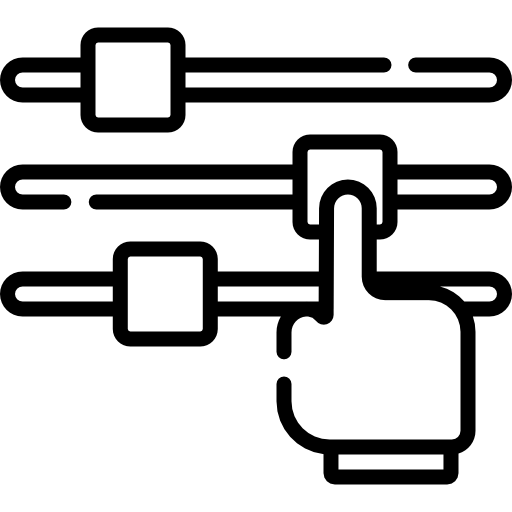
\includegraphics[width=.15\textwidth]{Fundamentação/Fatores Humanos/slider.png}}
        node(t_controlling)[below of = controlling,yshift = -0.75cm] {Controlling};
        
        \node (controls) [below of=controlling, yshift=-5cm,] {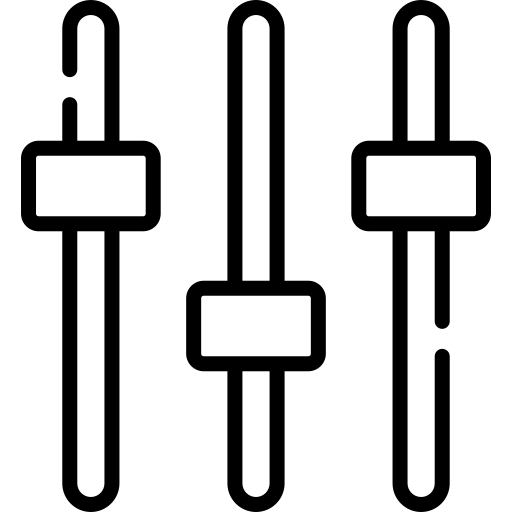
\includegraphics[width=.15\textwidth,angle=90,origin=c]{Fundamentação/Fatores Humanos/control.png}} 
        node(t_controls) [below of = controls, yshift = -0.75cm]{Controls};
        
        \node (machine) [left of=controls, xshift=-5cm, yshift=-2cm] {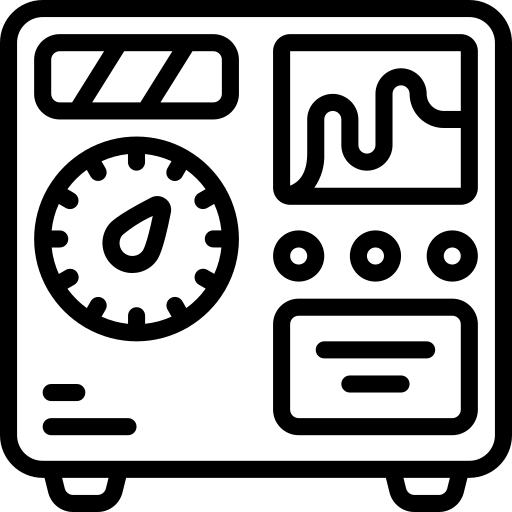
\includegraphics[width=.15\textwidth]{Fundamentação/Fatores Humanos/machine.png}} 
        node(t_machine) [below of = machine, yshift = -0.75cm]{Operation};
        
        \node (display) [left of=machine, xshift=-5cm, yshift=2cm] {
\includegraphics[width=.15\textwidth]{Fundamentação/Fatores Humanos/monitor.png}} 
        node(t_display) [below of = display, yshift = -0.75cm]{Display};
        
        \node (senses) [left of=information, xshift=-5cm, yshift=-2cm,] {\input{Fundamentação/Fatores Humanos/senses}} 
        node(t_senses) [below of = senses, yshift = -1.25cm]{Senses};
        
        \node (human) [below of=information, yshift=-4.75cm] {\Large{Human}};
        \node (human) [above of=machine, yshift=3.25cm] {\Large{Machine}};
        \node (human) [above of=information, yshift=1cm] {\Large{Work Environment}};
        
        \node (left_point) [left of=display, xshift=-2, yshift=2.75cm] {};
        \node (right_point) [right of=left_point, xshift=14cm] {};
        
        \node (input) [left of=machine, xshift=-5cm, yshift=-2cm] {\Large{Input}};
        \node (output) [right of=machine, xshift=5cm, yshift=-2cm] {\Large{Output}};
        
    
        \draw [arrow] (information.east) to (controlling.north west);
        \draw [arrow] (t_controlling.south) to (controls.north);
        \draw [arrow] (controls.west) to (machine.east);
        \draw [arrow] (machine.west) to (display.east);
        \draw [arrow] (display.north) to (t_senses.south);
        \draw [arrow] (senses.east) to (information.west);
        \draw [arrow] (input.east) -- (machine);
        \draw [arrow] (machine) -- (output.west);
        \draw [dashed,gray] (left_point) to (right_point);
        
        \draw (-8,-14) rectangle(8cm,1.5cm);
        
    \end{tikzpicture}
    }
    \caption{Human-Machine system representation \cite{sanders1998human}.}
    \label{fig:human_machine_representaion}
\end{figure}

\subsection{Mental Workload (MWL)}
\label{sec:mental_workload}

    Mental workload is one of the main concepts studied in Human Factors \cite{stanton2004handbook}.

In order to explain it, \citeonline{stanton2004handbook} propose an analogy with the concept of physical workload. When an athlete must lift a dumbbell (one of those gym weights bars), the strength demand from the athlete is proportional to the dumbbell’s mass being lifted. If the dumbbell is lighter than the athlete’s capability, then it is easy enough for him to lift it. If the athlete is strong enough to carry the dumbbell, he does not feel a physical demand bigger than his capabilities. In this case, the physical workload of this activity is properly fitted for this athlete. If the dumbbell is heavier than what the athlete can lift, then two things can happen: either the athlete adapts to lift that dumbbell using tools (adjust the strategy), or the athlete is not able to lift completely the dumbbell (performance degrades). It corresponds to the case of a person executing a task that is not fitted for his capabilities.

The mental workload is similar to the physical workload, but refers to the mental capacity necessary to perform a task. Each human being has a finite mental capacity. When the mental demand is higher than the operator’s capacity, the person needs to adapt in order to finish the task or the overall performance of the task is compromised. Otherwise, if the mental workload is too low, the operator may get bored and easily distracted and so could also fail or not process the task’s information.

It’s important to say that mental workload is unique within each individual and is influenced by his/her perception of the task but is also impacted by other factors outside the task itself and more related to the operator (like its skill, age, education, training) or the environment (like noise, heat and toxicity)  \cite{cain2007review, fallahi2016effects, cardoso2012evaluation}.

The mental workload is not a quantitative resource or something that one can directly measure, but a number of different methods have been proposed in the literature to infer it. Figure \ref{fig:mwl_overview} illustrates three different classes of methods to evaluate mental workload: methods based on task performance, methods based on physiological measures, and methods based on subjective questionnaires.
        
    \begin{figure}[!htb]
    \centering

    \tikzstyle{arrow} = [rounded corners, line width = 1mm, ->]
    
    \resizebox{0.85\width}{!}{
    \begin{tikzpicture}[node distance=1cm]
        
        \node (mwl) {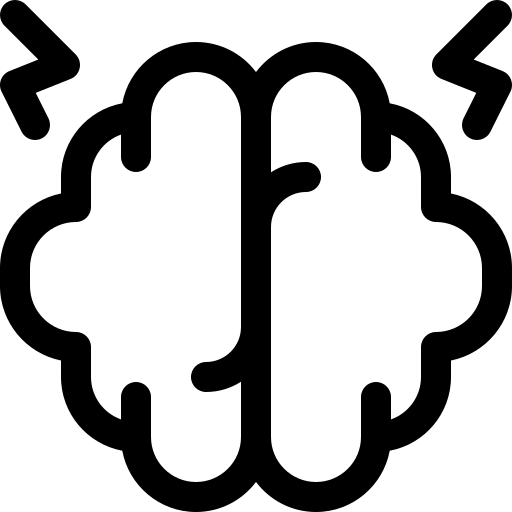
\includegraphics[width=.15\textwidth]{Fundamentação/Carga Mental/mwl.png}}
        node(t_mwl)[below of = mwl,yshift=-0.75cm] {Mental}
        node(t_mwl2)[below of = t_mwl,yshift=0.5cm] {workload};
        
        \node (demand) [above of=mwl, xshift=3cm, yshift=2.5cm] {\input{Fundamentação/Carga Mental/demand}}
        node(t_demand)[below of = demand,yshift=-0.75cm] {Task}
        node(t_demand2)[below of = t_demand,yshift=0.5cm] {Demand};
        
        \node (capacity) [above of=mwl, xshift=-3cm, yshift=2.5cm] {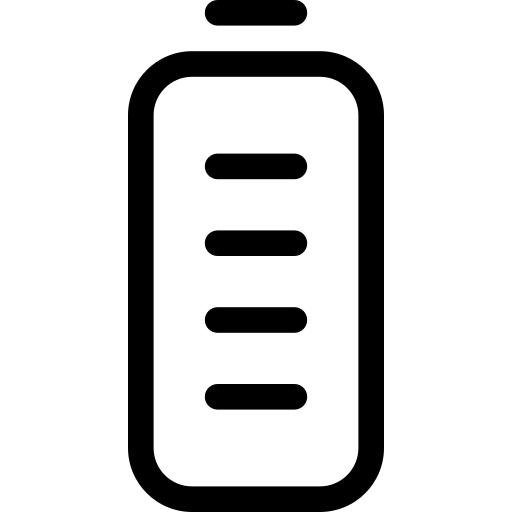
\includegraphics[width=.15\textwidth]{Fundamentação/Carga Mental/full-battery.png}}
        node(t_capacity)[below of = capacity,yshift=-0.75cm] {Mental}
        node(t_capacity2)[below of = t_capacity,yshift=0.5cm] {Capacity};
        
        \node (tasks) [left of=mwl, xshift=-4cm, yshift=-6cm] {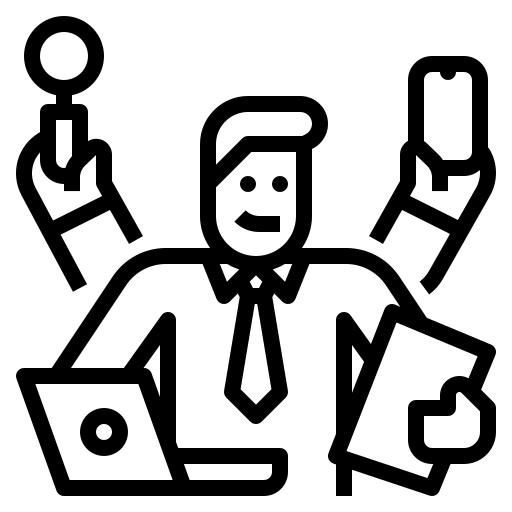
\includegraphics[width=.15\textwidth]{Fundamentação/Carga Mental/multitasking.png}}
        node(t_tasks)[below of = tasks,yshift = -0.75cm] {Primary and} 
        node(t_tasks2)[below of = t_tasks,yshift = 0.5cm] {secondary tasks};
        
        \node (physiological) [below of=mwl, yshift=-5cm,] {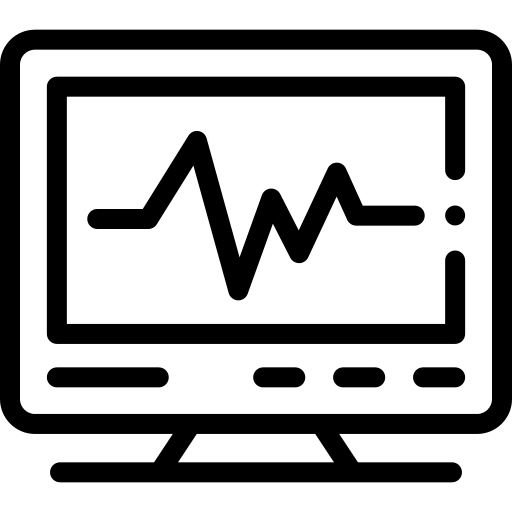
\includegraphics[width=.15\textwidth]{Fundamentação/Carga Mental/physiological.png}} 
        node(t_physiological) [below of = physiological, yshift = -0.75cm]{Physiological}
        node(t_physiological2) [below of = t_physiological, yshift = 0.5cm]{measurements};
        
        \node (subjective) [right of=mwl, xshift=4cm, yshift=-6cm] {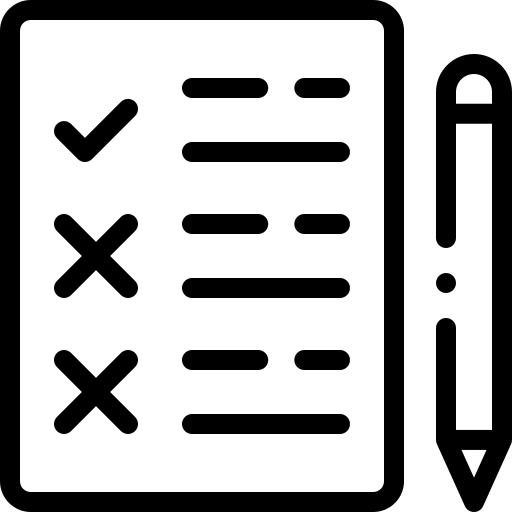
\includegraphics[width=.15\textwidth]{Fundamentação/Carga Mental/subjective.png}}
        node(t_subjective) [below of = subjective, yshift = -0.75cm]{Subjective} 
        node(t_subjective2) [below of = t_subjective, yshift = 0.5cm]{measurements};
    
    
        \draw [arrow] (t_mwl2.south) to ++(0,-0.75) to +(-5,0) to (tasks.north);
        \draw [arrow] (t_mwl2.south) to (physiological.north);
        \draw [arrow] (t_mwl2.south) to ++(0,-0.75) to +(5,0) to (subjective.north);
        \draw [arrow, sharp corners] (capacity.east) to +(1.6,0) to (mwl.north);
        \draw [arrow, sharp corners] (demand.west) -- +(-1.35,0) to (mwl.north);
    
        
    \end{tikzpicture}
    }
    \caption{A overview of mental workload and the methods to infer it.}
    \label{fig:mwl_overview}
\end{figure}    
    
    \subsubsection*{Methods based on task performance}
    %\label{subsec:task_performance}
    
        If the mental workload influences the task performance, then it would be possible to infer it using the performance’s variation of a task. Because there are cases where the user’s mental capacity is too high for only one task, a common approach is to add a secondary task. In this case, the user is asked to maintain a good performance level and still try to execute both tasks. Both tasks should use the same kind of skills \cite{stanton2004handbook, sanders1998human}.
        
        For example, an experiment to assess mental workload in a flight simulator may use two tasks, where the primary task is to fly the aircraft maintaining a given performance level, while the secondary task may be to mentally sum two random numbers that appear on the screen and, if the numbers’ sum is odd, then the pilot should press left on the keyboard else he/she should press right. If the pilot’s performance in the secondary task is too low, it means that the mental demand from the first task is too high for him/her to be able to pay attention to the secondary task \cite{mohanavelu2020cognitive}.
        
%    \item Physiological measures;
    \subsubsection*{Methods based on physiological measurements}
    %\label{subsec:physiological_measures}
    
        There are many physiological measurements that can be used to assess mental workload. Among the most common ones are the heart and brain activity \cite{chakladar2020eeg, orlandi2018measuring}, skin conductance, eye movement, pupillary contraction \cite{stanton2004handbook, rodriguez2015pupillometry}. These measurements are considered a good, unbiased assessment method \cite{fallahi2016effects}, but, still, it is recommended that they are evaluated alongside another method, as they may be influenced by unknown variables and external factors.

        This work uses the heart activity, obtained from an electrocardiogram (ECG) sensor, and the electrodermal activity, obtained from a galvanic skin response (GSR) sensor, as physiological measurements to assess mental workload.
                
        The electrocardiogram (ECG) is a recording of the heart’s electrical activity. From it, it is possible to determine the intervals between heartbeats and the corresponding frequency (heart rate, HR). Other common variable is the heart rate standard deviation (heart rate variability, HRV) \cite{cain2007review}. The heart activity is controlled by the sympathetic and parasympathetic nervous systems \cite{stanton2004handbook}. During a task, the heart activity changes with the mental demand of the task. The heart rate is expected to increase with the mental workload, while the heart rate variability is expected to decrease. These are consequences of two reactions in our system when in a mental demand situation \cite{stanton2004handbook}: a decrease in the parasympathetic nervous system activity and an increase in sympathetic nervous system activity. The ECG is a simple and non-invasive method used in many experiments to evaluate mental workload and other human factors’ \cite{mohanavelu2020cognitive, mansikka2016fighter, zhang2014detection}.
         %(DEFINIR MELHOR)
                
         The skin electrodermal activity is affected by the person’s sweating and the level of moisture in the environment. It can be used to reveal changes in our sympathetic system \cite{nourbakhsh2012using, shi2007galvanic}. It has been used in the literature as an assessment method for stress and arousal \cite{nourbakhsh2012using, stanton2004handbook, shi2007galvanic}, the usability of human-computer systems \cite{shi2007galvanic} and also mental workload \cite{zhang2014detection, borghini2014measuring}.
    
    \subsubsection*{Methods based on subjective questionnaires}
    %\label{subsec:subjective_measures}    

        The use of subjective questionnaires to assess mental workload has been extensively discussed in the literature \cite{sanders1998human, stanton2004handbook}. They are sensitive to perceived difficulty, automation, concurrent activities and demand for multiple resources. The questionnaires can be unidimensional, which are simpler but has only a general workload score 

        It is discussed if one should only use subjective measures to measure MWL \cite{sanders1998human, stanton2004handbook}. They are sensitive to perceived difficulty, automation, concurrent activities and demand for multiple resources. These test can be unidimensional, which are simpler but has only a general workload score \cite{stanton2004handbook},or multidimensional. Examples of multidimensional questionnaires are the Subjective Workload Assessment Technique (SWAT) and the NASA Task Load Index (NASA-TLX). SWAT decomposes the mental in three dimensions: time load; mental effort load; and psychological stress. NASA-TLX, a questionnaire created by \citeonline{hart1988development}, uses 6 different dimensions, as described in Table \ref{tab:nasa_dimensions}. These questionnaires were proposed evaluate only one task/activity. If the user has performed two tasks (a primary and secondary task), he/she should be oriented to answer about the primary task, not a combination of both of them \cite{sanders1998human}.
        
        \begin{table}[htb]
            \centering
            \caption{NASA-TLX dimensions and the description of each dimension. \cite{stanton2004handbook}.}
            \label{tab:nasa_dimensions}
                \begin{tabular}{|l|l|}

                    \hline
                    \textbf{Dimension}   & \textbf{Explanation}                                                                                                                                                   \\ \hline
                    Mental demand (MD)   & \begin{tabular}[c]{@{}l@{}}The mental and perceptive activity\\ demanded by the task (chose, decide,\\ think, calculate, search, etc.).\end{tabular}                       \\ \hline
                    Physical demand (PD) & \begin{tabular}[c]{@{}l@{}}The physical activity demanded by\\ the task (pull, lift, spin, drag, etc.).\end{tabular}                                                       \\ \hline
                    Temporal demand (TD) & \begin{tabular}[c]{@{}l@{}}The time pressure felt by the user.\\ A rating the leverages the time \\ available and the time necessary to\\ completed the task.\end{tabular} \\ \hline
                    Performance (PE)     & \begin{tabular}[c]{@{}l@{}}The user's satisfaction with its \\ performance or result the task.\end{tabular}                                                                \\ \hline
                    Effort (EF)          & \begin{tabular}[c]{@{}l@{}}A rating of the effort necessary \\ to achieve that performance felt by\\ the user.\end{tabular}                                                 \\ \hline
                    Frustration (FR)     & \begin{tabular}[c]{@{}l@{}}A rating of stress, annoy or irritation\\ felt by the user throughout the task.\end{tabular}                                                    \\ \hline
                \end{tabular}
        \end{table}
            
        Finally, it is important to highlight that, in order to have a comprehensive evaluation of the mental workload, it is recommended not to choose only one method, but to combine methods from the three classes (task performance, physiological measurements and subjective questionnaires). Mental workload is multidimensional and can reflect partially or differently in each of the methods \cite{sanders1998human}.

\subsection{Situation Awareness (SA)}
\label{sec:situation_awareness}

    Situation awareness can be defined as “the perception of the elements within a volume of time and space (Level 1), the comprehension of their meaning (Level 2), and the projection of their status in the near future (Level 3)” as illustrated in Figure \ref{fig:sa_overview}. One example is when an air traffic controller looks at a radar display (Level 1). He/she seeks to understand the aircraft's position and speed (Level 2) and then predict its position in the near future, 5, 10 or 15 minutes after (Level 3) \cite{sanders1998human}. Similarly, when a pilot reads the cockpit panel (Level 1) and understands their data (Level 2) then he/she can predict the next reading of that same instrument or some other status of the aircraft after a couple of minutes (Level 3).

The term “situation awareness” was first proposed for the Aeronautics domain and today is considered a key factor for designing complex and dynamic systems from other domains, such as automotive, medical and nuclear \cite{endsley1995measurement}. It is an essencial factor to make sure that the user will be capable to make important decisions correctly and achieve high-performance \cite{endsley1988design, endsley2018automation}.

\begin{figure}[!h]
    \centering
    \tikzstyle{arrow} = [rounded corners, line width = 1mm, ->]

    \resizebox{0.85\textwidth}{!}{
    \begin{tikzpicture}[node distance=3.3cm]
        \centering
        
        \node (info) [fill=white] {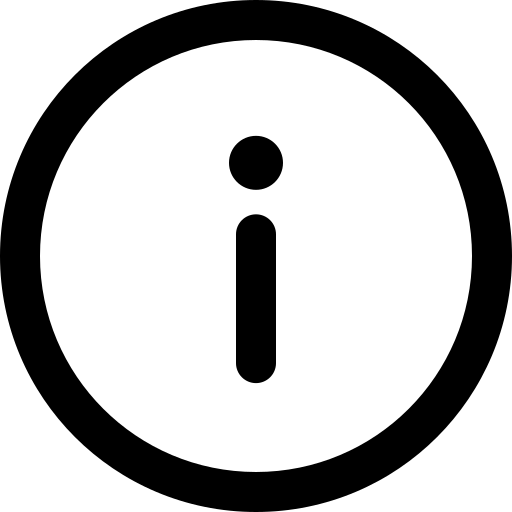
\includegraphics[width = 0.20\textwidth]{Fundamentação/Percepção situacional/information.png}}
        node(t_info)[below of = info,yshift=1.3cm] {\Large Information};
        
        \node (arrow) [right of=info, xshift=7.0cm, yshift = -0.5cm] {\input{Fundamentação/Percepção situacional/seta}};
        
        \node (perception) [right of=info, xshift=2.5cm, draw, line width=2mm] {\input{Fundamentação/Percepção situacional/perception}}
        node(t_perception)[below of = perception, yshift=0.9cm] {\Large 1st Level}
        node(t_perception2)[below of = t_perception, yshift=2.5cm] {\Large Perception};

        \node (comprehension) [right of=perception, xshift=0.25cm, draw, line width=2mm] {\input{Fundamentação/Percepção situacional/comprehension}}
        node(t_comprehension)[below of = comprehension, yshift=0.9cm] {\Large 2nd Level}
        node(t_comprehension2)[below of = t_comprehension, yshift=2.5cm] {\Large Comprehension};

        \node (projection) [right of=perception, xshift=3.75cm, draw, line width=2mm] {\input{Fundamentação/Percepção situacional/projection}}
        node(t_projection)[below of = projection, yshift=0.9cm] {\Large 3rd Level}
        node(t_projection2)[below of = t_projection, yshift=2.5cm] {\Large Projection};

        \node (decision) [right of=projection, xshift=5.0cm] {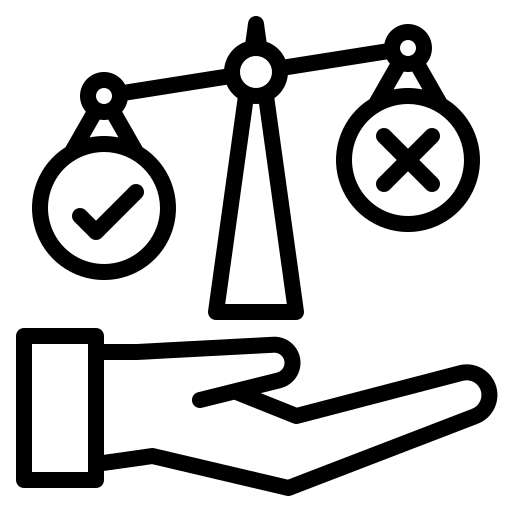
\includegraphics[width = 0.30\textwidth]{Fundamentação/Percepção situacional/decision.png}}
        node(t_decision)[below of = decision, yshift=0.5cm] {\Large Decision}
        node(t_decision2)[below of = t_decision, yshift=2.5cm] {\Large making};

    \end{tikzpicture}
    }
    \caption{An overview of situation awareness and the SAGAT.} %and the methods to infer it
    \label{fig:sa_overview}
\end{figure}

As it is for the mental workload, situation awareness is not a quantitative subject. The most common way to measure it is using subjective techniques, among which one of the most famous is the Situation Awareness Global Assessment Technique (SAGAT). It was proposed by \cite{endsley1988design} and is based on how the information is processed inside the user’s mind. The test application is made by freezing the operator activity, usually made in a simulation environment, and then asking the user some questions that were previously defined based on the user's activity. These questions should be as similar as possible to how the person thinks when reasoning about the situation to avoid extra effort in understanding it \cite{stanton2004handbook}.  Although freezing the activity may sound troublesome, empirical work has shown that it does not interfere with the user performance and the user memory can withstand a break for as long as 5 to 6 min \cite{endsley1988design}.


\section{Extended Reality (XR)}
\label{sec:extended_reality}

    Extended reality refers to the interaction of a Human-Machine system with a real and virtual interface together. It has four different forms:
\begin{itemize}
    \item Augmented Reality;
    \item Augmented Virtuality;
    \item Mixed Reality;
    \item Virtual Reality.
\end{itemize}

These forms differ from one another based on the leverage of reality and virtuality involved in the system. To help to visualise these differences, \citeonline{milgram1994taxonomy} created the concept of "virtuality continuum" and is presented on Figure \ref{fig:virtuality_continuum}. 

\begin{figure}[!h]
    \tikzstyle{arrow} = [ccmDBlue, rounded corners, line width = 2mm, ->]
    \tikzstyle{--blue} = [ccmDBlue, rounded corners, line width = 2mm]
    \tikzstyle{--black} = [rounded corners, line width = 1mm]
    
    %\tikzstyle{arrow_flow} = [ccmblue, rounded corners, line width = 2mm, ->]
    %\tikzstyle{arrow_return} = [ccmred, rounded corners, line width = 2mm, ->]
    
    \resizebox{0.80\width}{!}{
    \begin{tikzpicture}[node distance=1cm]
        \centering
    
        \node (left) {};
        
        \node (reality) [right of = left, xshift = 2cm]{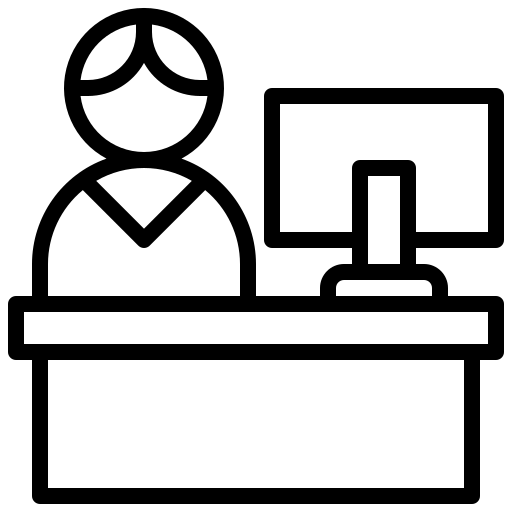
\includegraphics[width=.15\textwidth]{Fundamentação/Realidade Extendida/real.png}}
        node(t_reality)[below of = reality,yshift=-0.75cm] {Real}
        node(t_reality2)[below of = t_reality,yshift=0.5cm] {Environment};
        
        \node (midLeft) [right of = reality, xshift = 1cm] {};
        
        \node (ar) [right of=reality, xshift=3cm] {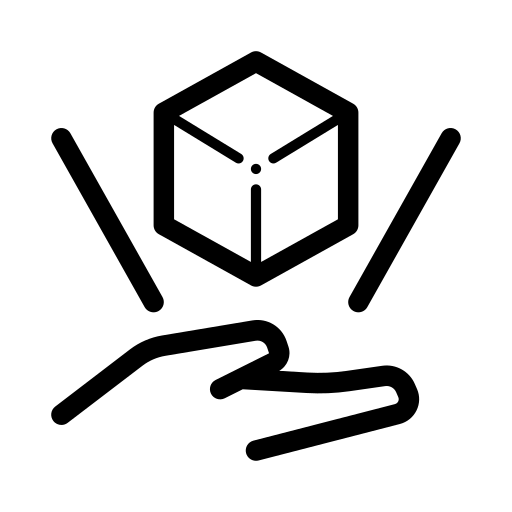
\includegraphics[width=.15\textwidth]{Fundamentação/Realidade Extendida/ar.png}}
        node(t_ar)[below of = ar,yshift=-0.75cm] {Augmented}
        node(t_ar2)[below of = t_ar,yshift=0.5cm] {Reality};
        
        \node (av) [right of=ar, xshift=3cm] {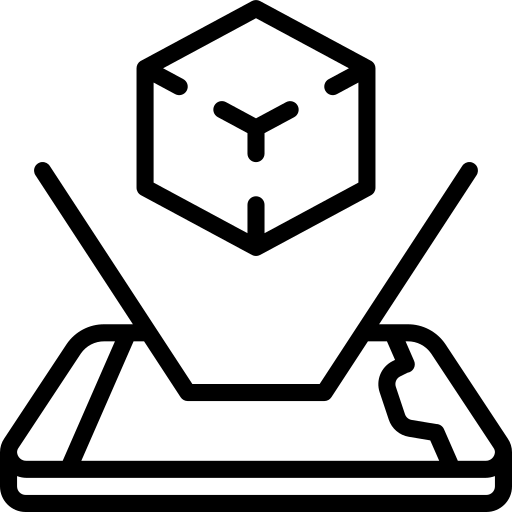
\includegraphics[width=.15\textwidth]{Fundamentação/Realidade Extendida/av.png}}
        node(t_av)[below of = av,yshift=-0.75cm] {Augmented}
        node(t_av2)[below of = t_av,yshift=0.5cm] {Virtuality};
        
        \node (vr) [right of=av, xshift=3cm] {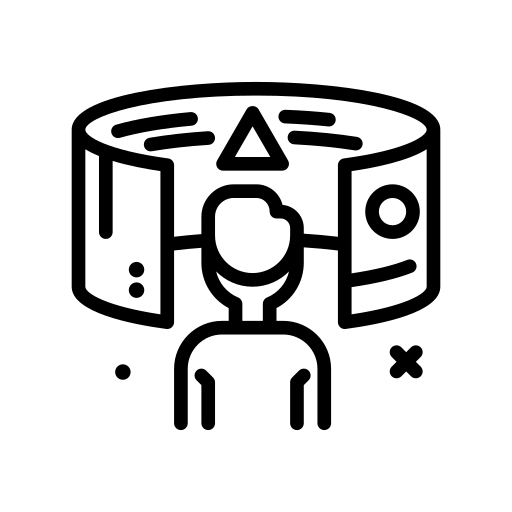
\includegraphics[width=.15\textwidth]{Fundamentação/Realidade Extendida/vr.png}}
        node(t_vr)[below of = vr,yshift = -0.75cm] {Virtual} 
        node(t_vr2)[below of = t_vr,yshift = 0.5cm] {Reality};
        
        \node (midRight) [left of = vr, xshift = -1cm] {};
        
        \node (right) [right of = vr, xshift = 2cm] {};
        
        \node (mr) [above of=ar, right of=ar, xshift=1cm, yshift=3cm] {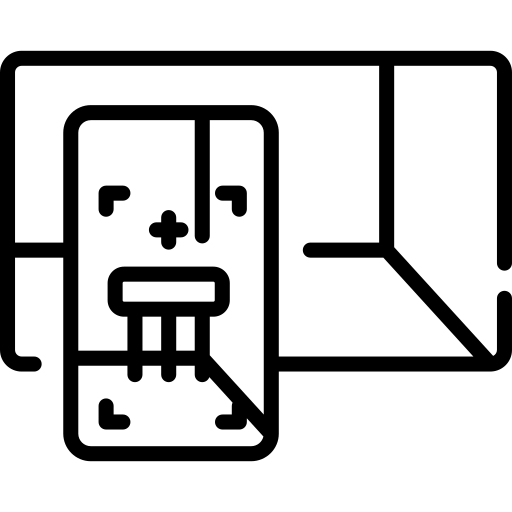
\includegraphics[width=.15\textwidth]{Fundamentação/Realidade Extendida/mr.png}} 
        node(t_mr) [below of = mr, yshift = -0.50cm]{Mixed}
        node(t_mr2) [below of = t_mr, yshift = 0.5cm]{Reality};
        
        \draw [arrow] (reality) to (left);
        \draw [--blue] (reality) to (ar);
        \draw [--blue] (ar) to (av);
        \draw [--blue] (av) to (vr);
        \draw [arrow] (vr) to (right);
        \draw [--black] (mr.west) -- +(-2.6,0) to (midLeft);
        \draw [--black] (mr.east) -- +(2.6,0) to (midRight);
         
        
        \node (left) [left of = reality, xshift = -2cm] {};
        \node (right) [right of = vr, xshift = 2cm] {};
    
        
    \end{tikzpicture}
    }
    \centering
    \caption{The Virtuality Continuum concept \cite{milgram1994taxonomy}}
    \label{fig:virtuality_continuum}
\end{figure}

The extreme left means full reality, where the stimuli does not come, or is not produced by any computer or any other digital system. Along the path to the right, the environment starts to have some digital elements until it reaches the far right, where all the elements in the environment have a digital origin \cite{nijholt2005virtuality, doolani2020review}. The first step from the Real Environment to Virtual Reality is the Augmented Reality.

\subsection{Augmented Reality (AR)}
\label{subsec:augmented_reality}

    In augmented reality, the user can see some digital elements, that could be text, images, video, etc, that are laid in a real environment without the user losing the sense of presence in the real world. Some uses for AR are to assist workers in the manufacturing, assembly tasks and training \cite{doolani2020review, farrell2018learning, ma2007virtuality}.

\subsection{Augmented Virtuality (AV)}
\label{subsec:augmented_virtuality}
    
    While AR brings digital elements inside a real environment, Augmented Virtuality creates an environment that could only exist with a digital origin, like a fantasy world from games or movies. This scenario is the background of some other activity that is being done in a real environment. An example could be using a virtual environment during a pilot or driver training or an engineer visualizing a real-time model of an aircraft in flight \cite{farshid2018go}. Other examples could be playing sports while using equipment to play it, like tennis, golf or baseball but the arena is completely digital. The user can use the real equipment with a tracker, but, besides that, the rest would be all digital.

\subsection{Mixed Reality (MR)}
\label{subsec:mixed_reality}

    Mixed Reality stays in between Real and Virtual Environments. But what is the difference between MR and AR or AV? In MR the user can manipulate digital elements as if they were inside the real world \cite{doolani2020review}. For example, a client from a furniture store could use MR to see what product fit inside his/her room. He/she can move the furniture inside the room and see if the colors, size and shape fit before buying or even going to the shop.
    
\subsection{Virtual Reality (VR)}
\label{subsec:virtual_reality}

    Resting in the far right of the virtuality continuum, the Virtual Reality has its user as the only element that hasn't a digital origin, making he/she immersed in a virtual environment, but, of course, inside the physical limits of a real environment \cite{ma2007virtuality}. If the feeling of presence of that environment is well done, the user can momentarily forget about the real environment and act and react accordingly to the virtual environment \cite{farrell2018learning}. 
    
    VR is a powerful tool that allows a user to be transported to a tridimensional environment that could be out of reach or that doesn't exist but is perfect to test or train some situation. Inside this virtual environment, the user can walk and look around and interact with the many elements as if they were real \cite{mujber2004virtual} and this technique becomes more effective and valuable when one can simulate a real situation and use it for training \cite{salah2019virtual}.
    
The Figure \ref{fig:ar_av_mr} shows the representations of each of these Extended Reality subsections.
    
\begin{figure}[!htb]
    \tikzstyle{arrow} = [ccmblue, rounded corners, line width = 2mm, ->]
    \tikzstyle{--blue} = [ccmblue, rounded corners, line width = 2mm]
    \tikzstyle{--black} = [rounded corners, line width = 1mm]
    
    \resizebox{0.85\width}{!}{
    \begin{tikzpicture}[node distance=1cm]
        \centering
    
        \node (ar) {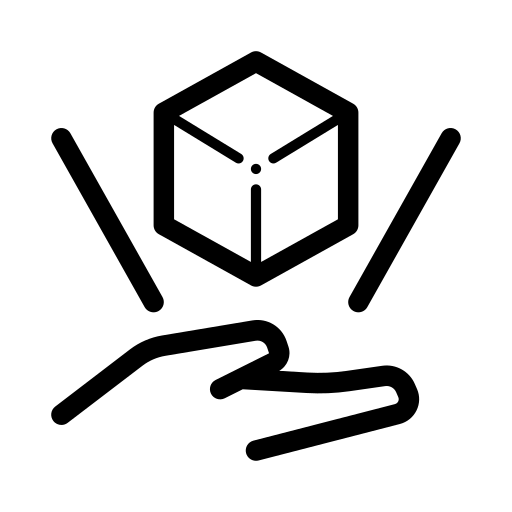
\includegraphics[width=0.3\textwidth]{Fundamentação/Realidade Extendida/ar.png}}
        node(t_ar)[below of = ar,yshift=-2.0cm] {Augmented}
        node(t_ar2)[below of = t_ar,yshift=0.5cm] {Reality};
        
        \node (av) [right of=ar, xshift=5cm, yshift = 0.1cm] {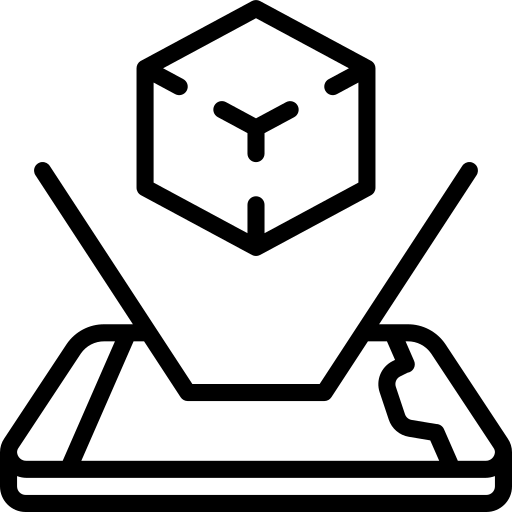
\includegraphics[width=.34\textwidth]{Fundamentação/Realidade Extendida/av.png}}
        node(t_av)[below of = av,xshift = 1.0cm, yshift=-2.0cm] {Augmented}
        node(t_av2)[below of = t_av,yshift=0.5cm] {Virtuality};
        
        \node (mr) [below of=ar, yshift=-5.5cm] {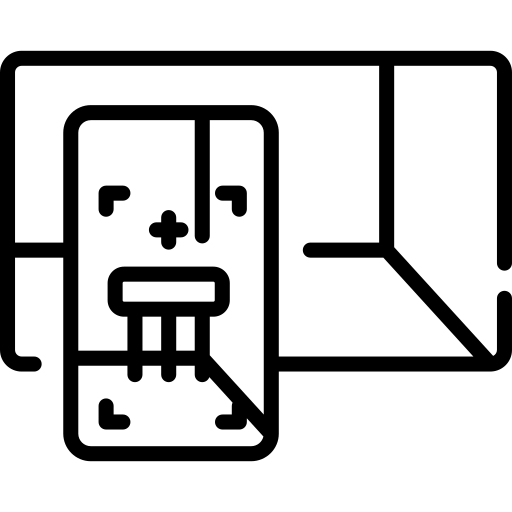
\includegraphics[width=.31\textwidth]{Fundamentação/Realidade Extendida/mr.png}}
        node(t_mr)[below of = mr,yshift=-2.0cm] {Mixed}
        node(t_mr2)[below of = t_mr,yshift=0.5cm] {Reality};
        
        \node (vr) [right of=mr, xshift=5.0cm, yshift = -0.5cm] {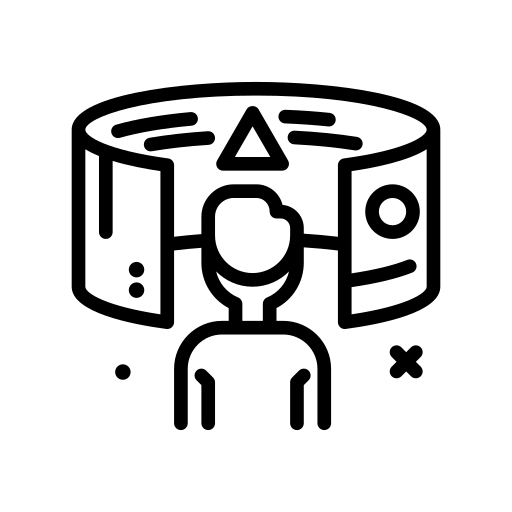
\includegraphics[width=.25\textwidth]{Fundamentação/Realidade Extendida/vr.png}}
        node(t_vr)[below of = vr,yshift = -1.5cm] {Virtual} 
        node(t_vr2)[below of = t_vr,yshift = 0.5cm] {Reality};
        
        \node (n) [right of = ar, above of = ar , xshift = 2cm, yshift = 3.0cm] {};
        \node (l) [right of = av, below of = av, xshift = 3cm, yshift = -3.1cm] {};
        \node (s) [left of = vr, below of = vr, xshift = -2cm, yshift = -3.0cm] {};
        \node (o) [left of = mr, above of = mr, xshift = -3cm, yshift = 1.6cm] {};
        
        
        %\draw [arrow] (reality) to (left);
        %\draw [--blue] (reality) to (ar);
        %\draw [--blue] (ar) to (av);
        %\draw [--blue] (av) to (vr);
        %\draw [arrow] (vr) to (right);
        \draw [--black] (n) to (s);
        \draw [--black] (l) to (o);
         
        
        %\node (left) [left of = reality, xshift = -2cm] {};
        %\node (right) [right of = vr, xshift = 2cm] {};
    
        
    \end{tikzpicture}
    }
    \centering
    \caption{A represantion of the differences between AR, AV, MR and VR. Made by the author}
    \label{fig:ar_av_mr}
\end{figure}    

\section{Co-Design}
\label{sec:co_design}

    Co-design, or collaborative design refers to a design process in which individuals of the design team have different backgrounds or bring different experiences, which can be important for the product under design. It is based on good communication and information sharing among the team \cite{chiu2002organizational}.

\citeonline{kleinsmann2006understanding} provides the following definition:.

\begin{quote}
    \textit{"Collaborative design is the process in which actors from different disciplines share their knowledge about both the design process and the design content. They do that to create a shared understanding of both aspects, to be able to integrate and explore their knowledge and to achieve the larger common objective: the new product to be designed."} \cite{kleinsmann2006understanding}.
\end{quote}

This definition emphasizes two key aspects of co-design: knowledge sharing and integration. According to \citeonline{kleinsmann2006understanding} knowledge is the data after the receiver’s understanding or translating process, in a state that is possible to record or register, in order that the person can remember and use it later. During the collaborative design, ideas, facts or concepts are exchanged between the actors. This exchange is a fundamental part of the co-design method since it is responsible for the growth of each individual’s knowledge. Once the knowledge is shared among the actors, it is possible for them to use it when performing their tasks, resulting in knowledge integration \cite{kleinsmann2006understanding}.

\section{Final remarks}
\label{sec:final_remarks2}

%Colocar um resumo do capitulo descrevendo também como os tres temas abordados são combinados no seu trabalho. Colocar uma seção de final remarks ao final de cada capitulo, com excecao do primeiro e do ultimo.

This chapter is dedicated to introducing the fundamental concepts, which are necessary for understanding the proposal of this Master's dissertation. It starts by describing the importance of Human Factors in improving human-machine interaction. Two important concepts of Human Factors are presented: mental workload and situation awareness. For each of them, the main assessment techniques are described.

Next, the concepts of extended and virtual reality are discussed, as well as other variations such as augmented reality and augmented virtuality. This work's idea is to explore the concept of using a virtual environment to quickly evaluate prototypes of assistive devices.

Finally, the approach of co-design is proposed as a way of integrating different stakeholders into the design process. 

The next chapter discusses recently published work that are related to the proposal of this work.


\chapter{Literature review}
\label{ch:revisao}
For the literature review of this work the following steps were taken to filter out the articles read.
\begin{itemize}
    \item Search through the Scopus and Web of Science platforms;
    \begin{itemize}
        \item Search the Scopus plaform:
        \begin{itemize}
            \item Filter articles using the keywords "Human Factors", "Virtual Reality";
            \item Filter articles from 2019 until 2022 and related to engineering or social science;
            \item Read the title and abstract and select the more relevant of them;
            \item Read the selected articles.
        \end{itemize}
        \item Search the Web of Science:
        \begin{itemize}
            \item Filter articles using the keywords "Human Factors", "Virtual Reality", "Covid-19" and "Blindness";
            \item Read the title and abstract and select the more relevant of them;
            \item Read the selected articles.
        \end{itemize}
    \end{itemize}
\end{itemize}

After following these steps, 344 abstracts were read and from these the following articles were selected as the most relevant for the research.

\section{Virtual Reality Without Vision}
\label{sec:vr_without_vision}
Motivated by the popularization of virtual reality technology, \citeonline{siu2020virtual} developed a white cane to be used by BVI users in a virtual environment. Their purpose was to make virtual reality applications available for BVI users. 

The traditional white cane transmits three sources of information to the user: detection of obstacles, surface topography and foot placement preview. In their work, these sources of information were transmitted through sounds or haptics \cite{siu2020virtual}, which would be defined based on the cane position in the virtual environment. For obstacle detection, the cane was built with a three-degree-of-freedom brake mechanism that would stop the movement when the cane hit an obstacle. A coil actuator was used to simulate surface properties. Lastly, a wave-based acoustic simulation was used to render geometry-aware sound effects in other to give the user a sense of the surroundings (echo localization).

In order to evaluate their proposal, the authors performed an experiment where the participants had to play a “scavenger hunt” using an HTC Vive system. During the experiment, each participant had two tasks: collect targets along the way (primary task) and avoid virtual obstacles and walls (secondary task). The targets appeared, one at a time, once the previous target was collected, and they emitted a sound that acted like an audio beacon for the participant. The obstacles did not emit any sound as a beacon, but the participant could detect it by the shape and the noise it emitted when in contact with the cane. The experiment was performed with 8 blind users (4 female, 4 male) from 25 to 70 years old. All of them did a training section where the virtual environment was presented. 

Among the relevant findings of \citeonline{siu2020virtual} is that not all the participants reacted the same to a particular stimulus. The vibration of the cane was considered confusing by some participants, while others were familiar with it. This difference affected the performance of the participants. The ones that had already used vibrating devices performed better. It shows that user's previous experiences can impact their performance in the virtual environment.

Another interesting observation was that, similar to what happens in the real world, it was easier for the participants to navigate in larger areas than in tight spaces. Moreover, the authors observed that the participants focused their attention on the primary task, without freely exploring the environment, which might have impacted the low time to achieve the goal and the low number of obstacle hits. 

Among the limitations pointed out by the authors is the lack of feedback possibilities for situations such as when the obstacle contacts a point along with the cane, not the tip of it, and the fact that the brake system did not stop the participant when he/she walked forwards toward a wall.

Comparing the work of \citeonline{siu2020virtual} to this work, \citeonline{siu2020virtual} were focused on providing mechanisms for a BVI user to navigate inside virtual environments. In this work, the purpose is to use the virtual environment to collect data about how the BVI user would navigate in a real environment. Another difference is in the functioning of the virtual cane, which in this work is limited to vibration, with no brake system, as the BVI user does not need to touch the environment with it. One common observation of both works is the sound importance for the BVI guidance and the need to use high-quality spatialized audio to increase the realism of the virtual environment.

\section{Effects of Emotion and Agency on Presence in Virtual Reality}
\label{sec:emotion_presence_vr}
The second work that discussed in this literature review is an evaluation of what affects the user’s feeling of presence in virtual reality, i.e., when the user feels drawn into the virtual environment and starts to occupy it instead of the real one \cite{cummings2016immersive}.


One of the many feelings that flourish during the use of a VR is the feeling of presence. This feeling, inside the virtuality context, is when someone feels drawn into a VE and starts to occupy the VE instead of the real one \cite{cummings2016immersive}.

\citeonline{jicol2021effects} aim to correlate the feeling of presence with one’s agency (which is the self-perception that the user is in control of a situation or some actions \cite{farrer2002experiencing} and emotion. For this purpose, the authors created two different virtual environment, one that would trigger happy emotions, and another that would trigger fear. For each of them, two variations were provided: one that the user could interact with (with agency) and another that it could not (without agency).

Following, they performed an experiment where 121 participants were randomly assigned to one of the four virtual environments. The purpose was to evaluate three hypotheses: 1) The intensity of the dominant emotion correlates positively with the presence; 2) Presence is significantly higher in environments where participants have agency; and 3) Agency moderates the effect of the emotion on the presence.

The results of the experiment confirmed the first hypothesis: no matter if the feeling was positive (happiness) or negative (fear), the users did feel a stronger presence when the positive or negative feelings were more intense. The second hypothesis was only partially confirmed. In the virtual environment that induced fear, agency did make a difference and induced a higher feeling of presence, whilst in the environment that induced happiness, agency did not affect the presence. The same could be said about the third hypothesis.

Although the study of \citeonline{jicol2021effects} was limited to sighted people, it highlights the importance of the feeling of presence for virtual reality. It provides important inputs to this work, such as the need of including mechanisms for the user to interact with the virtual environment in order to increase the feeling of presence. 


\section{Bradley and Dunlop research about BVI navigation}
\label{sec:bradley_dunlop}
Bradley and Dunlop published two works (\citeyear{bradley2002investigating,bradley2005experimental}) about how BVI navigates and how much it is similar or different to how a sighted person navigates. 

The first work of Bradley and Dunlop was published in \citeyear{bradley2002investigating} and discussed which type of information BVI uses to navigate in an environment and how it compares to sighted people. The data were collected during structured interviews where the participant had to explain how to arrive at two different locations as if they were talking to someone with the same vision condition \cite{bradley2002investigating}.

Based on the answers, the authors defined 11 categories of information: 1) directional (e.g. left/right, north/south); 2) structural (e.g. road, monument, church); 3) environmental (e.g. hill, river, tree); 4) textual-structural (e.g. name of shops, places, restaurants); 5) textual-area/street-based (e.g. name of street, neighbourhoods, squares); 6) numerical (e.g. first, second, 100m); 7) descriptive (e.g. steep, tall); 8) temporal/distance based (e.g. ”walk until you reach...” or ”before you get to”); 9) sensory (e.g. the sound of engines, the smell of bread from a bakery); 10) motion (e.g. cars passing by, doors opening); 11) social contact (e.g. asking people or using a guide dog for help) \cite{bradley2002investigating}.

As an output from the interviews, the authors provided the average number which each category was used by each group and is reproduced in Figure \ref{fig:bradley_2002}. From the results, the researchers observed that BVI participants used less text-based information than the sighted participants. However BVI participants used more words to describe a path than the sighted participants. Another essential result was that visually impaired people used, on average, 9 to 10 categories to describe a route, while sighted people used around 6 categories.

\begin{figure}[!htb]
    \centering
    \tikzstyle{barraVI} = [fill = cor1]
    \tikzstyle{barraS} = [fill = cor2]
    \tikzstyle{legenda} = [fill = white, line width = 0.25mm]
    \tikzstyle{--} = [line width = 0.25mm]
    
    \resizebox{0.8\linewidth}{!}{
    \begin{tikzpicture}[node distance=0cm]
        % Fundo do gráfico
    
        \renewcommand{\tamX}{13.875cm}
        \renewcommand{\tamY}{5.4cm}
        
        \node (origin) {};
        \node (endX) [xshift = \tamX] {};
        \node (endY) [yshift = \tamY] {};
        \node (endXY) [above of = endX, yshift = \tamY] {};
        
        %Título
        \node (titulo) [xshift = \tamX*0.5, yshift = \tamY + 1.25cm] {\textbf{Average nº of utterances used within each contextual category}}
        node [below of = titulo, yshift = -0.5cm] {\textbf{between sighted and visually impaired participants}};
        
        \draw[--] (origin.west) node[anchor = east]{\footnotesize 0} to (endX.center) node[anchor = north, xshift = -7.5cm, yshift = -2.0cm]{\textbf{Type of contextual categories}};
        \draw[--] (origin.south) to (endY.center) node[anchor = east, xshift = -1.0cm,rotate = 90]{\textbf{Average nº of utterance}};
        \draw[--] (endX.center) to (endXY.center);
        
        \foreach \r/\n in        {1/5,2/10,3/15,4/20,5/25,6/30,7/35,8/40,9/45,10/50,11/55,12/60,13/65,14/70,15/75,16/80,17/85,18/90}
        {
            \draw [--] (-0.15,0.30cm*\r) node[anchor = east]{\footnotesize \n} to (\tamX,0.30cm*\r);
        }
        
        \renewcommand{\largX}{0.25}
        \renewcommand{\altY}{0}
        \renewcommand{\distX}{0.5}
        %Direct
        \draw[barraVI] (\distX,0) node[yshift = -1.0cm, rotate = 45]{Direct} rectangle ++(\largX,5.3);
        \draw[barraS] (\distX+\largX,0) rectangle ++(\largX,1.6);
        \draw[--] (\distX+3.5*\largX,0) to ++(0,-0.2);
        
        \renewcommand{\distX}{1.75}
        %Struct
        \draw[barraVI] (\distX,0) node[yshift = -1.0cm, rotate = 45]{Struct} rectangle ++(\largX,3.6);
        \draw[barraS] (\distX+\largX,0) rectangle ++(\largX,0.5);
        \draw[--] (\distX+3.5*\largX,0) to ++(0,-0.2);
        
        \renewcommand{\distX}{3.0}
        %Struct
        \draw[barraVI] (\distX,0) node[yshift = -1.0cm, rotate = 45]{Environ} rectangle ++(\largX,0.5);
        \draw[barraS] (\distX+\largX,0) rectangle ++(\largX,0.2);
        \draw[--] (\distX+3.5*\largX,0) to ++(0,-0.2);
        
        \renewcommand{\distX}{4.25}
        %Struct
        \draw[barraVI] (\distX,0) node[yshift = -1.0cm, rotate = 45]{Text-struct} rectangle ++(\largX,0.2);
        \draw[barraS] (\distX+\largX,0) rectangle ++(\largX,0.4);
        \draw[--] (\distX+3.5*\largX,0) to ++(0,-0.2);
        
        \renewcommand{\distX}{5.5}
        %Struct
        \draw[barraVI] (\distX,0) node[yshift = -1.0cm, rotate = 45]{Text-area/st} rectangle ++(\largX,0.5);
        \draw[barraS] (\distX+\largX,0) rectangle ++(\largX,0.7);
        \draw[--] (\distX+3.5*\largX,0) to ++(0,-0.2);
        
        \renewcommand{\distX}{6.75}
        %Struct
        \draw[barraVI] (\distX,0) node[yshift = -1.0cm, rotate = 45]{Numer} rectangle ++(\largX,1.3);
        \draw[barraS] (\distX+\largX,0) rectangle ++(\largX,0.2);
        \draw[--] (\distX+3.5*\largX,0) to ++(0,-0.2);
        
        \renewcommand{\distX}{8.0}
        %Struct
        \draw[barraVI] (\distX,0) node[yshift = -1.0cm, rotate = 45]{Desc} rectangle ++(\largX, 4.2);
        \draw[barraS] (\distX+\largX,0) rectangle ++(\largX,0.45);
        \draw[--] (\distX+3.5*\largX,0) to ++(0,-0.2);
        
        \renewcommand{\distX}{9.25}
        %Struct
        \draw[barraVI] (\distX,0) node[yshift = -1.0cm, rotate = 45]{Sensory} rectangle ++(\largX,0.8);
        \draw[barraS] (\distX+\largX,0) rectangle ++(\largX,0.0);
        \draw[--] (\distX+3.5*\largX,0) to ++(0,-0.2);
        
        \renewcommand{\distX}{10.5}
        %Struct
        \draw[barraVI] (\distX,0) node[yshift = -1.0cm, rotate = 45]{Tem/Dist} rectangle ++(\largX,0.95);
        \draw[barraS] (\distX+\largX,0) rectangle ++(\largX,0.35);
        \draw[--] (\distX+3.5*\largX,0) to ++(0,-0.2);
        
        \renewcommand{\distX}{11.75}
        %Struct
        \draw[barraVI] (\distX,0) node[yshift = -1.0cm, rotate = 45]{Motion} rectangle ++(\largX,0.1);
        \draw[barraS] (\distX+\largX,0) rectangle ++(\largX,0.0);
        \draw[--] (\distX+3.5*\largX,0) to ++(0,-0.2);
        
        \renewcommand{\distX}{13.0}
        %Struct
        \draw[barraVI] (\distX,0) node[yshift = -1.0cm, rotate = 45]{Social} rectangle ++(\largX,0.2);
        \draw[barraS] (\distX+\largX,0) rectangle ++(\largX,0.0);
        \draw[--] (\distX+3.5*\largX,0) to ++(0,-0.2);
        
        %Legenda
        \draw[legenda] (\tamX-3.0cm,\tamY-1.5cm) rectangle (\tamX+1.5cm, \tamY+0.25cm);
        \draw[barraVI] (\tamX-2.5cm,\tamY-0.25cm) rectangle ++(0.25cm,0.25cm) node[anchor = west, xshift = 0.15cm, yshift = -0.15cm]{Visualy Impaired};
        \draw[barraS] (\tamX-2.5cm,\tamY-1.0cm) rectangle ++(0.25cm,0.25cm) node[anchor = west, xshift = 0.15cm, yshift = -0.15cm]{Sighted};
        
    \end{tikzpicture}
    }
    \centering
    \caption{Comparison between sighted participants with BVI participants (Adapted from \citeonline{bradley2002investigating}).}
    \label{fig:bradley_2002}
\end{figure}

Among the comments provided by BVI participants, a common one was about the limitations of available navigation options, such as white canes and guide dogs. They also emphasize that, when navigating, using different senses is essential for confirming one piece of information. 

To extend the findings of their previous work, Bradley and Dunlop designed an experiment to investigate if there is a difference between the perceived workload of BVI participants and sighted participants when they navigate using user-tailored information created with the results of the previous experiments \cite{bradley2005experimental}.

The experiment was performed with 16 participants, 8 sighted and 8 BVI, who were recruited to walk to four pre-determined landmarks in the centre of Glasgow. They followed the orientations recorded during the interviews from their previous work. For each participant, orientations for 2 of the 4 landmarks were made using sighted users' interviews, while the other 2 used data from BVI interviews. The results showed that BVI users reached landmarks significantly quicker when given the information made for that group, but still longer than sighted users. 

Another issue analysed during the experiment was the perceived workload. After each landmark, the participant was asked to complete the NASA-TLX questionnaire. The average score for each dimension of the NASA-TLX is reproduced in Figure \ref{fig:bradley_2005_participants}. As expected, it shows that BVI participants systematically have a higher workload than sighted participants. It also confirms that BVI did have a higher workload when guided by orientations provided by sighted people, as well as the sighted participants did with orientations from BVI. Another essential piece of information that stands out is the high frustration score given by the BVI users when they were guided by the orientations of sighted people.

\begin{figure}[htbp]
    \centering
    \begin{subfigure}{.49\textwidth}
        \centering
        \resizebox{\linewidth}{!}{
        \tikzstyle{barraVI} = [fill = cor1]
\tikzstyle{barraS} = [fill = cor2]
\tikzstyle{legenda} = [fill = white, line width = 0.25mm]
\tikzstyle{--} = [line width = 0.25mm]

%\resizebox{0.8\linewidth}{!}{
\begin{tikzpicture}[node distance=0cm]
    % Fundo do gráfico

    \renewcommand{\tamX}{12.0cm}
    \renewcommand{\tamY}{7.0cm}
    
    \node (origin) {};
    \node (endX) [xshift = \tamX] {};
    \node (endY) [yshift = \tamY] {};
    \node (endXY) [above of = endX, yshift = \tamY] {};
    
    %Título
    \node (titulo) [xshift = \tamX*0.5, yshift = \tamY + 1cm] {\textbf{\LARGE Comparing group scores for condition 1}};
    \draw[--] (origin.west) node[anchor = east]{\Large 0} to (endX.center) node[anchor = north, xshift = -\tamX*0.5, yshift = -1.0cm]{\textbf{\LARGE Workload dimensions}};
    \draw[--] (origin.south) to (endY.center) 
    node(eixoY)[anchor = east, xshift = -2.5cm, yshift = 0.5cm, rotate = 90]{\textbf{\LARGE Average weighted score}};
    \draw[--] (endX.center) to (endXY.center);
    
   \foreach \r/\n in {1/50,2/100,3/150,4/200,5/250,6/300, 7/350}
    {
        \draw [--] (-0.15,1cm*\r) node[anchor = east]{\Large \n} to (\tamX,1cm*\r);
    }
    
    \renewcommand{\largX}{0.5}
    \renewcommand{\altY}{0}
    \renewcommand{\distX}{0.5}
    
    %Mental Demand
    \draw[barraVI] (\distX,0) node[xshift = \largX*1cm, yshift = -0.5cm]{\textbf{\LARGE MD}} rectangle ++(\largX,6.1);
    \draw[barraS] (\distX+\largX,0) rectangle ++(\largX,2.8);
    \draw[--] (\distX+3*\largX,0) to ++(0,-0.2);
    
    \renewcommand{\distX}{2.5}
    %Physical Demand
    \draw[barraVI] (\distX,0) node[xshift = \largX*1cm, yshift = -0.5cm]{\textbf{\LARGE PD}} rectangle ++(\largX,0.3);
    \draw[barraS] (\distX+\largX,0) rectangle ++(\largX,0.5);
    \draw[--] (\distX+3*\largX,0) to ++(0,-0.2);
    
    \renewcommand{\distX}{4.5}
    %Temporal demand
    \draw[barraVI] (\distX,0) node[xshift = \largX*1cm, yshift = -0.5cm]{\textbf{\LARGE TD}} rectangle ++(\largX,0.9);
    \draw[barraS] (\distX+\largX,0) rectangle ++(\largX,0.7);
    \draw[--] (\distX+3*\largX,0) to ++(0,-0.2);
    
    \renewcommand{\distX}{6.5}
    %Performance
    \draw[barraVI] (\distX,0) node[xshift = \largX*1cm, yshift = -0.5cm]{\textbf{\LARGE OP}} rectangle ++(\largX,2.2);
    \draw[barraS] (\distX+\largX,0) rectangle ++(\largX,0.6);
    \draw[--] (\distX+3*\largX,0) to ++(0,-0.2);
    
    \renewcommand{\distX}{8.5}
    %Effort
    \draw[barraVI] (\distX,0) node[xshift = \largX*1cm, yshift = -0.5cm]{\textbf{\LARGE EF}} rectangle ++(\largX,4.1);
    \draw[barraS] (\distX+\largX,0) rectangle ++(\largX,2.3);
    \draw[--] (\distX+3*\largX,0) to ++(0,-0.2);
    
    \renewcommand{\distX}{10.5}
    %Frustation
    \draw[barraVI] (\distX,0) node[xshift = \largX*1cm, yshift = -0.5cm]{\textbf{\LARGE FR}} rectangle ++(\largX,3.7);
    \draw[barraS] (\distX+\largX,0) rectangle ++(\largX,0.2);
    \draw[--] (\distX+3*\largX,0) to ++(0,-0.2);
    
    
    %Legenda
    \draw[legenda] (\tamX-3.0cm,\tamY-1.5cm) rectangle ++(6.5cm,2cm);
    \draw[barraVI] (\tamX-2.75cm,\tamY-0.25cm) rectangle ++(0.25cm,0.25cm) 
    node[anchor = west, xshift = 0.15cm, yshift = -0.15cm]{\LARGE Visually impaired};
    \draw[barraS] (\tamX-2.75cm,\tamY-1.0cm) rectangle ++(0.25cm,0.25cm) 
    node[anchor = west, xshift = 0.15cm, yshift = -0.15cm]{\LARGE Sighted};
    
\end{tikzpicture}
%}
        }
        \caption{Condition 1.}
        \label{fig:bradley_2005_nasa_participants_1}
    \end{subfigure}
    \hfill
    \begin{subfigure}{.49\textwidth}
        \centering
        \resizebox{\linewidth}{!}{
        \tikzstyle{barraVI} = [fill = cor1]
\tikzstyle{barraS} = [fill = cor2]
\tikzstyle{legenda} = [fill = white, line width = 0.25mm]
\tikzstyle{--} = [line width = 0.25mm]

%\resizebox{0.8\linewidth}{!}{
\begin{tikzpicture}[node distance=0cm]
    % Fundo do gráfico

    \renewcommand{\tamX}{12.0cm}
    \renewcommand{\tamY}{6.0cm}
    
    \node (origin) {};
    \node (endX) [xshift = \tamX] {};
    \node (endY) [yshift = \tamY] {};
    \node (endXY) [above of = endX, yshift = \tamY] {};
    
    %Título
    \node (titulo) [xshift = \tamX*0.5, yshift = \tamY + 1cm] {\textbf{\LARGE Orientation from BVI people}};
    \draw[--] (origin.west) node[anchor = east]{\Large 0} to (endX.center) node[anchor = north, xshift = -\tamX*0.5, yshift = -5.0cm]{\textbf{\LARGE Workload dimensions}};
    \draw[--] (origin.south) to (endY.center) 
    node(eixoY)[anchor = east, xshift = -2.5cm, yshift = 0.5cm, rotate = 90]{\textbf{\LARGE Average weighted score}};
    \draw[--] (endX.center) to (endXY.center);
    
    \foreach \r/\n in {1/50,2/100,3/150,4/200,5/250,6/300}
    {
        \draw [--] (-0.15,1cm*\r) node[anchor = east]{\Large \n} to (\tamX,1cm*\r);
    }
    
    \renewcommand{\largX}{0.5}
    \renewcommand{\altY}{0}
    \renewcommand{\distX}{0.5}
    
    %Mental Demand
    %\draw[barraVI] (\distX,0) node[xshift = \largX*1cm, yshift = -0.5cm]{\textbf{\LARGE MD}} rectangle ++(\largX,5.6);
    \draw[barraVI] (\distX,0) node[xshift = \largX*-1.65cm, yshift = -2.25cm]{\rotatebox{50}{\textbf{\LARGE Mental Demand}}} rectangle ++(\largX,5.6);
    \draw[barraS] (\distX+\largX,0) rectangle ++(\largX,3.1);
    \draw[--] (\distX+3*\largX,0) to ++(0,-0.2);
    
    \renewcommand{\distX}{2.5}
    %Physical Demand
    %\draw[barraVI] (\distX,0) node[xshift = \largX*1cm, yshift = -0.5cm]{\textbf{\LARGE PD}} rectangle ++(\largX,0.7);
    \draw[barraVI] (\distX,0) node[xshift = \largX*-1.75cm, yshift = -2.25cm]{\rotatebox{50}{\textbf{\LARGE Physical Demand}}} rectangle ++(\largX,0.7);
    \draw[barraS] (\distX+\largX,0) rectangle ++(\largX,0.5);
    \draw[--] (\distX+3*\largX,0) to ++(0,-0.2);
    
    \renewcommand{\distX}{4.5}
    %Temporal demand
    %\draw[barraVI] (\distX,0) node[xshift = \largX*1cm, yshift = -0.5cm]{\textbf{\LARGE TD}} rectangle ++(\largX,0.9);
    \draw[barraVI] (\distX,0) node[xshift = \largX*-2cm, yshift = -2.5cm]{\rotatebox{50}{\textbf{\LARGE Temporal Demand}}} rectangle ++(\largX,0.9);
    \draw[barraS] (\distX+\largX,0) rectangle ++(\largX,0.7);
    \draw[--] (\distX+3*\largX,0) to ++(0,-0.2);
    
    \renewcommand{\distX}{6.5}
    %Performance
    %\draw[barraVI] (\distX,0) node[xshift = \largX*1cm, yshift = -0.5cm]{\textbf{\LARGE OP}} rectangle ++(\largX,2.1);
    \draw[barraVI] (\distX,0) node[xshift = \largX*-1.25cm, yshift = -1.65cm]{\rotatebox{50}{\textbf{\LARGE Performance}}} rectangle ++(\largX,2.1);
    \draw[barraS] (\distX+\largX,0) rectangle ++(\largX,0.5);
    \draw[--] (\distX+3*\largX,0) to ++(0,-0.2);
    
    \renewcommand{\distX}{8.5}
    %Effort
    %\draw[barraVI] (\distX,0) node[xshift = \largX*1cm, yshift = -0.5cm]{\textbf{\LARGE EF}} rectangle ++(\largX,3.8);
    \draw[barraVI] (\distX,0) node[xshift = \largX*-0.0cm, yshift = -0.850cm]{\rotatebox{50}{\textbf{\LARGE Effort}}} rectangle ++(\largX,3.8);
    \draw[barraS] (\distX+\largX,0) rectangle ++(\largX,2.5);
    \draw[--] (\distX+3*\largX,0) to ++(0,-0.2);
    
    \renewcommand{\distX}{10.5}
    %Frustation
    %\draw[barraVI] (\distX,0) node[xshift = \largX*1cm, yshift = -0.5cm]{\textbf{\LARGE FR}} rectangle ++(\largX,1.5);
    \draw[barraVI] (\distX,0) node[xshift = \largX*-1.0cm, yshift = -1.35cm]{\rotatebox{50}{\textbf{\LARGE Frustation}}} rectangle ++(\largX,1.5);
    \draw[barraS] (\distX+\largX,0) rectangle ++(\largX,1.1);
    \draw[--] (\distX+3*\largX,0) to ++(0,-0.2);
    
    
    %Legenda
    \draw[legenda] (\tamX-3.0cm,\tamY-1.5cm) rectangle ++(6.5cm,2cm);
    \draw[barraVI] (\tamX-2.75cm,\tamY-0.25cm) rectangle ++(0.25cm,0.25cm) 
    node[anchor = west, xshift = 0.15cm, yshift = -0.15cm]{\LARGE BVI};
    \draw[barraS] (\tamX-2.75cm,\tamY-1.0cm) rectangle ++(0.25cm,0.25cm) 
    node[anchor = west, xshift = 0.15cm, yshift = -0.15cm]{\LARGE Sighted};
    
\end{tikzpicture}
%}
        }
        \caption{Condition 2.}
        \label{fig:bradley_2005_nasa_participants_2}
    \end{subfigure}
\caption{Comparison of the NASA-TLX between the participants (Adapted from \citeonline{bradley2005experimental}).}
\label{fig:bradley_2005_participants}
\end{figure}

The work of \citeonline{bradley2002investigating} brings some relevant information for developing this work. Firstly, it shows the differences between the way sighted and BVI people navigate, highlighting the importance of including BVI in the design process of assistive technologies. It confirms the limitations of the current solutions. It brings essential insights on what type of information to include in developing audio systems, which is one of the assistive devices evaluated in this work. Finally, it shows the importance of using different workload assessment techniques when evaluating assistive technologies.

\section{Evaluation of spatial display for navigation without sight}
\label{sec:evaluation_spatial_display}
\citeonline{marston2006evaluation} presents a comparison of assistive devices for BVI. Two guidance displays were evaluated, one based on haptics and another based on sound. They were tested in two different scenarios: a busy street block, with a variety of street furniture, parked bicycles and people, and a park, with paths made of concrete, crushed gravel and paver blocks. 

The experiment was performed with 8 BVI participants. As output, the authors collected the time to reach a set of waypoints, the errors made by the participants, the travelled distance and the percentage of the total time that the users accessed the guidance device. All participants were able to complete the task with both devices. However, the configuration (audio x haptic, street x park) that resulted in the best performance varied among the participants. One relevant consideration is that the haptic device caused strain on the participants’ arm and was considered less acceptable, when compared to the sound device, which required no use of the arms.

Similar to the study of \citeonline{marston2006evaluation}, this work also compares different devices, based on haptics and sound. But, complementary to \citeonline{marston2006evaluation}, this work also evaluates the combined use of devices, as well as how they compare to the guidance system current in use by the BVI participant. 

\section{Use of VR in the aircraft cabin design process}
\label{sec:vr_cabin}
% \lipsum[2-4]

The use of virtual reality for design purposes is not new. It has been studied and evaluated in several areas, including Aeronautics. \citeonline{moerland2021application} investigated using virtual reality during the aircraft cabin’s design process with the purpose of facilitating the communication between the design team and the client. 

The cabin design process (Figure \ref{fig:simplified_cabin_process}) is often said to be complex because it involves several stakeholders, each with his/her own set of preferences and requirements. According to the authors, the time needed to satisfy the multiple demands tends to be long, and the process usually requires building multiple mock-ups and attending many meetings with the stakeholders. 

\begin{figure}[!htbp]
    \centering    
    \tikzstyle{hexag} = [regular polygon, regular polygon sides=6, minimum size = 3cm, inner sep = 0cm, xshift = 1.5cm]
    \tikzstyle{hexagText} = [text = white, xshift = 1.5cm]
    \tikzstyle{legenda} = [fill = white, line width = 0.25mm]
    \tikzstyle{--} = [line width = 0.25mm]
    
    \tikzstyle{arrow} = [rounded corners, line width = 1mm, -to]
    \tikzstyle{arrow_blue} = [cor5, arrow]
    
    \resizebox{\linewidth}{!}{
    \begin{tikzpicture}[node distance=1.75cm]
        \centering    

        \node [hexag, draw = cor1, fill = cor1] (emphatize) {};
        \node [hexagText] (emphatizeText) {};
        
        \node [hexag, draw = cor2, fill = cor2, right of = emphatize] (define) {};
        \node [hexagText, right of = emphatize] (defineText) {DEFINE};
        
        \node(inicioFlecha1) [xshift = 3.75cm, yshift = 2.25cm] {};
        \node(fimFlecha1) [right of = emphatize, xshift = 1cm, yshift = 1.2cm] {};
        \node(inicioFlecha2) [xshift = 2.75cm, yshift = 1.5cm] {};
        \node(fimFlecha2) [right of = emphatize, xshift = 0.5cm, yshift = 0.8cm] {};
        \node(inicioFlecha3) [xshift = 1.7cm, yshift = 0.8cm] {};
        \node(fimFlecha3) [right of = emphatize, xshift = 0.25cm, yshift = 0.4cm] {};
        \node(inicioFlecha4) [xshift = 2cm, yshift = -0.5cm] {};
        \node(fimFlecha4) [right of = emphatize, xshift = 0.15cm, yshift = 0cm] {};
        \node(inicioFlecha5) [xshift = 2.77cm, yshift = -1.6cm] {};
        \node(fimFlecha5) [right of = emphatize, xshift = 0.25cm, yshift = -0.5cm] {};
        \node(inicioFlecha6) [xshift = 3.4cm, yshift = -2.2cm] {};
        \node(fimFlecha6) [right of = emphatize, xshift = 0.8cm, yshift = -1.2cm] {};
        
        \draw[arrow] (inicioFlecha1) .. controls ++(0.3,-0.5) .. (fimFlecha1);
        \draw[arrow] (inicioFlecha2) .. controls ++(0.5,-0.15) .. (fimFlecha2);
        \draw[arrow] (inicioFlecha3) .. controls ++(0.75,0) .. (fimFlecha3);
        \draw[arrow] (inicioFlecha4) .. controls ++(0.5,0.25) .. (fimFlecha4);
        \draw[arrow] (inicioFlecha5) .. controls ++(0.25,0.5) .. (fimFlecha5);
        \draw[arrow] (inicioFlecha6) .. controls ++(0.25,0.5) .. (fimFlecha6);
        
        \node [hexag, draw = cor3, fill = cor3, right of = define] (ideate) {};
        \node [hexagText, right of = define] (ideateText) {IDEATE};
        
        \node(inicioDFlecha1) [above of = define, xshift = 0.25cm, yshift = -0.1cm] {};
        \node(fimDFlecha1) [above of = ideate, xshift = -0.25cm, yshift = -0.1cm] {};
        \node(inicioIFlecha1) [below of = ideate, xshift = -0.25cm, yshift = 0.1cm] {};
        \node(fimIFlecha1) [below of = define, xshift = 0.25cm, yshift = 0.1cm] {};
        
        \draw[arrow, draw = cor3] (inicioDFlecha1.south) .. controls ++(0.25,0.5) and ++(-0.75,0.5).. (fimDFlecha1.south);
        \draw[arrow, draw = cor3] (inicioIFlecha1.north) .. controls ++(-0.25,-0.5) and ++(0.75,-0.5).. (fimIFlecha1.north);
        
        \node [hexag, draw = cor4, fill = cor4, right of = ideate] (prototype) {};
        \node [hexagText, right of = ideate] (prototypeText) {PROTOTYPE};
        
        \node(inicioIFlecha2) [above of = ideate, xshift = 0.25cm, yshift = -0.2cm] {};
        \node(fimIFlecha2) [above of = prototype, xshift = -0.25cm, yshift = -0.2cm] {};
        \node(inicioPFlecha1) [below of = prototype, xshift = -0.25cm, yshift = 0.2cm] {};
        \node(fimPFlecha1) [below of = ideate, xshift = 0.25cm, yshift = 0.2cm] {};
        \node(inicioPFlecha2) [above of = prototype, xshift = 0.25cm, yshift = -0.2cm] {};
        \node(fimPFlecha2) [above of = define, xshift = -0.25cm, yshift = -0.2cm] {};
        
        \draw[arrow, draw = cor4] (inicioIFlecha2.center) .. controls ++(0.25,0.5) and ++(-0.75,0.5).. (fimIFlecha2.east);
        \draw[arrow, draw = cor4] (inicioPFlecha1.east) .. controls ++(-0.25,-0.5) and ++(0.75,-0.5).. (fimPFlecha1.center);
        \draw[arrow, draw = cor1] (inicioPFlecha2.west) .. controls ++(-1,1.75) and ++(1.2,1.5).. (fimPFlecha2);
        
        
        \node [hexag, draw = cor5, fill = cor5, right of = prototype] (assess) {};
        
        \node(inicioPFlecha3) [above of = prototype, xshift = 0.25cm, yshift = -0.2cm] {};
        \node(fimPFlecha3) [above of = assess, xshift = -0.25cm, yshift = -0.2cm] {};
        \node(inicioAFlecha1) [below of = assess, xshift = -0.25cm, yshift = 0.2cm] {};
        \node(fimAFlecha1) [below of = prototype, xshift = 0.25cm, yshift = 0.2cm] {};
        \node(inicioAFlecha2) [below of = assess, xshift = 0cm, yshift = 0.2cm] {};
        \node(fimAFlecha2) [below of = ideate, xshift = -0.25cm, yshift = 0.1cm] {};
        \node(inicioAFlecha3) [below of = assess, xshift = 0.25cm, yshift = 0.2cm] {};
        \node(fimAFlecha3) [below of = define, xshift = -0.25cm, yshift = 0.1cm] {};
        
        \draw[arrow, draw = cor5] (inicioPFlecha3.center) .. controls ++(0.5,1) and ++(-0.75,1).. (fimPFlecha3.center);
        \draw[arrow, draw = cor5] (inicioAFlecha1.center) .. controls ++(-0.25,-0.5) and ++(0.75,-1).. (fimAFlecha1.west);
        \draw[arrow, draw = cor2] (inicioAFlecha2.center) .. controls ++(-0.25,-1.25) and ++(0.75,-1).. (fimAFlecha2.south east);
        \draw[arrow, draw = cor1] (inicioAFlecha3.center) .. controls ++(-0.25,-1.75) and ++(1.2,-1.5).. (fimAFlecha3.north);
        
        \node [hexagText, right of = prototype] (assessText) {ASSESS};
        

        
        
    \end{tikzpicture}
    }
    \caption{Simplified cabin design process (Adapted from \citeonline{moerland2021application}).}
    \label{fig:simplified_cabin_process}
\end{figure}

\citeonline{moerland2021application} proposed to anticipate the involvement of the final users based on co-design. In their proposal, the users can influence the product's development from the beginning, as shown in Figure \ref{fig:user_involvement}. However, for the involvement to happen, a communication channel needed to be established, and it was done using virtual reality.

\begin{figure}[!htbp]
    \centering    
    \tikzstyle{hexag} = [regular polygon, regular polygon sides=6, minimum size = 3cm, inner sep = 0cm, xshift = 1.5cm]
    \tikzstyle{hexagText} = [text = white, xshift = 1.5cm]
    \tikzstyle{legenda} = [fill = white, line width = 0.25mm]
    \tikzstyle{--} = [line width = 0.25mm]
    
    \resizebox{\linewidth}{!}{
    \begin{tikzpicture}[node distance=1.75cm]
        \centering    

        \node [hexag, draw = cor1, fill = cor1] {};
        \node [hexagText] (emphatize) {EMPHATIZE};
        %\node [regular polygon, regular polygon sides=6, text = white, draw = cor1, minimum size = 5cm, fill = cor1] (emphatize) {EMPHATIZE};
        \node [hexag, draw = cor2, fill = cor2, right of = emphatize] (define) {};
        \node [hexagText, right of = emphatize] (defineText) {DEFINE};
        %\node [regular polygon, regular polygon sides=6, text = white, draw = cor2, minimum size = 5cm, fill = cor2, right of = emphatize] (define) {DEFINE};
        \node [hexag, draw = cor3, fill = cor3, right of = define] (ideate) {};
        \node [hexagText, right of = define] (ideateText) {IDEATE};
        %\node [regular polygon, regular polygon sides=6, text = white, draw = cor3, minimum size = 5cm, fill = cor3, right of = define] (ideate) {IDEATE};
        \node [hexag, draw = cor4, fill = cor4, right of = ideate] (prototype) {};
        \node [hexagText, right of = ideate] (prototypeText) {PROTOTYPE};
        %\node [regular polygon, regular polygon sides=6, text = white, draw = cor4, minimum size = 5cm, fill = cor4, right of = ideate] (prototype) {PROTOTYPE};
        \node [hexag, draw = cor5, fill = cor5, right of = prototype] (assess) {};
        \node [hexagText, right of = prototype] (assessText) {ASSESS};
        %\node [regular polygon, regular polygon sides=6, text = white, draw = cor5, minimum size = 5cm, fill = cor5, right of = prototype] (assess) {ASSESS};

        \node(insertNorth1) [right of = emphatize, xshift = -0.125cm, yshift = 0.25cm] {};
        \node(insertNorthWest1) [above of = insertNorth1, left of = insertNorth1, xshift = 0.75cm] {};
        \node(insertNorthEast1) [above of = insertNorth1, right of = insertNorth1, xshift = -0.75cm] {};
        \draw[--] (insertNorthWest1.center) to (insertNorth1.center) to (insertNorthEast1.center);
        
        \node(insertSouth1) [right of = emphatize, xshift = -0.125cm, yshift = -0.25cm] {};
        \node(insertSouthWest1) [below of = insertSouth1, left of = insertSouth1, xshift = 0.75cm] {};
        \node(insertSouthEast1) [below of = insertSouth1, right of = insertSouth1, xshift = -0.75cm] {};
        \draw[--] (insertSouthWest1.center) to (insertSouth1.center) to (insertSouthEast1.center);
        
        \node(insertNorth2) [right of = define, xshift = -0.125cm, yshift = 0.25cm] {};
        \node(insertNorthWest2) [above of = insertNorth2, left of = insertNorth2, xshift = 0.75cm] {};
        \node(insertNorthEast2) [above of = insertNorth2, right of = insertNorth2, xshift = -0.75cm] {};
        \draw[--] (insertNorthWest2.center) to (insertNorth2.center) to (insertNorthEast2.center);
        
        \node(insertSouth2) [right of = define, xshift = -0.125cm, yshift = -0.25cm] {};
        \node(insertSouthWest2) [below of = insertSouth2, left of = insertSouth2, xshift = 0.75cm] {};
        \node(insertSouthEast2) [below of = insertSouth2, right of = insertSouth2, xshift = -0.75cm] {};
        \draw[--] (insertSouthWest2.center) to (insertSouth2.center) to (insertSouthEast2.center);


    \end{tikzpicture}
    }
    \caption{Best moments for user involvement \cite{moerland2021application}.}
    \label{fig:user_involvement}
\end{figure}

The authors described the application of the proposed approach to a use case. Three different designers initiated a cabin design. In the traditional method, the results were illustrated in a sketch, which could only present a glance of what the cabin would be, and in a 3D model, which had more details. However, any modification required a new rendering session and this could take hours, or even days. The same solution was also illustrated in a virtual reality environment. The sketch was inside the aircraft cabin, where the client or the stakeholder could draw and give their opinions from the beginning of the design process. The 3D models could be imported to increase the sketch's level of detail.

The use case showed some benefits and disadvantages of using virtual reality. The virtual reality helped to bring the client closer to the design team, allowing them to draw quick sketches in brainstorming gatherings. It was associated with a steep learning curve for the designers. Among the disadvantages, it was considered a high-cost tool, and its use for a long time was associated with nausea. 

The work of \citeonline{moerland2021application} is an example of how virtual reality can be used to bring the user into the design process. Similarly, in this work, virtual reality is explored to create a test environment where BVI users can try out the device under development, contributing to improving its usability. Differently from the work of \citeonline{moerland2021application}, in this work, users are not expected to feel sick, as it is usually associated with discrepancies between the motion of the image in the virtual environment and the motion perceived by the vestibular system of the user.

\chapter{Proposal description}
\label{ch:metodologia}
% CAPÍTULO 3: DESCRIÇÃO DA SUA PROPOSTA OU CONTRIBUIÇÃO
%   ESSE É O CAPÍTULO MAIS IMPORTANTE DE SEU TRABALHO


%1. Elabore um parágrafo que introduz o capítulo: Este capítulo apresenta(descreva o objetivo do  capítulo...). É constituído de N seções a saber...
%2. Caso você tenha dúvida do nível de detalhamento da descrição, coloque-se no lugar do leitor!
%3. Elabore um parágrafo que conclui o capítulo e introduz o capítulo seguinte.


This chapter is about the proposed methodology of this master thesis experiments. The Figure \ref{fig:diag_metodologia} shows the phases and the tasks inside each phase. This chapter will explain each phase and task presented in the Figure \ref{fig:diag_metodologia}.

\begin{figure}[!htb]
    \centering
    \tikzstyle{every node}=[font=\large]
    
    \tikzstyle{task} = [rectangle, rounded corners, minimum width=4cm, minimum height=1.5cm,text centered, draw=black, fill=white!30, text width=3.5cm, font=\large]
    \tikzstyle{phase} = [rectangle, minimum width=4cm, minimum height=1.5cm,text centered, draw=black, fill=white!30, text width=5.0cm, font=\Large]
    \tikzstyle{--gray} = [ccmLGray, dashed, dash pattern=on 1cm off 1cm , rounded corners, line width = 2mm]
    \tikzstyle{--red} = [ccmRed, rounded corners, line width = 2mm]
    \tikzstyle{--blue} = [ccmDBlue, rounded corners, line width = 2mm]
    
    \tikzstyle{arrow_blue} = [ccmDBlue, rounded corners, line width = 2mm, ->]
    \tikzstyle{d--blue} = [ccmDBlue, dashed, dash pattern=on 1.0cm off 0.65cm, rounded corners, line width = 2mm]
    \tikzstyle{arrow_--_blue} = [ccmDBlue, dashed, dash pattern=on 1.0cm off 0.65cm, rounded corners, line width = 2mm, ->]
    \tikzstyle{arrow_red} = [ccmRed, rounded corners, line width = 2mm, ->]
    
    
    \resizebox{\linewidth}{!}{
    \begin{tikzpicture}[node distance=1cm]
        
        \node (interview) [phase] {Phase 1 – Context definition:};
        \node (interview_hospital) [task, below of = interview, yshift = -2cm] {1.1 Interview with environment specialists;};
        \node (interview_bvi) [task, below of = interview_hospital, yshift = -3.5cm] {1.2 Interview with BVI consultants.};
        
        \node (a1) [right of = interview, above of = interview, xshift = 2.0cm] {};
        \node (a2) [below of = a1, yshift = -11cm] {};
        \draw [--gray] (a1) to (a2);
        
        \node (scope) [phase] [phase, right of = interview, xshift = 5cm] {Phase 2 – Specification:};
        \node (virtual_environment) [task, below of = scope, yshift = -2cm] {2.1 Virtual environment specification;};
        \node (human_factors) [task, below of = virtual_environment, yshift = -2cm] {2.2 Assessment specification;};
        \node (guidance_methods) [task, below of = human_factors, yshift = -2cm] {2.3 Guidance specification.};
        
        \node (b1) [right of = scope, above of = scope, xshift = 2.0cm] {};
        \node (b2) [below of = b1, yshift = -11cm] {};
        \draw [--gray] (b1) to (b2);
        
        \node (development) [phase] [phase, right of = scope, xshift = 5cm] {Phase 3 – Development:};
        \node (ve_creation) [task, below of = development, yshift = -2cm] {3.1 Implementation of virtual environment;};
        \node (tools_definition) [task, below of = ve_creation, yshift = -2cm] {3.2 Proposal of assessment techniques and tools;};
        \node (guidance_development) [task, below of = tools_definition, yshift = -2cm] {3.3 Development of guidance devices.};
        
        \node (c1) [right of = development, above of = development, xshift = 2.0cm] {};
        \node (c2) [below of = c1, yshift = -11cm] {};
        \draw [--gray] (c1) to (c2);
        
        \node (tryouts) [phase] [phase, right of = development, xshift = 5cm] {Phase 4 – Preliminary evaluation:};
        \node (tryouts_task) [task, below of = tryouts, yshift = -5.0cm] {4.1 Try-outs.};
        
        \node (d1) [right of = tryouts, above of = tryouts, xshift = 2.0cm] {};
        \node (d2) [below of = d1, yshift = -11cm] {};
        \draw [--gray] (d1) to (d2);
        
        \node (experiment) [phase] [phase, right of = tryouts, xshift = 5cm] {Phase 5 – Systematic evaluation:};
        \node (experiment_task) [task, below of = experiment, yshift = -5.0cm] {5.1 Controlled experiments.};
    
        \draw[arrow_blue] (interview_hospital.east) to (virtual_environment.west);
        \draw[arrow_blue] (interview_bvi.east) to ++(1.0,0) to ++(0,4.5) to (virtual_environment.west);
        \draw[arrow_blue] (interview_bvi.east) to ++(1.0,0) to ++(0,1.5) to (human_factors.west);
        \draw[arrow_blue] (interview_bvi.east) to ++(1.0,0) to ++(0,-1.5) to (guidance_methods.west);  
        
        \draw[arrow_blue] (virtual_environment.east) to (ve_creation.west);
        \draw[arrow_blue] (human_factors.east) to (tools_definition.west);
        \draw[arrow_blue] (guidance_methods.east) to (guidance_development.west);
        
        \draw[arrow_blue] (ve_creation.east) to ++(1.0,0) to ++(0,-3.0) to (tryouts_task.west);
        \draw[arrow_blue] (tools_definition.east) to ++(1.0,0) to  (tryouts_task.west);
        \draw[arrow_blue] (guidance_development.east) to ++(1.0,0) to ++(0,3.0) to (tryouts_task.west);
        
        \draw[arrow_blue] (tryouts_task.east) to (experiment_task.west);
        \draw[--red] (tryouts_task.north) to (tryouts.south);
        \draw[--red] [opacity=0.2] (tryouts.south) to (tryouts.center) to (tryouts.west);
        \draw[arrow_red] (tryouts.west) to (development.east);

        \draw[d--blue] (experiment_task.north) to (experiment.south);
        \draw[d--blue] [opacity=0.2] (experiment.south) to (experiment.center) to (experiment.north);
        \draw[arrow_--_blue] (experiment.north) to ++(0,1.0) to ++(-18.0,0.0) to (scope.north);
        
    \end{tikzpicture}
    }
    \caption{Method's diagram}
    \label{fig:diag_metodologia}
\end{figure}


\section{Interviews' phase}
\label{sec:interviews_phase}
    The first phase of this project was the Interviews' phase. In these phase, the researchers' main goal was to gather information, especially those related to the COVID-19 pandemic, about the main procedures that happen inside a hospital and about the daily life of BVI people.

    \subsection{Interview with the hospital}
    
        To understand the procedures that hospital and medical clinics followed during their day to day activities and during the COVID-19 pandemic, two hospitals were interviewed. The interview was aimed to find out how a new patient does a check-in and the following steps until he/she get in the proper medic's office.
        
        At the project start, the scenario was supposed to be a reception inside a hospital, but, because of the physical space needed to simulate that virtual environment, the scenario changed along the project several times.

    \subsection{Interview with the BVI consultants}
    
        One of the motivations of this master thesis is that the current BVI guidance products are not effective enough and one of the likely reasons is that the BVI users were not consulted during the products development process.
    
        With that though in mind, BVI users were consulted in order to design a virtual environment that would be familiar to their reality. Two users with different visual impairments were interviewed, one person that became blind with 13 years old, and other that with Usher's disease. These were critical to understand how they perceive a medical clinic as they walk in and how they interact with the environment and these notes were used in the next phase.

\section{Experiment idealization's phase}
\label{sec:idealization_phase}
    At this phase, the proceedings and the interview notes are used to take key decisions about the virtual environment used in the experiment, about which human factors are going to be assessed and which guidance methods are going to be used
    

    \subsection{Experiment's virtual world definition}
        As said before, the original idea was to use a hospital reception as model to the virtual environment for the experiment, however the physical space needed to fit the hospital was to big. So instead of a whole hospital reception, it was decided to use it a medical clinic reception but still with the same proceedings.

    \subsection{Assessed human factors definition}
        In order to reach the experiment's objective, a set of human factors had to be choose. The objectives \ref{itm:obj_second} and \ref{itm:obj_third} could be reach if the assessed human factor represented the user's workload and the developed mental map. Both these could be evaluated using:

        \begin{itemize}
            \item Mental workload
            \item Situation awareness
        \end{itemize}
        
        The details about each method are explained in the sections \ref{sec:mental_workload} and \ref{sec:situation_awareness}.

    \subsection{Guidance methods definition}
        The variety of BVI users is wide, as is the variety of assistive products. All of these products must communicate with the users and they use sound, vibration or both to transmit these information. With this though in mind, it was decided that that would be used at least two methods: one that rely only in audio and another that transmits only vibration. Of course, the interaction between those two methods would be also evaluated. This interaction became the third method.
        
        Another interesting property that could be evaluated in those products is the effect of a information being transmitted with and without the user's command. This evaluation split the vibration method in two: one that worked \textit{without} the user's command and another the worked \textit{with} the user's command.
        
        At the end, the following methods were chosen to be analysed:
        
        \begin{itemize}
            \item A usual guidance method;
            \item Audio guidance;
            \item Vibration guidance without command;
            \item Vibration guidance with command;
            \item Mixture of audio and vibration.
        \end{itemize}
    
\section{Development and creation's phase}
\label{sec:creation_phase}
    
    With the decision of the previous phase it is possible to start the development of the virtual environment, the guidance methods and the tools for the assessment of the human factors.

    \subsection{Virtual world creation}
        The virtual reality application was made using the software Unity3D, which is a famous tool for virtual reality applications and game development. It has some built-in tools but is also possible to customize functions for more specific use \cite{wang2010new}. The virtual environments, or scenes (as it is called inside the Unity3D), were made with the dimensions to fit in the CCM entry hall, that has a flat area of 8x4m. Inside the environment there was some typical furniture or devices found in hospital reception, a reception desk and a waiting area, composed of 2-3 chairs. The participant had \ref{itm:n_tasks} tasks at the scene and they are displayed at Figure \ref{fig:task_diagram}. More details ahead at Chapter \ref{ch:cenario}.
        
        \begin{enumerate}
            \item Clean the hands at the sanitizer totem (COVID-19 procedures);
            \item Go to the reception desk to receive a queue number;
            \item Go to the waiting area and wait for the number calling;
            \item Leave the room when called \label{itm:n_tasks}
        \end{enumerate}
        
        \begin{figure}[!htb]
    \centering
    \tikzstyle{every node}=[font=\large]
    
    \tikzstyle{task} = [rectangle, rounded corners, minimum width=4cm, minimum height=1.5cm,text centered, draw=black, fill=white!30, text width=3.5cm, font=\large]
    \tikzstyle{--gray} = [ccmGray, dashed, dash pattern=on 1cm off 1cm , rounded corners, line width = 2mm]
    \tikzstyle{--red} = [ccmRed, rounded corners, line width = 2mm]
    \tikzstyle{entryLine} = [ccmDBlue, rounded corners, line width = 2mm]
    \tikzstyle{arrow} = [ccmRed, rounded corners, line width = 1mm, ->]
    \tikzstyle{arrowX} = [line width = 2mm]
    
    \begin{tikzpicture}[node distance=1cm]
        
        \node (entryA) {};
        \node (exit) [below of = entryA, xshift = 0.5cm] {Exit};
        \node (entryB) [right of = entryA, xshift = 1.5cm] {};
        \node (entry) [below of = entryB, xshift = -0.5cm] {Entry};
        \draw[entryLine] (entryA) to (entryB);
        
        \node (totem) [right of = entryB, above of = entryB, draw, rectangle, minimum width=1cm, minimum height=1cm, draw=black, fill=white!30] {};
        \node (totemTexto) [below of = totem, yshift = 0.3cm, font = \small] {Sanitizer totem};
        
        \node (desk) [above of = entryB, yshift = 5.0cm, draw, rectangle, minimum width=3cm, minimum height=1.5cm, draw=black, fill=white!30, font = \small] {Reception};
        \node (nurse) [above of = desk, yshift = 0.6cm] {
\includegraphics[scale = 0.09]{Metodologia/enfermeira.png}};
        \node (visitor) [below of = desk, yshift = -0.6cm] {
\includegraphics[angle=180, origin=c, scale = 0.09]{Metodologia/visita.png}};
        
        \node (waiting1) [left of = desk, xshift = -5.0cm] {
\includegraphics[angle=90, origin=c, scale = 0.09]{Metodologia/visita.png}};
        \node (waiting2) [below of = waiting1, yshift = -0.3cm] {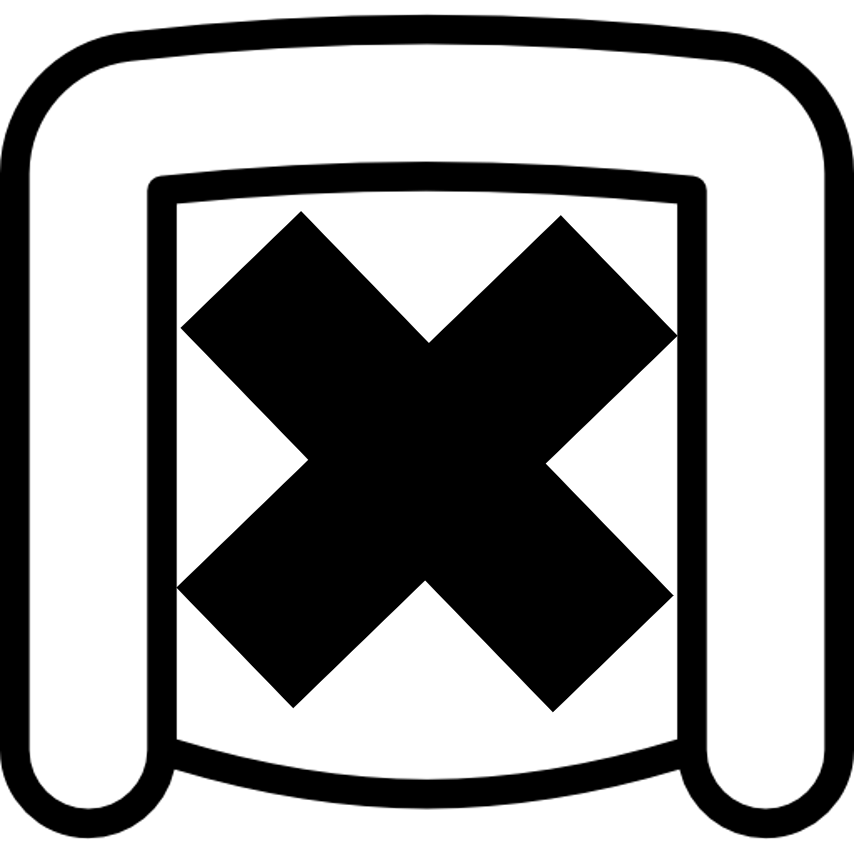
\includegraphics[angle=90, origin=c, scale = 0.09]{Metodologia/visita(x).png}};
        \node (waiting3) [below of = waiting2, yshift = -0.3cm] {
\includegraphics[angle=90, origin=c, scale = 0.09]{Metodologia/visita.png}};
        \node (waitingTexto) [left of = waiting2, rotate = 90, font = \small] {Waiting area};
        
        
        \draw (-5,0) rectangle(5cm,8.5cm);
        
        \draw[arrow] (entry) to ++(0,2.0) to (totem.west);
        \draw[arrow] (totem.north) to ++(0,0.5) to ++(-1.0,0) to (visitor.south);
        \draw[arrow] (visitor.west) to ++ (-3.0,0) to ++(0,-1.0cm) to (waiting3.east);
        \draw[arrow] (waiting3.south) to ++(0,-1.0) to ++(4.0,0) to (exit);  
        
    \end{tikzpicture}
    \caption{Scheduled task of the experiment and their order.}
    \label{fig:task_diagram}
\end{figure}

        
        The goal of these tasks is to engage the user to navigate through the room and see if it is able to draw a mental map of the scene as well as use the information of the obstacles in order to avoid them when needed. Beside theses mains components, there are also some minor distractions that is common to hear at a clinical, such as telephone ringing, keyboard typing, people taking and others. These were put to increase the immersion and to be a distraction as well, otherwise it wouldn't simulate the reality of these scenarios.
    
    \subsection{Tools and methods definition}
        There were three types of human factors' assessment tools that were applied at the experiment:
        \begin{itemize}
            \item Task performance; \\  Measured using the time and the number contacts between the user and the furniture throughout the experiment.
            \item Physiological measures; \\ Measured using and ECG sensor, a GSR sensor and a temperature sensor.
            \item Subjective measures. \\ Measured using a NASA-TLX, a SAGAT Adapted questionnaire and a guidance method evaluation questionnaire.
        \end{itemize}
        The details about each method are explained in the sections \ref{subsec:task_performance}, \ref{subsec:physiological_measures} and \ref{subsec:subjective_measures}.
        
    \subsection{Guidance methods development}
        As said in the last section, three different guidance methods were established to be used in the experiment besides the White Cane:, a haptic belt and a virtual cane.
        \begin{itemize}
            \item A audio guidance method; \\ The audio only guidance method will be straight simple. In the course of the experiment the participant could give two different voice commands:
            \begin{itemize}
                \item  "What is around me?"; \\ The answer of this command was a quickly description of the closest furniture around the user.
                \item  "Where is (something)?". \\ The answer of this command was the direction and distance of something asked by the user.
            \end{itemize}
            Each command was answered by a member of the experiment team accordingly.
            
            \item The haptic belt; \\
            That is a belt that had appended 8 vibration devices that vibrate accordingly to the direction and distance of the closest object around the user. More information on the Haptic Belt ahead at Chapter \ref{ch:cinto}.
            
            \item The virtual cane. \\ 
            This was based on the white cane mechanics, that the user "points" the cane to check near obstacles in the direction of the cane. The virtual cane has a similar function, but instead of connecting the user to the object through the cane, it vibrates when it detects an obstacle in the direction pointed by the user. A VR hand-control was used as canes and the user point's it to where he/she wanted. The algorithm used on the Virtual Cane is in the Appendix \ref{ap:virtual_apend}
        \end{itemize}
    

\section{Tryouts and tests' phase}
\label{sec:tests_phase}
        
        At this phase a few tests were performed to evaluate if the experiment was going as planned and to avoid any unfortunate events or errors during the real experiment. It was expected that changes could be needed to be made before the real experiment and there were a few. It was at this phase that the final dimension of the virtual environment and the physical space were defined.

\section{Experiment}
\label{sec:experiment}
        
        As the proper section name says, this phase is were the proper experiment was made.

After all these phases were completed, the next step was to analyze all the data and elaborate their conclusions. Instead of going to the results and discussions, the next Chapters \ref{ch:cenario} and \ref{ch:cinto} will deepen in the virtual environment development and in the haptic belt development in these order. The Figure \ref{fig:ve_re} show a comparisson between the virtual environment created in Unity3D and the real environment assembled in the CCM's entry hall.

%\begin{figure}[!htb]
    \centering
    \tikzstyle{every node}=[font=\large]
    
    \tikzstyle{task} = [rectangle, rounded corners, minimum width=4cm, minimum height=1.5cm,text centered, draw=black, fill=white!30, text width=3.5cm, font=\large]
    \tikzstyle{phase} = [rectangle, minimum width=4cm, minimum height=1.5cm,text centered, draw=black, fill=white!30, text width=3.5cm, font=\Large]
    \tikzstyle{--} = [black, line width = 2mm]
    \tikzstyle{--red} = [ccmRed, rounded corners, line width = 2mm]
    \tikzstyle{arrow_blue} = [ccmDBlue, rounded corners, line width = 2mm, ->]
    \tikzstyle{arrow_red} = [ccmRed, rounded corners, line width = 2mm, ->]
    
    
    \setlength{\fboxsep}{0pt}%
    \setlength{\fboxrule}{1mm}

    \resizebox{\linewidth}{!}{
    \begin{tikzpicture}[node distance=1cm]
        
        \node (image1) [] {\fbox{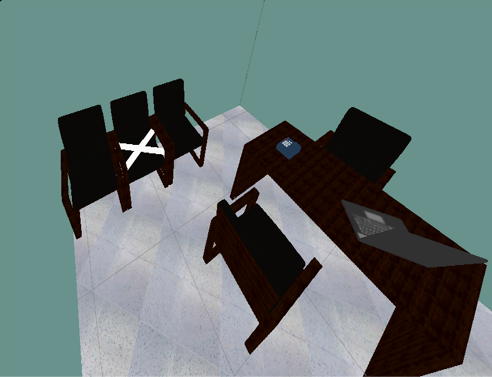
\includegraphics[width = 0.5\linewidth]{Metodologia/VE.png}}};
        \node (image2) [right of = image1, xshift = 7.15cm] {\fbox{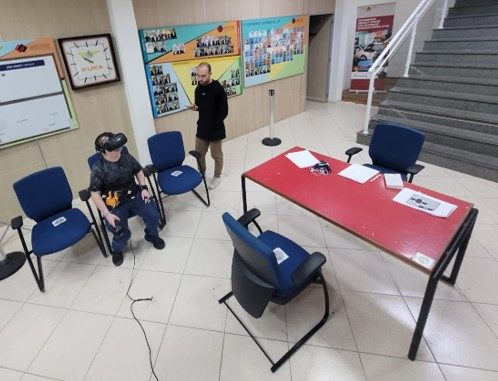
\includegraphics[width = 0.5\linewidth]{Metodologia/RE.jpg}}};

        \node (image3) [below of = image1, yshift = -10cm] {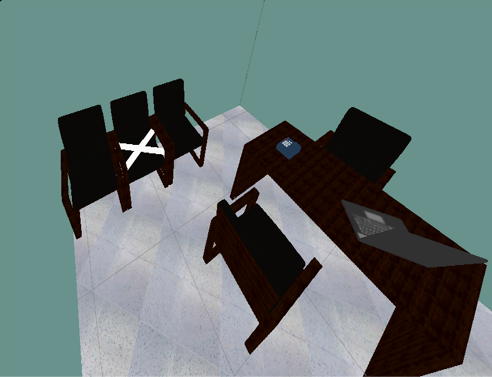
\includegraphics[width = 0.5\linewidth]{Metodologia/VE.png}};
        \node (image4) [right of = image3, xshift = 7.15cm] {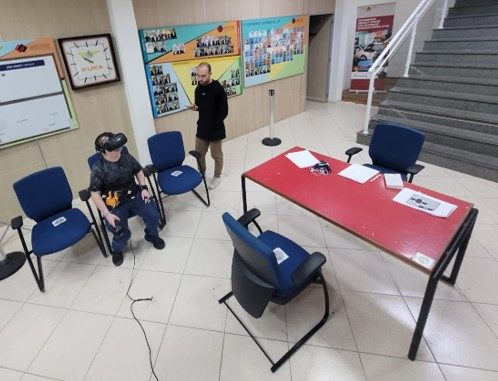
\includegraphics[width = 0.5\linewidth]{Metodologia/RE.jpg}};

        %\node (ponto1) [above of = image1, yshift = 2.5cm, left of = image1, xshift = -3cm] {};
        %\node (ponto2) [above of = image1, yshift = 2.5cm, right of = image1, xshift = 3cm]{};
    
        %\draw[--] (ponto1.west) -- (ponto2.east);
        
    \end{tikzpicture}
    }
    \caption{Virtual and Real environment comparisson}
    \label{fig:ve_re}
\end{figure}

\begin{figure}[!htb]
    \centering
    \begin{subfigure}[b]{0.49\textwidth}
        \centering
        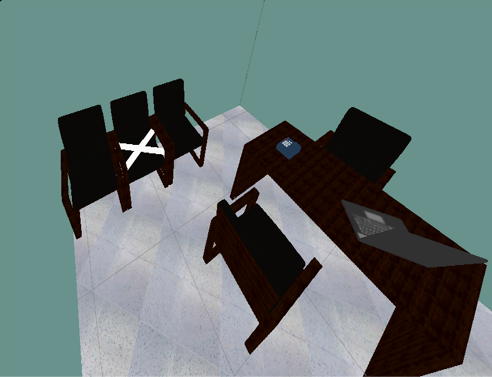
\includegraphics[width=\textwidth]{Metodologia/VE.png}
        \caption{Virtual environment screenshot}
        \label{fig:ve_photo}
    \end{subfigure}
    \hfill
    \begin{subfigure}[b]{0.49\textwidth}
        \centering
        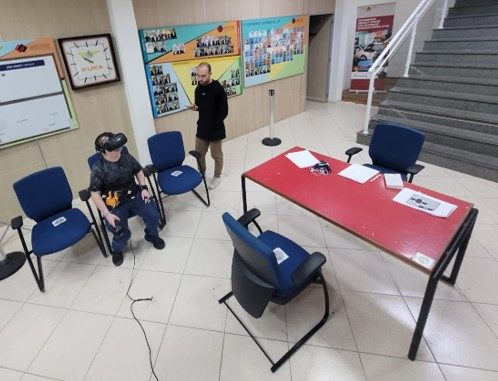
\includegraphics[width=\textwidth]{Metodologia/RE.jpg}
        \caption{Real environment photo}
        \label{fig:re_photo}
    \end{subfigure}
       \caption{Environment comparisson}
       \label{fig:ve_re}
\end{figure}

\chapter{Virtual environment development}
\label{ch:cenario}

The main background and the source of the sensorial input was the virtual environment. Its development can be divided in \ref{itm:final_clinic} steps. The whole procedure is represented in the Figure \ref{fig:ve_process}.

\begin{enumerate}
    \item Procedures
    \item City Hospital
    \item Medical Clinic
    \item Adjustments
    \item Final clinic \label{itm:final_clinic}
\end{enumerate}

\begin{figure}[!htb]
    \centering
    %\tikzstyle{every node}=[font=\large]
    
    \tikzstyle{start} = [rectangle, rounded corners, minimum width=3cm, minimum height=1.0cm,text centered, draw=black, fill=white!30, text width=3cm]
    \tikzstyle{scene} = [rectangle, minimum width=3cm, minimum height=1.0cm, text centered, draw=black, fill=white!30, text width=3cm]
    \tikzstyle{perks} = [diamond, minimum width=1cm, minimum height=1.0cm,  text centered, text width=1.75cm, draw=black, fill=white!30]
    
    \tikzstyle{arrow} = [rounded corners, line width = 1mm, ->]
    \tikzstyle{arrow_blue} = [ccmDBlue, rounded corners, line width = 1mm, ->]
    \tikzstyle{arrow_red} = [ccmRed, rounded corners, line width = 1mm, ->]
    
    \resizebox{\linewidth}{!}{
    \begin{tikzpicture}[node distance=2.5cm]
        \centering
        \node (start) [start] {Hospital procedures};
        \node (city) [scene, below of=start] {City hospital};
        
        \draw [arrow] (start) to node[midway,right]{1st idea} (city);
        
        \node (clinic1) [scene, below of=city] {Medical Clinic V1};
        
        \draw [arrow] (city) to node[midway,right]{Too big} (clinic1);
        
        \node (furniture) [perks, aspect=2.5, below of=clinic1, xshift = -0.5cm, yshift = -0.5cm] {Chairs and desk};
        \node (telephone) [perks, aspect=2.5, right of=furniture, xshift = 2.5cm] {Telephone ringing};
        \node (keyboard) [perks, aspect=2.5, left of=furniture, xshift = -2.5cm] {Keyboard typing};
        
        \draw [arrow_blue] (-0.5cm,-5.5cm) to (furniture);
        \draw [arrow_blue] (-0.5cm,-5.5cm) to ++(0,-1.0cm) to +(-5cm,0) to (keyboard);
        \draw [arrow_blue] (-0.5cm,-5.5cm) to ++(0,-1.0cm) to +(5cm,0) to (telephone);
        
        \node (conv1) [below of = furniture, yshift = 0.5cm] {};
        \node (conv1Texto) [right of = conv1, xshift = -1.0cm] {1st presentation};
        
        \node (tv) [perks, aspect=2.5, below of=conv1, yshift = 0.5cm] {TV playing};
        \node (people) [perks, aspect=2.5, left of=tv, xshift = -2.5cm] {People chatting};
        \node (ticket) [perks, aspect=2.5, right of=tv, xshift = 2.5cm] {Queue machine};
        
        \draw [arrow_blue] (furniture) to (tv);
        \draw [arrow_blue] (keyboard) to ++(0,-1.5cm) to ++(5cm,0) to (conv1) to ++(0,-0.5cm) to ++(-5cm,0) to (people);
        \draw [arrow_blue] (telephone) to ++(0,-1.5cm) to ++(-5cm,0) to (conv1) to ++(0,-0.5cm) to ++(-5cm,0) to (people);
        \draw [arrow_blue] (conv1) to ++(0,-0.5cm) to ++(5cm,0) to (ticket);
        
        \node (clinic2) [scene, right of=ticket, above of = ticket, xshift = 0.5cm, yshift = -0.5cm] {Medical Clinic V2};
        
        \draw [arrow_red] (0.5cm,-5.5cm) to ++(0,-0.5cm) to ++(7.0cm,0) to (clinic2);
        
        \node (clinic3) [scene, right of=ticket, below of = ticket, xshift = 0.5cm] {Medical Clinic V3};
        
        \draw [arrow_red] (clinic2) to (clinic3);
        
        \node (conv2) [below of = tv, yshift = 0.75cm] {};
        
        \node (clinic4) [scene, below of = conv2, xshift = 0.5cm] {Medical Clinic V4};
        
        \draw [arrow_blue] (tv) to ++(0,-3.7cm);
        \draw [arrow_blue] (people) to ++(0,-1.25cm) to ++(5cm,0) to (conv2) to ++(0,-1.95cm);
        \draw [arrow_blue] (ticket) to ++(0,-1.25cm) to ++(-5cm,0) to (conv2) to ++(0,-1.95cm);
        \draw [arrow_red] (clinic3) to node[black,midway,above]{Auditorium complexity} ++(-7.0cm,0) to ++(0,-1.2cm);
        
        \node (exterior) [perks, aspect=2.5, below of=clinic4] {Exterior sounds};
        
        \draw [arrow] (clinic4) to node[midway, right]{1st test} (exterior);
        
        \node (clinic5) [start, below of = exterior] {Medical Clinic V5};
        
        \draw [arrow] (exterior) to (clinic5);
        
    \end{tikzpicture}
    }
        \centering
        \caption{Virtual environment development process}
        \label{fig:ve_process}
\end{figure}

\section{Procedures}

    The first step of the research was to learn how hospitals operate, especially throughout the COVID-19 pandemic. Two hospitals from the city of São José dos Campos - São Paulo were interviewed on how does the reception procedure worked and both of them had a similar operation:
    
    \begin{enumerate}
        \item Patient enters the hospital
        \item Uses the sanitizer to clean their hands
        \item Take a queue number and wait for the call of the receptionist
        \item Go to the receptionist and does his/her check-in
        \item Sits on the waiting area and wait until it's name is called \label{itm:name_call}
    \end{enumerate}
    
    The tasks in the experiment were to be similar to these procedures. The only exception was the name-calling, step \ref{itm:name_call}, because of the complexity of creating a routine inside the virtual environment that could call the participant's name. One possible solution was to use an actor, but because of the COVID-19 procedures that limit the number of people inside a room, this solution was discarded.
    
    Since the procedures were from hospitals, the first idea of a virtual environment was to build a virtual hospital reception.

\section{City Hospital}

    If the virtual environment was a hospital reception, it would be possible to include a lot of artifacts that could increase the participant's sense of presence, such as people walking and the sound of elevators, and that was very appealing.
    
    One problem with that idea was the physical space needed to simulate that. It would be needed a closed-quarters space with enough area to allow the participant to walk through the whole reception. The original space was approximately 15x20m and the laboratory, or the university, didn't have somewhere like that.
    
    So the solution for that was to shrink down the area to fit inside the laboratory, so it was decided not to simulate a hospital reception, but a medical clinic reception

\section{Medical Clinic}

    The laboratory didn't have a room that could fit a hospital reception, but it did have plenty of space that could fit a medical clinic reception, especially in the laboratory's auditorium. The laboratory has 7x10m and that was the dimension of the first version of the virtual medical clinic. At the first moment, it was decided that this would be the setting for the experiment and its development went towards the definition of the interior details (blue path on the Figure \ref{fig:ve_process}), but other problems appeared along with the development that the room dimensions needed to be redefined (red path on the Figure \ref{fig:ve_process}). Both of these modification are going to be detailed in the following \nameref{subsec:interior} and \nameref{subsec:exterior} subsections.
    
    \subsection{Interior}
    \label{subsec:interior}
    
        The goal of the interior was to increase the presence and feeling of the participant inside the virtual environment. The inspiration was from the typical objects and furniture that a patient notices when waiting in reception. The first objects positioned inside the reception were the desk, chairs (both normal and some with "X" in the seats to represent a COVID-19 procedure), a telephone and a laptop. The last two also emitted sounds to increase the feeling of presence and to point to the BVI participant where the reception desk was located. The telephone and the laptop had a C\# script to play their sounds randomly.
        
        This virtual environment was presented to two BVI members of the research team and they pointed out that it needed to have more noise, to increase even more the feeling of presence. They felt the lack of people chattering and the noise that came from a TV show, both were included in the virtual environment. To simulate the people chattering, dialogues from video or series between two people were used. The TV noise was made similarly, but with audio from famous Brazilian tv programs. Another missing artifact noticed by the team was the queue machine that was also included. All these added objects also had a script that played a specific dialogue/program/queue order for each created scene, never repeating once, to increase the sensation of a different day \footnote{During one of the experiments, a BVI participant commented that he/she felt different day times for each time he/she did the scene}. After all of these objects were included, the interior was ready for a trial.
        
    \subsection{Exterior}
    \label{subsec:exterior}
        
        The first version of the clinic had 7x10m, which was the exact dimension of the \textit{Auditório Romi}, the room that was selected to be the physical space for the experiment. Since it was the exact dimension, it became the first change, since an extra space is needed to place the two VR Stations, that in the experiment were assembled on a tripod basis. That modification became the second version of the clinic, with 5x7m.
        
        The second modification came from the maximum distance between the VR Stations. According to "SteamVR" (the software that was the interface between the computer and the VR) the maximum distance was 5m, besides that it could not guarantee the correct operation of the device. Besides that, the auditorium was filled with chairs and without a computer. Every time an experiment was going to be realized, it would be needed to rearrange the entire room, costing almost half an hour to clear the space and another half an hour to return to its place. The solution was to reduce, once more, the virtual environment dimensions to 4x4 and that was the third version of the medical clinic.
        
        The fourth version was reached because, even though smaller, the rearrangement of the auditorium was still a nuisance. The answer to that was to experiment in the entry hall. This was a space, just in front of the room where the computer with all the files was stationed. The only problem was that people passed by until 17h, but since the chosen auditorium was the physical space, it was scheduled that the experiment was going to be performed only during non-working hours.
        
    With these \nameref{subsec:exterior} and \nameref{subsec:interior} modification, the environment was ready to receive its first BVI participant.
        
\section{Adjustments}

    The first BVI participant was the blind member of the research team and he enjoyed the final result, but still found a thing that could help to increase the feeling of presence. He pointed out that BVI people normally find the exit of a room by searching the following sounds in sequence and repeatedly:
    \begin{enumerate}
        \item Sound of a door opening;
        \item Noise from an exterior space (like people walking, cars passing by, horns, etc.);
        \item Sound of a door closing.
    \end{enumerate}
    After that note, a sound-emitting point was added to each environment. This point played this sequence of sounds, but in a random interval.

\section{Final Clinic}

    After that last addition, the clinic reached its final version.




\chapter{Haptic belt development}
\label{ch:cinto}
Since haptic is one of the types of information that a BVI user can rely on, it was a good idea to test haptic devices in the experiment. These haptic devices would not detect the real object per se, but would receive the information from Unity3D based on the position of the user inside the virtual environment.
 
 The virtual cane was a simple development, since the controller already had a vibration motor inside of it. Knowing that, was only a matter to find the right commands and write an algorithm that worked. A pseudo-code is presented at Appendix \ref{ap:virtual_apend}. The two differences between the virtual cane and the haptic belt are the command to check the distance and the fact that with the cane the user must point to the direction where he/she wants to investigate if there is an obstacle whilst the belt indicates to the user the direction of the closest object.
 
 The idea to design a haptic belt came as a suggestion from one of the research members. It was possible to buy one directly from the internet but the cost was too high, so it was decided to assemble one from scratch. The project was based on a haptic compass \cite{kylecorry31_instructables_2020}, but instead of having the input being made by a magnetometer, it was made by the Unity3D.
 
 The first prototype was made using a Arduino Mega 2560, LEDs and a protoboard. If Unity3D could send a command to turn the LED on, then the software would be able to do the same with a coin vibrator. After checking the communication between Unity3D and Arduino, it was time to build the proper belt.
 
 The materials used were:
 \begin{itemize}
     \item DOIT ESP32 DevKit v1. (Datasheet in the Annex \ref{an:esp32_annex});
     \item A printed circuit board (PCB)
     \item A leather belt;
     \item 8 Coin Vibrator 1027;
     \item 16 female P2 jacks or PJ-320B;
     \item 16 P2 male or PJ cable connectors;
     \item 8 straps;
     \item Duct tape;
     \item A 3D printed case.
 \end{itemize}
 
 The first step was to correct and adapt the algorithm used on the Arduino to be used on ESP32 also using the LEDs. After it was made sure that it would also work with an ESP32, the system was designed on the EasyEDA website \cite{easyeda} them a PCB was ordered with the schematic presented in the Appendix \ref{ap:haptic_apend}. While the PCB didn't arrive the coin vibrator and the cables were being soldered. When the PCB arrived, it was time to solder the board P2 jacks and design a case for it, represented in the Figure \ref{fig:case_cinto}. After everything was soldered, printed, and connected it was ready, as is represented in the Figure \ref{fig:cinto_haptico}.
 
 \begin{figure}[!htb]
     \centering
     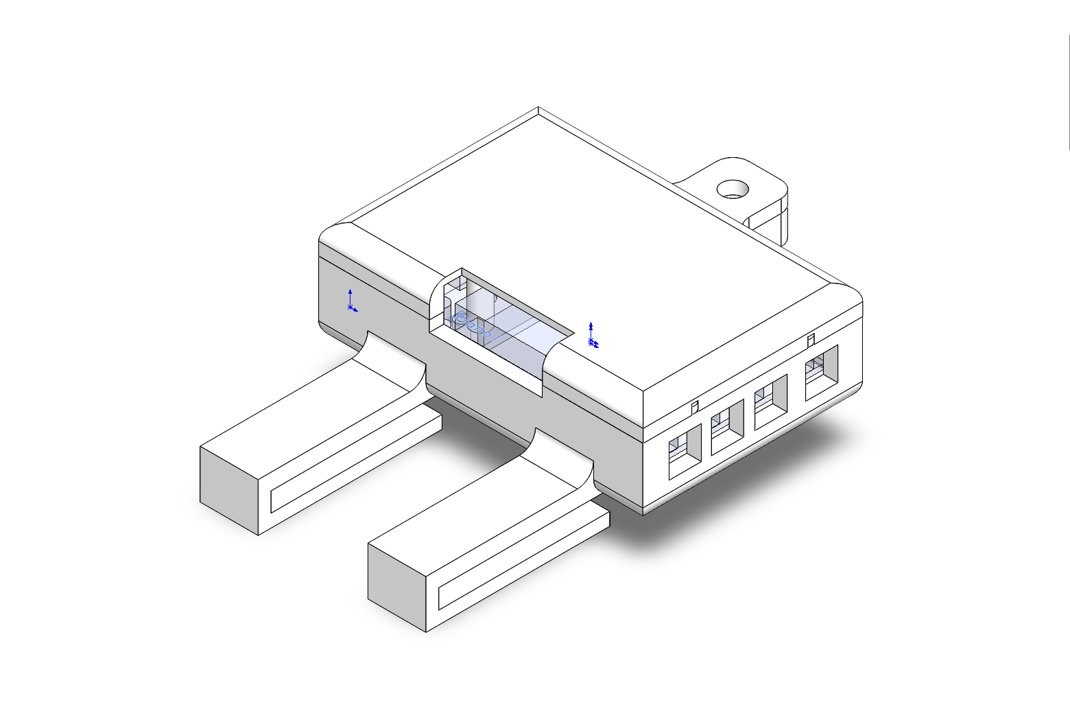
\includegraphics[width = 0.8\linewidth]{Cinto/Case Cinto.png}
     \caption{CAD model of the designed case}
     \label{fig:case_cinto}
 \end{figure}
 \begin{figure}[!htb]
     \centering
     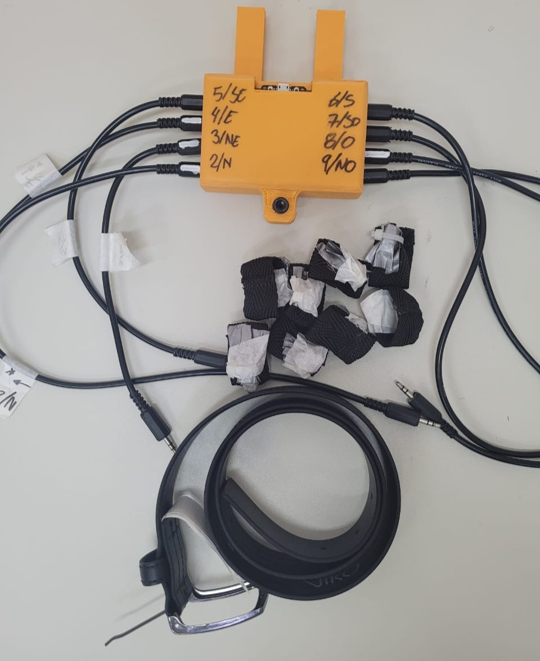
\includegraphics[width = 0.8\linewidth]{Cinto/Cinto Haptico.png}
     \caption{Haptic belt}
     \label{fig:cinto_haptico}
 \end{figure}
 
 Until this moment the belt was working cabled, but since the participant could walk great distances it was decided that the correct way to connect Unity3D with the ESP32 would be by wireless and it was decided to use a Bluetooth connection. The pseudo-code used in the development are in the Appendix \ref{ap:haptic_apend}.


%\chapter{Results' analysis and discussion}
%\label{ch:resultados}
%%CAPÍTULO 4: ANÁLISE DOS RESULTADOS E DISCUSSÃO

%1. Elabore um parágrafo que introduz o capítulo: Este capítulo apresenta (descreva o objetivo do capítulo ...). É constituído de N seções a saber...
%2. Caso vc tenha aplicado a sua contribuição (modelo, produto, processo etc.) em um caso (empresa, laboratório, simulação etc.), apresente a descrição e análise dos resultados. Na seção de discussão cabem as análises de cenários What-If ou de sensibilidade. Exemplo: se o parâmetro X aumentar de N para N+1, o resultado poderia mudar de Y para Z?
%3. Elabore um parágrafo que conclui o capítulo e introduz o capítulo seguinte.

The purpose of the experiment discussed in this chapter is to investigate the two research questions proposed for this work:

\begin{itemize}%[leftmargin = 3.5em, label = $H_\arabic*$:]
    \item Is it possible to evaluate and compare concepts of an assistive device from a human factors' perspective in a virtual environment? What are the main limitations of the use of a virtual reality environment?
    \item Do non-BVI users, when deprived of their vision, similarly evaluate assistive device as BVI users?
\end{itemize}

For this purpose, the experiment described in Section \ref{ch:metodologia} was performed with the following groups:

\begin{itemize}
    \item Blind group: composed of 4 participants with ages varying from 26 to 56, all male, three of them graduated and one with ongoing graduation. 

    \item Sighted group: composed of 4 participants with ages varying from 22 to 31, three males and one woman, all graduated.
\end{itemize}

In order to answer the two research questions, this chapter is organized in the following way. Section \ref{sec:results_obj_1} is dedicated to the first question and brings an analysis performed only with data from blind participants. Then, Section \ref{sec:results_obj_2} repeats the same analysis now with data from sighted participants and compares the results with those obtained from blind participants in order to answer the second research question.

In both sections, the data analysis follows the following sequence:

\begin{itemize}
    \item Analysis of subjective questionnaires:
    \begin{itemize}
        \item NASA-TLX (National Aeronautics and Space Administration Task Load Index): it aims at assessing the workload perceived by the user in six dimensions, including 'mental demand'. It is expected a decrease in the mental workload between the 'first' to the 'return' round. It is also expected that some guidance methods would differ regarding the required mental workload.
        \item Adapted SAGAT (Situation Awareness Global Assessment Technique): it aims at assessing the situation awareness and the user's mental map. It is expected that the SAGAT score would increase from the 'first' to the 'return' round. It is also expected that some guidance methods would differ regarding the required situation awareness provided to the user.
        \item Guidance method's questionnaire: It assess the user experience with each method. It is also expected that some guidance methods would differ regarding the score received in this questionnaire.
    \end{itemize}
    \item Analysis of physiological sensors:
    \begin{itemize}
        \item ECG (Electrocardiogram): it aims at assessing the user workload. Two features are extracted from the ECG signal, heart rate (BPM) and heart rate variance (SDNN). The heart rate is expected to decrease slightly from the 'first' to the 'return' round, while the heart rate variance is expected to increase slightly.
        \item GSR (Galvanic Skin Response): it aims at assessing the user workload and stress. It is expected that the GSR average would increase at every 'first' round and then a slight decrease in the 'return' round.
    \end{itemize}
\end{itemize}

The solution to the collision detection problem would be the acquisition of additional sensors to monitor the user's hands, arms and legs. However, this solution was not feasible within the time frame available for this work. As a result, the performance was removed from the list of factors to be evaluated. Developing an automatic solution for detecting collision in the virtual world is recommended as future work.

Particularly in the case of this work, an additional round of tests is added to the experiment to investigate the differences between the evaluation performed by BVI users and sighted (non-BVI) users. For this purpose, the experiment is repeated with a set of non-BVI users and the same data is collected. The purpose is to investigate whether or not performing the analysis with non-BVI users could lead to different conclusions.

The experiment has an approval of the ethics commitee.


\section{Evaluation of assistive device from a human factors' perspective in a virtual environment}
\label{sec:results_obj_1}

\subsection{Subjective data}
\subsubsection{NASA-TLX}
\label{subsubsec:results_nasa_tlx_1}

The NASA-TLX provides two relevant pieces of information to the workload analysis. The first is the score attributed to the "mental demand" dimension and the second is the average obtained from NASA-TLX's six dimensions. The two analyses are presented in the next subsections.

\paragraph{Analysis of the mental demand scale}\mbox{}\\

Table \ref{tab:md_table_blind} presents the "mental demand" score of each blind participant to each guidance method. The "base" method refers to the guidance method that the person uses in his/her daily life (e.g., white cane). 


\begin{table}[!htb]
\centering
\caption{Score of NASA-TLX mental demand for the blind participants.}
\label{tab:md_table_blind}
\begin{tabular}{llrrrrr}
\toprule
     &        & Base & Audio & \begin{tabular}[c]{@{}l@{}}Haptic\\ Belt\end{tabular} & \begin{tabular}[c]{@{}l@{}}Virtual\\ Cane\end{tabular} & Mixture \\
Participant & Round &      &       &                                                       &                                                        &         \\
\midrule
001C & First &    3 &     1 &                                                    14 &                                                      3 &       6 \\
     & Return &    1 &     1 &                                                    10 &                                                      2 &       6 \\
002C & First &    5 &     1 &                                                     1 &                                                     10 &      12 \\
     & Return &    1 &     1 &                                                     1 &                                                     10 &       3 \\
003C & First &    5 &     5 &                                                     5 &                                                      8 &       1 \\
     & Return &    3 &     1 &                                                     1 &                                                      2 &       1 \\
004C & First &    9 &    10 &                                                    15 &                                                     10 &      10 \\
     & Return &    7 &    10 &                                                    14 &                                                      8 &      10 \\
\bottomrule
\end{tabular}
\end{table}



The mean value obtained for each guidance method is illustrated in Figure \ref{fig:barplot_md_avg_5_scene_blind}. It shows a systematic reduction in the perceived mental workload between the rounds for all methods, confirming that the participants get familiar with the devices after the first use. It also shows that although the haptic belt obtained the most considerable mean, it also had the most significant variation, showing that the effort required from the user may vary significantly.

\begin{figure}[!htb]
    \centering
    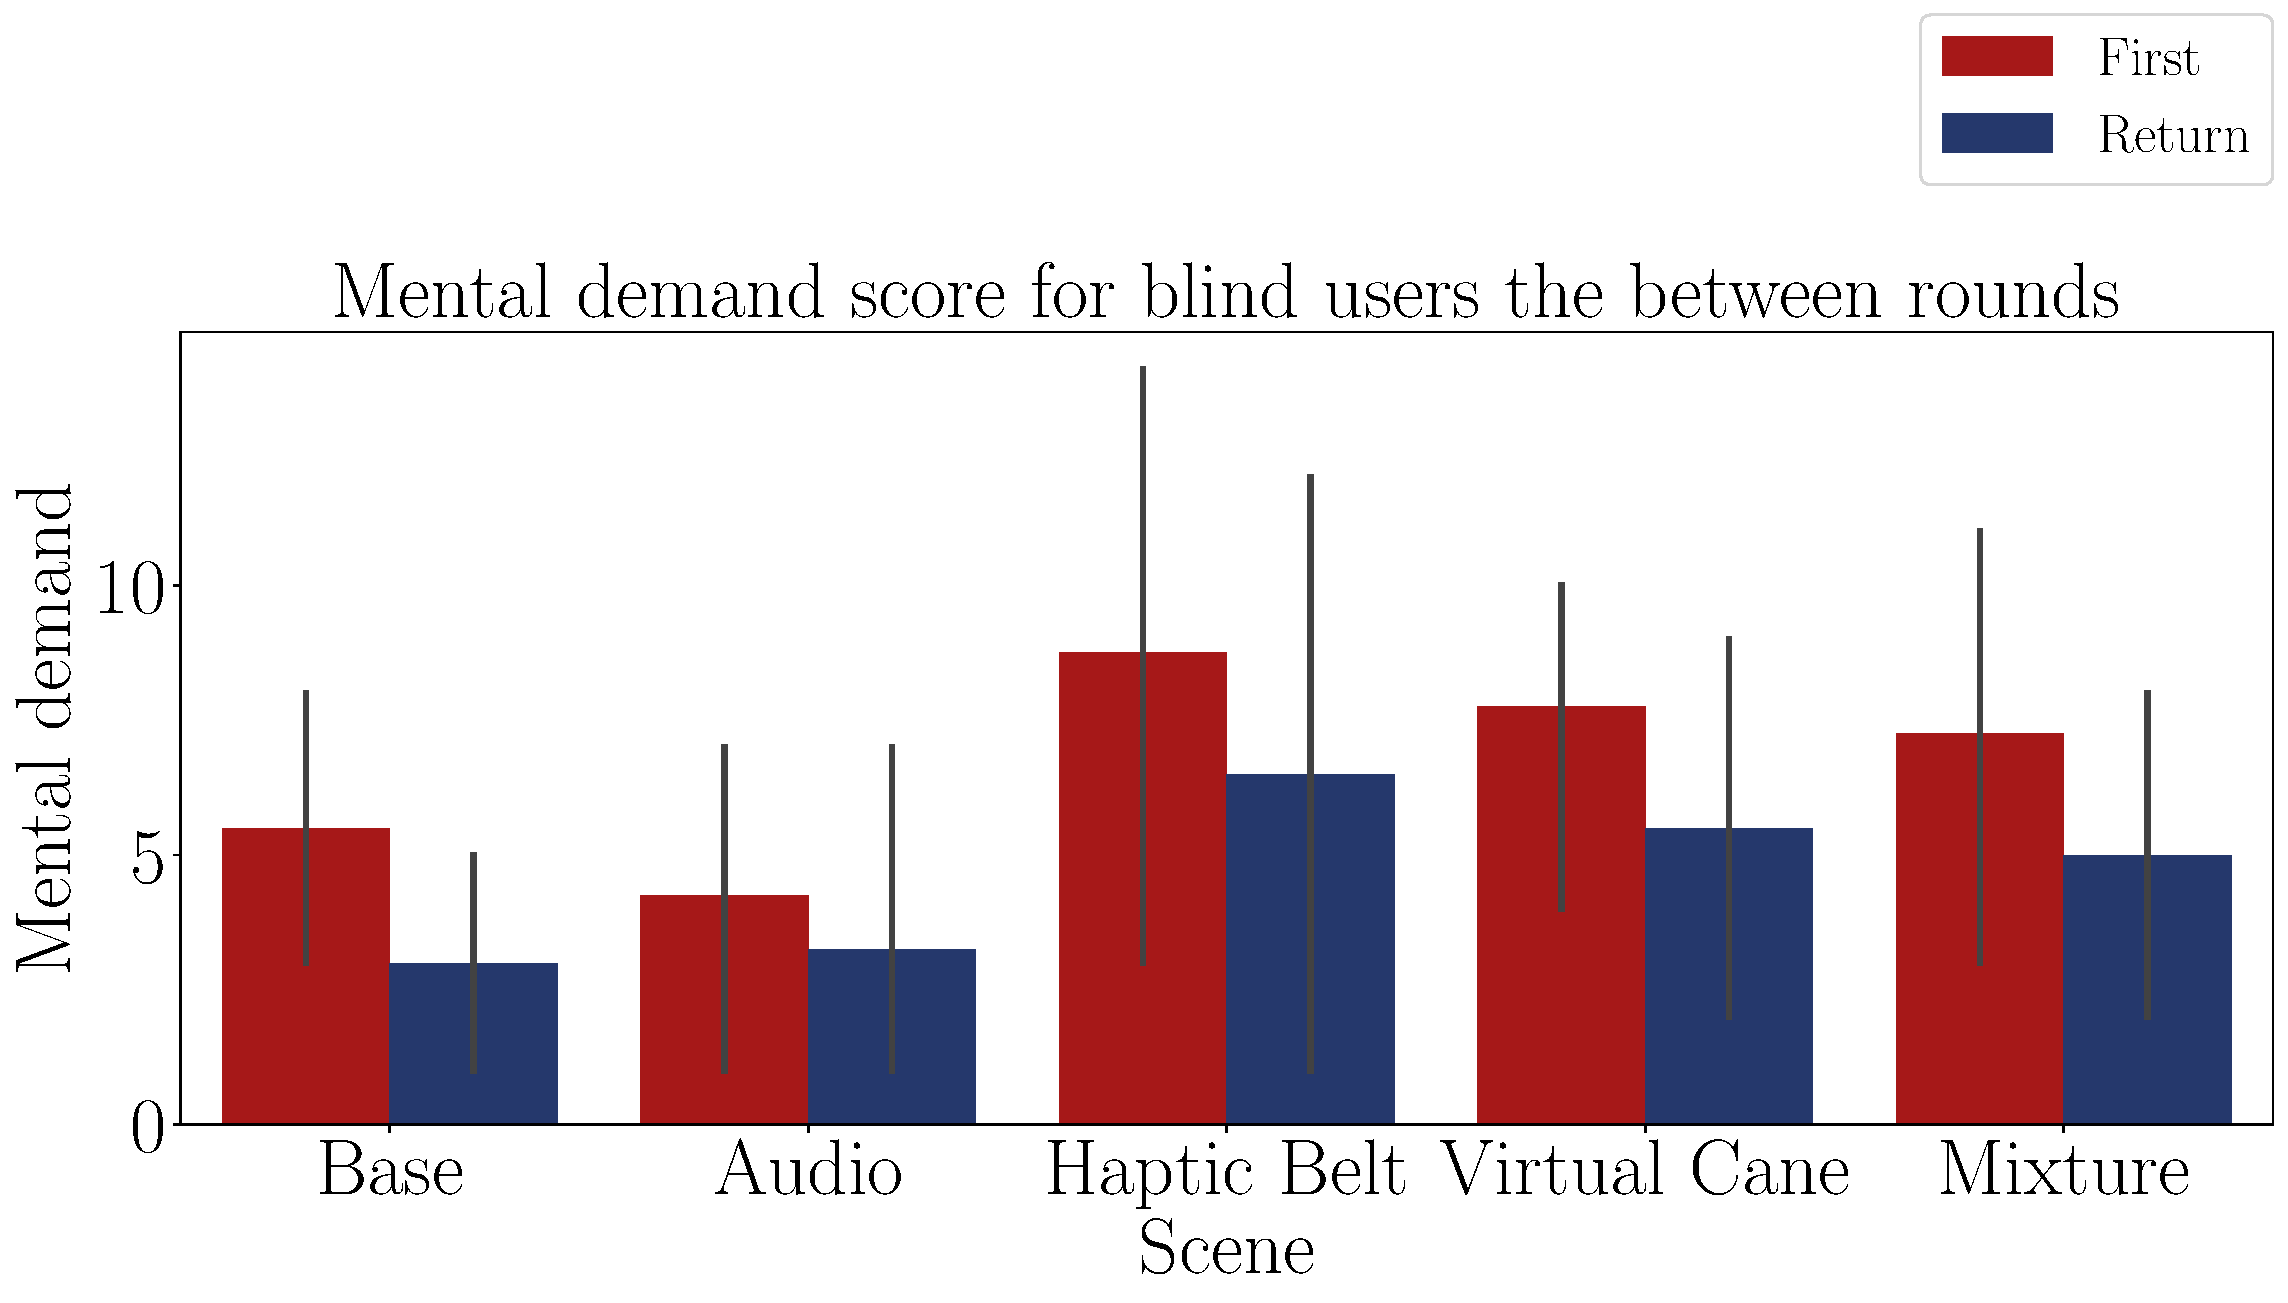
\includegraphics[width = \textwidth]{Resultados/Nasa/Figuras/pdf/barplot_md_avg_5_scene_blind.pdf}
    \caption{Mean and standard deviation of mental demand of blind participants for each method.}
    \label{fig:barplot_md_avg_5_scene_blind}
\end{figure}


Figure \ref{fig:boxplot_md_blind_scene}  presents a boxplot of the mental demand score grouped by the methods. This figure shows that there may be two groups: one associated with lower demand, composed of "base" and "audio", and another with higher demand, composed of "haptic belt", "virtual cane" and "mixture". It indicates that maybe a guidance method that uses vibration as input is not intuitive. Figure \ref{fig:boxplot_md_blind_rounds} presents a boxplot of the mental demand grouped by the rounds, confirming the general tendency to reduce the required "mental demand". 

\begin{figure}[!htb]
    \centering
    \begin{minipage}{0.45\textwidth}
        \centering
        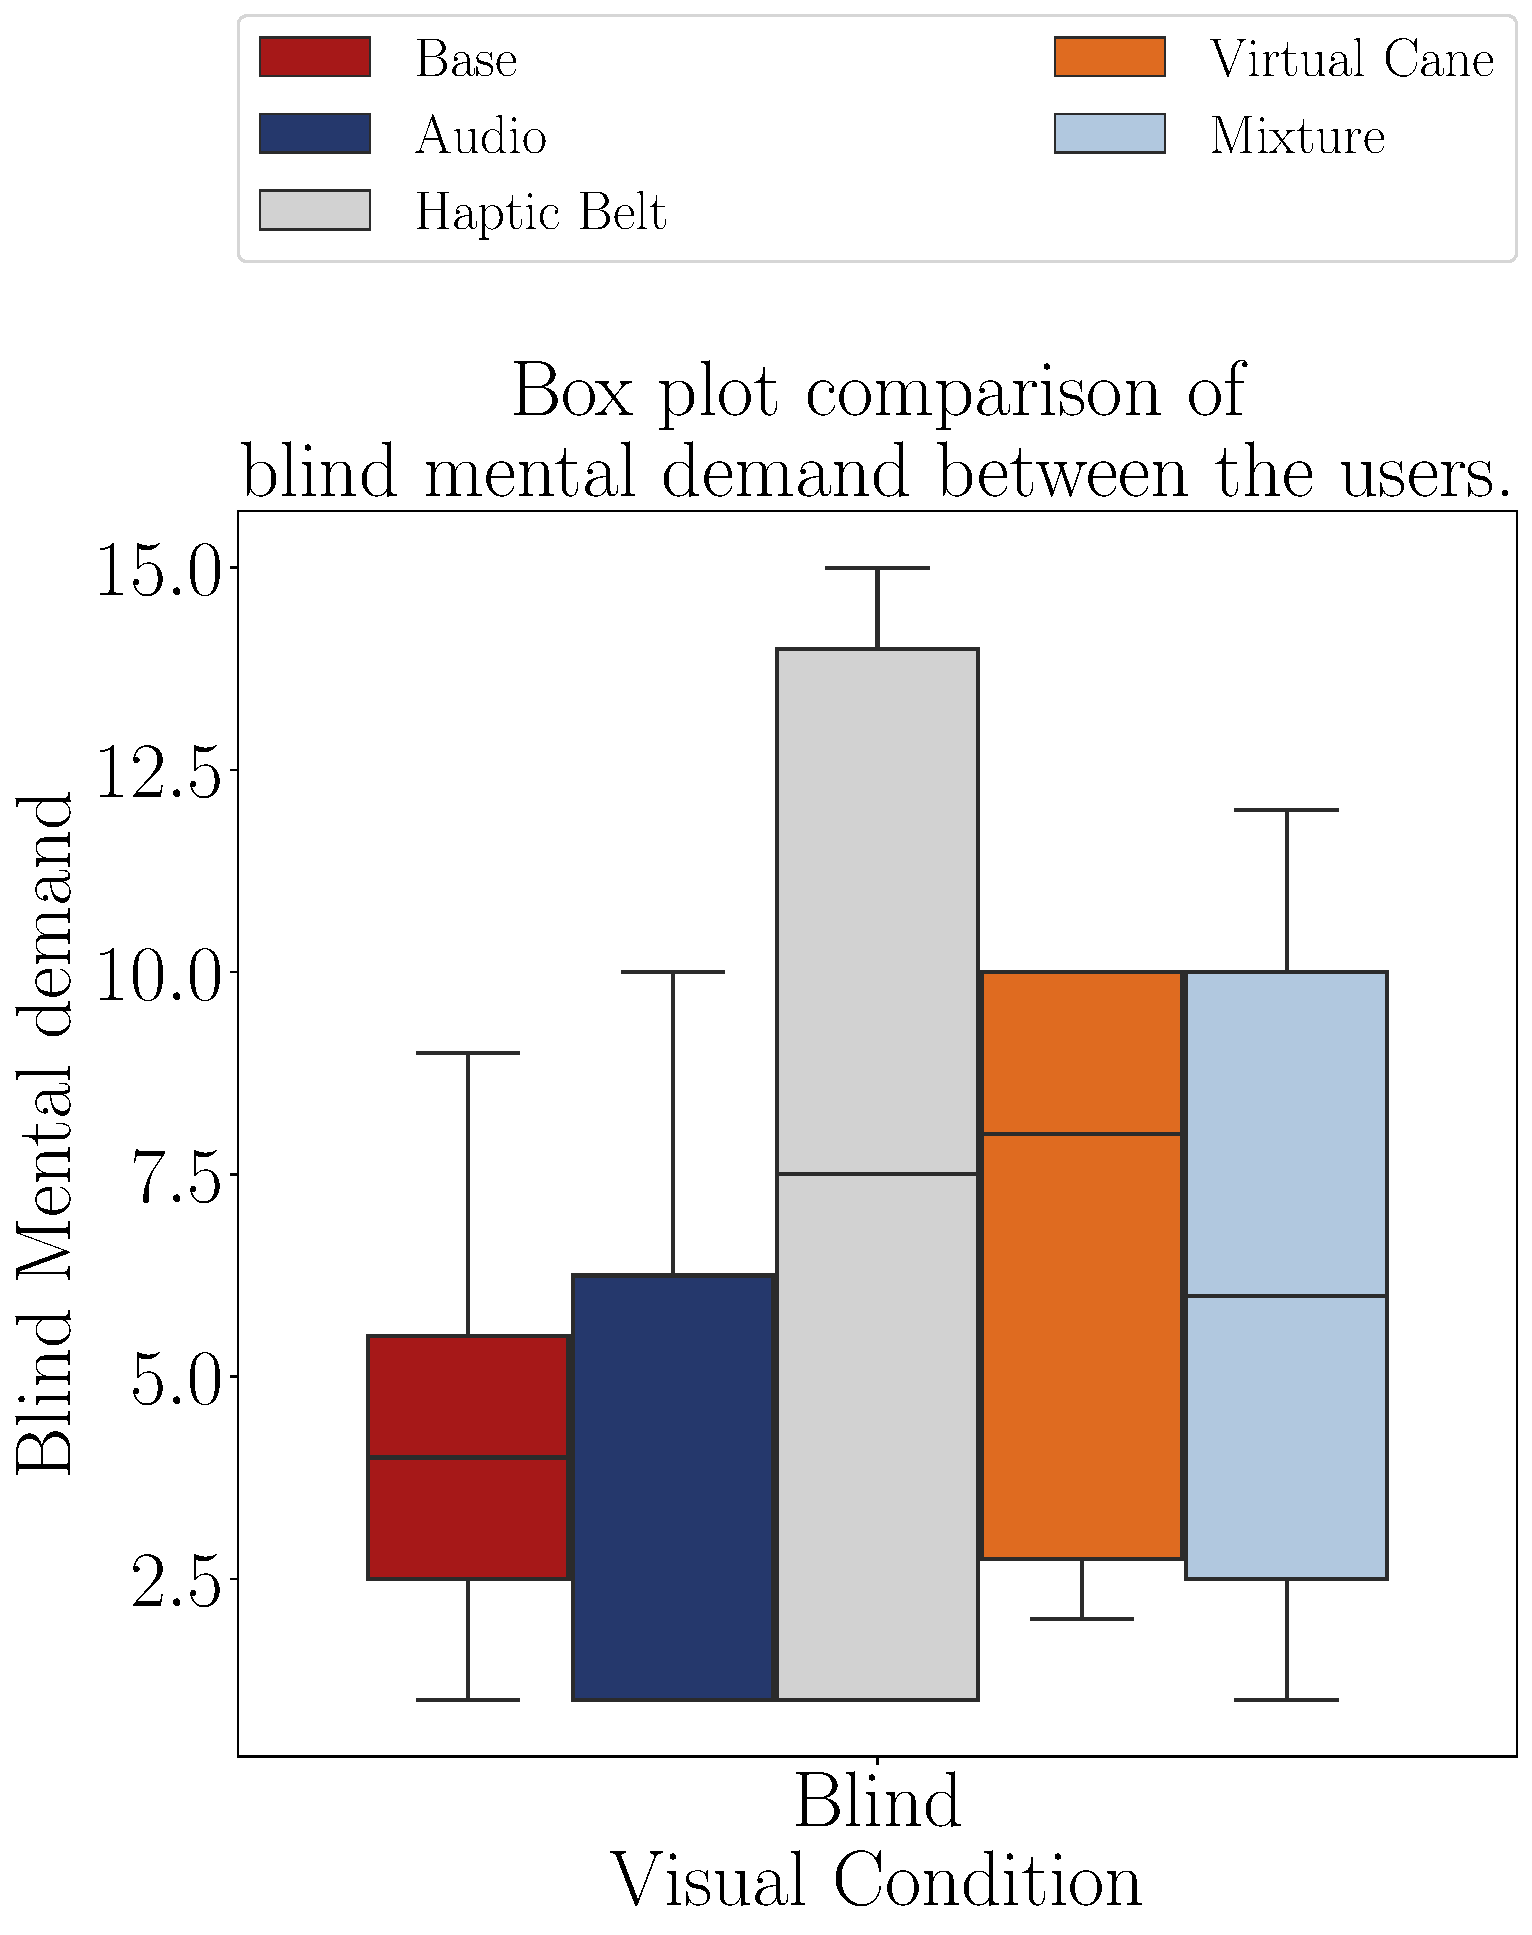
\includegraphics[width = \textwidth]{Resultados/Nasa/Figuras/pdf/boxplot_md_blind_scene.pdf}
        \caption{Boxplot of the mental demand of the blind participants grouped by the methods.}
        \label{fig:boxplot_md_blind_scene}
    \end{minipage}
    \begin{minipage}{0.075\textwidth}
        \hfill
    \end{minipage}
    \begin{minipage}{0.45\textwidth}
        \centering
        %\vspace{3ex}
        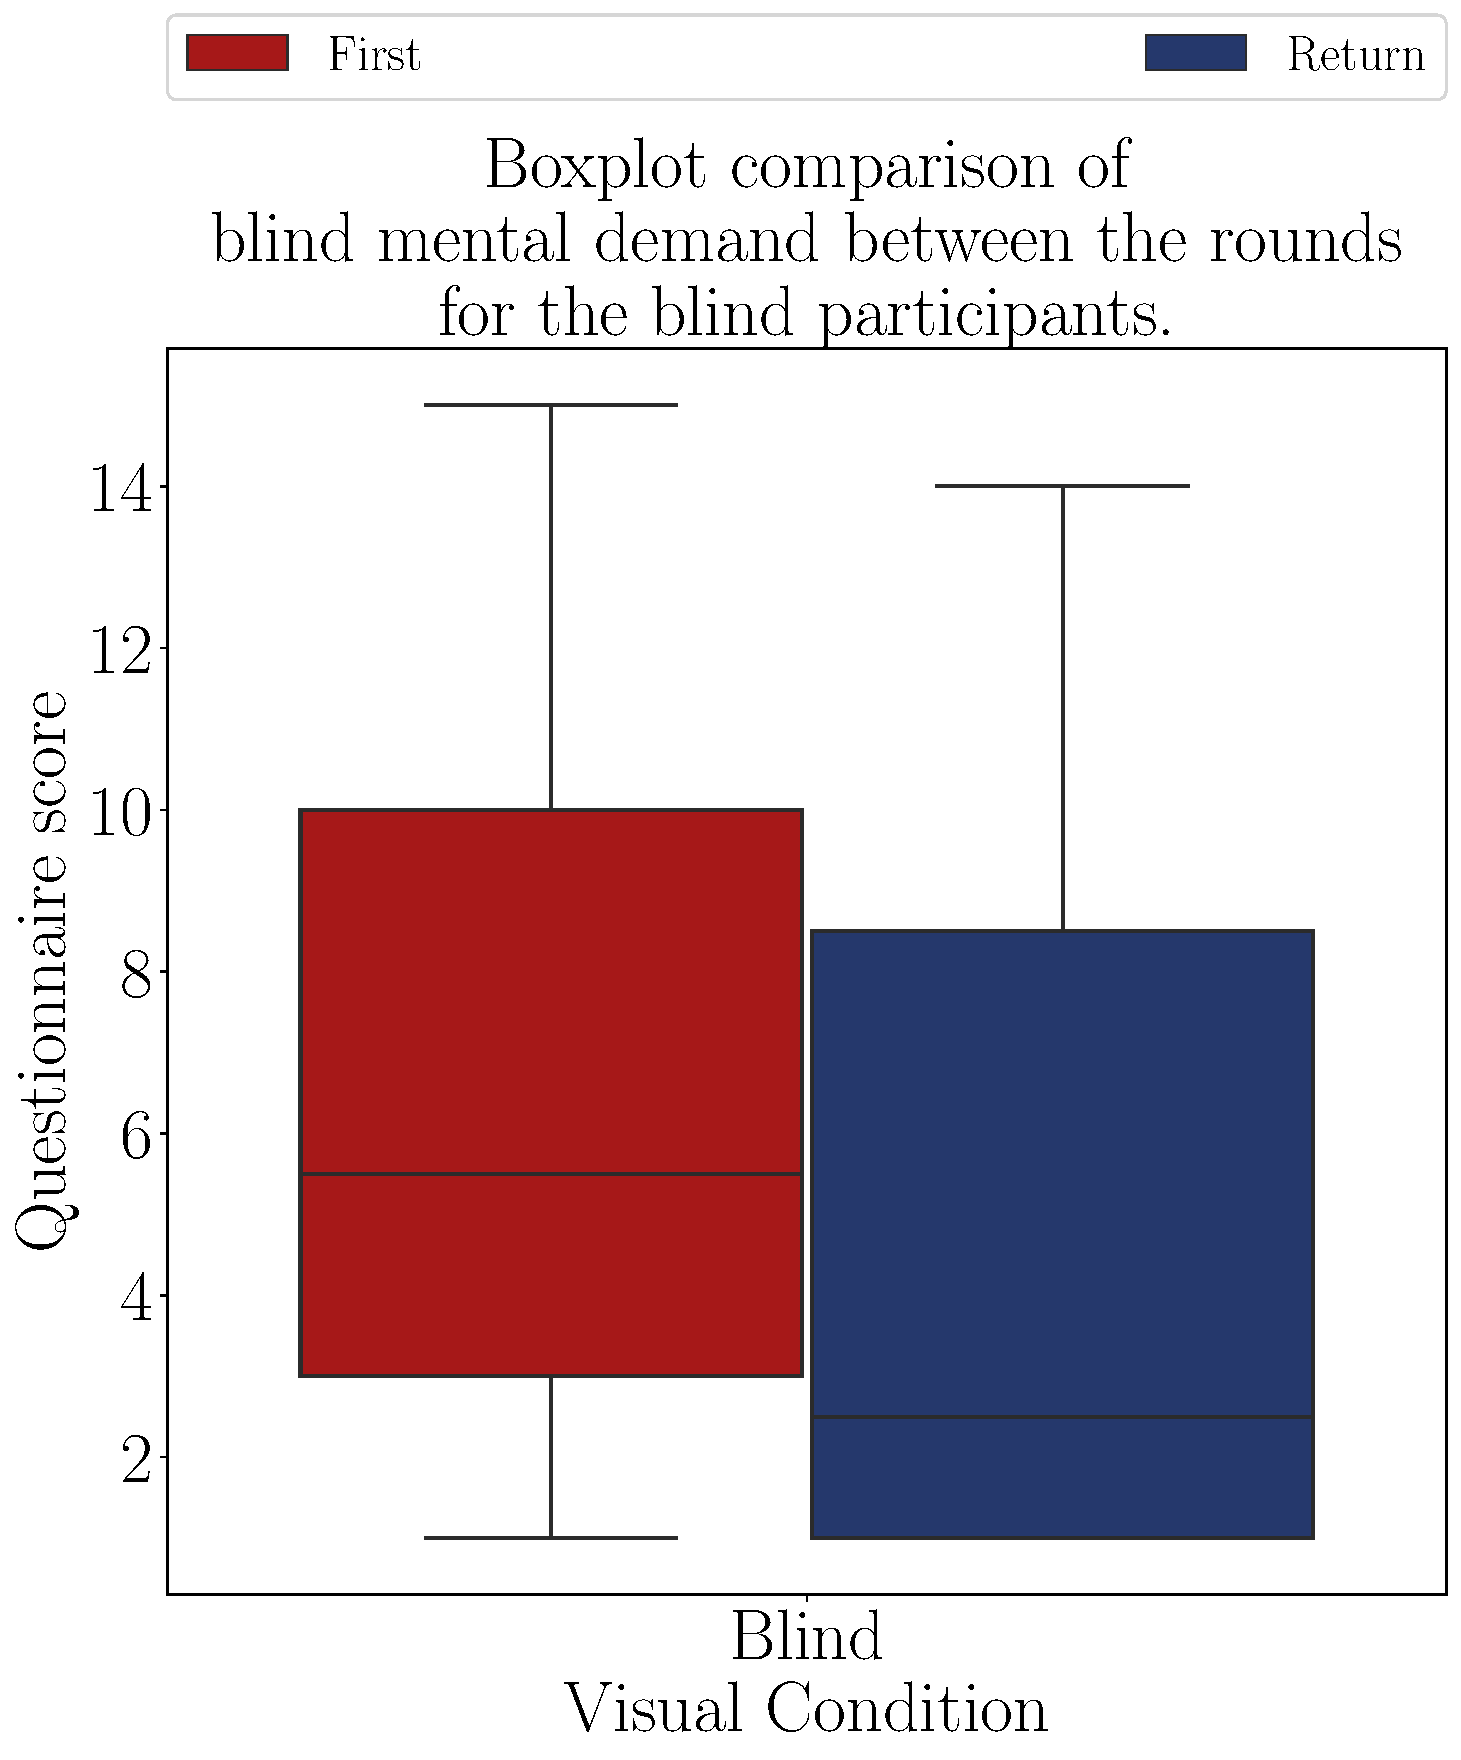
\includegraphics[width = \textwidth]{Resultados/Nasa/Figuras/pdf/boxplot_md_blind_rounds.pdf}
        \caption{Boxplot of the mental demand of the blind participants grouped by the round.}
        \label{fig:boxplot_md_blind_rounds}
    \end{minipage}
\end{figure}

In order to support the statistical analysis, Figures \ref{fig:qqplot_md_avg_two_way_blind} and \ref{fig:residplot_md_avg_two_way_blind} presents the QQ-plot and the residual plot of the "mental demand" data, confirming that the data follow a normal distribution and the residues are homogenous.

Figures \ref{fig:qqplot_md_avg_two_way_blind} and \ref{fig:residplot_md_avg_two_way_blind} show the distribution and variance of Table \ref{tab:md_table_blind}. These figures show that the data are normally distributed and that the methods have a similar variance. Table \ref{tab:blocanova_md_avg_two_way_blind} shows the ANOVA test p-values of the mental demand of the "blind” sample between the guidance methods. The methods' and the rounds' p-values indicate that there is no influence from them in the mental demand. The interaction between the methods and the round also does not influence the mental demand.

\begin{figure}[!htb]
    \centering
    \begin{minipage}{0.45\textwidth}
        \centering
        %\vspace{1ex}
        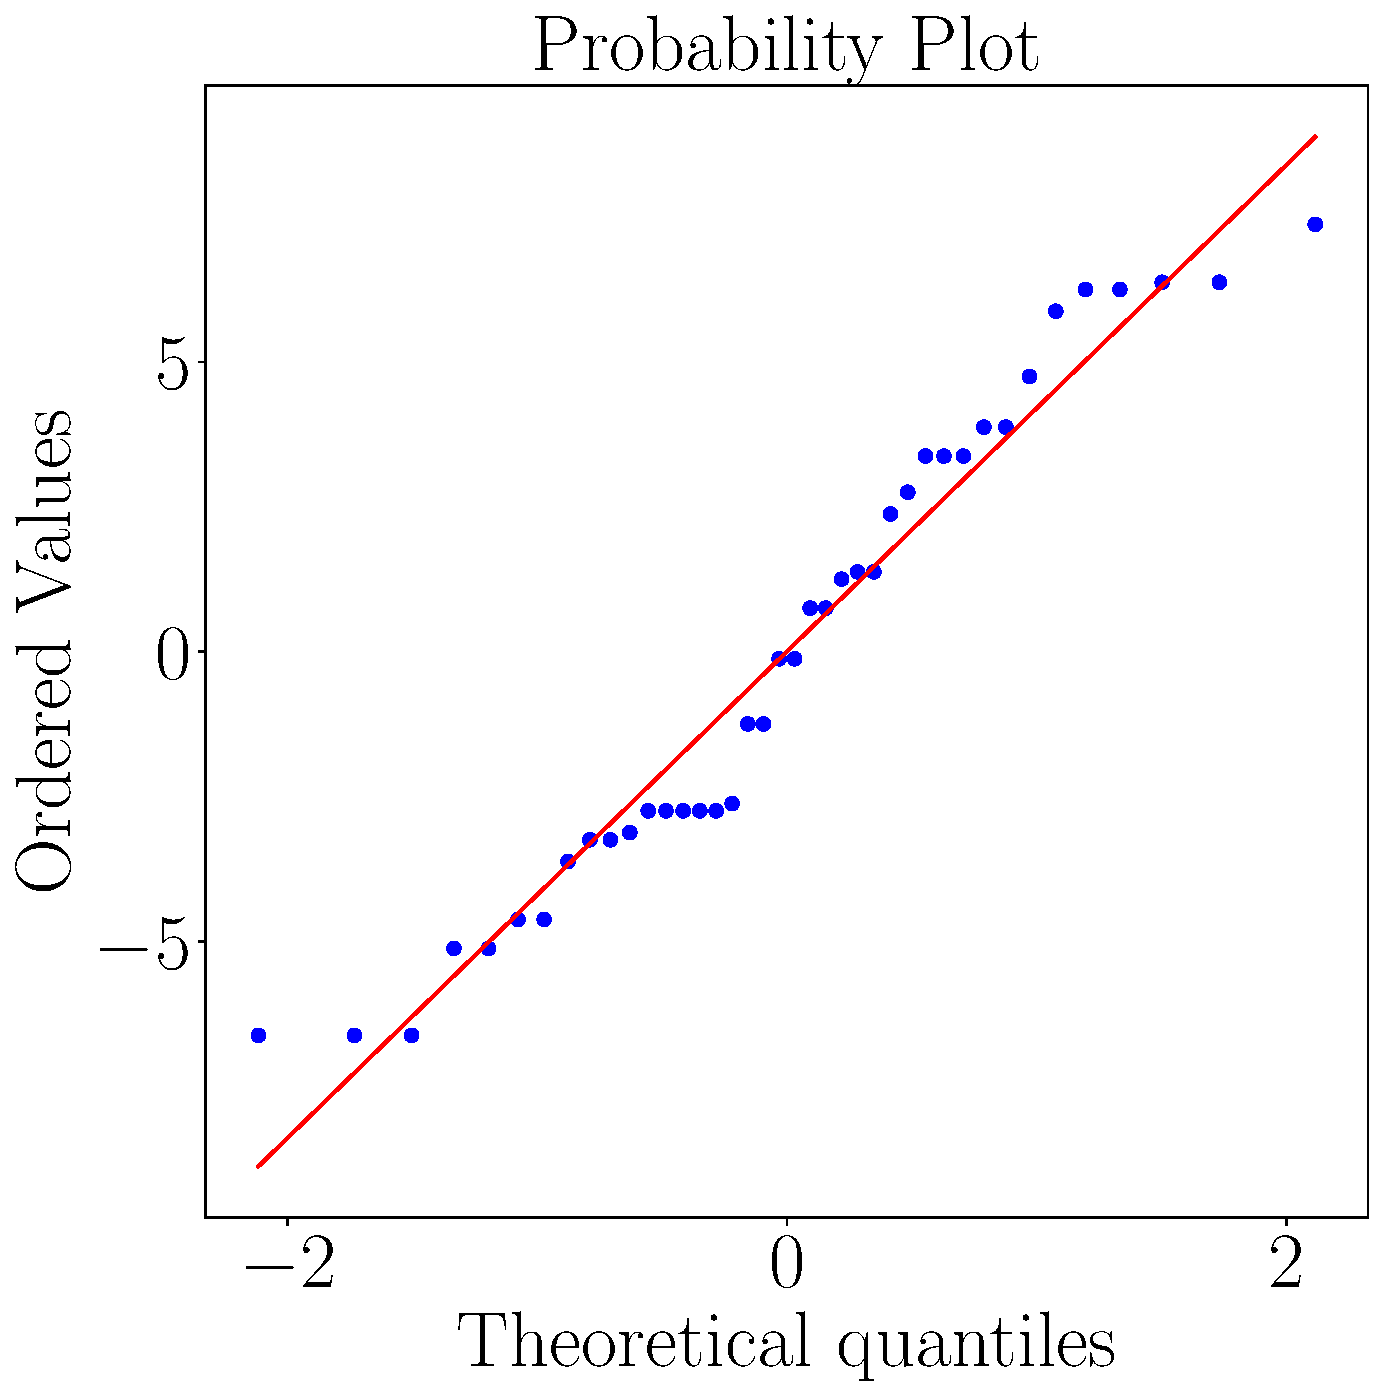
\includegraphics[width = \textwidth]{Resultados/Nasa/Figuras/pdf/qqplot_md_avg_two_way_blind.pdf}
        \caption{QQ plot of the mental demand of the blind participants on each method.}
        \label{fig:qqplot_md_avg_two_way_blind}
    \end{minipage}
    \begin{minipage}{0.075\textwidth}
        \hfill
    \end{minipage}
    \begin{minipage}{0.45\textwidth}
        \centering
        %\vspace{1ex}
        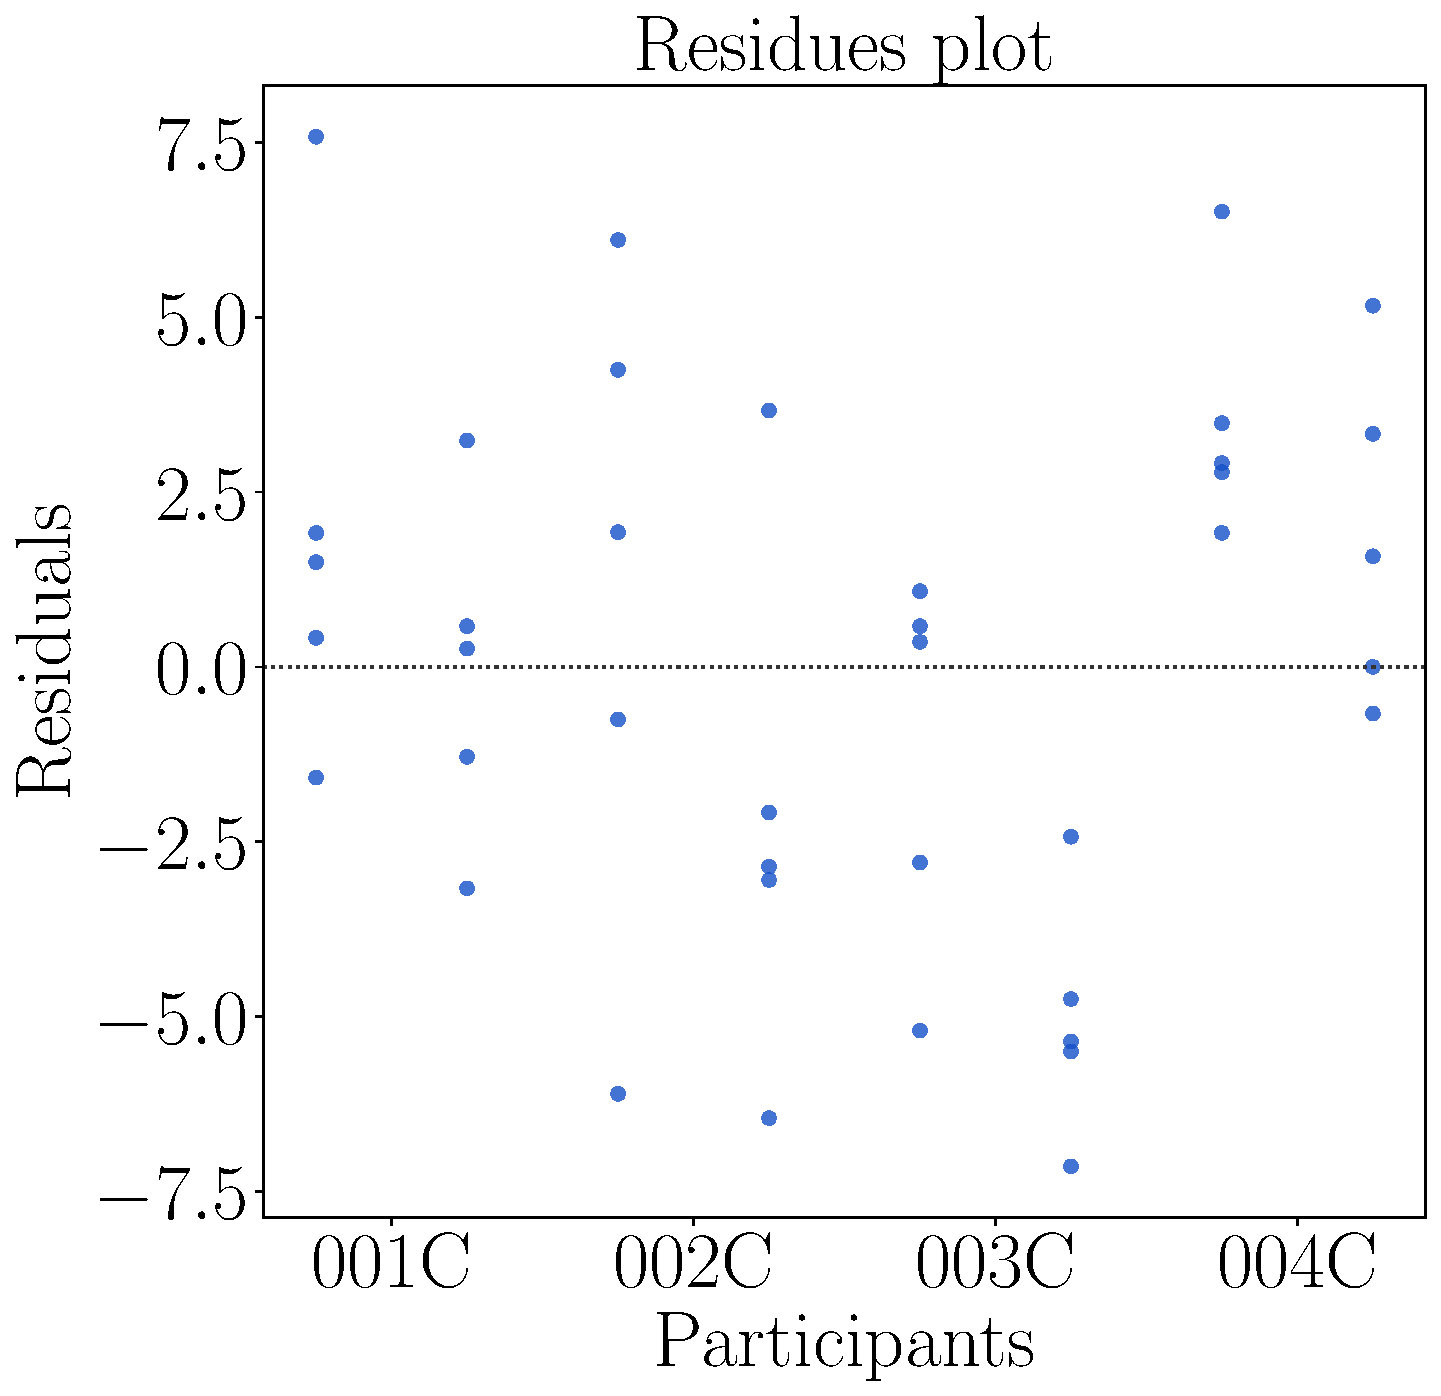
\includegraphics[width = \textwidth]{Resultados/Nasa/Figuras/pdf/residplot_md_avg_two_way_blind.pdf}
        \caption{Residual plot of the mental demand score the blind participants on each method.}
        \label{fig:residplot_md_avg_two_way_blind}
    \end{minipage}
\end{figure}

Following, the statistical model of Equation 5.1 is used for the analysis of variance (ANOVA): 

\begin{equation}
    \label{eq:statistical_model}
    y_{ijk} = \mu + \tau_i + \beta_j + \msout{\omega_k} + (\tau\beta_{ij}) + e
\end{equation}

where:

\begin{itemize}
    \item $y_{ij}$ - output variable for method $i$, round $j$ and participant $k$;
    \item $\mu$ - mean of all the observations;
    \item $\tau_i$ - variance from method $i$;
    \item $\beta_j$ - variance from round $j$;
    \item \sout{$\omega_k$} - variance from participant k, which is treated as a block;
    \item $\tau\beta_{ij}$ - combined variance from the interaction between method i and round j;
    \item $e$ - residual error.
\end{itemize}

The results of ANOVA are presented in Table \ref{tab:blocanova_md_avg_two_way_blind}. ANOVA tests the hypothesis that the means of independent data groups are equal or not. In the literature, a p-value of 0.05 is commonly adopted as a threshold to confirm the hypothesis. A p-value < 0.05 indicates that the means of the groups are statistically different with 95\% of confidence. According to this criterion, neither method or round have a significant influence on the mental demand.

However, due to the low number of participants, the threshold of 0.1 could also be considered. In this case, it indicates, with 90\% confidence, that the mean of the "first" and "return" rounds are different. For the guidance method, the p-value of 0.170 is close to the threshold but slightly higher, suggesting that the means may be different. However, this hypothesis is not statistically confirmed with the current data. 


\begin{table}[!htb]
\centering
\caption{Anova p-value for the mental demand average on each method for blinded users.}
\label{tab:blocanova_md_avg_two_way_blind}
\begin{tabular}{lrrrrl}
\toprule
               Source &  Squared sum &  DOF & Squared average &     F & \begin{tabular}[c]{@{}l@{}}P-Value \\ $(F_{0} > F)$\end{tabular} \\
\midrule
Participants (Blocks) &      298.475 &    3 &          99.492 & 8.133 &                                                                  \\
         \    Methods &       85.150 &    4 &          21.288 & 1.740 &                                                            0.170 \\
          \    Rounds &       42.025 &    1 &          42.025 & 3.436 &                                                            0.075 \\
     \    Interaction &        2.850 &    4 &           0.712 & 0.058 &                                                            0.993 \\
   Experimental Error &      330.275 &   27 &          12.232 &       &                                                                  \\
                Total &      758.775 &   39 &                 &       &                                                                  \\
\bottomrule
\end{tabular}
\end{table}



In order to conclude the analysis of the NASA-TLX mental demand, Table \ref{tab:md_var_average_group_blind} brings the average difference between the mental demand of the "first" and "return" rounds. Unexpectedly, it shows that the most significant variation is obtained to the "base", i.e., the guidance method the participant uses and, therefore, should not present a significant variation. The methods with the lower variation was "audio", probably because it already had a shallow score in the first round. 


\begin{table}[!htb]
\centering
\caption{Mental demand variation grouped by participant and visual condition}
\label{tab:md_var_average_group_blind}
\begin{tabular}{lrrrrrr}
\toprule
{} &  Base & Audio & \begin{tabular}[c]{@{}l@{}}Haptic\\ Belt\end{tabular} & \begin{tabular}[c]{@{}l@{}}Virtual\\ Cane\end{tabular} & Mixture \\
Visual Condition &       &       &                                                       &                                                        &         \\
\midrule
Blind            &  -2.5 &  -1.0 &                                                  -2.2 &                                                   -2.2 &    -2.2 \\
\bottomrule
\end{tabular}
\end{table}



\FloatBarrier

%%%%%%%%%%%%%%%%%%%%%%%%%%%%%%%%%%%%%%%%%%%%%%%%%%%%%%%%%%%%%%%%%%%%%%%%%%%
%%%%%%%%%%%%%%%%%%%%%%%%%%%%%%%%%%%%%%%%%%%%%%%%%%%%%%%%%%%%%%%%%%%%%%%%%%%
%%%%%%%%%%%%%%%%%%%%%%%%%%%%%%%%%%%%%%%%%%%%%%%%%%%%%%%%%%%%%%%%%%%%%%%%%%%
%%%%%%%%%%%%%%%%%%%%%%%%%%%%%%%%%%%%%%%%%%%%%%%%%%%%%%%%%%%%%%%%%%%%%%%%%%%


\paragraph{Analysis of the NASA-TLX score}\mbox{}\\

This section repeats the analysis steps of the previous section but now considers the mean value of all dimensions of NASA-TLX, referred to in this text as the global score. Table \ref{tab:nasa_table_blind} presents the global score of each blind participant. 


\begin{table}[!htb]
\centering
\caption{NASA-TLX score felled by the blinded participants.}
\label{tab:nasa_table_blind}
\begin{tabular}{llrrrrr}
\toprule
     &        &  Base &  Audio & \begin{tabular}[c]{@{}l@{}}Haptic\\ Belt\end{tabular} & \begin{tabular}[c]{@{}l@{}}Virtual\\ Cane\end{tabular} & Mixture \\
Participant & Round &       &        &                                                       &                                                        &         \\
\midrule
001C & First & 4.833 &  4.000 &                                                 8.833 &                                                  5.167 &   6.333 \\
     & Return & 4.167 &  4.000 &                                                 6.667 &                                                  4.500 &   6.167 \\
002C & First & 6.333 &  4.833 &                                                 4.833 &                                                  9.000 &   7.000 \\
     & Return & 4.500 &  4.833 &                                                 4.833 &                                                  7.000 &   5.167 \\
003C & First & 4.000 &  4.000 &                                                 5.333 &                                                  6.667 &   3.500 \\
     & Return & 4.000 &  3.833 &                                                 3.667 &                                                  3.500 &   3.500 \\
004C & First & 9.833 & 10.000 &                                                12.667 &                                                  9.667 &  11.000 \\
     & Return & 8.667 &  9.167 &                                                11.667 &                                                  9.333 &  10.833 \\
\bottomrule
\end{tabular}
\end{table}



Figure \ref{fig:barplot_nasa_avg_5_scene_blind} brings the corresponding barplot with the mean value and standard deviation for each guidance method and each round. In a qualitative comparison with Figure \ref{fig:barplot_md_avg_5_scene_blind}, the differences between the methods are confirmed but softened. It is possible to notice that the mean score of "audio" and "base" are still lower than that of the other methods. The differences between "first" and "return" rounds are also reduced. However, the standard deviation is also considerably reduced for all methods, and especially for the haptic belt.

\begin{figure}[!htb]
    \centering
    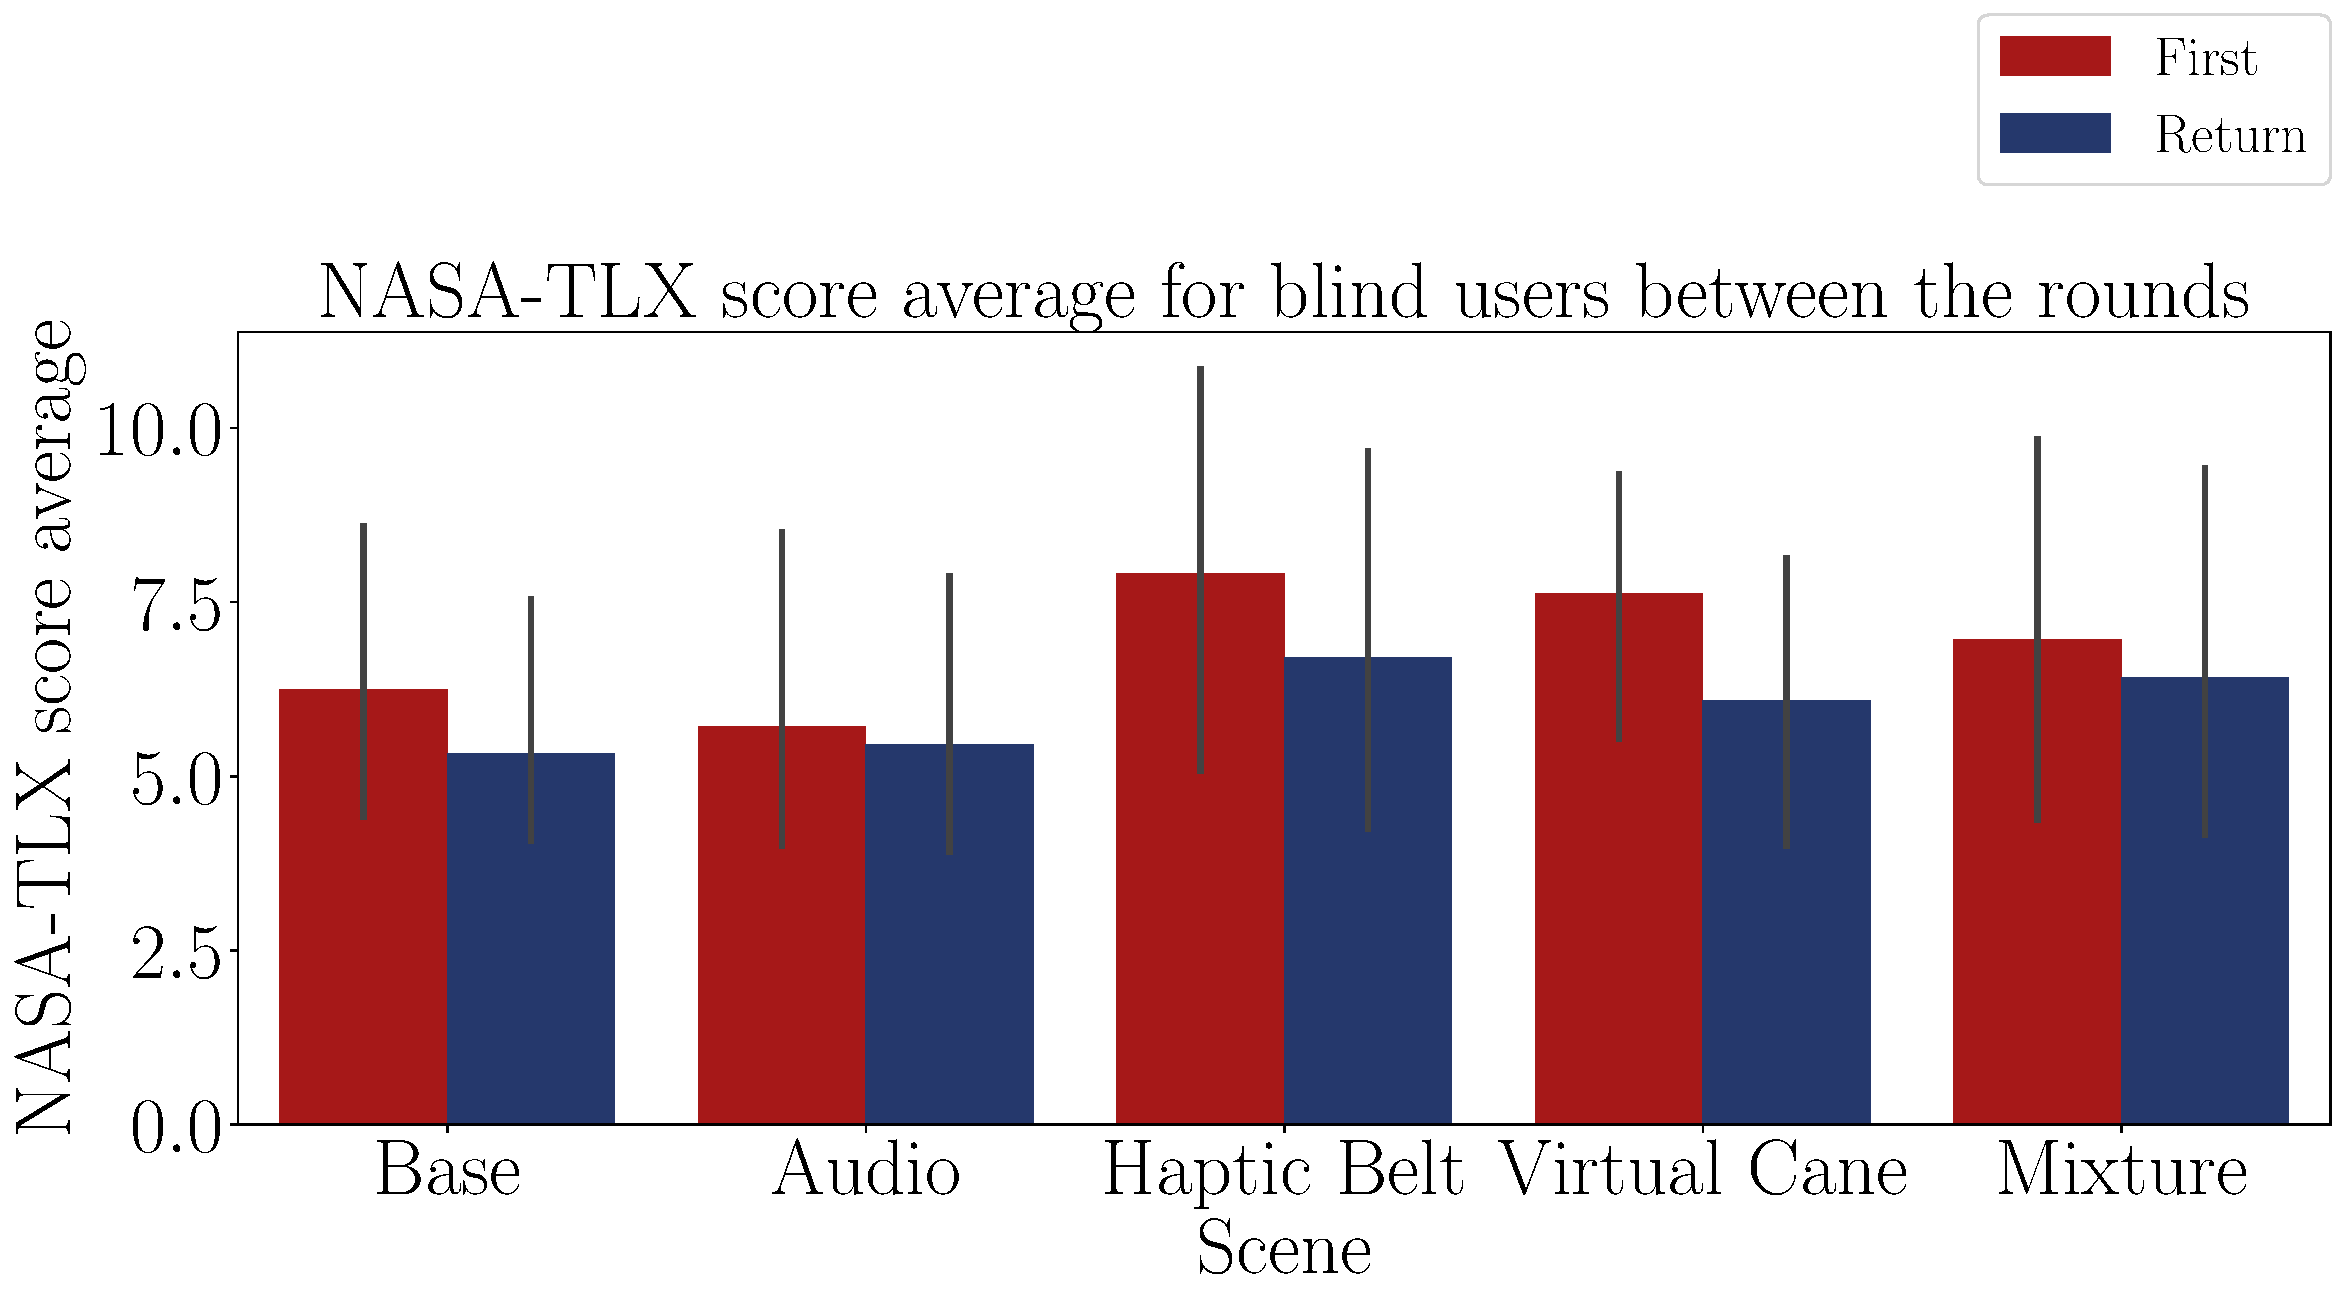
\includegraphics[width = \textwidth]{Resultados/Nasa/Figuras/pdf/barplot_nasa_avg_5_scene_blind.pdf}
    \caption{Barplot of the average NASA-TLX score of the blind participants on each method.}
    \label{fig:barplot_nasa_avg_5_scene_blind}
\end{figure}

Figure \ref{fig:boxplot_nasa_blind_scene} presents the boxplot with the NASA-TLX global score grouped by the methods. Similar to what happened for the "mental demand", it is possible to split the methods into two different groups: "base" and "audio", which require a lower level of workload, and another group, which requires a higher level. Figure \ref{fig:boxplot_nasa_blind_rounds} presents a boxplot with the NASA-TLX global score grouped by the rounds, showing that the two groups are still different. 

\begin{figure}[!htb]
    \centering
    \begin{minipage}{0.45\textwidth}
        \centering
        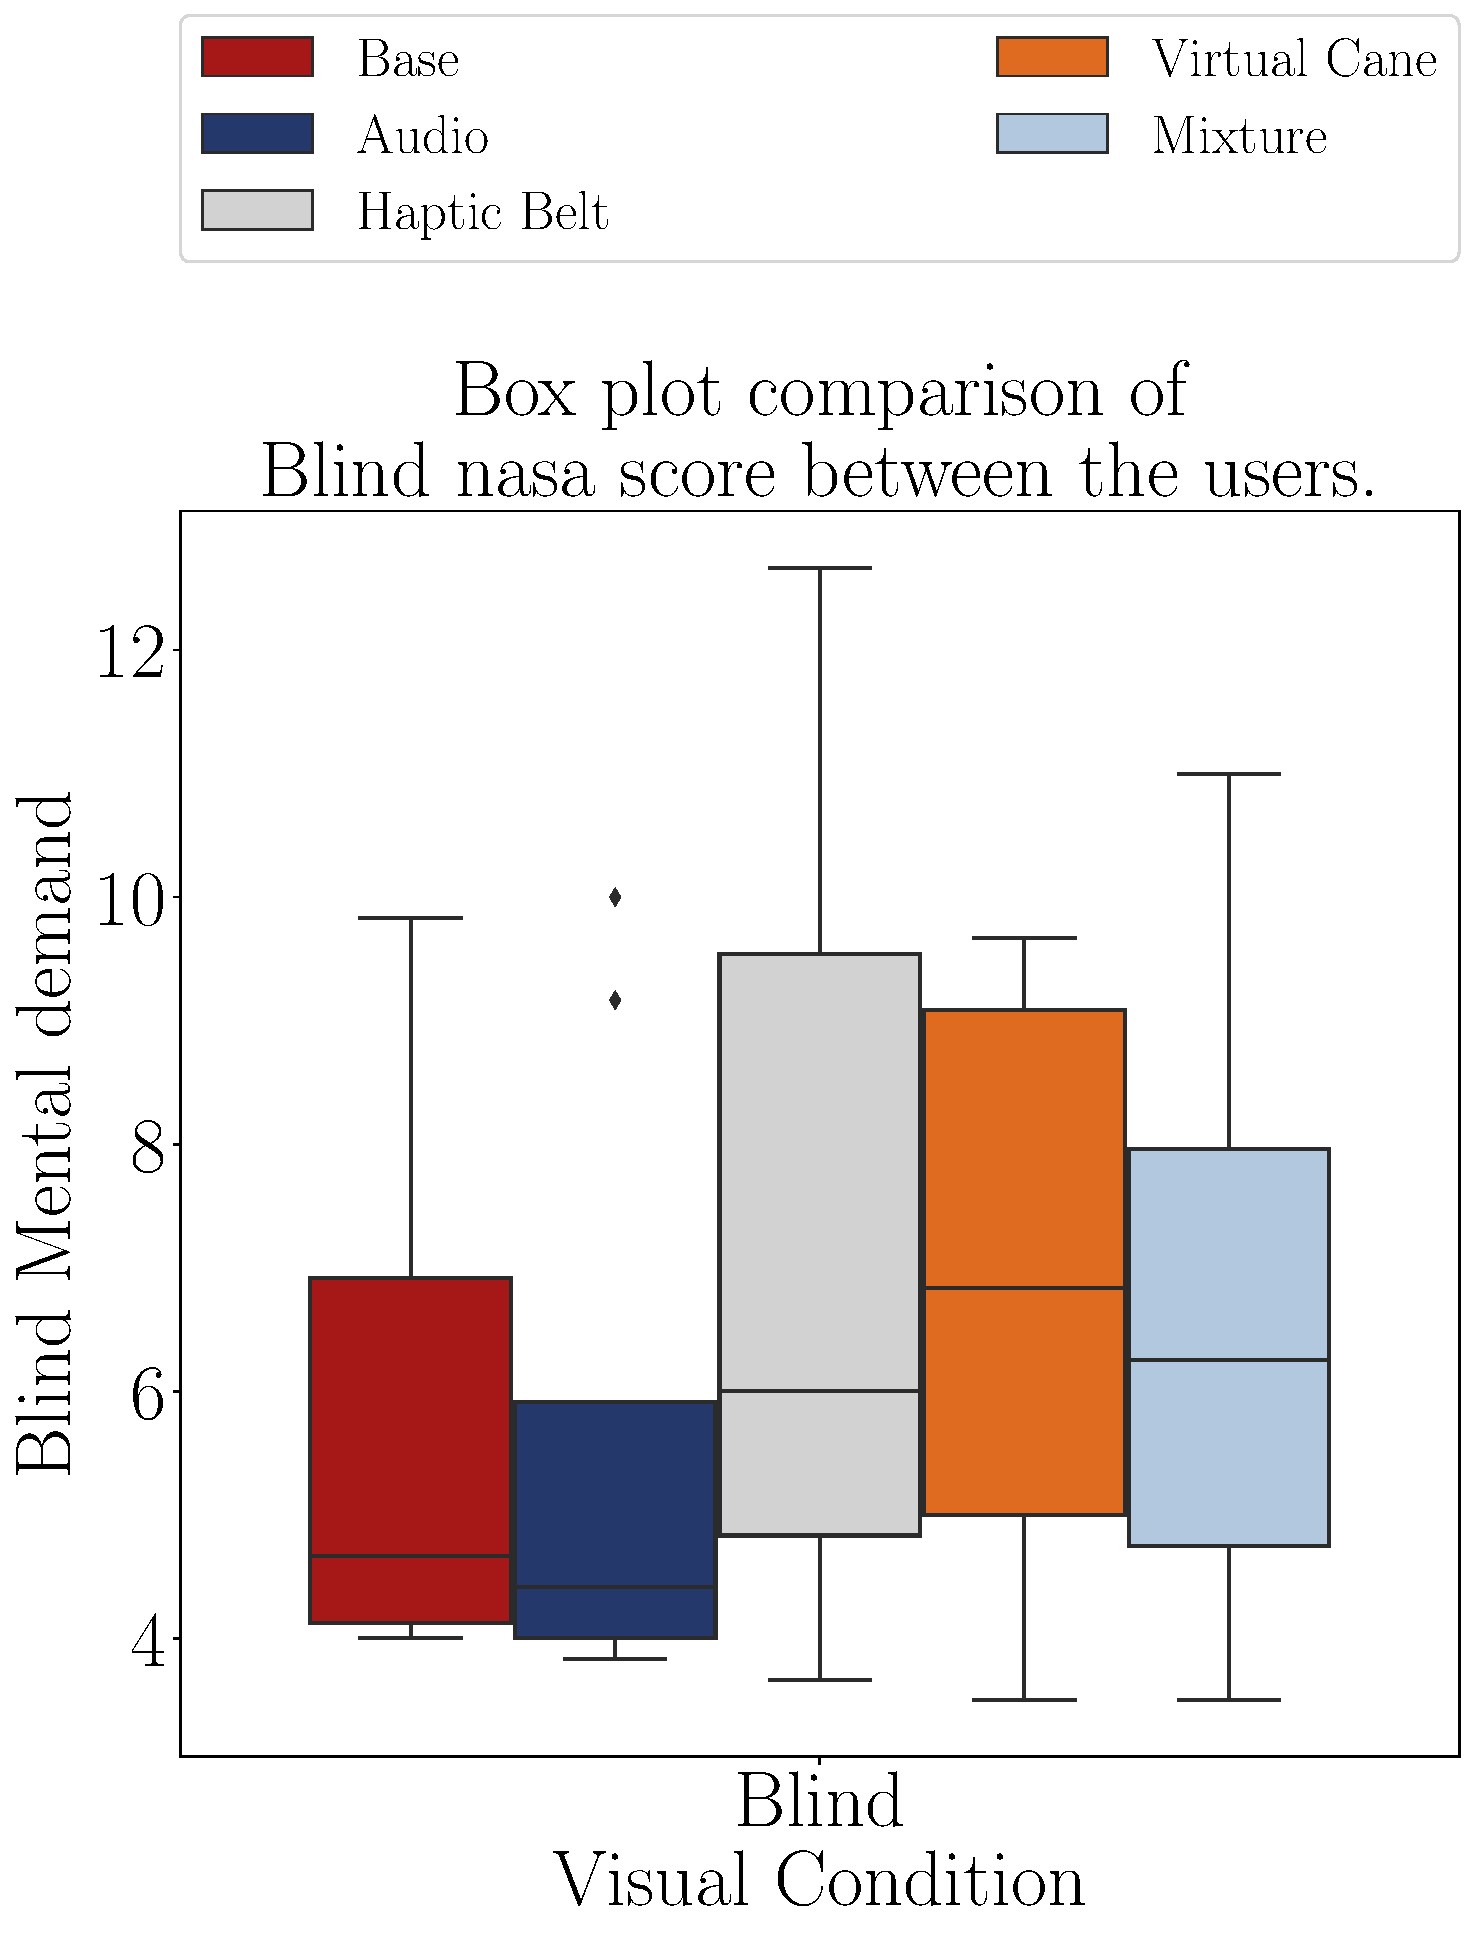
\includegraphics[width = \textwidth]{Resultados/Nasa/Figuras/pdf/boxplot_nasa_blind_scene.pdf}
        \caption{Boxplot of the NASA-TLX of the blind participants grouped by the methods.}
        \label{fig:boxplot_nasa_blind_scene}
    \end{minipage}
    \begin{minipage}{0.075\textwidth}
        \hfill
    \end{minipage}
    \begin{minipage}{0.45\textwidth}
        \centering
        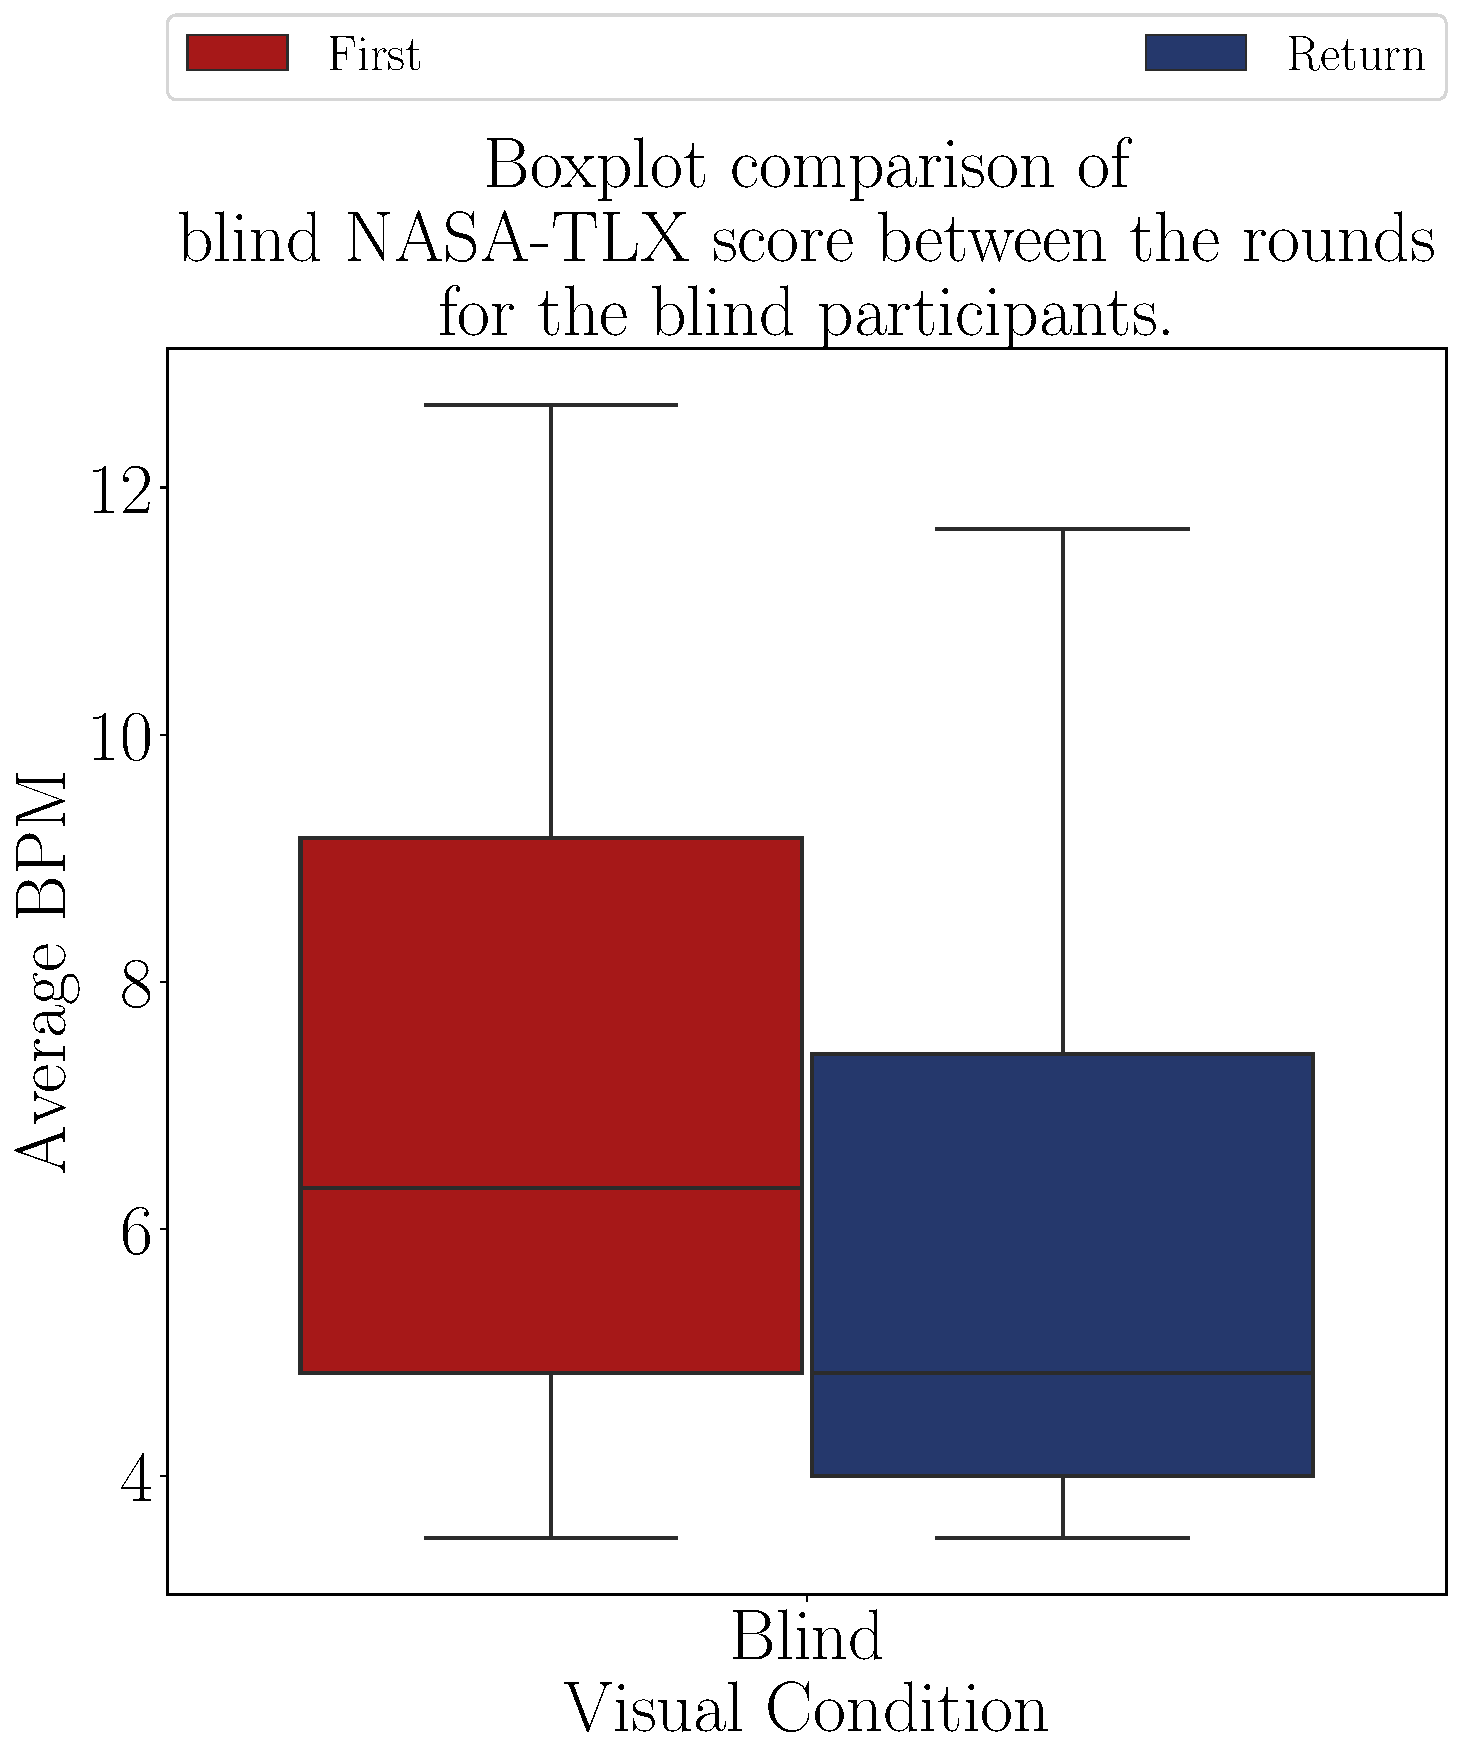
\includegraphics[width = \textwidth]{Resultados/Nasa/Figuras/pdf/boxplot_nasa_blind_rounds.pdf}
        \caption{Boxplot of the NASA-TLX demand of the blind participants grouped by the round.}
        \label{fig:boxplot_nasa_blind_rounds}
    \end{minipage}
\end{figure}

Figures \ref{fig:qqplot_nasa_avg_two_way_blind} and \ref{fig:residplot_nasa_avg_two_way_blind} presents the QQ plot and residual distribution of the NASA-TLX global score, showing that the data are normally distributed. However, the residuals are not so homogeneous as in the previous case, showing that the participants have different variability among them.

\begin{figure}[!htb]
    \centering
    \begin{minipage}{0.45\textwidth}
        \centering
        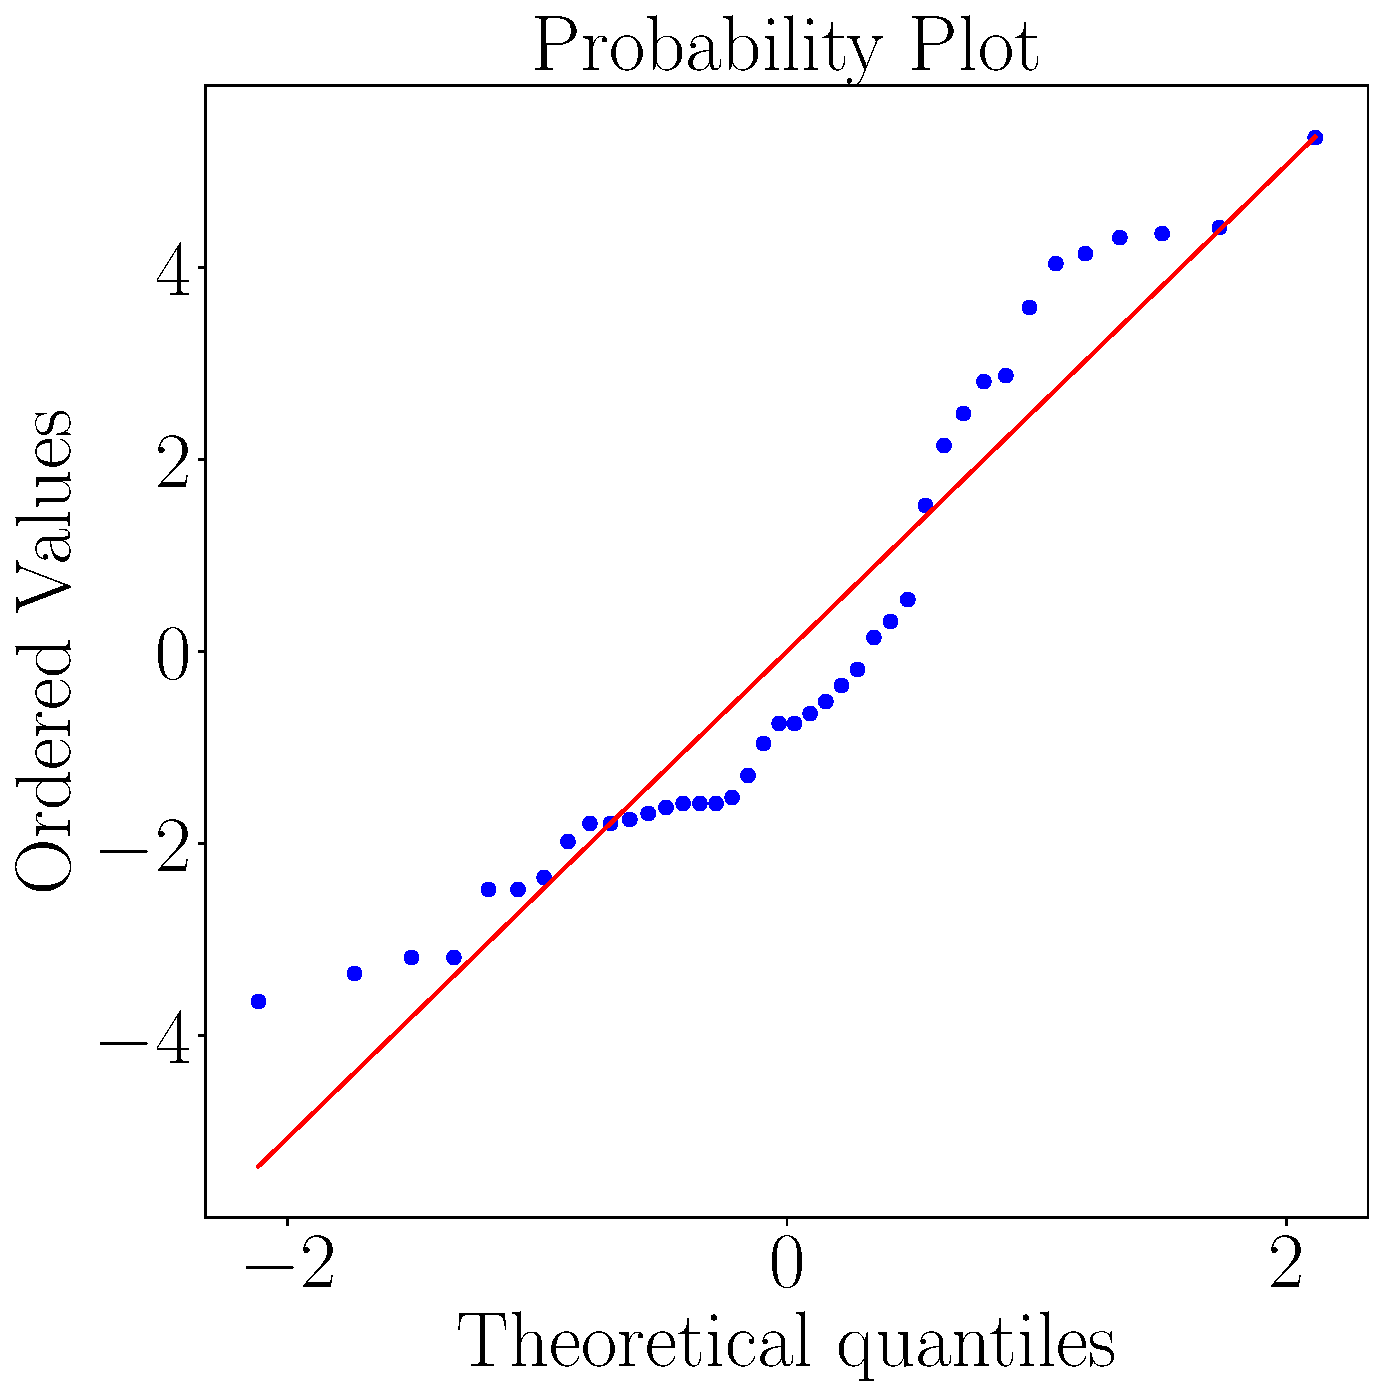
\includegraphics[width = \textwidth]{Resultados/Nasa/Figuras/pdf/qqplot_nasa_avg_two_way_blind.pdf}
        \caption{QQ plot of the NASA-TLX score of the blind participants on each method.}
        \label{fig:qqplot_nasa_avg_two_way_blind}
    \end{minipage}
    \begin{minipage}{0.075\textwidth}
        \hfill
    \end{minipage}
    \begin{minipage}{0.45\textwidth}
        %\vspace{2ex}
        \centering
        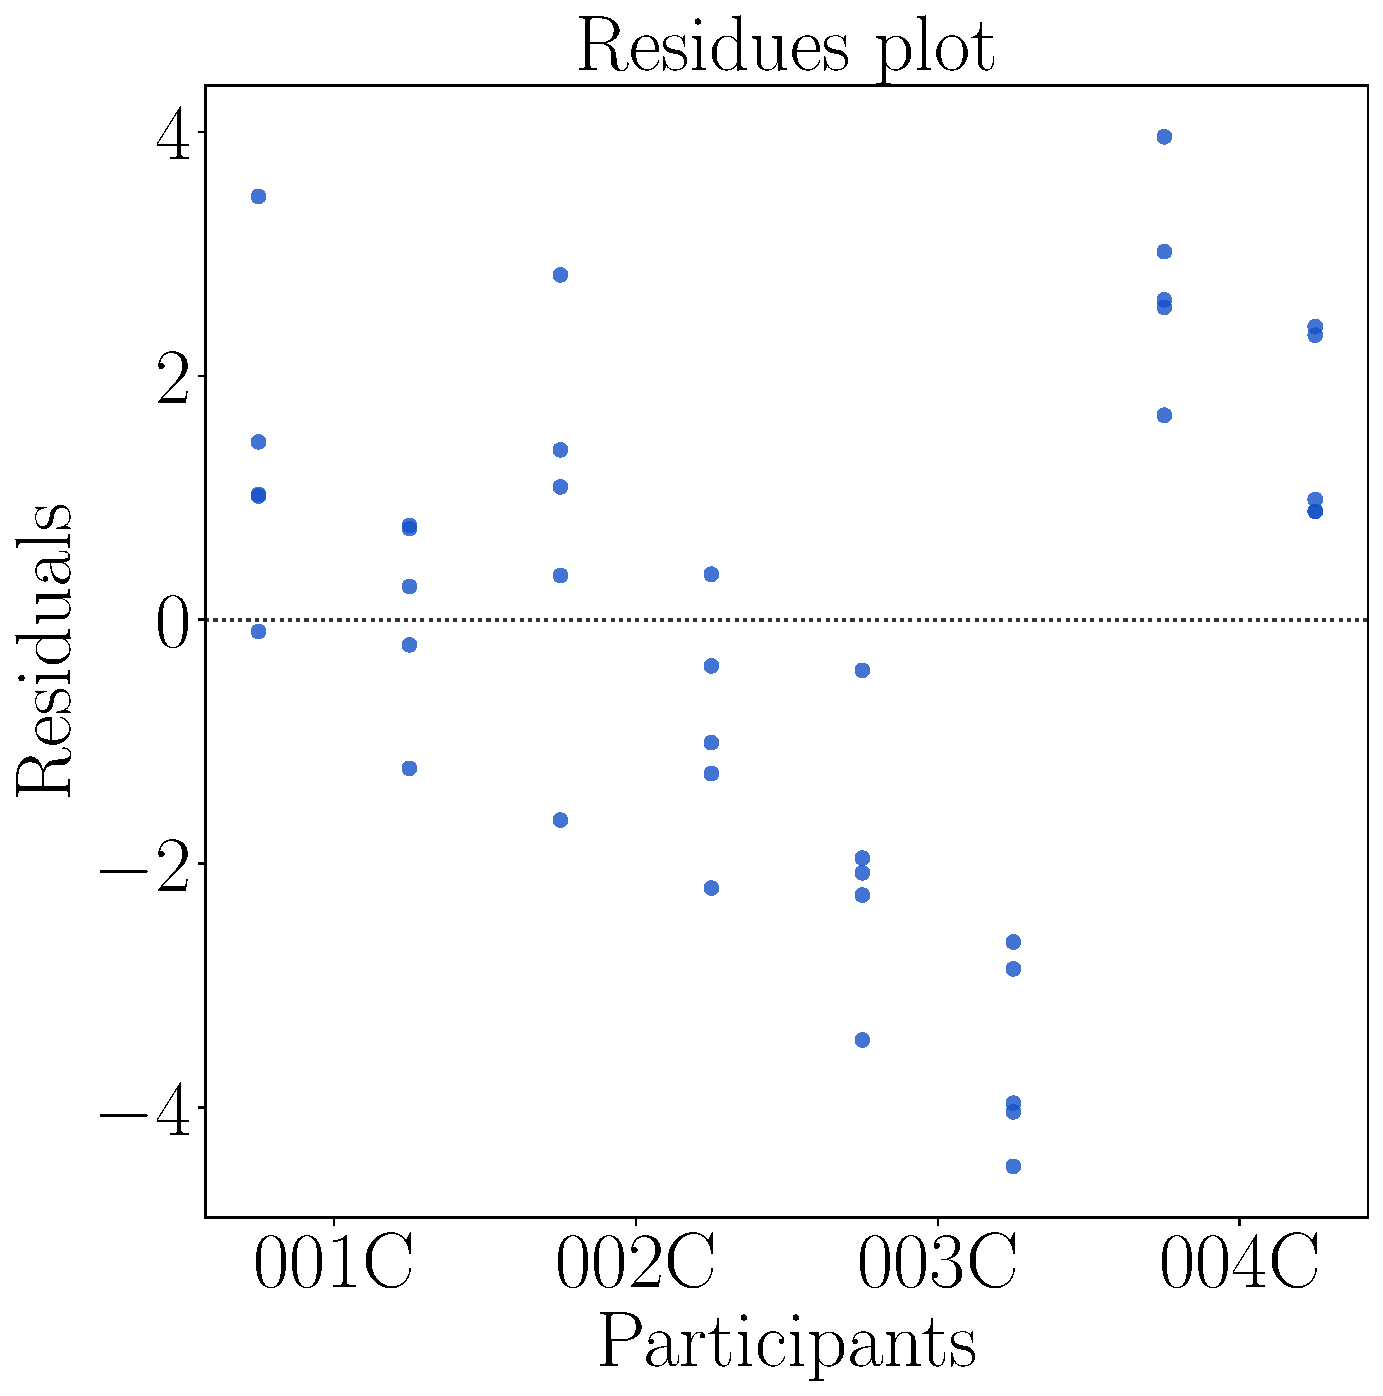
\includegraphics[width = \textwidth]{Resultados/Nasa/Figuras/pdf/residplot_nasa_avg_two_way_blind.pdf}
        \caption{Residual plot of the NASA-TLX score the blind participants on each method.}
        \label{fig:residplot_nasa_avg_two_way_blind}
    \end{minipage}
\end{figure}

Table \ref{tab:blocanova_nasa_avg_two_way_blind} brings the p-value resulting from ANOVA. In this case, both the methods and the rounds were appointed as significant variables that influence the mean value of the NASA-TLX global score. 


\begin{table}[!htb]
\centering
\caption{Anova p-value for the NASA-TLX score on each method for blinded users.}
\label{tab:blocanova_nasa_avg_two_way_blind}
\begin{tabular}{lrrrrl}
\toprule
          Source & P-Value \\
\midrule
    \    Methods & 0.029** \\
     \    Rounds & 0.022** \\
\    Interaction &   0.814 \\
\bottomrule
\end{tabular}
\end{table}



Finally, Table \ref{tab:lsd_nasa_avg_two_way_blind} presents the results of a pairwise Fisher LSD test comparing each pair of guidance methods. The results show that only "audio" is similar "base". All the other methods are different from each other.


\begin{table}[!htb]
\centering
\caption{Cross validation p-value for the NASA-TLX score on each method for blinded users.}
\label{tab:lsd_nasa_avg_two_way_blind}
\begin{tabular}{rclr}
\toprule
      \multicolumn{3}{c}{Method} &                                           Analysis \\
\midrule
              Base & $X$ & Audio &                   $H_0 : \mu_{Base} = \mu_{Audio}$ \\
        Base & $X$ & Haptic Belt &         $H_1 : \mu_{Base} \ne \mu_{Haptic Belt}**$ \\
       Base & $X$ & Virtual Cane &        $H_1 : \mu_{Base} \ne \mu_{Virtual Cane}**$ \\
            Base & $X$ & Mixture &             $H_1 : \mu_{Base} \ne \mu_{Mixture}**$ \\
       Audio & $X$ & Haptic Belt &        $H_1 : \mu_{Audio} \ne \mu_{Haptic Belt}**$ \\
      Audio & $X$ & Virtual Cane &       $H_1 : \mu_{Audio} \ne \mu_{Virtual Cane}**$ \\
           Audio & $X$ & Mixture &            $H_1 : \mu_{Audio} \ne \mu_{Mixture}**$ \\
Haptic Belt & $X$ & Virtual Cane & $H_1 : \mu_{Haptic Belt} \ne \mu_{Virtual Cane}**$ \\
     Haptic Belt & $X$ & Mixture &      $H_1 : \mu_{Haptic Belt} \ne \mu_{Mixture}**$ \\
    Virtual Cane & $X$ & Mixture &         $H_0 : \mu_{Virtual Cane} = \mu_{Mixture}$ \\
\bottomrule
\end{tabular}
\end{table}



Table \ref{tab:nasa_var_group_blind} shows the difference in the NASA-TLX global score between the first and return rounds. It shows that the "audio" difference is the lowest among all methods, while the highest difference is for the "virtual cane".


\begin{table}[!htb]
\centering
\caption{NASA-TLX score grouped by participant and visual Condition.}
\label{tab:nasa_var_group_blind}
\begin{tabular}{lrrrrrr}
\toprule
{} &   Base &  Audio & \begin{tabular}[c]{@{}l@{}}Haptic\\ Belt\end{tabular} & \begin{tabular}[c]{@{}l@{}}Virtual\\ Cane\end{tabular} & Mixture \\
Visual Condition &        &        &                                                       &                                                        &         \\
\midrule
Blind            &  -0.92 &  -0.25 &                                                 -1.21 &                                                  -1.54 &   -0.54 \\
\bottomrule
\end{tabular}
\end{table}



\FloatBarrier
\subsubsection{Adapted SAGAT}
\label{subsubsec:results_adapted_sagat_1}

In this subsection, the SAGAT questionnaire is analyzed. Its result may give an idea of the mental map the participant is drawing. For each question a participant could score 1 point or a fraction of it. The total score of each blind participant is presented on the Table \ref{tab:sagat_table_blind} and they are plotted in the Figures \ref{fig:barplot_sagat_avg_5_scene_blind}, where it is visually noticeable that the performance better the second time they visit the room. 


\begin{table}[!htb]
\centering
\caption{SAGAT global score felled by the blinded participants.}
\label{tab:sagat_table_blind}
\begin{tabular}{llrrrrr}
\toprule
     &        &   Base &  Audio & \begin{tabular}[c]{@{}l@{}}Haptic\\ Belt\end{tabular} & \begin{tabular}[c]{@{}l@{}}Virtual\\ Cane\end{tabular} & Mixture \\
Participant & Round &        &        &                                                       &                                                        &         \\
\midrule
001C & First &   6.25 &   5.50 &                                                  5.33 &                                                   5.83 &   3.500 \\
     & Return &   6.25 &   6.50 &                                                  8.50 &                                                   5.50 &   5.500 \\
002C & First &   6.75 &   4.50 &                                                  3.99 &                                                   4.50 &   6.250 \\
     & Return &   5.25 &   5.00 &                                                  4.00 &                                                   6.50 &   8.500 \\
003C & First &   7.25 &   7.50 &                                                  7.49 &                                                   4.66 &   9.000 \\
     & Return &  10.00 &  10.00 &                                                  8.50 &                                                   9.00 &   9.000 \\
004C & First &   7.50 &   6.00 &                                                  7.66 &                                                   4.99 &   6.500 \\
     & Return &   9.00 &   6.00 &                                                  9.25 &                                                   7.25 &   9.000 \\
\bottomrule
\end{tabular}
\end{table}



\begin{figure}[!htb]
    \centering
    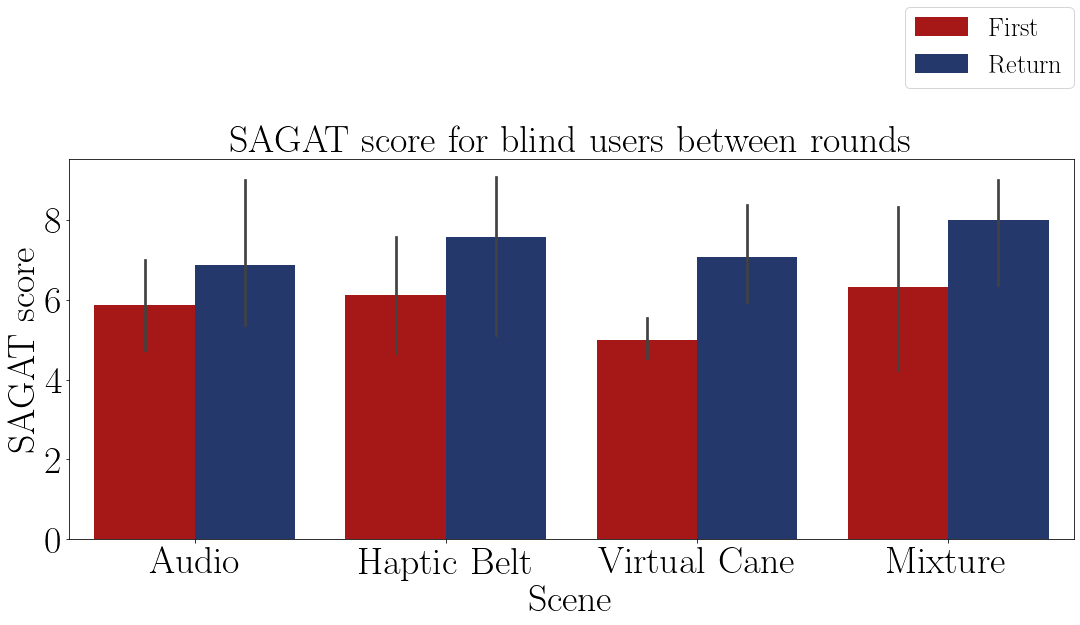
\includegraphics[width = 0.8\linewidth]{Resultados/Sagat/Figuras/png/barplot_sagat_avg_5_scene_blind.png}
    \caption{Barplot of the average SAGAT score of the blind participants on each method.}
    \label{fig:barplot_sagat_avg_5_scene_blind}
\end{figure}

The boxplot in the Figure \ref{fig:boxplot_sagat_blind_scene} shows that there are two groups of scores one with the “Base”, “Haptic Belt” and the “Mixture” methods, and the second group with the “Audio” and the “Virtual Cane” methods. The first group scored higher than the second one. The Figure \ref{fig:boxplot_sagat_blind_rounds} shows a noticible difference between the scores when grouped by their corresponding round.

\begin{figure}[!htb]
    \centering
    \begin{minipage}{0.45\textwidth}
        \centering
        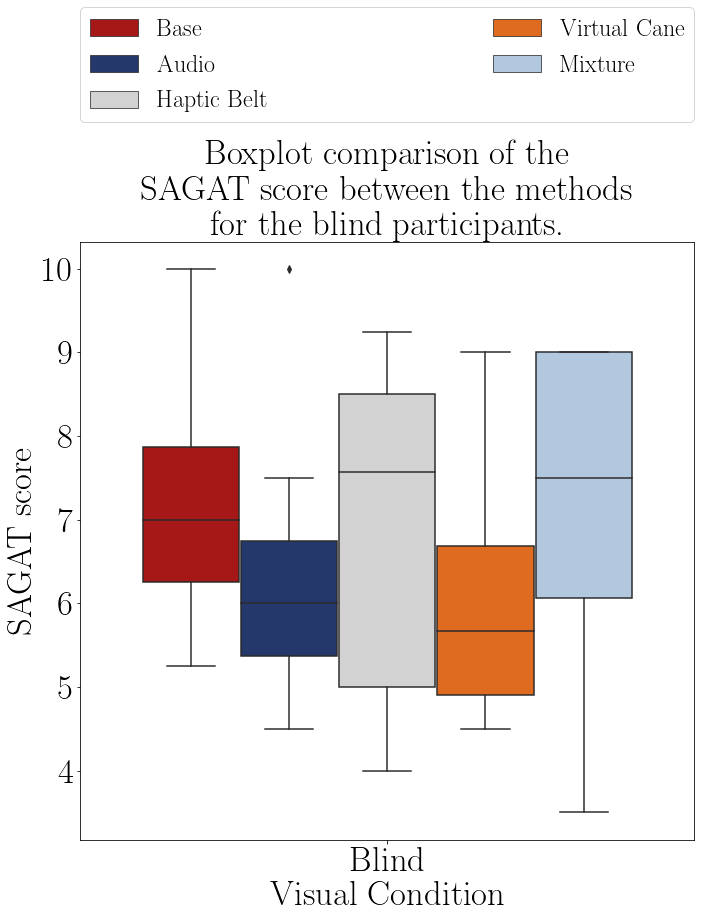
\includegraphics[width = 0.8\linewidth]{Resultados/Sagat/Figuras/png/boxplot_sagat_blind_scene.png}
        \caption{Boxplot of the SAGAT score of the blind participants grouped by method.}
        \label{fig:boxplot_sagat_blind_scene}
    \end{minipage}
    \begin{minipage}{0.45\textwidth}
        \centering
        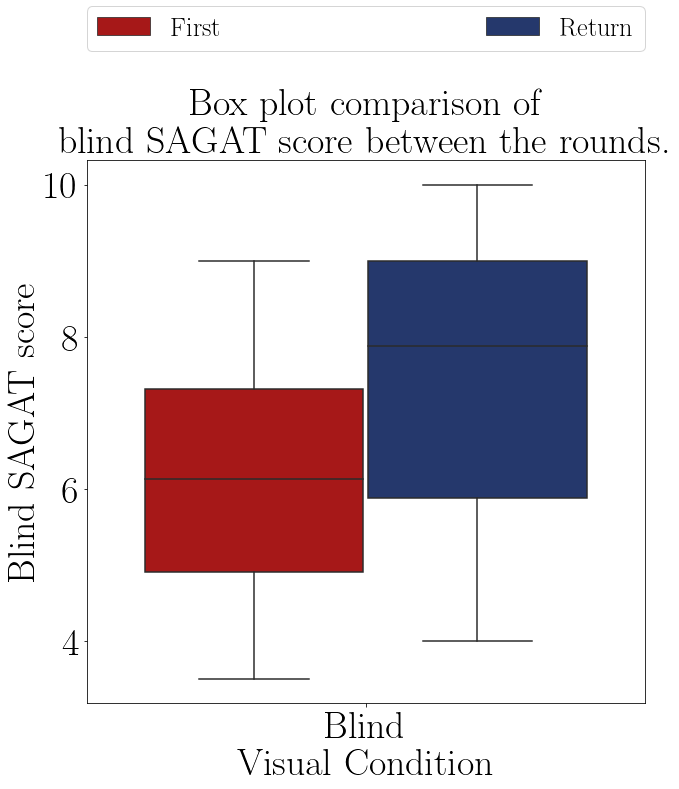
\includegraphics[width = 0.8\linewidth]{Resultados/Sagat/Figuras/png/boxplot_sagat_blind_rounds.png}
        \caption{Boxplot of the SAGAT score of the blind participants grouped by round.}
        \label{fig:boxplot_sagat_blind_rounds}
    \end{minipage}
\end{figure}

The Table \ref{tab:sagat_average_group_blind} shows the average SAGAT score in the “blind” sample and is possible to notice how the average score by the “blind” sample was lower during the “Audio” and the “Base” methods.


\begin{table}[!htb]
\centering
\caption{SAGAT score average grouped by participant and visual condition}
\label{tab:sagat_average_group_blind}
\begin{tabular}{lrrrrrr}
\toprule
{} &  Base & Audio & \begin{tabular}[c]{@{}l@{}}Haptic\\ Belt\end{tabular} & \begin{tabular}[c]{@{}l@{}}Virtual\\ Cane\end{tabular} &  Mixture \\
Visual Condition &       &       &                                                       &                                                        &          \\
\midrule
Blind            &  7.28 &  6.38 &                                                  6.84 &                                                   6.03 &    7.156 \\
\bottomrule
\end{tabular}
\end{table}




The Figures \ref{fig:qqplot_sagat_avg_two_way_blind} and \ref{fig:residplot_sagat_avg_two_way_blind} shows the distribution and variance of the Table \ref{tab:sagat_table_blind}. These Figures shows that the data are normally distributed and that the methods have a similar variance.
The Table \ref{tab:blocanova_sagat_avg_two_way_blind} shows the Anova test p-value of the SAGAT score of the "blind" sample. The round's p-values indicates that some have influence on the SAGAT score. Meaning that the participants did learn information about the room between the "First" and "Return" round. The method and the interaction between it and the round has no influence on the SAGAT score.


\begin{table}[!htb]
\centering
\caption{Anova p-value for the SAGAT score on each method for blinded users.}
\label{tab:blocanova_sagat_avg_two_way_blind}
\begin{tabular}{lrrrrr}
\toprule
               Source &  Squared sum &  DOF & Squared average &      F & \begin{tabular}[c]{@{}l@{}}P-Value \\ $(F_{0} > F)$\end{tabular} \\
\midrule
Participants (Blocks) &       48.231 &    3 &          16.077 &  9.731 &                                                                  \\
         \    Methods &        8.922 &    4 &           2.230 &  1.350 &                                                            0.277 \\
          \    Rounds &       18.975 &    1 &          18.975 & 11.485 &                                                          0.002** \\
     \    Interaction &        2.391 &    4 &           0.598 &  0.362 &                                                            0.834 \\
   Experimental Error &       44.608 &   27 &           1.652 &        &                                                                  \\
                Total &      123.127 &   39 &                 &        &                                                                  \\
\bottomrule
\end{tabular}
\end{table}



\begin{figure}[!htb]
    \centering
    \begin{minipage}{0.45\textwidth}
        \centering
        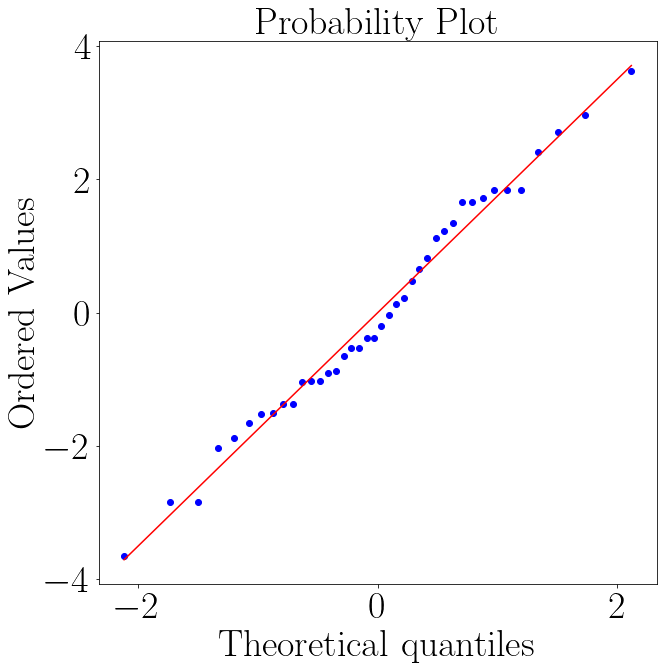
\includegraphics[width = 0.8\linewidth]{Resultados/Sagat/Figuras/png/qqplot_sagat_avg_two_way_blind.png}
        \caption{QQ plot of the SAGAT score of the blind participants on each method.}
        \label{fig:qqplot_sagat_avg_two_way_blind}
    \end{minipage}
    \begin{minipage}{0.45\textwidth}
        \centering
        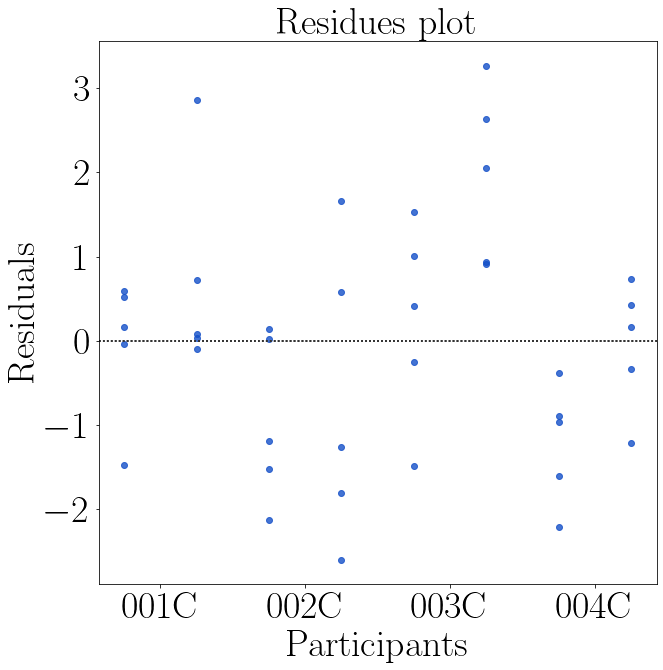
\includegraphics[width = 0.8\linewidth]{Resultados/Sagat/Figuras/png/residplot_sagat_avg_two_way_blind.png}
        \caption{Residual plot of the SAGAT score the blind participants on each method.}
        \label{fig:residplot_sagat_avg_two_way_blind}
    \end{minipage}
\end{figure}


%The Table \ref{tab:lsd_sagat_avg_two_way} presents the conclusion of a pairwise Fisher LSD test of the blind NASA-TLX score between all the guidance methods. The results show that only the "Audio" has a similar NASA-TLX score as the "Base" method, as it was also posible to notice at Figure \ref{fig:boxplot_sagat_blind_scene}.

%\input{Resultados/Sagat/Tabelas/lsd_sagat_avg_two_way}

The Table \ref{tab:sagat_var_group_blind} shows the average of the SAGAT score variation between the rounds. This table shows that the variation from the "Base" and the "Audio" was the lowest variation and the highest variation was the "Virtual Cane".


\begin{table}[!htb]
\centering
\caption{Adapted Sagat global score variation grouped by participant and visual Condition}
\label{tab:sagat_var_group_blind}
\begin{tabular}{lrrrrrr}
\toprule
{} &  Base &  Audio & \begin{tabular}[c]{@{}l@{}}Haptic\\ Belt\end{tabular} & \begin{tabular}[c]{@{}l@{}}Virtual\\ Cane\end{tabular} & Mixture \\
Visual Condition &       &        &                                                       &                                                        &         \\
\midrule
Blind            &  8.93 &  15.66 &                                                 23.49 &                                                  44.30 &   32.90 \\
\bottomrule
\end{tabular}
\end{table}



The Figures \ref{fig:qqplot_sagat_var_blind} and \ref{fig:residplot_sagat_var_blind} shows the distribution and variance of the SAGAT score variation of the Table \ref{tab:sagat_table_blind}. These Figures shows that the data are normally distributed and that the methods have a similar variance.
The Table \ref{tab:blocanova_sagat_var_blind} shows the Anova test p-value of the SAGAT score of the "blind" sample between the guidance methods. The p-value indicates that there are no difference between the variation in any method. 


\begin{table}[!htb]
\centering
\caption{Anova p-value for the SAGAT score variation on each method for blinded users.}
\label{tab:blocanova_sagat_var_blind}
\begin{tabular}{lrrrrr}
\toprule
               Source &  Squared sum &  DOF & Squared average &     F & \begin{tabular}[c]{@{}l@{}}P-Value \\ $(F_{0} > F)$\end{tabular} \\
\midrule
Participants (blocks) &     1176.902 &    3 &         782.885 & 0.473 &                                                                  \\
               Method &     3131.542 &    4 &         392.301 & 0.944 &                                                            0.472 \\
   Experimental error &     9956.458 &   12 &         829.705 &       &                                                                  \\
                Total &    14264.902 &   19 &                 &       &                                                                  \\
\bottomrule
\end{tabular}
\end{table}



\begin{figure}[!htb]
    \centering
    \begin{minipage}{0.45\textwidth}
        \centering
        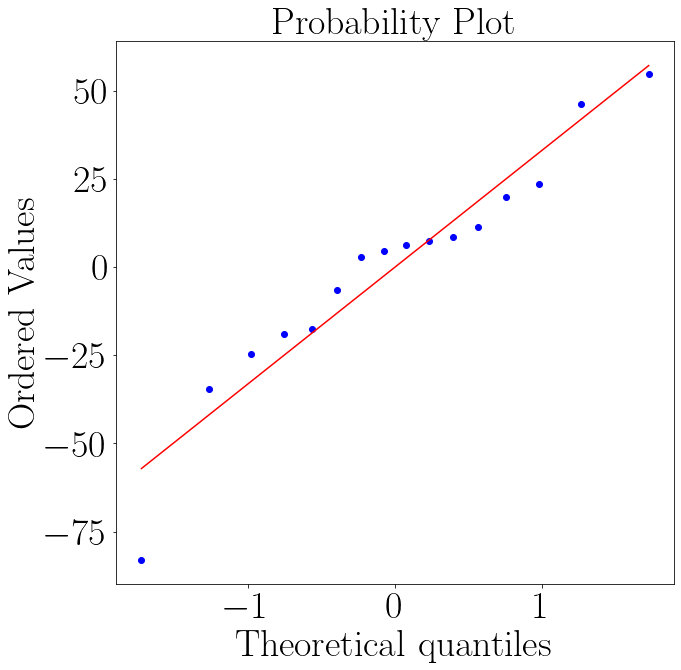
\includegraphics[width = 0.8\linewidth]{Resultados/Sagat/Figuras/png/qqplot_sagat_var_sight.png}
        \caption{QQ plot of the SAGAT score variation of the blind participants on each method.}
        \label{fig:qqplot_sagat_var_blind}
    \end{minipage}
    \begin{minipage}{0.45\textwidth}
        \centering
        \includegraphics[width = 0.8\linewidth]{Resultados/Sagat/Figuras/png/residplot_sagat_var_sight.png}
        \caption{Residual plot of the SAGAT score variation of the blind participants on each method.}
        \label{fig:residplot_sagat_var_blind}
    \end{minipage}
\end{figure}

%The Table \ref{tab:lsdbloc_nasa_var} presents the conclusion of a pairwise Fisher LSD test of the blind NASA-TLX score between all the guidance methods. The results show that all methods have similar variations.

%
\begin{table}[!htb]
\centering
\caption{Cross validation p-value for the NASA-TLX score variation on each method for blinded users.}
\label{tab:lsdbloc_nasa_var}
\begin{tabular}{rclr}
\toprule
      \multicolumn{3}{c}{Method} &                                       Analysis \\
\midrule
              Base & $X$ & Audio &           $H_1 : \mu_{Base} \ne \mu_{Audio}**$ \\
        Base & $X$ & Haptic Belt &         $H_0 : \mu_{Base} = \mu_{Haptic Belt}$ \\
       Base & $X$ & Virtual Cane &    $H_1 : \mu_{Base} \ne \mu_{Virtual Cane}**$ \\
            Base & $X$ & Mixture &             $H_0 : \mu_{Base} = \mu_{Mixture}$ \\
       Audio & $X$ & Haptic Belt &    $H_1 : \mu_{Audio} \ne \mu_{Haptic Belt}**$ \\
      Audio & $X$ & Virtual Cane &   $H_1 : \mu_{Audio} \ne \mu_{Virtual Cane}**$ \\
           Audio & $X$ & Mixture &            $H_0 : \mu_{Audio} = \mu_{Mixture}$ \\
Haptic Belt & $X$ & Virtual Cane & $H_0 : \mu_{Haptic Belt} = \mu_{Virtual Cane}$ \\
     Haptic Belt & $X$ & Mixture &  $H_1 : \mu_{Haptic Belt} \ne \mu_{Mixture}**$ \\
    Virtual Cane & $X$ & Mixture & $H_1 : \mu_{Virtual Cane} \ne \mu_{Mixture}**$ \\
\bottomrule
\end{tabular}
\end{table}



To close up, according to the ANOVA test at Table \ref{tab:blocanova_sagat_avg_two_way_blind} the methods caused no reaction on the SAGAT score, but the rounds did. That means that the participants were able in all methods to learn a little about their environment and that learning impacted their environmental perception in the next round. The fact that the test has not found any influence of the methods on the SAGAT score may be because of the small sample size, since it is posible to notice a difference between the methods at Figure \ref{fig:boxplot_sagat_blind_scene}. Also the interaction between method and round caused no influence in the Sagat score. According to the ANOVA test at Table \ref{tab:blocanova_sagat_var_blind}, the methods did not influenced the SAGAT score.

\FloatBarrier
\subsubsection{Guidance method's questionnaire.}
\label{subsubsec:results_questionnaires}

Finally, the data from the questionnaire for evaluating the user experience with each guidance method is also analysed. The higher the score, the more satisfied the user is with the method. It is important to observe that this analysis does not include the ‘base’ method as the questions are specific about each method and the ‘base’ may vary among the participants. Also, there is no distinction between first and return rounds. Each questionnaire is answered only once for each method

Table \ref{tab:questionnaire_average_blind} presents the score attributed to each method by each participant. The mean values are plotted in the Figure \ref{fig:barplot_questionnaire_scene_blind} and show a dissatisfaction with the methods that only use vibration for communicating with the participant, i.e., the haptic belt and the virtual cane. 


\begin{table}[!htb]
\centering
\caption{ Guidance method questionnaire score felled by the blinded participants.}
\label{tab:questionnaire_average_blind}
\begin{tabular}{llrrrrr}
\toprule
{} &  Audio &  \begin{tabular}[c]{@{}l@{}}Haptic\\ Belt\end{tabular} &  \begin{tabular}[c]{@{}l@{}}Virtual\\ Cane\end{tabular} &  Mixture \\
Participant &        &                                                        &                                                         &          \\
\midrule
001C        &  0.774 &                                                  0.543 &                                                   0.629 &    0.865 \\
002C        &  0.857 &                                                  0.743 &                                                   0.543 &    0.935 \\
003C        &  0.929 &                                                  0.571 &                                                   0.543 &    0.745 \\
004C        &  0.881 &                                                  0.486 &                                                   0.400 &    0.730 \\
\bottomrule
\end{tabular}
\end{table}



\begin{figure}[!htb]
    \centering
    \includegraphics[width = 0.8\linewidth]{Resultados/Questionario/Figuras/png/barplot_questionnaire_scene_blind.png}
    \caption{Barplot of the average questionaire score of the blind participants on each method.}
    \label{fig:barplot_questionnaire_scene_blind}
\end{figure}

Figure \ref{fig:boxplot_quest_blind_scene} brings the questionnaire boxplot, which clearly shows the difference between two groups: haptic belt and virtual cane, and audio and mixture. 

\begin{figure}[!htb]
    \centering
    \includegraphics[width = 0.6\linewidth]{Resultados/Questionario/Figuras/png/boxplot_questionnaire_scene_blind.png}
    \caption{Boxplot of the questionaire score of the blind participants grouped by method.}
    \label{fig:boxplot_quest_blind_scene}
\end{figure}

%The Table \ref{tab:questionnaire_average_group_blind} show the the average questionnaire score on each method. It also shows a disatisfaction with the haptic devices alone.
%
%
\begin{table}[!htb]
\centering
\caption{Guidance method questionnaire average score for the blind participants.}
\label{tab:questionnaire_average_group_blind}
\begin{tabular}{lrrrrr}
\toprule
{} & Audio & Haptic Belt & Virtual Cane & Mixture \\
Visual Condition &       &             &              &         \\
\midrule
Blind            &  0.86 &        0.59 &         0.53 &    0.82 \\
\bottomrule
\end{tabular}
\end{table}



Following, Figures \ref{fig:qqplot_questionnaires} and \ref{fig:residplot_questionnaires} shows that the data follows a normal distribution. However, the residual variance is not exactly homogenous among the participants. 

\begin{figure}[!htb]
    \centering
    \begin{minipage}{0.45\textwidth}
        \centering
        \includegraphics[width = 0.8\linewidth]{Resultados/Questionario/Figuras/png/qqplot_questionnaires.png}
        \caption{QQ plot of the questionnaire score of the blind participants on each method.}
        \label{fig:qqplot_questionnaires}
    \end{minipage}
    \begin{minipage}{0.45\textwidth}
        \centering
        \includegraphics[width = 0.8\linewidth]{Resultados/Questionario/Figuras/png/residplot_questionnaires.png}
        \caption{Residual plot of the questionnaire score the blind participants on each method.}
        \label{fig:residplot_questionnaires}
    \end{minipage}
\end{figure}

The results of ANOVA are presented in Table  \ref{tab:blocanova_questionnaire} and shows that the method, with a p-value of 0.001, is indeed a significant variable that affects the user satisfaction.


\begin{table}[!htb]
\centering
\caption{Anova p-value for the questionnaire score on each method for blinded users.}
\label{tab:blocanova_questionnaire}
\begin{tabular}{lrrrrr}
\toprule
               Source &  Squared sum &  DOF & Squared average &      F & \begin{tabular}[c]{@{}l@{}}P-Value \\ $(F_{0} > F)$\end{tabular} \\
\midrule
Participants (blocks) &        0.042 &    3 &           0.110 &  2.014 &                                                                  \\
               Method &        0.329 &    3 &           0.014 & 15.677 &                                                          0.001** \\
   Experimental error &        0.063 &    9 &           0.007 &        &                                                                  \\
                Total &        0.434 &   15 &                 &        &                                                                  \\
\bottomrule
\end{tabular}
\end{table}



In order to complement the ANOVA analysis, the pairwise comparison of the methods, obtained from the Fisher LSD test, is presented in Table \ref{tab:lsd_questionnaire}. The results show that ‘audio’ and ‘mixture’ are equivalent from the perspective of user satisfaction. All the other comparisons indicate there is a difference between the methods.


\begin{table}[!htb]
\centering
\caption{Cross validation p-value for the questionnaire score on each method for blinded users.}
\label{tab:lsd_questionnaire}
\begin{tabular}{rclr}
\toprule
      \multicolumn{3}{c}{Method} &                                           Analysis \\
\midrule
       Audio & $X$ & Haptic Belt &        $H_1 : \mu_{Audio} \ne \mu_{Haptic Belt}**$ \\
      Audio & $X$ & Virtual Cane &       $H_1 : \mu_{Audio} \ne \mu_{Virtual Cane}**$ \\
           Audio & $X$ & Mixture &                $H_0 : \mu_{Audio} = \mu_{Mixture}$ \\
Haptic Belt & $X$ & Virtual Cane & $H_1 : \mu_{Haptic Belt} \ne \mu_{Virtual Cane}**$ \\
     Haptic Belt & $X$ & Mixture &          $H_0 : \mu_{Haptic Belt} = \mu_{Mixture}$ \\
    Virtual Cane & $X$ & Mixture &     $H_1 : \mu_{Virtual Cane} \ne \mu_{Mixture}**$ \\
\bottomrule
\end{tabular}
\end{table}



Additional to the scores, the participants also expressed their dissatisfaction in the answers to the open questions of the questionnaire, where they commented that the haptic belt and the virtual cane are confusing, are not enough precise, and are very different from what they are used to.

\FloatBarrier

\subsection{Physiological data}

During the experiment, data from two physiological sensors were captured: ECG and GSR. As commonly found in the literature, these data are used to assess mental workload. The corresponding analysis is presented in this section.

\subsubsection{Electrocardiogram (ECG) data}
\label{subsubsec:results_ecg_1}

As previously stated, the ECG analysis is based on two variables: the heartrate (BPM – beats per minute) and heartrate variance (SDNN – standard deviation of NN intervals). 

After the experiment, the ECG signal processing is organized in the following steps (Figure \ref{fig:ecg_algorithim}): 

\begin{itemize}
    \item Filtering and removing outliers. Since the participants moved during the whole experience, the sensors also captured some noise data.
    \item Normalization between -1 and 1;
    \item Peak detection and evaluation – if the results were not of good quality, the peak detection method's parameters were adjusted to improve it; 
    \item Calculation of BPM using Kubius HRV Standard;
    \item Calculation of SDNN using Kubius HRV Standard.
\end{itemize}

\begin{figure}[H]
    \centering
    \tikzstyle{start} = [rectangle, rounded corners, minimum width=4cm, minimum height=1.0cm,text centered, draw=black, fill=white!30, text width=3cm]
\tikzstyle{process} = [rectangle, minimum width=4cm, minimum height=1.0cm, text centered, draw=black, fill=white!30, text width=3.5cm]
\tikzstyle{decision} = [diamond, minimum width=3.5cm, minimum height=1.0cm,  text centered, text width=3.5cm, draw=black, fill=white!30]
\tikzstyle{arrow_flow} = [ccmDBlue, rounded corners, line width = 2mm, ->]
\tikzstyle{arrow_return} = [ccmRed, rounded corners, line width = 2mm, ->]

\begin{tikzpicture}[node distance=2cm]
    \centering
    \node (start) [start] {Collect the ECG Data};
    \node (read) [process, below of=start,yshift=-0.5cm] {Python - Read the ECG file};
    \node (outlier) [process, aspect=2.5, below of=read, yshift=-0.5cm, text width=4cm] {Python - Remove the outlier noise};
    \node (normalize) [process, aspect=2.5, below of=outlier, yshift=-0.5cm] {Python - Normalize (-1 and 1)};
    \node (findPeaks) [process, aspect=2.5, below of=normalize, yshift=-0.5cm] {Python - Run peak finder};
    \node (graphical) [decision, aspect=2.5, below of=findPeaks, yshift=-1cm] {Graphical analysis};

    \node (no_graphical) [process, below of=graphical, yshift=-0.75cm] {Python - Tune the peak finder};

    \node (yes_graphical) [process, right of=graphical, xshift=2.5cm, yshift=2.5cm]{Python - Calculate the time difference between peaks};
    \node (savePeak) [process, above of=yes_graphical, yshift=1.0cm, text width=4cm]{Python - Save the peak file};
    \node (readPeak) [process, above of=savePeak, yshift=0.5cm, text width=4cm] {Kubius - Read the peak file};
    \node (analysis) [process, above of=readPeak, yshift=0.5cm, text width=4cm] {Kubius - Run Analysis};
    \node (saveAnalysis) [process, right of=analysis, xshift=2.5cm, yshift=-2.5cm] {Kubius - Save a report file};
    \node (readAnalysis) [process, below of=saveAnalysis, yshift=-1.0cm] {Python - Read report file};
    
    \draw [arrow_flow] (start.south) -- (read.north);
    \draw [arrow_flow] (read.south) -- (outlier.north);
    \draw [arrow_flow] (outlier.south) -- (normalize.north);
    \draw [arrow_flow] (normalize.south) -- (findPeaks.north);
    \draw [arrow_flow] (findPeaks.south) -- (graphical.north);
    
    \draw [arrow_flow] (graphical.east) -- node[anchor=north] {Peaks fit} +(1.8,0) -- (yes_graphical.south);
    \draw [arrow_flow] (yes_graphical.north) -- (savePeak.south);
    \draw [arrow_flow] (savePeak.north) -- (readPeak.south);
    \draw [arrow_flow] (readPeak.north) -- (analysis.south);
    \draw [arrow_flow] (analysis.east) -- ++(2.4,0) -- (saveAnalysis.north);
    \draw [arrow_flow] (saveAnalysis.south) -- (readAnalysis.north);
    \draw [arrow_return] (readAnalysis) -- ++(0,-1.5) -- ++(2.25,0) -- (11.25,1) -- (-3,1) -- (-3,-2.5) -- (read.west);
    
    \draw [arrow_flow] (graphical.west) -- ++(-0.3,0) -- node[anchor=south west] {Peaks} node[anchor=west] {fit not} ++(0,-2.75) -- (no_graphical.west);

    \draw [arrow_return] (no_graphical.north) -- (graphical.south);
    
\end{tikzpicture}
    \caption{ECG's data treatment algorithim.}
    \label{fig:ecg_algorithim}
\end{figure}

At the beginning of each experiment, a baseline was collected to establish a comparison between the relaxed state of the participant and the scenes' induced state. However, the results were not consistent.  During the experiment, it was expected that the heartrate would increase compared to the baseline because the participants were at rest. However, for most of the participants, it decreased, indicating a systematic problem may have occurred. Due to this fact, the analysis is based only on absolute values.

\paragraph{Analysis of the heartbeat frequency (BPM)}\mbox{}\\

Table \ref{tab:bpm_table_blind} presents the heart rate of each blind participant for each guidance method. If the variation between the First and the Return round is positive, it means that the user had an increase on his/her mental workload and vice-versa. It is possible to observe that there is no systematic difference between the methods. Also, there are significant differences among the participants, with some presenting values significantly lower than others.


\begin{table}[!htb]
\centering
\caption{Average BPM felled by the blinded participants [BPM].}
\label{tab:bpm_table_blind}
\begin{tabular}{llrrrrr}
\toprule
     &        &   Base &  Audio & \begin{tabular}[c]{@{}l@{}}Haptic\\ Belt\end{tabular} & \begin{tabular}[c]{@{}l@{}}Virtual\\ Cane\end{tabular} & Mixture \\
Participant & Round &        &        &                                                       &                                                        &         \\
\midrule
001C & First &  75.75 &  60.71 &                                                 71.17 &                                                  59.07 &   68.24 \\
     & Return &  71.05 &  58.61 &                                                 66.22 &                                                  64.20 &   70.76 \\
002C & First &  48.69 &  38.67 &                                                 48.74 &                                                  46.89 &   52.23 \\
     & Return &  52.46 &  47.58 &                                                 58.97 &                                                  56.75 &   58.25 \\
003C & First &  68.37 &  69.89 &                                                 70.95 &                                                  69.41 &   66.94 \\
     & Return &  67.34 &  67.44 &                                                 69.68 &                                                  68.82 &   67.37 \\
004C & First &  75.09 &  73.55 &                                                 73.70 &                                                  71.94 &   74.03 \\
     & Return &  74.74 &  74.79 &                                                 74.02 &                                                  72.69 &   67.34 \\
\bottomrule
\end{tabular}
\end{table}



Figure \ref{fig:barplot_ecg_bpm_5_scene_blind} presents the mean heart rate. It shows a slight increase in the heartrate between the rounds, except for the base method, indicating that the participants had a higher Mental Workload on the return round.

\begin{figure}[!htb]
    \centering
    \includegraphics[width = \textwidth]{Resultados/ECG/Figuras/pdf/barplot_ecg_bpm_5_scene_blind.pdf}
    \caption{Barplot of the average BPM of the blind participants on each method.}
    \label{fig:barplot_ecg_bpm_5_scene_blind}
\end{figure}

%The Table \ref{tab:bpm_average_group_blind} show the average heartbeat frequency variation between the rounds of each group. As it was shown in the Figure \ref{fig:barplot_ecg_bpm_5_scene_blind}, only the Base method has a negative average variaton between the rounds. It is also posible to see that the Virtual Cane variation was the highest, hence it was also the highest mental workload.
% 
%
\begin{table}[!htb]
\centering
\caption{ECG average BPM  for each method of the blind participants.}
\label{tab:bpm_average_group_blind}
\begin{tabular}{lrrrrr}
\toprule
{} &   Base & Audio & Haptic Belt & Virtual Cane & Mixture \\
Visual Condition &        &       &             &              &         \\
\midrule
Blind            &  -0.58 &  1.40 &        1.09 &         3.79 &    0.57 \\
\bottomrule
\end{tabular}
\end{table}



Figures \ref{fig:boxplot_ecg_bpm_blind_scene} and \ref{fig:boxplot_ecg_bpm_blind_rounds} brings the corresponding boxplot, grouped by method and round. In both cases, it is not possible to observe significant differences among the methods or rounds.

\begin{figure}[!htb]
    \centering
    \begin{minipage}{0.45\textwidth}
        \centering
        \includegraphics[width = \textwidth]{Resultados/ECG/Figuras/pdf/boxplot_ecg_bpm_blind_scene.pdf}
        \caption{Boxplot of the BPM of the blind participants grouped by the methods.}
        \label{fig:boxplot_ecg_bpm_blind_scene}
    \end{minipage}
    \begin{minipage}{0.075\textwidth}
        \hfill
    \end{minipage}
    \begin{minipage}{0.45\textwidth}
        \centering
        \includegraphics[width = \textwidth]{Resultados/ECG/Figuras/pdf/boxplot_ecg_bpm_blind_rounds.pdf}
        \caption{Boxplot of the BPM of the blind participants grouped by the rounds.}
        \label{fig:boxplot_ecg_bpm_blind_rounds}
    \end{minipage}
\end{figure}

Figures \ref{fig:qqplot_bpm_two_way_blind} and \ref{fig:residplot_bpm_two_way_blind} bring the QQ Plot and residual distribution. The last one shows that the participants do not have a similar variance, which may jeopardize the results of ANOVA. Considering this limitation, Table \ref{tab:bpm_table_blind} brings the p-value obtained by ANOVA, which confirmed the previous analysis, as it does not indicate a significant influence of either the guidance methods or the rounds in the participants' heartrate. 

\begin{figure}[!htb]
    \centering
    \begin{minipage}{0.45\textwidth}
        \centering
        \includegraphics[width = \textwidth]{Resultados/ECG/Figuras/pdf/qqplot_bpm_two_way_blind.pdf}
        \caption{QQ plot of the BPM of the blind participants on each method.}
        \label{fig:qqplot_bpm_two_way_blind}
    \end{minipage}
    \begin{minipage}{0.075\textwidth}
        \hfill
    \end{minipage}
    \begin{minipage}{0.45\textwidth}
        \centering
        \includegraphics[width = \textwidth]{Resultados/ECG/Figuras/pdf/residplot_bpm_two_way_blind.pdf}
        \caption{Residual plot of the BPM score the blind participants on each method.}
        \label{fig:residplot_bpm_two_way_blind}
    \end{minipage}
\end{figure}


\begin{table}[!htb]
\centering
\caption{Anova p-value for the BPM on each method for blinded users.}
\label{tab:blocanova_bpm_two_way_blind}
\begin{tabular}{lrrrrr}
\toprule
               Source &  Squared sum &  DOF & Squared average &      F & \begin{tabular}[c]{@{}l@{}}P-Value \\ $(F_{0} > F)$\end{tabular} \\
\midrule
Participants (Blocks) &     2807.274 &    3 &         935.758 & 49.361 &                                                                  \\
         \    Methods &      164.045 &    4 &          41.011 &  2.163 &                                                            0.100 \\
          \    Rounds &       15.693 &    1 &          15.693 &  0.828 &                                                            0.371 \\
     \    Interaction &       20.606 &    4 &           5.152 &  0.272 &                                                            0.894 \\
   Experimental Error &      511.853 &   27 &          18.958 &        &                                                                  \\
                Total &     3519.471 &   39 &                 &        &                                                                  \\
\bottomrule
\end{tabular}
\end{table}



%
\begin{table}[!htb]
\centering
\caption{Cross validation p-value for the average BPM on each method for blinded users.}
\label{tab:lsd_bpm_two_way}
\begin{tabular}{rclr}
\toprule
      \multicolumn{3}{c}{Method} &                                           Analysis \\
\midrule
              Base & $X$ & Audio &               $H_1 : \mu_{Base} \ne \mu_{Audio}**$ \\
        Base & $X$ & Haptic Belt &             $H_0 : \mu_{Base} = \mu_{Haptic Belt}$ \\
       Base & $X$ & Virtual Cane &        $H_1 : \mu_{Base} \ne \mu_{Virtual Cane}**$ \\
            Base & $X$ & Mixture &             $H_1 : \mu_{Base} \ne \mu_{Mixture}**$ \\
       Audio & $X$ & Haptic Belt &        $H_1 : \mu_{Audio} \ne \mu_{Haptic Belt}**$ \\
      Audio & $X$ & Virtual Cane &       $H_1 : \mu_{Audio} \ne \mu_{Virtual Cane}**$ \\
           Audio & $X$ & Mixture &            $H_1 : \mu_{Audio} \ne \mu_{Mixture}**$ \\
Haptic Belt & $X$ & Virtual Cane & $H_1 : \mu_{Haptic Belt} \ne \mu_{Virtual Cane}**$ \\
     Haptic Belt & $X$ & Mixture &      $H_1 : \mu_{Haptic Belt} \ne \mu_{Mixture}**$ \\
    Virtual Cane & $X$ & Mixture &     $H_1 : \mu_{Virtual Cane} \ne \mu_{Mixture}**$ \\
\bottomrule
\end{tabular}
\end{table}



%The Table \ref{tab:lsd_bpm_two_way} presents the conclusion of a pairwise Fisher LSD test of the blind heart rate frequency variation between all the guidance methods. The results show that the only the Base and haptic belt have simila reaction.

%\FloatBarrier

%%%%%%%%%%%%%%%%%%%%%%%%%%%%%%%%%%%%%%%%%%%%%%%%%%%%%%%%%%%%%%%%%%%%%%%%%%%%
%%%%%%%%%%%%%%%%%%%%%%%%%%%%%%%%%%%%%%%%%%%%%%%%%%%%%%%%%%%%%%%%%%%%%%%%%%%%
%%%%%%%%%%%%%%%%%%%%%%%%%%%%%%%%%%%%%%%%%%%%%%%%%%%%%%%%%%%%%%%%%%%%%%%%%%%%
%%%%%%%%%%%%%%%%%%%%%%%%%%%%%%%%%%%%%%%%%%%%%%%%%%%%%%%%%%%%%%%%%%%%%%%%%%%%
%
%
\paragraph{Analysis of the heartbeat variance (SDNN)}\mbox{}\\
%
Table \ref{tab:sdnn_table_blind} brings the value of the second variable extracted from the ECG: SDNN, the standard deviation of the interbeat interval. Different to the heartrate frequency, if the variation between the First and the Return round is negative, it means that the user had an increase on his/her mental workload and vice-versa. Similar to what is observed for the BPM, it is not possible to draw a pattern from this data. The participants had increased or decreased their heartrate with different methods.


\begin{table}[!htb]
\centering
\caption{Average SDNN of the blind participants during the each round and method [ms].}
\label{tab:sdnn_table_blind}
\begin{tabular}{llrrrrr}
\toprule
     &        &    Base &   Audio &  \begin{tabular}[c]{@{}l@{}}Haptic\\ Belt\end{tabular} &  \begin{tabular}[c]{@{}l@{}}Virtual\\ Cane\end{tabular} &  Mixture \\
Participant & Round &         &         &                                                        &                                                         &          \\
\midrule
001C & First &  81.292 & 107.061 &                                                124.737 &                                                 163.968 &  129.054 \\
     & Return & 120.719 & 130.885 &                                                131.590 &                                                 157.589 &  124.786 \\
002C & First &  73.761 &  98.863 &                                                 81.140 &                                                  33.977 &   79.289 \\
     & Return & 108.940 &  49.627 &                                                 42.815 &                                                 114.057 &  107.545 \\
003C & First &  36.870 &  38.325 &                                                 35.101 &                                                  42.392 &   43.692 \\
     & Return &  52.750 &  41.196 &                                                 44.256 &                                                  42.602 &   46.145 \\
004C & First &  70.728 &  86.827 &                                                 62.560 &                                                  85.900 &   70.472 \\
     & Return &  71.950 &  74.895 &                                                 70.017 &                                                  66.089 &  104.040 \\
\bottomrule
\end{tabular}
\end{table}



The barplot of Figure \ref{fig:barplot_ecg_sdnn_5_scene_blind} shows the average SDNN for each method. It is possible to notice that some methods are associated with an increase in the SDNN between the rounds, while others present a slight decrease.

\begin{figure}[!htb]
    \centering
    \includegraphics[width = \textwidth]{Resultados/ECG/Figuras/pdf/barplot_ecg_sdnn_5_scene_blind.pdf}
    \caption{Barplot of the average SDNN of the blind participants on each method.}
    \label{fig:barplot_ecg_sdnn_5_scene_blind}
\end{figure}

%The Table \ref{tab:sdnn_average_group_blind} presents the average SDNN variation between the rounds. It shows that only the audio and the haptic belt methods shown a increase in the mental workload.
%
%
\begin{table}[!htb]
\centering
\caption{ECG average SDNN for each method of the blind participants.}
\label{tab:sdnn_average_group_blind}
\begin{tabular}{lrrrrr}
\toprule
{} &   Base &  Audio & Haptic Belt & Virtual Cane & Mixture \\
Visual Condition &        &        &             &              &         \\
\midrule
Blind            &  77.13 &  78.46 &       74.03 &        88.32 &   88.13 \\
\bottomrule
\end{tabular}
\end{table}



Figure \ref{fig:boxplot_ecg_sdnn_blind_scene} and Figure \ref{fig:boxplot_ecg_sdnn_blind_rounds} bring the SDNN barplot grouped by the methods and the rounds. There is a slight tendency among the participants to increase the heartbeat in the return round.

\begin{figure}[!htb]
    \centering
    \begin{minipage}{0.45\textwidth}
        \centering
        \includegraphics[width = \textwidth]{Resultados/ECG/Figuras/pdf/boxplot_ecg_sdnn_blind_scene.pdf}
        \caption{Boxplot of the SDNN of the blind participants grouped by the methods.}
        \label{fig:boxplot_ecg_sdnn_blind_scene}
    \end{minipage}
    \begin{minipage}{0.075\textwidth}
        \hfill
    \end{minipage}
    \begin{minipage}{0.45\textwidth}
        \centering
        \includegraphics[width = \textwidth]{Resultados/ECG/Figuras/pdf/boxplot_ecg_sdnn_blind_rounds.pdf}
        \caption{Boxplot of the SDNN of the blind participants grouped by the rounds.}
        \label{fig:boxplot_ecg_sdnn_blind_rounds}
    \end{minipage}
\end{figure}


Figures \ref{fig:qqplot_sdnn_two_way_blind} and \ref{fig:residplot_sdnn_two_way_blind} bring the QQ Plot and residual distribution. In this case, the residual distribution is more uniform than in Figure \ref{fig:residplot_bpm_two_way_blind}. The ANOVA results are presented in Table \ref{tab:blocdanova_sdnn_two_way_blind} and do not confirm any influence of the methods nor the rounds on the ECG heartrate variance.

\begin{figure}[!htb]
    \centering
    \begin{minipage}{0.45\textwidth}
        \centering
        \includegraphics[width = \textwidth]{Resultados/ECG/Figuras/pdf/qqplot_sdnn_two_way_blind.pdf}
        \caption{QQ plot of the SDNN of the blind participants on each method.}
        \label{fig:qqplot_sdnn_two_way_blind}
    \end{minipage}
    \begin{minipage}{0.075\textwidth}
        \hfill
    \end{minipage}
    \begin{minipage}{0.45\textwidth}
        \centering
        \includegraphics[width = \textwidth]{Resultados/ECG/Figuras/pdf/residplot_sdnn_two_way_blind.pdf}
        \caption{Residual plot of the SDNN of the blind participants on each method.}
        \label{fig:residplot_sdnn_two_way_blind}
    \end{minipage}
\end{figure}


\begin{table}[!htb]
\centering
\caption{Anova p-value for the average SDNN on each method for blinded users.}
\label{tab:blocdanova_sdnn_two_way_blind}
\begin{tabular}{lrrrrr}
\toprule
          Source & P-Value \\
\midrule
    \    Methods &   0.486 \\
     \    Rounds &   0.223 \\
\    Interaction &   0.473 \\
\bottomrule
\end{tabular}
\end{table}



\FloatBarrier
\subsubsection{Galvanic skin reaction and temperature data;}
\label{subsec:results_gsr_temp}

The GSR analysis is made by analyzing its average and the accumulated value and comparing both features between the baseline and each round. The temperature was analyzed with the GSR to see if there is some influence and by a graphical analysis there was none. For the experiment, the GSR sensor was worn on the left hand for right-handed participant and on the right hand for left-handed participants.

The Table \ref{tab:gsr_table_blind} presents the standard deviation of the interbeat interval by each participant on each scenes. As it was with the Table \ref{tab:bpm_table_blind}, it is not posible to draw a pattern inside this Table. Different participant had increase, or decrease, with different methods.


The Table \ref{tab:gsr_table_blind} presents the average skin conductance by each blind participant on their baseline and on each scene and their respectivily variation is inside Table \ref{tab:gsr_var_blind}. In the majority of times the skin conductance has risen from the "First" to the "Return" round, which mean that the participant was more aroused or with a higher mental workload.


\begin{table}[!htb]
\centering
\caption{Average GSR felled by the blind participants [$\mu$S].}
\label{tab:gsr_table_blind}
\begin{tabular}{lllrrrrrr}
\toprule
     &        & Baseline &  Base & Audio & \begin{tabular}[c]{@{}l@{}}Haptic\\ Belt\end{tabular} & \begin{tabular}[c]{@{}l@{}}Virtual\\ Cane\end{tabular} & Mixture \\
Participant & Round &          &       &       &                                                       &                                                        &         \\
\midrule
001C & First &     0.37 &  0.48 &  1.03 &                                                  3.14 &                                                   3.79 &    3.90 \\
     & Return &          &  0.83 &  1.58 &                                                  2.81 &                                                   4.04 &    4.57 \\
003C & First &     0.30 &  0.56 &  0.56 &                                                  0.62 &                                                   0.85 &    1.09 \\
     & Return &          &  0.62 &  0.63 &                                                  0.65 &                                                   0.92 &    1.06 \\
004C & First &     1.24 &  2.34 &  3.07 &                                                  3.49 &                                                   2.28 &    2.23 \\
     & Return &          &  2.57 &  2.95 &                                                  3.20 &                                                   2.21 &    2.24 \\
\bottomrule
\end{tabular}
\end{table}




\begin{table}[!htb]
\centering
\caption{Average GSR variation in relation to the baseline in each round of the blind participants [$\mu$S].}
\label{tab:gsr_var_blind}
\begin{tabular}{lllrrrrrr}
\toprule
     &        &      Base &     Audio & \begin{tabular}[c]{@{}l@{}}Haptic\\ Belt\end{tabular} & \begin{tabular}[c]{@{}l@{}}Virtual\\ Cane\end{tabular} &    Mixture \\
Participant & Round &           &           &                                                       &                                                        &            \\
\midrule
001C & First &   30.58\% &  176.54\% &                                              746.10\% &                                               920.72\% &   951.71\% \\
     & Return &  125.29\% &  327.42\% &                                              656.99\% &                                               988.93\% &  1132.39\% \\
002C & First &  432.66\% &   32.26\% &                                               -0.00\% &                                                 0.00\% &     0.00\% \\
     & Return &  151.71\% &    1.67\% &                                               -5.10\% &                                                 0.00\% &     0.00\% \\
003C & First &   85.36\% &   84.23\% &                                              104.19\% &                                               182.35\% &   258.80\% \\
     & Return &  105.34\% &  109.23\% &                                              112.95\% &                                               202.35\% &   249.72\% \\
004C & First &   89.62\% &  148.53\% &                                              182.84\% &                                                84.33\% &    80.69\% \\
     & Return &  108.22\% &  138.64\% &                                              159.00\% &                                                78.73\% &    81.61\% \\
\bottomrule
\end{tabular}
\end{table}



The Figure \ref{fig:barplot_gsr_avg_5_scene_blind} presents the average GSR variation on each method and one can say that the presence of a haptic device causes an increase in the skin conductance, hence its mental workload. Also it is posible to realize that the average skin conductance of the blind participants had incresed between the "First" and "Return" round, with the exception of the "Base" method and the "Haptic Belt" method.

\begin{figure}[!htb]
    \centering
    \includegraphics[width = 0.8\linewidth]{Resultados/GSR/Figuras/png/barplot_gsr_avg_5_scene_blind.png}
    \caption{Barplot of the average SDNN of the blind participants on each method.}
    \label{fig:barplot_gsr_avg_5_scene_blind}
\end{figure}

The Table \ref{tab:gsr_average_group_blind} presents the average GSR variation presented in the table \ref{tab:gsr_var_blind}. It shows that the "Audio" method presented the lesser GSR, that could be a combination of the fact that during the "Audio" method the hands was not used and that the participants felt less strange to the method, since it is based a common daily activity.


\begin{table}[!htb]
\centering
\caption{Average GSR variation by the blind participants}
\label{tab:gsr_average_group_blind}
\begin{tabular}{lrrrrr}
\toprule
{} &      Base &     Audio & \begin{tabular}[c]{@{}l@{}}Haptic\\ Belt\end{tabular} & \begin{tabular}[c]{@{}l@{}}Virtual\\ Cane\end{tabular} &  Mixture \\
Visual Condition &           &           &                                                       &                                                        &          \\
\midrule
Blind            &  141.10\% &  127.32\% &                                              244.62\% &                                               307.18\% &  344.366 \\
\bottomrule
\end{tabular}
\end{table}



The Figures \ref{fig:boxplot_gsr_avg_blind_scene} presents the distribution of the skin conductance on each method. It noticeable that the "Base" method has the lowest variation of all methods and that the presence of a haptic device increases its variance. The Figure \ref{fig:boxplot_gsr_avg_blind_rounds} presents the GSR grouped by the rounds and their are virtually the same.

\begin{figure}[!htb]
    \centering
    \begin{minipage}{0.45\textwidth}
        \centering
        \includegraphics[width = 0.8\linewidth]{Resultados/GSR/Figuras/png/boxplot_gsr_avg_blind_scene.png}
        \caption{Boxplot of the GSR of the blind participants grouped by method.}
        \label{fig:boxplot_gsr_avg_blind_scene}
    \end{minipage}
    \begin{minipage}{0.45\textwidth}
        \centering
        \includegraphics[width = 0.8\linewidth]{Resultados/GSR/Figuras/png/boxplot_gsr_avg_blind_rounds.png}
        \caption{Boxplot of the GSR of the blind participants grouped by round.}
        \label{fig:boxplot_gsr_avg_blind_rounds}
    \end{minipage}
\end{figure}

The Figures \ref{fig:qqplot_gsr_two_way} and \ref{fig:residplot_gsr_two_way} shows the distribution and variance of the Table \ref{tab:gsr_var_blind}. These Figures shows that the data are normally distributed but the participants had different  that the methods have a similar variance.
The Table \ref{tab:blocanova_gsr_two_way} shows the ANOVA test p-value of the heartbeat interval variance of the “blind” sample. The p-value indicates that there is no effect of any factor in the skin conductance.


\begin{table}[!htb]
\centering
\caption{Anova p-value for the mental demand average on each method for blinded users.}
\label{tab:blocanova_gsr_two_way}
\begin{tabular}{lrrrrl}
\toprule
               Source &  Squared sum &  DOF & Squared average &      F & \begin{tabular}[c]{@{}l@{}}P-Value \\ $(F_{0} > F)$\end{tabular} \\
\midrule
Participants (Blocks) &  1892069.020 &    3 &      630689.673 & 12.122 &                                                                  \\
         \    Methods &   301240.557 &    4 &       75310.139 &  1.447 &                                                            0.246 \\
          \    Rounds &      445.951 &    1 &         445.951 &  0.009 &                                                            0.927 \\
     \    Interaction &    10636.848 &    4 &        2659.212 &  0.051 &                                                            0.995 \\
   Experimental Error &  1404764.738 &   27 &       52028.324 &        &                                                                  \\
                Total &  3609157.113 &   39 &                 &        &                                                                  \\
\bottomrule
\end{tabular}
\end{table}



\begin{figure}[!htb]
    \centering
    \begin{minipage}{0.45\textwidth}
        \centering
        \includegraphics[width = 0.8\linewidth]{Resultados/GSR/Figuras/png/qqplot_gsr_two_way.png}
        \caption{QQ plot of the SDNN of the blind participants on each method.}
        \label{fig:qqplot_gsr_two_way}
    \end{minipage}
    \begin{minipage}{0.45\textwidth}
        \centering
        \includegraphics[width = 0.8\linewidth]{Resultados/GSR/Figuras/png/residplot_gsr_two_way.png}
        \caption{Residual plot of the SDNN of the blind participants on each method.}
        \label{fig:residplot_gsr_two_way}
    \end{minipage}
\end{figure}

%
\begin{table}[!htb]
\centering
\caption{Cross validation p-value for the mental demand average on each method for blinded users.}
\label{tab:lsd_gsr_two_way}
\begin{tabular}{rclr}
\toprule
      \multicolumn{3}{c}{Method} &                                           Analysis \\
\midrule
              Base & $X$ & Audio &                   $H_0 : \mu_{Base} = \mu_{Audio}$ \\
        Base & $X$ & Haptic Belt &         $H_1 : \mu_{Base} \ne \mu_{Haptic Belt}**$ \\
       Base & $X$ & Virtual Cane &        $H_1 : \mu_{Base} \ne \mu_{Virtual Cane}**$ \\
            Base & $X$ & Mixture &             $H_1 : \mu_{Base} \ne \mu_{Mixture}**$ \\
       Audio & $X$ & Haptic Belt &        $H_1 : \mu_{Audio} \ne \mu_{Haptic Belt}**$ \\
      Audio & $X$ & Virtual Cane &       $H_1 : \mu_{Audio} \ne \mu_{Virtual Cane}**$ \\
           Audio & $X$ & Mixture &            $H_1 : \mu_{Audio} \ne \mu_{Mixture}**$ \\
Haptic Belt & $X$ & Virtual Cane & $H_1 : \mu_{Haptic Belt} \ne \mu_{Virtual Cane}**$ \\
     Haptic Belt & $X$ & Mixture &      $H_1 : \mu_{Haptic Belt} \ne \mu_{Mixture}**$ \\
    Virtual Cane & $X$ & Mixture &         $H_0 : \mu_{Virtual Cane} = \mu_{Mixture}$ \\
\bottomrule
\end{tabular}
\end{table}



The Table \ref{tab:blocanova_gsr_two_way} does not prove that any method or round has some influence in the skin conductance variation, thus in the Mental Workload. Although, in the Figure \ref{fig:boxplot_gsr_avg_blind_scene} it is posible to notice that the "Base" and the "Audio" method have a different distribution. As it has already commented before, maybe the result of the anova test is a conseguence of a small sample size.

\FloatBarrier



\subsection{Final Remarks}

To summarize the conclusion obtained from the analysis of the data from blind participants, the audio method showed a lower score both for NASA-TLX mental demand and NASA-TLX global score. In contrast, the methods that include vibration achieved higher scores. This probably happened because the participants are already used to using sound to guide themselves, especially environmental sounds. The environment sounds used in the scenes were always the same (telephone ringing, laptop keyboard sounds, exterior noise, door opening and closing). The participants likely felt more relaxed when they only had to focus on the sounds around him/her. This is reinforced by the fact that, during the experiment with the audio method, half of the participants did not ask for any information, or the audio command option was used only a few times.

The fact that the haptic devices caused a higher workload is probably due to the fact that the users had to learn and get used to them. Besides, for being just conceptual, their precision was not as good as they were expecting. That explains why their results were not as good as the base or audio methods. The NASA-TLX results are correctly related to the satisfaction questionnaires, which scored them as the unsatisfied devices.

As expected, most of the variables from subjective questionnaires (NASA-TLX and SAGAT) show some influence of the rounds. On the other hand, the results from the physiological sensors did not show a clear tendency. 

The statistical analysis based on ANOVA tests confirmed some of the observations from the bar and box plots. However, in many cases, the residual distributions were not homogenous and the statistical analysis was affected by the small number of samples. 

All the blind participants showed great enthusiasm before, during and after the experiment. They also made several recommendations for both the virtual environment and the devices, such as:

\begin{itemize}
    \item The speakers of the HMD are not good enough to give them the precise location of the sound origin
    \item The HMD is too large and covers half of the participant's face. It gives them a strange sensation, since some of them use the air or the wind feeling on the face to give them hints about the location of walls or other high obstacles;
    \item The precision of the vibration for both the haptic belt and the virtual cane needs to be improved. It is not enough for them to use the devices. This problem is related to how the HMD sets the position of the user in the virtual environment. \\    
    \item The vibration from the haptic belt was not intense enough.
\end{itemize}

\section{Comparison between BVI users and sighted users}
\label{sec:results_obj_2}

This section investigates the second research question of this work: “do non-BVI users, when deprived of their vision, similarly evaluate assistive devices as BVI users?”. 

To do so, the analysis performed in the previous section is now repeated with the data obtained from sighted participants. However, the data corresponding to the "base" method is omitted, as the daily method used by sighted people is based on their vision.

%\subsection{Subjective data}

Only two of the questionnaires will be analyzed, the NASA-TLX and the Adapted SAGAT, and it is expected that for:

\begin{itemize}
    \item \nameref{subsubsec:results_nasa_tlx_2};
    
        There will be a noticeable difference between the sight sample mental workload and the blind sample mental workload.

    \item \nameref{subsubsec:results_adapted_sagat_2};
    
        Is expected to notice a difference between the “blind” sample and the “sight” sample.

\end{itemize}

\subsubsection{NASA-TLX}
\label{subsubsec:results_nasa_tlx_2}

\paragraph{Analysis of the mental demand scale}\mbox{}\\

The Table \ref{tab:md_table_noBase} presents the ‘mental demand’ score of all participants, while the corresponding barplot is presented in Figure \ref{fig:barplot_md_avg_4_scene_blind_sight}. It is interesting to observe that sighted people gave a higher score to audio, as they are not so familiar to use sounds as source of guidance.

\input{Resultados/Nasa/Tabelas/md_table_noBase}

\begin{figure}[!thb]
    \centering
    \begin{minipage}{\textwidth}
        \centering
        \includegraphics[width = \textwidth]{Resultados/Nasa/Figuras/pdf/barplot_md_avg_4_scene_blind.pdf}
        \subcaption{Blind participants}
        \label{fig:barplot_md_avg_4_scene_blind}
    \end{minipage}
    \begin{minipage}{\textwidth}
        \centering
        \includegraphics[width = \textwidth]{Resultados/Nasa/Figuras/pdf/barplot_md_avg_4_scene_sight.pdf}
        \subcaption{Sight participants}
        \label{fig:barplot_md_avg_4_scene_sight}
    \end{minipage}
    \caption{Barplot of the average mental demand on each method and round.}
    \label{fig:barplot_md_avg_4_scene_blind_sight}
\end{figure}

Figures \ref{fig:boxplot_noBase_md_4_scene} and \ref{fig:boxplot_noBase_md_4_rounds} presents the box plot for both groups, organized by method and round. It is clear that the mental demand is systematically higher for sighted people, which is something expected. But while blind participants considered the ‘audio’ method less demanding, sighted participants gave preference to the virtual cane. For both groups, we observe a decrease in the mental demand.

\begin{figure}[!htb]
    \centering
    \begin{minipage}{0.45\textwidth}
        \centering
        \includegraphics[width = \textwidth]{Resultados/Nasa/Figuras/pdf/boxplot_noBase_md_4_scene.pdf}
        \caption{Boxplot of the mental demand of the participants grouped by method.}
        \label{fig:boxplot_noBase_md_4_scene}
    \end{minipage}
    \begin{minipage}{0.075\textwidth}
        \hfill
    \end{minipage}
    \begin{minipage}{0.45\textwidth}
        \centering
        \includegraphics[width = \textwidth]{Resultados/Nasa/Figuras/pdf/boxplot_noBase_md_4_rounds.pdf}
        \caption{Boxplot of the mental demand of the participants grouped by round.}
        \label{fig:boxplot_noBase_md_4_rounds}
    \end{minipage}
\end{figure}

Figures \ref{fig:qqplot_md_avg_two_way_sight} and \ref{fig:residplot_md_avg_two_way_sight} show the QQ plot and residual distribution for the sighted data, confirming that the data is normally distributed and participants have similar variance. Table \ref{tab:blocanova_md_avg_two_way_blind_sight} brings the results of ANOVA. Different from the blind participants, in the case of sighted ones, the p-value for ‘method’ is below the threshold of 0.05, confirming it as a significant variable for the mental demand. In the case of ‘round’, data from both sighted and blind participants resulted in the same p-value of 0.075, which is close to the traditional threshold of 0.05, but slightly higher. 

\begin{table}[!htb]
    \caption{Anova p-value for the mental demand average on each method'}
    \label{tab:blocanova_md_avg_two_way_blind_sight}
\begin{minipage}{0.45\textwidth}
    \subcaption{Blind participants}
    \input{Resultados/Nasa/Tabelas/blocanova_md_avg_two_way_blindSemBegin.tex}
\end{minipage}
\begin{minipage}{0.45\textwidth}
    \subcaption{Sight participants}
    \input{Resultados/Nasa/Tabelas/blocanova_md_avg_two_way_sightSemBegin.tex}    
\end{minipage}
\end{table}

\begin{figure}[!htb]
    \centering
    %\vspace{-15.0cm}
    \begin{minipage}{0.45\textwidth}
        \centering
        \includegraphics[width = \textwidth]{Resultados/Nasa/Figuras/pdf/qqplot_md_avg_two_way_sight.pdf}
        \caption{QQ plot of the mental demand of the sight participants on each method.}
        \label{fig:qqplot_md_avg_two_way_sight}
    \end{minipage}
    \begin{minipage}{0.075\textwidth}
        \hfill
    \end{minipage}
    \begin{minipage}{0.45\textwidth}
        \centering
        \includegraphics[width = \textwidth]{Resultados/Nasa/Figuras/pdf/residplot_md_avg_two_way_sight.pdf}
        \caption{Residual plot of the mental demand score the sighted participants on each method.}
        \label{fig:residplot_md_avg_two_way_sight}
    \end{minipage}
\end{figure}

\FloatBarrier

%%%%%%%%%%%%%%%%%%%%%%%%%%%%%%%%%%%%%%%%%%%%%%%%%%%%%%%%%%%%%%%%%%%%%%%%%%%%
%%%%%%%%%%%%%%%%%%%%%%%%%%%%%%%%%%%%%%%%%%%%%%%%%%%%%%%%%%%%%%%%%%%%%%%%%%%%
%%%%%%%%%%%%%%%%%%%%%%%%%%%%%%%%%%%%%%%%%%%%%%%%%%%%%%%%%%%%%%%%%%%%%%%%%%%%
%%%%%%%%%%%%%%%%%%%%%%%%%%%%%%%%%%%%%%%%%%%%%%%%%%%%%%%%%%%%%%%%%%%%%%%%%%%%


\paragraph{Analysis of the NASA-TLX score}\mbox{}\\

Table \ref{tab:nasa_table_noBase} brings the NASA-TLX global score of all participants, while the corresponding barplot is presented in Figure \ref{fig:barplot_nasa_avg_4_scene}.

\input{Resultados/Nasa/Tabelas/nasa_table_noBase}

From Figure \ref{fig:barplot_nasa_avg_4_scene} it is possible to see that, similar to blind participants, sighted participants also consider that the workload of the return round was lower than that of the first round. However, similar to what happened for the mental demand, sighted participants considered ‘virtual cane’ as the method with the lowest workload, while, for  blind participants, it was the ‘audio’.

\begin{figure}[!htb]
    \centering
    \begin{minipage}{\textwidth}
        \centering
        \includegraphics[width = \textwidth]{Resultados/Nasa/Figuras/pdf/barplot_nasa_avg_4_scene_blind.pdf}
        \subcaption{Blind participants.}
        \label{fig:barplot_nasa_avg_4_scene_blind}
    \end{minipage}
    \begin{minipage}{\textwidth}
        \centering
        \includegraphics[width = \textwidth]{Resultados/Nasa/Figuras/pdf/barplot_nasa_avg_4_scene_sight.pdf}
        \subcaption{Sight participants.}
        \label{fig:barplot_nasa_avg_4_scene_sight}
    \end{minipage}
    \caption{Barplot of the NASA-TLX score on each method and round.}
    \label{fig:barplot_nasa_avg_4_scene}
\end{figure}

Figures \ref{fig:boxplot_noBase_nasa_4_scene} and \ref{fig:boxplot_noBase_nasa_4_rounds} present the boxplots of NASA-TLX global score. Again, it is possible to see that sighted people usually give higher workload scores than blind ones. The influence of the round is approximately the same. But the order of preference of the methods are different.

\begin{figure}[!htb]
    \centering
    \begin{minipage}{0.45\textwidth}
        \centering
        \includegraphics[width = \textwidth]{Resultados/Nasa/Figuras/pdf/boxplot_noBase_nasa_4_scene.pdf}
        \caption{Boxplot of the NASA-TLX score of the participants grouped by method.}
        \label{fig:boxplot_noBase_nasa_4_scene}
    \end{minipage}
    \begin{minipage}{0.075\textwidth}
        \hfill
    \end{minipage}
    \begin{minipage}{0.45\textwidth}
        \centering
        \includegraphics[width = \textwidth]{Resultados/Nasa/Figuras/pdf/boxplot_noBase_nasa_4_rounds.pdf}
        \caption{Boxplot of the NASA-TLX score of the participants grouped by round.}
        \label{fig:boxplot_noBase_nasa_4_rounds}
    \end{minipage}
\end{figure}

Figures \ref{fig:qqplot_nasa_avg_two_way_sight} and \ref{fig:residplot_nasa_avg_two_way_sight} bring the QQ plot and residual distribution of the data from sighted participants, showing that ANOVA can be used. The p-values for both groups are presented in Table \ref{tab:blocanova_nasa_avg_two_way_blind_sight}. It confirms the influence of the round for both sighted and blind people. In the case of the method, the p-value of ‘blind’ is lower than the threshold of 0.5, while that of ‘sighted’ is slightly higher.

\begin{table}[!thb]
    \caption{Anova p-value for the NASA-TLX score on each method}
    \label{tab:blocanova_nasa_avg_two_way_blind_sight}
    \begin{minipage}{0.45\textwidth}
        \subcaption{Blind participants}
        \input{Resultados/Nasa/Tabelas/blocanova_nasa_avg_two_way_blindSemBegin.tex}
    \end{minipage}
    \begin{minipage}{0.45\textwidth}
        \subcaption{Sight participants}
        \input{Resultados/Nasa/Tabelas/blocanova_nasa_avg_two_way_sightSemBegin.tex}    
    \end{minipage}
\end{table}


\begin{figure}[!htb]
    \centering
    %\vspace{-15.0cm}
    \begin{minipage}{0.45\textwidth}
        \centering
        \includegraphics[width = \textwidth]{Resultados/Nasa/Figuras/pdf/qqplot_nasa_avg_two_way_sight.pdf}
        \caption{QQ plot of the NASA-TLX score of the sight participants on each method.}
        \label{fig:qqplot_nasa_avg_two_way_sight}
    \end{minipage}
    \begin{minipage}{0.075\textwidth}
        \hfill
    \end{minipage}
    \begin{minipage}{0.45\textwidth}
        \centering
        \includegraphics[width = \textwidth]{Resultados/Nasa/Figuras/pdf/residplot_nasa_avg_two_way_sight.pdf}
        \caption{Residual plot of the NASA-TLX score the sight participants on each method.}
        \label{fig:residplot_nasa_avg_two_way_sight}
    \end{minipage}
\end{figure}

\FloatBarrier

\subsubsection{Adapted SAGAT}
\label{subsubsec:results_adapted_sagat_2}

Table \ref{tab:sagat_table_noBase} presents the SAGAT score of all participants. The corresponding barplot is presented in Figure \ref{fig:barplot_sagat_avg_4_scene_blind_sight}.

\input{Resultados/sagat/Tabelas/sagat_table_noBase}

Figure \ref{fig:barplot_sagat_avg_4_scene_blind_sight}. shows that the SAGAT score for sighted participants is on average lower than that of blind participants, which is expected as they are not used to navigate without vision. Also, the increase in situation awareness from the first to the return round is lower. In the case of the mixture method, the SAGAT score did not improve at all. For both groups, the ‘virtual cane’ was the method with lowest score in the first round.

\begin{figure}[!htb]
    \centering
    \begin{minipage}{\textwidth}
        \centering
        \includegraphics[width = \textwidth]{Resultados/Sagat/Figuras/pdf/barplot_sagat_avg_4_scene_blind.pdf}
        \subcaption{Blind participants.}
        \label{fig:barplot_sagat_avg_4_scene_blind}
    \end{minipage}
    \begin{minipage}{\textwidth}
        \centering
        \includegraphics[width = \textwidth]{Resultados/Sagat/Figuras/pdf/barplot_sagat_avg_4_scene_sight.pdf}
        \subcaption{Sight participants.}
        \label{fig:barplot_sagat_avg_4_scene_sight}
    \end{minipage}
    \caption{Barplot of the SAGAT score on each method and round.}
    \label{fig:barplot_sagat_avg_4_scene_blind_sight}
\end{figure}

Figures \ref{fig:boxplot_sagat_4_scene} and \ref{fig:boxplot_sagat_4_rounds} bring the boxplots. According to Figure \ref{fig:boxplot_sagat_4_scene}, both groups presented a higher situation awareness with ‘mixture’ and ‘haptic’. On the other hand, Figure \ref{fig:boxplot_sagat_4_rounds} confirms that the difference between the rounds is greater for blind participants. 

\begin{figure}[!htb]
    \centering
    \begin{minipage}{0.45\textwidth}
        \centering
        \includegraphics[width = \textwidth]{Resultados/Sagat/Figuras/pdf/boxplot_sagat_4_scene.pdf}
        \caption{Boxplot of the Sagat score of the participants grouped by method.}
        \label{fig:boxplot_sagat_4_scene}
    \end{minipage}
    \begin{minipage}{0.075\textwidth}
        \hfill
    \end{minipage}
    \begin{minipage}{0.45\textwidth}
        \centering
        \includegraphics[width = \linewidth]{Resultados/Sagat/Figuras/pdf/boxplot_sagat_4_rounds.pdf}
        \caption{Boxplot of the Sagat score of the participants grouped by round.}
        \label{fig:boxplot_sagat_4_rounds}
    \end{minipage}
\end{figure}

Figures \ref{fig:qqplot_sagat_avg_two_way_sight} and \ref{fig:residplot_sagat_avg_two_way_sight} brings the QQ plot and residual distribution. It is clear that the residuals variance is not equal among the participants. Table \ref{tab:blocanova_sagat_avg_two_way_blind_sight} brings the p-value from ANOVA. While for blind participants the round is a significant factor and the method is not, for sighted participants the result is the opposite, showing a significant influence of the method and not of the round.

\begin{table}[!htb]
    \caption{Anova p-value for the SAGAT score on each method}
    \label{tab:blocanova_sagat_avg_two_way_blind_sight}
\begin{minipage}{0.45\textwidth}
    \subcaption{Blind participants}
    \input{Resultados/Sagat/Tabelas/blocanova_sagat_avg_two_way_blindSemBegin.tex}
\end{minipage}
\begin{minipage}{0.45\textwidth}
    \subcaption{Sight participants}
    \input{Resultados/Sagat/Tabelas/blocanova_sagat_avg_two_way_sightSemBegin.tex}    
\end{minipage}
\end{table}


\begin{figure}[!htb]
    \centering
    %\vspace{-15.0cm}
    \begin{minipage}{0.45\textwidth}
        \centering
        \includegraphics[width = \textwidth]{Resultados/Sagat/Figuras/pdf/qqplot_sagat_avg_two_way_sight.pdf}
        \caption{QQ plot of the mental demand of the sight participants on each method.}
        \label{fig:qqplot_sagat_avg_two_way_sight}
    \end{minipage}
    \begin{minipage}{0.075\textwidth}
        \hfill
    \end{minipage}
    \begin{minipage}{0.45\textwidth}
        \centering
        \includegraphics[width = \textwidth]{Resultados/Sagat/Figuras/pdf/residplot_sagat_avg_two_way_sight.pdf}
        \caption{Residual plot of the mental demand score the sight participants on each method.}
        \label{fig:residplot_sagat_avg_two_way_sight}
    \end{minipage}
\end{figure}

%%%%%%%%%%%%%%%%%%%%%%%%%%%%%%%%%%%%%%%%%%%%%%%%%%%%%

\FloatBarrier

\subsection{Subjective data}
\subsubsection{NASA-TLX}
\label{subsubsec:results_nasa_tlx_2}

\paragraph{Analysis of the mental demand scale}\mbox{}\\

The Table \ref{tab:md_table_noBase} presents the ‘mental demand’ score of all participants, while the corresponding barplot is presented in Figure \ref{fig:barplot_md_avg_4_scene_blind_sight}. It is interesting to observe that sighted people gave a higher score to audio, as they are not so familiar to use sounds as source of guidance.


\begin{table}[!htb]
\centering
\caption{Mental demand felled by the participants.}
\label{tab:md_table_noBase}
\begin{tabular}{lllrrrrr}
\toprule
    &       &        & Audio & \begin{tabular}[c]{@{}l@{}}Haptic\\ Belt\end{tabular} & \begin{tabular}[c]{@{}l@{}}Virtual\\ Cane\end{tabular} & Mixture \\
Participant & \begin{tabular}[c]{@{}l@{}}Visual\\ Condition\end{tabular} & Round &       &                                                       &                                                        &         \\
\midrule
001 & Sight & First &    12 &                                                    11 &                                                      5 &       9 \\
    &       & Return &    13 &                                                    13 &                                                      5 &      10 \\
001C & Blind & First &     1 &                                                    14 &                                                      3 &       6 \\
    &       & Return &     1 &                                                    10 &                                                      2 &       6 \\
002C & Blind & First &     1 &                                                     1 &                                                     10 &      12 \\
    &       & Return &     1 &                                                     1 &                                                     10 &       3 \\
003 & Sight & First &    18 &                                                    18 &                                                     16 &      10 \\
    &       & Return &    12 &                                                    15 &                                                     11 &       8 \\
003C & Blind & First &     5 &                                                     5 &                                                      8 &       1 \\
    &       & Return &     1 &                                                     1 &                                                      2 &       1 \\
004 & Sight & First &    17 &                                                    20 &                                                     12 &      20 \\
    &       & Return &    12 &                                                    15 &                                                     10 &      15 \\
004C & Blind & First &    10 &                                                    15 &                                                     10 &      10 \\
    &       & Return &    10 &                                                    14 &                                                      8 &      10 \\
005 & Sight & First &     4 &                                                    12 &                                                     10 &      13 \\
    &       & Return &     6 &                                                    10 &                                                      6 &      12 \\
\bottomrule
\end{tabular}
\end{table}



\begin{figure}[!thb]
    \centering
    \begin{minipage}{\textwidth}
        \centering
        \includegraphics[width = \textwidth]{Resultados/Nasa/Figuras/pdf/barplot_md_avg_4_scene_blind.pdf}
        \subcaption{Blind participants}
        \label{fig:barplot_md_avg_4_scene_blind}
    \end{minipage}
    \begin{minipage}{\textwidth}
        \centering
        \includegraphics[width = \textwidth]{Resultados/Nasa/Figuras/pdf/barplot_md_avg_4_scene_sight.pdf}
        \subcaption{Sight participants}
        \label{fig:barplot_md_avg_4_scene_sight}
    \end{minipage}
    \caption{Barplot of the average mental demand on each method and round.}
    \label{fig:barplot_md_avg_4_scene_blind_sight}
\end{figure}

Figures \ref{fig:boxplot_noBase_md_4_scene} and \ref{fig:boxplot_noBase_md_4_rounds} presents the box plot for both groups, organized by method and round. It is clear that the mental demand is systematically higher for sighted people, which is something expected. But while blind participants considered the ‘audio’ method less demanding, sighted participants gave preference to the virtual cane. For both groups, we observe a decrease in the mental demand.

\begin{figure}[!htb]
    \centering
    \begin{minipage}{0.45\textwidth}
        \centering
        \includegraphics[width = \textwidth]{Resultados/Nasa/Figuras/pdf/boxplot_noBase_md_4_scene.pdf}
        \caption{Boxplot of the mental demand of the participants grouped by method.}
        \label{fig:boxplot_noBase_md_4_scene}
    \end{minipage}
    \begin{minipage}{0.075\textwidth}
        \hfill
    \end{minipage}
    \begin{minipage}{0.45\textwidth}
        \centering
        \includegraphics[width = \textwidth]{Resultados/Nasa/Figuras/pdf/boxplot_noBase_md_4_rounds.pdf}
        \caption{Boxplot of the mental demand of the participants grouped by round.}
        \label{fig:boxplot_noBase_md_4_rounds}
    \end{minipage}
\end{figure}

Figures \ref{fig:qqplot_md_avg_two_way_sight} and \ref{fig:residplot_md_avg_two_way_sight} show the QQ plot and residual distribution for the sighted data, confirming that the data is normally distributed and participants have similar variance. Table \ref{tab:blocanova_md_avg_two_way_blind_sight} brings the results of ANOVA. Different from the blind participants, in the case of sighted ones, the p-value for ‘method’ is below the threshold of 0.05, confirming it as a significant variable for the mental demand. In the case of ‘round’, data from both sighted and blind participants resulted in the same p-value of 0.075, which is close to the traditional threshold of 0.05, but slightly higher. 

\begin{table}[!htb]
    \caption{Anova p-value for the mental demand average on each method'}
    \label{tab:blocanova_md_avg_two_way_blind_sight}
\begin{minipage}{0.45\textwidth}
    \subcaption{Blind participants}
    
\centering
\begin{tabular}{ll}
\toprule
          Source & P-Value \\
\midrule
    \    Methods &   0.170 \\
     \    Rounds &   0.075 \\
\    Interaction &   0.993 \\
\bottomrule
\end{tabular}

\end{minipage}
\begin{minipage}{0.45\textwidth}
    \subcaption{Sight participants}
    
\centering
\begin{tabular}{ll}
\toprule
          Source & P-Value \\
\midrule
    \    Methods & 0.049** \\
     \    Rounds &   0.075 \\
\    Interaction &   0.990 \\
\bottomrule
\end{tabular}
    
\end{minipage}
\end{table}

\begin{figure}[!htb]
    \centering
    %\vspace{-15.0cm}
    \begin{minipage}{0.45\textwidth}
        \centering
        \includegraphics[width = \textwidth]{Resultados/Nasa/Figuras/pdf/qqplot_md_avg_two_way_sight.pdf}
        \caption{QQ plot of the mental demand of the sight participants on each method.}
        \label{fig:qqplot_md_avg_two_way_sight}
    \end{minipage}
    \begin{minipage}{0.075\textwidth}
        \hfill
    \end{minipage}
    \begin{minipage}{0.45\textwidth}
        \centering
        \includegraphics[width = \textwidth]{Resultados/Nasa/Figuras/pdf/residplot_md_avg_two_way_sight.pdf}
        \caption{Residual plot of the mental demand score the sighted participants on each method.}
        \label{fig:residplot_md_avg_two_way_sight}
    \end{minipage}
\end{figure}

\FloatBarrier

%%%%%%%%%%%%%%%%%%%%%%%%%%%%%%%%%%%%%%%%%%%%%%%%%%%%%%%%%%%%%%%%%%%%%%%%%%%%
%%%%%%%%%%%%%%%%%%%%%%%%%%%%%%%%%%%%%%%%%%%%%%%%%%%%%%%%%%%%%%%%%%%%%%%%%%%%
%%%%%%%%%%%%%%%%%%%%%%%%%%%%%%%%%%%%%%%%%%%%%%%%%%%%%%%%%%%%%%%%%%%%%%%%%%%%
%%%%%%%%%%%%%%%%%%%%%%%%%%%%%%%%%%%%%%%%%%%%%%%%%%%%%%%%%%%%%%%%%%%%%%%%%%%%


\paragraph{Analysis of the NASA-TLX score}\mbox{}\\

Table \ref{tab:nasa_table_noBase} brings the NASA-TLX global score of all participants, while the corresponding barplot is presented in Figure \ref{fig:barplot_nasa_avg_4_scene}.


\begin{table}[!htb]
\centering
\caption{NASA-TLX score felled by the participants.}
\label{tab:nasa_table_noBase}
\begin{tabular}{lllrrrrr}
\toprule
    &       &        &  Audio & \begin{tabular}[c]{@{}l@{}}Haptic\\ Belt\end{tabular} & \begin{tabular}[c]{@{}l@{}}Virtual\\ Cane\end{tabular} & Mixture \\
Participant & \begin{tabular}[c]{@{}l@{}}Visual\\ Condition\end{tabular} & Round &        &                                                       &                                                        &         \\
\midrule
001 & Sight & First & 10.167 &                                                 9.833 &                                                  7.000 &   9.000 \\
    &       & Return & 11.000 &                                                10.833 &                                                  6.167 &   9.333 \\
001C & Blind & First &  4.000 &                                                 8.833 &                                                  5.167 &   6.333 \\
    &       & Return &  4.000 &                                                 6.667 &                                                  4.500 &   6.167 \\
002C & Blind & First &  4.833 &                                                 4.833 &                                                  9.000 &   7.000 \\
    &       & Return &  4.833 &                                                 4.833 &                                                  7.000 &   5.167 \\
003 & Sight & First &  9.833 &                                                10.167 &                                                  9.500 &   6.500 \\
    &       & Return &  6.667 &                                                 9.667 &                                                  7.833 &   4.833 \\
003C & Blind & First &  4.000 &                                                 5.333 &                                                  6.667 &   3.500 \\
    &       & Return &  3.833 &                                                 3.667 &                                                  3.500 &   3.500 \\
004 & Sight & First & 14.833 &                                                13.667 &                                                 11.500 &  15.833 \\
    &       & Return & 11.833 &                                                11.833 &                                                 10.833 &  12.167 \\
004C & Blind & First & 10.000 &                                                12.667 &                                                  9.667 &  11.000 \\
    &       & Return &  9.167 &                                                11.667 &                                                  9.333 &  10.833 \\
005 & Sight & First &  7.667 &                                                 9.000 &                                                  8.000 &   9.667 \\
    &       & Return &  7.667 &                                                 8.667 &                                                  7.667 &   6.000 \\
\bottomrule
\end{tabular}
\end{table}



From Figure \ref{fig:barplot_nasa_avg_4_scene} it is possible to see that, similar to blind participants, sighted participants also consider that the workload of the return round was lower than that of the first round. However, similar to what happened for the mental demand, sighted participants considered ‘virtual cane’ as the method with the lowest workload, while, for  blind participants, it was the ‘audio’.

\begin{figure}[!htb]
    \centering
    \begin{minipage}{\textwidth}
        \centering
        \includegraphics[width = \textwidth]{Resultados/Nasa/Figuras/pdf/barplot_nasa_avg_4_scene_blind.pdf}
        \subcaption{Blind participants.}
        \label{fig:barplot_nasa_avg_4_scene_blind}
    \end{minipage}
    \begin{minipage}{\textwidth}
        \centering
        \includegraphics[width = \textwidth]{Resultados/Nasa/Figuras/pdf/barplot_nasa_avg_4_scene_sight.pdf}
        \subcaption{Sight participants.}
        \label{fig:barplot_nasa_avg_4_scene_sight}
    \end{minipage}
    \caption{Barplot of the NASA-TLX score on each method and round.}
    \label{fig:barplot_nasa_avg_4_scene}
\end{figure}

Figures \ref{fig:boxplot_noBase_nasa_4_scene} and \ref{fig:boxplot_noBase_nasa_4_rounds} present the boxplots of NASA-TLX global score. Again, it is possible to see that sighted people usually give higher workload scores than blind ones. The influence of the round is approximately the same. But the order of preference of the methods are different.

\begin{figure}[!htb]
    \centering
    \begin{minipage}{0.45\textwidth}
        \centering
        \includegraphics[width = \textwidth]{Resultados/Nasa/Figuras/pdf/boxplot_noBase_nasa_4_scene.pdf}
        \caption{Boxplot of the NASA-TLX score of the participants grouped by method.}
        \label{fig:boxplot_noBase_nasa_4_scene}
    \end{minipage}
    \begin{minipage}{0.075\textwidth}
        \hfill
    \end{minipage}
    \begin{minipage}{0.45\textwidth}
        \centering
        \includegraphics[width = \textwidth]{Resultados/Nasa/Figuras/pdf/boxplot_noBase_nasa_4_rounds.pdf}
        \caption{Boxplot of the NASA-TLX score of the participants grouped by round.}
        \label{fig:boxplot_noBase_nasa_4_rounds}
    \end{minipage}
\end{figure}

Figures \ref{fig:qqplot_nasa_avg_two_way_sight} and \ref{fig:residplot_nasa_avg_two_way_sight} bring the QQ plot and residual distribution of the data from sighted participants, showing that ANOVA can be used. The p-values for both groups are presented in Table \ref{tab:blocanova_nasa_avg_two_way_blind_sight}. It confirms the influence of the round for both sighted and blind people. In the case of the method, the p-value of ‘blind’ is lower than the threshold of 0.5, while that of ‘sighted’ is slightly higher.

\begin{table}[!thb]
    \caption{Anova p-value for the NASA-TLX score on each method}
    \label{tab:blocanova_nasa_avg_two_way_blind_sight}
    \begin{minipage}{0.45\textwidth}
        \subcaption{Blind participants}
        
\centering
\begin{tabular}{ll}
\toprule
          Source & P-Value \\
\midrule
    \    Methods & 0.029** \\
     \    Rounds & 0.022** \\
\    Interaction &   0.814 \\
\bottomrule
\end{tabular}

    \end{minipage}
    \begin{minipage}{0.45\textwidth}
        \subcaption{Sight participants}
        
\centering
\begin{tabular}{ll}
\toprule
          Source & P-Value \\
\midrule
    \    Methods &   0.086 \\
     \    Rounds & 0.034** \\
\    Interaction &   0.688 \\
\bottomrule
\end{tabular}
    
    \end{minipage}
\end{table}


\begin{figure}[!htb]
    \centering
    %\vspace{-15.0cm}
    \begin{minipage}{0.45\textwidth}
        \centering
        \includegraphics[width = \textwidth]{Resultados/Nasa/Figuras/pdf/qqplot_nasa_avg_two_way_sight.pdf}
        \caption{QQ plot of the NASA-TLX score of the sight participants on each method.}
        \label{fig:qqplot_nasa_avg_two_way_sight}
    \end{minipage}
    \begin{minipage}{0.075\textwidth}
        \hfill
    \end{minipage}
    \begin{minipage}{0.45\textwidth}
        \centering
        \includegraphics[width = \textwidth]{Resultados/Nasa/Figuras/pdf/residplot_nasa_avg_two_way_sight.pdf}
        \caption{Residual plot of the NASA-TLX score the sight participants on each method.}
        \label{fig:residplot_nasa_avg_two_way_sight}
    \end{minipage}
\end{figure}

\FloatBarrier
\subsubsection{Adapted SAGAT}
\label{subsubsec:results_adapted_sagat_2}

Table \ref{tab:sagat_table_noBase} presents the SAGAT score of all participants. The corresponding barplot is presented in Figure \ref{fig:barplot_sagat_avg_4_scene_blind_sight}.


\begin{table}[!htb]
\centering
\caption{SAGAT global score felled by the participants.}
\label{tab:sagat_table_noBase}
\begin{tabular}{lllrrrrr}
\toprule
    &       &        &  Audio & \begin{tabular}[c]{@{}l@{}}Haptic\\ Belt\end{tabular} & \begin{tabular}[c]{@{}l@{}}Virtual\\ Cane\end{tabular} & Mixture \\
Participant & \begin{tabular}[c]{@{}l@{}}Visual\\ Condition\end{tabular} & Round &        &                                                       &                                                        &         \\
\midrule
001C & Blind & First &  5.500 &                                                 5.330 &                                                  5.830 &   3.500 \\
    &       & Return &  6.500 &                                                 8.500 &                                                  5.500 &   5.500 \\
002C & Blind & First &  4.500 &                                                 3.990 &                                                  4.500 &   6.250 \\
    &       & Return &  5.000 &                                                 4.000 &                                                  6.500 &   8.500 \\
003C & Blind & First &  7.500 &                                                 7.490 &                                                  4.660 &   9.000 \\
    &       & Return & 10.000 &                                                 8.500 &                                                  9.000 &   9.000 \\
004C & Blind & First &  6.000 &                                                 7.660 &                                                  4.990 &   6.500 \\
    &       & Return &  6.000 &                                                 9.250 &                                                  7.250 &   9.000 \\
001 & Sight & First &  4.500 &                                                 4.330 &                                                  2.660 &   6.500 \\
    &       & Return &  6.000 &                                                 5.000 &                                                  5.000 &   4.500 \\
003 & Sight & First &  6.750 &                                                 5.990 &                                                  3.990 &   6.750 \\
    &       & Return &  6.000 &                                                 7.250 &                                                  6.250 &   7.500 \\
004 & Sight & First &  7.250 &                                                 7.990 &                                                  5.990 &   8.250 \\
    &       & Return &  7.750 &                                                 9.500 &                                                  8.250 &   7.000 \\
005 & Sight & First &  3.000 &                                                 3.160 &                                                  3.990 &   4.000 \\
    &       & Return &  3.750 &                                                 3.000 &                                                  2.000 &   6.000 \\
\bottomrule
\end{tabular}
\end{table}



Figure \ref{fig:barplot_sagat_avg_4_scene_blind_sight}. shows that the SAGAT score for sighted participants is on average lower than that of blind participants, which is expected as they are not used to navigate without vision. Also, the increase in situation awareness from the first to the return round is lower. In the case of the mixture method, the SAGAT score did not improve at all. For both groups, the ‘virtual cane’ was the method with lowest score in the first round.

\begin{figure}[!htb]
    \centering
    \begin{minipage}{\textwidth}
        \centering
        \includegraphics[width = \textwidth]{Resultados/Sagat/Figuras/pdf/barplot_sagat_avg_4_scene_blind.pdf}
        \subcaption{Blind participants.}
        \label{fig:barplot_sagat_avg_4_scene_blind}
    \end{minipage}
    \begin{minipage}{\textwidth}
        \centering
        \includegraphics[width = \textwidth]{Resultados/Sagat/Figuras/pdf/barplot_sagat_avg_4_scene_sight.pdf}
        \subcaption{Sight participants.}
        \label{fig:barplot_sagat_avg_4_scene_sight}
    \end{minipage}
    \caption{Barplot of the SAGAT score on each method and round.}
    \label{fig:barplot_sagat_avg_4_scene_blind_sight}
\end{figure}

Figures \ref{fig:boxplot_sagat_4_scene} and \ref{fig:boxplot_sagat_4_rounds} bring the boxplots. According to Figure \ref{fig:boxplot_sagat_4_scene}, both groups presented a higher situation awareness with ‘mixture’ and ‘haptic’. On the other hand, Figure \ref{fig:boxplot_sagat_4_rounds} confirms that the difference between the rounds is greater for blind participants. 

\begin{figure}[!htb]
    \centering
    \begin{minipage}{0.45\textwidth}
        \centering
        \includegraphics[width = \textwidth]{Resultados/Sagat/Figuras/pdf/boxplot_sagat_4_scene.pdf}
        \caption{Boxplot of the Sagat score of the participants grouped by method.}
        \label{fig:boxplot_sagat_4_scene}
    \end{minipage}
    \begin{minipage}{0.075\textwidth}
        \hfill
    \end{minipage}
    \begin{minipage}{0.45\textwidth}
        \centering
        \includegraphics[width = \linewidth]{Resultados/Sagat/Figuras/pdf/boxplot_sagat_4_rounds.pdf}
        \caption{Boxplot of the Sagat score of the participants grouped by round.}
        \label{fig:boxplot_sagat_4_rounds}
    \end{minipage}
\end{figure}

Figures \ref{fig:qqplot_sagat_avg_two_way_sight} and \ref{fig:residplot_sagat_avg_two_way_sight} brings the QQ plot and residual distribution. It is clear that the residuals variance is not equal among the participants. Table \ref{tab:blocanova_sagat_avg_two_way_blind_sight} brings the p-value from ANOVA. While for blind participants the round is a significant factor and the method is not, for sighted participants the result is the opposite, showing a significant influence of the method and not of the round.

\begin{table}[!htb]
    \caption{Anova p-value for the SAGAT score on each method}
    \label{tab:blocanova_sagat_avg_two_way_blind_sight}
\begin{minipage}{0.45\textwidth}
    \subcaption{Blind participants}
    
\centering
\begin{tabular}{ll}
\toprule
          Source & P-Value \\
\midrule
    \    Methods &   0.277 \\
     \    Rounds & 0.002** \\
\    Interaction &   0.834 \\
\bottomrule
\end{tabular}

\end{minipage}
\begin{minipage}{0.45\textwidth}
    \subcaption{Sight participants}
    
\centering
\begin{tabular}{ll}
\toprule
          Source & P-Value \\
\midrule
    \    Methods & 0.035** \\
     \    Rounds &   0.095 \\
\    Interaction &   0.578 \\
\bottomrule
\end{tabular}
    
\end{minipage}
\end{table}


\begin{figure}[!htb]
    \centering
    %\vspace{-15.0cm}
    \begin{minipage}{0.45\textwidth}
        \centering
        \includegraphics[width = \textwidth]{Resultados/Sagat/Figuras/pdf/qqplot_sagat_avg_two_way_sight.pdf}
        \caption{QQ plot of the mental demand of the sight participants on each method.}
        \label{fig:qqplot_sagat_avg_two_way_sight}
    \end{minipage}
    \begin{minipage}{0.075\textwidth}
        \hfill
    \end{minipage}
    \begin{minipage}{0.45\textwidth}
        \centering
        \includegraphics[width = \textwidth]{Resultados/Sagat/Figuras/pdf/residplot_sagat_avg_two_way_sight.pdf}
        \caption{Residual plot of the mental demand score the sight participants on each method.}
        \label{fig:residplot_sagat_avg_two_way_sight}
    \end{minipage}
\end{figure}

%%%%%%%%%%%%%%%%%%%%%%%%%%%%%%%%%%%%%%%%%%%%%%%%%%%%%

\FloatBarrier
\subsubsection{Guidance method's questionnaire.}
\label{subsubsec:results_questionnaires_2}

As for the blind users, the sighted user also answered the Guidance questionnaire to give their thoughts about their experience with the guidance methods. Table \ref{tab:questionnaire_average} shows the score of both groups. As said before, the higher the value, the higher is the user satisfaction. The corresponding barplots are presented in Figure \ref{fig:barplot_questionnaire_scene_blind_sight}. Both groups prefer audio  and mixture methods. The difference lies in the preference between the haptic belt and virtual cane. The blind users tend to prefer the first one, while the sighted users tend to prefer the last.


\begin{table}[!htb]
\centering
\caption{Guidance method questionnaire average score grouped by participant.}
\label{tab:questionnaire_average}
\begin{tabular}{lllrrrrr}
\toprule
{} & Audio & \begin{tabular}[c]{@{}l@{}}Haptic\\ Belt\end{tabular} & \begin{tabular}[c]{@{}l@{}}Virtual\\ Cane\end{tabular} & Mixture & Visual Condition \\
Participant &       &                                                       &                                                        &         &                  \\
\midrule
001         &  0.75 &                                                  0.49 &                                                   0.57 &    0.69 &            Sight \\
001C        &  0.77 &                                                  0.54 &                                                   0.63 &    0.87 &            Blind \\
002C        &  0.86 &                                                  0.74 &                                                   0.54 &    0.93 &            Blind \\
003         &  0.76 &                                                  0.54 &                                                   0.54 &    0.78 &            Sight \\
003C        &  0.93 &                                                  0.57 &                                                   0.54 &    0.74 &            Blind \\
004         &  0.86 &                                                  0.60 &                                                   0.79 &    0.76 &            Sight \\
004C        &  0.88 &                                                  0.49 &                                                   0.40 &    0.73 &            Blind \\
005         &  0.61 &                                                  0.57 &                                                   0.75 &    0.84 &            Sight \\
\bottomrule
\end{tabular}
\end{table}



\begin{figure}[!htb]
    \centering
    \begin{minipage}{\textwidth}
        \centering
        \includegraphics[width = \textwidth]{Resultados/Questionario/Figuras/pdf/barplot_questionnaire_scene_blind.pdf}
        \subcaption{Blind participants.}
        \label{fig:barplot_questionnaire_scene_blind_2}
    \end{minipage}
    \begin{minipage}{\textwidth}
        \centering
        \includegraphics[width = \textwidth]{Resultados/Questionario/Figuras/pdf/barplot_questionnaire_scene_sight.pdf}
        \subcaption{Sighted participants.}
        \label{fig:barplot_questionnaire_scene_sight}
    \end{minipage}
    \caption{Barplot of the average questionaire score on each method.}
    \label{fig:barplot_questionnaire_scene_blind_sight}
\end{figure}
%\begin{figure}[!htb]
%    \centering
%    \includegraphics[width = \textwidth]{Resultados/Questionario/Figuras/png/barplot_questionnaire_scene.png}
%    \caption{Barplot of the  average questionaire score of both participants on each method.}
%    \label{fig:barplot_questionnaire_scene}
%\end{figure}

The Figure \ref{fig:boxplot_questionnaire_scene} presents the box plot with the distribution of the scores. It is possible to see that there is some similarity between the two groups, except for the virtual cane method, which has a broader distribution for the sighted users. Also, it seems that the audio and mixture have similar acceptance for sighted and blind users.

\begin{figure}[!htb]
    \centering
    \includegraphics[width = 0.45\textwidth]{Resultados/Questionario/Figuras/pdf/boxplot_questionnaire_scene.pdf}
    \caption{Boxplot of the questionaire score of the the participants grouped by the methods.}
    \label{fig:boxplot_questionnaire_scene}
\end{figure}

%The Table \ref{tab:questionnaire_average_group} show the the average questionnaire score on each method of both groups and it shows the same conclusion as the Figure \ref{fig:barplot_questionnaire_scene}, that the preference between the "Haptic Belt" and "Virtual Cane" is the only difference between the two groups.
%
%Considering the most preferable and the less preferable of each group, the blind users are score their choices more intesiver than the sighted users. This may be an effect from their previous experience with the "Audio" method in previous events before the experiment and with haptic devices were something very, or almost, new. For the sighted users everything was new, so there scores were more consistent. This is posible to see in the average and standar deviation of these scores. For the blind users is 0.7 and 0.164 and for the sighted user is 0.682 and 0.100.
%
%
\begin{table}[!htb]
\centering
\caption{Guidance method questionnaire average score grouped by visual condition.}
\label{tab:questionnaire_average_group}
\begin{tabular}{lllll}
\toprule
{} &  Audio &  Haptic Belt &  Virtual Cane &  Mixture \\
Visual Condition &        &              &               &          \\
\midrule
Blind            &  0.693 &        0.757 &         0.471 &    0.735 \\
Sight            &  0.674 &        0.707 &         0.571 &    0.698 \\
\bottomrule
\end{tabular}
\end{table}



Figures \ref{fig:qqplot_questionnaire_sight} and \ref{fig:residplot_questionnaire_sight} brings the QQ plot and residual distribution, which confirm that ANOVA can be applied. The result of ANOVA is presented in Table \ref{tab:blocanova_questionnaire_blind_sight} and indicates that the method is an effective variable for the sighted participants, as it is for the blind ones.

\begin{table}[!htb]
    \caption{Anova p-value for the questionnaire score on each method}
    \label{tab:blocanova_questionnaire_blind_sight}
\begin{minipage}{0.45\textwidth}
    \subcaption{Blind participants.}
    
\centering
\begin{tabular}{ll}
\toprule
Source & P-Value \\
\midrule
Method & 0.001** \\
\bottomrule
\end{tabular}

\end{minipage}
\begin{minipage}{0.45\textwidth}
    \subcaption{Sight participants.}
    
\centering
\begin{tabular}{ll}
\toprule
Source & P-Value \\
\midrule
Method & 0.016** \\
\bottomrule
\end{tabular}

\end{minipage}
\end{table}

\begin{figure}[!htb]
    \centering
    %\vspace{-15.0cm}
    \begin{minipage}{0.45\textwidth}
        \centering
        \includegraphics[width = \textwidth]{Resultados/Questionario/Figuras/pdf/qqplot_questionnaire_sight.pdf}
        \caption{QQ plot of the questionnaire score of the sighted participants on each method.}
        \label{fig:qqplot_questionnaire_sight}
    \end{minipage}
    \begin{minipage}{0.075\textwidth}
        \hfill
    \end{minipage}
    \begin{minipage}{0.45\textwidth}
        \centering
        \includegraphics[width = \textwidth]{Resultados/Questionario/Figuras/pdf/residplot_questionnaire_sight.pdf}
        \caption{Residual plot of the questionnaire score the sighted participants on each method.}
        \label{fig:residplot_questionnaire_sight}
    \end{minipage}
\end{figure}

Table \ref{tab:lsd_questionnaire_blind_sight} presents the conclusion of a pairwise Fisher LSD test between all the guidance methods for both groups, showing that the results are coincident.

\FloatBarrier

\begin{table}[!thb]
    \caption{Anova p-value for the mental demand average on each method'}
    \label{tab:lsd_questionnaire_blind_sight}
    \begin{minipage}{1\textwidth}
        \subcaption{Blind participants.}
        
\centering
\begin{tabular}{rclr}
\toprule
      \multicolumn{3}{c}{Method} &                                           Analysis \\
\midrule
       Audio & $X$ & Haptic Belt &        $H_1 : \mu_{Audio} \ne \mu_{Haptic Belt}**$ \\
      Audio & $X$ & Virtual Cane &       $H_1 : \mu_{Audio} \ne \mu_{Virtual Cane}**$ \\
           Audio & $X$ & Mixture &                $H_0 : \mu_{Audio} = \mu_{Mixture}$ \\
Haptic Belt & $X$ & Virtual Cane & $H_1 : \mu_{Haptic Belt} \ne \mu_{Virtual Cane}**$ \\
     Haptic Belt & $X$ & Mixture &      $H_1 : \mu_{Haptic Belt} \ne \mu_{Mixture}**$ \\
    Virtual Cane & $X$ & Mixture &     $H_1 : \mu_{Virtual Cane} \ne \mu_{Mixture}**$ \\
\bottomrule
\end{tabular}

    \end{minipage}
    \begin{minipage}{1\textwidth}
        \subcaption{Sight participants.}
        
\centering
\begin{tabular}{rclr}
\toprule
      \multicolumn{3}{c}{Method} &                                           Analysis \\
\midrule
       Audio & $X$ & Haptic Belt &        $H_1 : \mu_{Audio} \ne \mu_{Haptic Belt}**$ \\
      Audio & $X$ & Virtual Cane &       $H_1 : \mu_{Audio} \ne \mu_{Virtual Cane}**$ \\
           Audio & $X$ & Mixture &                $H_0 : \mu_{Audio} = \mu_{Mixture}$ \\
Haptic Belt & $X$ & Virtual Cane & $H_1 : \mu_{Haptic Belt} \ne \mu_{Virtual Cane}**$ \\
     Haptic Belt & $X$ & Mixture &      $H_1 : \mu_{Haptic Belt} \ne \mu_{Mixture}**$ \\
    Virtual Cane & $X$ & Mixture &     $H_1 : \mu_{Virtual Cane} \ne \mu_{Mixture}**$ \\
\bottomrule
\end{tabular}

    \end{minipage}
\end{table}

%
\begin{table}[!htb]
\centering
\caption{Cross validation p-value for the questionnaire score on each method for blinded users.}
\label{tab:lsd_questionnaire}
\begin{tabular}{rclr}
\toprule
      \multicolumn{3}{c}{Method} &                                           Analysis \\
\midrule
       Audio & $X$ & Haptic Belt &        $H_1 : \mu_{Audio} \ne \mu_{Haptic Belt}**$ \\
      Audio & $X$ & Virtual Cane &       $H_1 : \mu_{Audio} \ne \mu_{Virtual Cane}**$ \\
           Audio & $X$ & Mixture &                $H_0 : \mu_{Audio} = \mu_{Mixture}$ \\
Haptic Belt & $X$ & Virtual Cane & $H_1 : \mu_{Haptic Belt} \ne \mu_{Virtual Cane}**$ \\
     Haptic Belt & $X$ & Mixture &          $H_0 : \mu_{Haptic Belt} = \mu_{Mixture}$ \\
    Virtual Cane & $X$ & Mixture &     $H_1 : \mu_{Virtual Cane} \ne \mu_{Mixture}**$ \\
\bottomrule
\end{tabular}
\end{table}



%The LSD Table \ref{tab:lsd_questionnaire_sight} repeat the same conclusion of the blind participants, that only the "Audio" and "Mixture" are statistically the same. But that does not mean that both groups had the same opinion from the rest of the methods. As shown in the Figure \ref{fig:boxplot_questionnaire_scene}, the average sighted user rather use the "Virtual Cane" then the "Haptic Belt", despite that distribution being wider, hence more varied, meaning that this is hardly a consense between the users.

%\FloatBarrier

\subsection{Physiological data}

\subsubsection{Electrocardiogram (ECG) data}
\label{subsubsec:results_ecg_2}

\paragraph{Analysis of the heartbeat frequency (BPM)}\mbox{}\\

Table \ref{tab:bpm_table_noBase} presents the average heart rate for both sighted and blind groups. The barplots are presented in Figure \ref{fig:barplot_ecg_bpm_4_scene_blind_sight}. Comparing the two groups, the audio method is associated with a slightly lower heartrate for blind people, but the opposite happens for sighted participants. Moreover, data from blind participants have large variance. This large variance can also be observed in the boxplot of Figures \ref{fig:boxplot_ecg_bpm_4_scene} and \ref{fig:boxplot_ecg_bpm_4_rounds}. 


\begin{table}[!htb]
\centering
\caption{ECG average BPM felled by the participants using the proposed methods [BPM].}
\label{tab:bpm_table_noBase}
\begin{tabular}{lllrrrrr}
\toprule
    &       &        &  Audio & \begin{tabular}[c]{@{}l@{}}Haptic\\ Belt\end{tabular} & \begin{tabular}[c]{@{}l@{}}Virtual\\ Cane\end{tabular} & Mixture \\
Part. & \begin{tabular}[c]{@{}l@{}}Visual\\ Condition\end{tabular} & Round &        &                                                       &                                                        &         \\
\midrule
001 & Sight & First &  71.23 &                                                 63.02 &                                                  64.85 &   58.77 \\
    &       & Return &  73.18 &                                                 61.18 &                                                  66.78 &   66.26 \\
001C & Blind & First &  60.71 &                                                 71.17 &                                                  59.07 &   68.24 \\
    &       & Return &  58.61 &                                                 66.22 &                                                  64.20 &   70.76 \\
002C & Blind & First &  38.67 &                                                 48.74 &                                                  46.89 &   52.23 \\
    &       & Return &  47.58 &                                                 58.97 &                                                  56.75 &   58.25 \\
003 & Sight & First &  63.47 &                                                 71.80 &                                                  70.90 &   72.76 \\
    &       & Return &  72.75 &                                                 71.23 &                                                  67.49 &   73.01 \\
003C & Blind & First &  69.89 &                                                 70.95 &                                                  69.41 &   66.94 \\
    &       & Return &  67.44 &                                                 69.68 &                                                  68.82 &   67.37 \\
004 & Sight & First &  66.85 &                                                 62.45 &                                                  65.94 &   67.86 \\
    &       & Return &  69.48 &                                                 65.65 &                                                  64.58 &   71.86 \\
004C & Blind & First &  73.55 &                                                 73.70 &                                                  71.94 &   74.03 \\
    &       & Return &  74.79 &                                                 74.02 &                                                  72.69 &   67.34 \\
005 & Sight & First &  71.34 &                                                 66.93 &                                                  66.46 &   67.06 \\
    &       & Return &  69.57 &                                                 65.97 &                                                  67.00 &   65.47 \\
\bottomrule
\end{tabular}
\end{table}



\begin{figure}[!htpb]
    \centering
    \begin{minipage}{\textwidth}
        \centering
        \includegraphics[width = 0.8\linewidth]{Resultados/ECG/Figuras/pdf/barplot_ecg_bpm_4_scene_blind.pdf}
        \subcaption{Blind participants.}
        \label{fig:barplot_ecg_bpm_4_scene_blind}
    \end{minipage}
    \begin{minipage}{\textwidth}
        \centering
        \includegraphics[width = 0.8\linewidth]{Resultados/ECG/Figuras/pdf/barplot_ecg_bpm_4_scene_sight.pdf}
        \subcaption{Sight participants.}
        \label{fig:barplot_ecg_bpm_4_scene_sight}
    \end{minipage}
    \caption{Barplot of the average BPM of the on each ethod and round.}
    \label{fig:barplot_ecg_bpm_4_scene_blind_sight}
\end{figure}
%\begin{figure}[!htpb]
%    \centering
%    \includegraphics[width = 0.8\linewidth]{Resultados/ECG/Figuras/pdf/barplot_ecg_bpm_4_scene.pdf}
%    \caption{Barplot of the average BPM of both participants on each method.}
%    \label{fig:barplot_ecg_bpm_4_scene}
%\end{figure}

\begin{figure}[!htpb]
    \centering
    \begin{minipage}{0.45\textwidth}
        \centering
        \includegraphics[width = 0.8\linewidth]{Resultados/ECG/Figuras/pdf/boxplot_ecg_bpm_4_scene.pdf}
        \caption{Boxplot of the average BPM of the participants grouped by method.}
        \label{fig:boxplot_ecg_bpm_4_scene}
    \end{minipage}
    \begin{minipage}{0.075\textwidth}
        \hfill
    \end{minipage}
    \begin{minipage}{0.45\textwidth}
        \centering
        \includegraphics[width = 0.8\linewidth]{Resultados/ECG/Figuras/pdf/boxplot_ecg_bpm_4_rounds.pdf}
        \caption{Boxplot of the average BPM of the participants grouped by round.}
        \label{fig:boxplot_ecg_bpm_4_rounds}
    \end{minipage}
\end{figure}
 
%The Table \ref{tab:bpm_average_group_noBase} shows the average heartrate of both samples and is possible to notice how the average score by the blind users was higher in every method, apart of the "Haptic Belt".
%
%
\begin{table}[!htb]
\centering
\caption{ECG average BPM for each method grouped by visual condition.}
\label{tab:bpm_average_group_noBase}
\begin{tabular}{lllrrrr}
\toprule
{} &  Audio & Haptic Belt & Virtual Cane & Mixture \\
Visual Condition &        &             &              &         \\
\midrule
Blind            &  61.40 &       66.68 &        63.72 &   65.65 \\
Sight            &  69.73 &       66.03 &        66.75 &   67.88 \\
\bottomrule
\end{tabular}
\end{table}



The Figures \ref{fig:qqplot_bpm_two_way_sight} and \ref{fig:residplot_bpm_two_way_sight} shows the QQ plot and residual distributions for the sighted participants of the Table \ref{tab:bpm_table_noBase}. These figures shows that the data are normally distributed and that the methods have a similar variance. Table \ref{tab:blocanova_bpm_two_way_blind_sight} brings the results from ANOVA, which are similar for both sighted and blind participants.


\begin{table}[!htpb]
    \caption{Anova p-value for the BPM on each method.}
    \label{tab:blocanova_bpm_two_way_blind_sight}
\begin{minipage}{0.45\textwidth}
    \subcaption{Blind participants}
    \input{Resultados/ECG/Tabelas/blocanova_bpm_two_way_blindsemBegin.tex}
\end{minipage}
\begin{minipage}{0.45\textwidth}
    \subcaption{Sight participants}
    \input{Resultados/ECG/Tabelas/blocanova_bpm_two_way_sightsemBegin.tex}
\end{minipage}
\end{table}

\begin{figure}[!htpb]
    \centering
    %\vspace{-15.0cm}
    \begin{minipage}{0.45\textwidth}
        \centering
        \includegraphics[width = 0.8\linewidth]{Resultados/ECG/Figuras/pdf/qqplot_bpm_two_way_sight.pdf}
        \caption{QQ plot of the BPM of the sight participants on each method.}
        \label{fig:qqplot_bpm_two_way_sight}
    \end{minipage}
    \begin{minipage}{0.075\textwidth}
        \hfill
    \end{minipage}
    \begin{minipage}{0.45\textwidth}
        \centering
        \includegraphics[width = 0.8\linewidth]{Resultados/ECG/Figuras/pdf/residplot_bpm_two_way_sight.pdf}
        \caption{Residual plot of the BPM score the sight participants on each method.}
        \label{fig:residplot_bpm_two_way_sight}
    \end{minipage}
\end{figure}

%
\begin{table}[!htb]
\centering
\caption{Cross validation p-value for the average BPM on each method for blinded users.}
\label{tab:lsd_bpm_two_way_sight}
\begin{tabular}{rclr}
\toprule
      \multicolumn{3}{c}{Method} &                          \multicolumn{2}{c}{Analysis} \\
\midrule
       Audio & $X$ & Haptic Belt &        $H_1 : \mu_{Audio} \ne \mu_{Haptic Belt}$ & ** \\
      Audio & $X$ & Virtual Cane &       $H_1 : \mu_{Audio} \ne \mu_{Virtual Cane}$ & ** \\
           Audio & $X$ & Mixture &            $H_1 : \mu_{Audio} \ne \mu_{Mixture}$ & ** \\
Haptic Belt & $X$ & Virtual Cane & $H_1 : \mu_{Haptic Belt} \ne \mu_{Virtual Cane}$ & ** \\
     Haptic Belt & $X$ & Mixture &      $H_1 : \mu_{Haptic Belt} \ne \mu_{Mixture}$ & ** \\
    Virtual Cane & $X$ & Mixture &     $H_1 : \mu_{Virtual Cane} \ne \mu_{Mixture}$ & ** \\
\bottomrule
\end{tabular}
\end{table}



%The Table \ref{tab:lsd_bpm_two_way_sight} presents the conclusion of a pairwise Fisher LSD test of the blind heart rate frequency variation between all the guidance methods and it shows that all methods had different effect on the heartrate.

%According to the ANOVA test at Table \ref{tab:blocanova_bpm_two_way_sight} there was no effect of the methods neither the rounds or their interaction, despite the fact that the Figure \ref{fig:boxplot_ecg_bpm_4_scene} showed a big difference between the methods. So the methods did not influence the sighted user mental workload. The same conclusion was driven in the section \ref{subsubsec:results_ecg_1} in the BPM part.

\FloatBarrier

%%%%%%%%%%%%%%%%%%%%%%%%%%%%%%%%%%%%%%%%%%%%%%%%%%%%%%%%%%%%%%%%%%%%%%%%%%%%
%%%%%%%%%%%%%%%%%%%%%%%%%%%%%%%%%%%%%%%%%%%%%%%%%%%%%%%%%%%%%%%%%%%%%%%%%%%%
%%%%%%%%%%%%%%%%%%%%%%%%%%%%%%%%%%%%%%%%%%%%%%%%%%%%%%%%%%%%%%%%%%%%%%%%%%%%
%%%%%%%%%%%%%%%%%%%%%%%%%%%%%%%%%%%%%%%%%%%%%%%%%%%%%%%%%%%%%%%%%%%%%%%%%%%%
%
%
\paragraph{Analysis of the heartbeat variance (SDNN)}\mbox{}\\
%

Table \ref{tab:sdnn_table_noBase} presents the SDNN for both sighted and blind participants. The mean values are presented in the barplots of Figure \ref{fig:barplot_ecg_sdnn_4_scene_blind_sight}.


\begin{table}[!htb]
\centering
\caption{Average SDNN by the participants during the each round and method [ms].}
\label{tab:sdnn_table_noBase}
\begin{tabular}{lllrrrrr}
\toprule
    &       &        &   Audio &  \begin{tabular}[c]{@{}l@{}}Haptic\\ Belt\end{tabular} &  \begin{tabular}[c]{@{}l@{}}Virtual\\ Cane\end{tabular} &  Mixture \\
Part. & \begin{tabular}[c]{@{}l@{}}Visual\\ Condition\end{tabular} & Round &         &                                                        &                                                         &          \\
\midrule
001C & Blind & First & 107.061 &                                                124.737 &                                                 163.968 &  129.054 \\
    &       & Return & 130.885 &                                                131.590 &                                                 157.589 &  124.786 \\
002C & Blind & First &  98.863 &                                                 81.140 &                                                  33.977 &   79.289 \\
    &       & Return &  49.627 &                                                 42.815 &                                                 114.057 &  107.545 \\
003C & Blind & First &  38.325 &                                                 35.101 &                                                  42.392 &   43.692 \\
    &       & Return &  41.196 &                                                 44.256 &                                                  42.602 &   46.145 \\
004C & Blind & First &  86.827 &                                                 62.560 &                                                  85.900 &   70.472 \\
    &       & Return &  74.895 &                                                 70.017 &                                                  66.089 &  104.040 \\
001 & Sight & First &  82.185 &                                                134.530 &                                                 134.773 &  225.408 \\
    &       & Return &  69.479 &                                                318.747 &                                                 116.003 &  136.507 \\
003 & Sight & First &  79.600 &                                                 51.782 &                                                  68.676 &   60.842 \\
    &       & Return &  45.709 &                                                 40.927 &                                                  66.323 &   47.823 \\
004 & Sight & First & 121.130 &                                                154.718 &                                                 128.477 &  125.947 \\
    &       & Return & 100.366 &                                                122.563 &                                                 140.115 &  119.260 \\
005 & Sight & First &  87.686 &                                                120.522 &                                                  88.591 &  102.796 \\
    &       & Return &  93.207 &                                                122.839 &                                                 141.305 &   96.035 \\
\bottomrule
\end{tabular}
\end{table}



\begin{figure}[!htpb]
    \centering
    \begin{minipage}{\textwidth}
        \centering
        \includegraphics[width = 0.8\linewidth]{Resultados/ECG/Figuras/pdf/barplot_ecg_sdnn_4_scene_blind.pdf}
        \subcaption{Blind participants.}
        \label{fig:barplot_ecg_sdnn_4_scene_blind}
    \end{minipage}
    \begin{minipage}{\textwidth}
        \centering
        \includegraphics[width = 0.8\linewidth]{Resultados/ECG/Figuras/pdf/barplot_ecg_sdnn_4_scene_sight.pdf}
        \subcaption{Sight participants.}
        \label{fig:barplot_ecg_sdnn_4_scene_sight}
    \end{minipage}
    \caption{Barplot of the average SDNN of the on each method and round.}
    \label{fig:barplot_ecg_sdnn_4_scene_blind_sight}
\end{figure}
%\begin{figure}[!htpb]
%    \centering
%    \includegraphics[width = 0.8\linewidth]{Resultados/ECG/Figuras/pdf/barplot_ecg_sdnn_4_scene.pdf}
%    \caption{Barplot of the average SDNN of both participants on each method.}
%    \label{fig:barplot_ecg_sdnn_4_scene}
%\end{figure}

No clear pattern is evident from this figure. For some methods, the return round resulted in a decrease of the SDNN while for others, it increased. 

Figures \ref{fig:boxplot_ecg_sdnn_4_scene} and \ref{fig:boxplot_ecg_sdnn_4_rounds} shows the boxplots for both groups. Both pictures show that the SDNN of the sighted users were higher than that of the blind users, indicating that sighted users had a lower mental workload than the blind users.

\begin{figure}[!htpb]
    \centering
    \begin{minipage}{0.45\textwidth}
        \centering
        \includegraphics[width = 0.8\linewidth]{Resultados/ECG/Figuras/pdf/boxplot_ecg_sdnn_4_scene.pdf}
        \caption{Boxplot of the average SDNN of the participants grouped by method.}
        \label{fig:boxplot_ecg_sdnn_4_scene}
    \end{minipage}
    \begin{minipage}{0.075\textwidth}
        \hfill
    \end{minipage}
    \begin{minipage}{0.45\textwidth}
        \centering
        \includegraphics[width = 0.8\linewidth]{Resultados/ECG/Figuras/pdf/boxplot_ecg_sdnn_4_rounds.pdf}
        \caption{Boxplot of the average SDNN of the participants grouped by round.}
        \label{fig:boxplot_ecg_sdnn_4_rounds}
    \end{minipage}
\end{figure}
 
%The Table \ref{tab:sdnn_average_group_noBase} shows the average heartbeat variance of both samples and is possible to notice how the average score by the sight users was higher in every method, reinforcing the Figures \ref{fig:barplot_ecg_sdnn_4_scene} to \ref{fig:boxplot_ecg_sdnn_4_rounds} conclusions.
%
%
\begin{table}[!htb]
\centering
\caption{ECG Average SDNN average in relation to the baseline grouped by participant and visual Condition.}
\label{tab:sdnn_average_group_noBase}
\begin{tabular}{lllrrrr}
\toprule
{} &  Audio & Haptic Belt & Virtual Cane & Mixture \\
Visual Condition &        &             &              &         \\
\midrule
Blind            &  78.46 &       74.03 &        88.32 &   88.13 \\
Sight            &  84.92 &      133.33 &       110.53 &  114.33 \\
\bottomrule
\end{tabular}
\end{table}



Figures \ref{fig:qqplot_sdnn_two_way_sight} and \ref{fig:residplot_sdnn_two_way_sight} bring the QQ Plot and residual distribution. Figure \ref{fig:qqplot_sdnn_two_way_sight} hints that the data from sighted users contain two outliers. Table \ref{tab:blocanova_sdnn_two_way_blind_sight} shows the ANOVA test p-values. For both groups, none of the factors have a significant influence on the SDNN value.

\begin{table}[!htpb]
    \caption{Anova p-value for the average SDNN on each method.'}
    \label{tab:blocanova_sdnn_two_way_blind_sight}
\begin{minipage}{0.45\textwidth}
    \subcaption{Blind participants}
    \input{Resultados/ECG/Tabelas/blocanova_sdnn_two_way_blindsemBegin.tex}
\end{minipage}
\begin{minipage}{0.45\textwidth}
    \subcaption{Sight participants}
    \input{Resultados/ECG/Tabelas/blocanova_sdnn_two_way_sightsemBegin.tex}
\end{minipage}
\end{table}

\begin{figure}[!htpb]
    \centering
    %\vspace{-15.0cm}
    \begin{minipage}{0.45\textwidth}
        \centering
        \includegraphics[width = 0.8\linewidth]{Resultados/ECG/Figuras/pdf/qqplot_sdnn_two_way_sight.pdf}
        \caption{QQ plot of the average SDNN of the sight participants on each method.}
        \label{fig:qqplot_sdnn_two_way_sight}
    \end{minipage}
    \begin{minipage}{0.075\textwidth}
        \hfill
    \end{minipage}
    \begin{minipage}{0.45\textwidth}
        \centering
        \includegraphics[width = 0.8\linewidth]{Resultados/ECG/Figuras/pdf/residplot_sdnn_two_way_sight.pdf}
        \caption{Residual plot of the average SDNN score the sight participants on each method.}
        \label{fig:residplot_sdnn_two_way_sight}
    \end{minipage}
\end{figure}


%
\begin{table}[!htb]
\centering
\caption{Cross validation p-value for the average SDNN on each method for blinded users.}
\label{tab:lsd_sdnn_two_way_sight}
\begin{tabular}{rclr}
\toprule
      \multicolumn{3}{c}{Method} &                          \multicolumn{2}{c}{Analysis} \\
\midrule
       Audio & $X$ & Haptic Belt &        $H_1 : \mu_{Audio} \ne \mu_{Haptic Belt}$ & ** \\
      Audio & $X$ & Virtual Cane &       $H_1 : \mu_{Audio} \ne \mu_{Virtual Cane}$ & ** \\
           Audio & $X$ & Mixture &            $H_1 : \mu_{Audio} \ne \mu_{Mixture}$ & ** \\
Haptic Belt & $X$ & Virtual Cane & $H_1 : \mu_{Haptic Belt} \ne \mu_{Virtual Cane}$ & ** \\
     Haptic Belt & $X$ & Mixture &      $H_1 : \mu_{Haptic Belt} \ne \mu_{Mixture}$ & ** \\
    Virtual Cane & $X$ & Mixture &         $H_0 : \mu_{Virtual Cane} = \mu_{Mixture}$ &  \\
\bottomrule
\end{tabular}
\end{table}


%
%The Table \ref{tab:lsd_sdnn_two_way_sight} presents the conclusion of a pairwise Fisher LSD test of the blind heart rate frequency variation between all the guidance methods and it shows that all methods had different effect on the heartrate, appart of the "Virtual Cane" and "Mixture", which presented similar SDNN.

%According to the ANOVA test at Table \ref{tab:blocanova_sdnn_two_way_sight} there was no effect on the interbeat variance. So the methods did not influence the sighted user mental workload. The same conclusion was driven in the section \ref{subsubsec:results_ecg_1} in the SDNN part.
%
%Also, the sight user had a higher SDNN, which means lower Mental Workload, a unexpected result based on the expectation and on the previous notes. 

\FloatBarrier
\subsubsection{Galvanic skin reaction and temperature data;}
\label{subsubsec:results_gsr_temp_2}

Table \ref{tab:gsr_table_noBase} presents the average skin conductance for both groups, while the percentual variation related to the baseline is presented in Table \ref{tab:gsr_var_blind}.


\begin{table}[!htb]
\centering
\caption{Average GSR felled by the participants [$\mu$S].}
\label{tab:gsr_table_noBase}
\begin{tabular}{lllrrrrrr}
\toprule
    &       &        & Baseline &  Audio & \begin{tabular}[c]{@{}l@{}}Haptic\\ Belt\end{tabular} & \begin{tabular}[c]{@{}l@{}}Virtual\\ Cane\end{tabular} & Mixture \\
Participant & Visual Condition & Round &          &        &                                                       &                                                        &         \\
\midrule
001C & Blind & First &     0.37 &   1.03 &                                                  3.14 &                                                   3.79 &    3.90 \\
    &       & Return &          &   1.58 &                                                  2.81 &                                                   4.04 &    4.57 \\
003C & Blind & First &     0.30 &   0.56 &                                                  0.62 &                                                   0.85 &    1.09 \\
    &       & Return &          &   0.63 &                                                  0.65 &                                                   0.92 &    1.06 \\
004C & Blind & First &     1.24 &   3.07 &                                                  3.49 &                                                   2.28 &    2.23 \\
    &       & Return &          &   2.95 &                                                  3.20 &                                                   2.21 &    2.24 \\
001 & Sight & First &     4.27 &  15.19 &                                                 15.67 &                                                  15.19 &   14.15 \\
    &       & Return &          &  14.95 &                                                 15.09 &                                                  15.72 &   21.52 \\
004 & Sight & First &     2.60 &  11.18 &                                                 12.60 &                                                  12.92 &   10.34 \\
    &       & Return &          &  11.97 &                                                 12.25 &                                                  13.47 &   10.16 \\
005 & Sight & First &     0.47 &   1.58 &                                                  1.44 &                                                   1.37 &    1.33 \\
    &       & Return &          &   1.53 &                                                  1.47 &                                                   1.49 &    1.33 \\
\bottomrule
\end{tabular}
\end{table}




\begin{table}[!htb]
\centering
\caption{Average GSR variation in relation to the baseline in each round [$\mu$S].}
\label{tab:gsr_var_noBase}
\begin{tabular}{lllrrrrrr}
\toprule
    &       &        &     Audio & \begin{tabular}[c]{@{}l@{}}Haptic\\ Belt\end{tabular} & \begin{tabular}[c]{@{}l@{}}Virtual\\ Cane\end{tabular} &    Mixture \\
Participant & Visual Condition & Round &           &                                                       &                                                        &            \\
\midrule
001 & Sight & First &  255.76\% &                                              266.93\% &                                               255.69\% &   231.52\% \\
    &       & Return &  250.18\% &                                              253.32\% &                                               268.25\% &   403.90\% \\
001C & Blind & First &  176.54\% &                                              746.10\% &                                               920.72\% &   951.71\% \\
    &       & Return &  327.42\% &                                              656.99\% &                                               988.93\% &  1132.39\% \\
003C & Blind & First &   84.23\% &                                              104.19\% &                                               182.35\% &   258.80\% \\
    &       & Return &  109.23\% &                                              112.95\% &                                               202.35\% &   249.72\% \\
004 & Sight & First &  329.08\% &                                              383.54\% &                                               395.83\% &   297.05\% \\
    &       & Return &  359.53\% &                                              370.35\% &                                               417.17\% &   289.96\% \\
004C & Blind & First &  148.53\% &                                              182.84\% &                                                84.33\% &    80.69\% \\
    &       & Return &  138.64\% &                                              159.00\% &                                                78.73\% &    81.61\% \\
005 & Sight & First &  239.16\% &                                              207.74\% &                                               193.85\% &   184.71\% \\
    &       & Return &  227.06\% &                                              214.91\% &                                               219.59\% &   185.86\% \\
\bottomrule
\end{tabular}
\end{table}



The barplots of the two groups are presented in Figures \ref{fig:barplot_gsr_avg_4_scene_blind_sight}. While the GSR varied for the blind participants, increasing for methods with vibration, the same does not happen for sighted participants. Also, the variance of GSR data for blind participants is significantly higher than that of sighted ones. The same conclusion can be drawn from the boxplots of Figure \ref{fig:boxplot_ecg_sdnn_4_scene} and \ref{fig:boxplot_ecg_sdnn_4_rounds}. 

\begin{figure}[!htb]
    \centering
    \begin{minipage}{\textwidth}
        \centering
        \includegraphics[width = 0.8\linewidth]{Resultados/GSR/Figuras/pdf/barplot_gsr_avg_4_scene_blind.pdf}
        \subcaption{Blind participants.}
        \label{fig:barplot_gsr_avg_4_scene_blind}
    \end{minipage}
    \begin{minipage}{\textwidth}
        \centering
        \includegraphics[width = 0.8\linewidth]{Resultados/GSR/Figuras/pdf/barplot_gsr_avg_4_scene_sight.pdf}
        \subcaption{Sight participants.}
        \label{fig:barplot_gsr_avg_4_scene_sight}
    \end{minipage}
    \caption{Barplot of the average GSR on each method and round.}
    \label{fig:barplot_gsr_avg_4_scene_blind_sight}
\end{figure}

\begin{figure}[!htb]
    \centering
    \begin{minipage}{0.45\textwidth}
        \centering
        \includegraphics[width = 0.8\linewidth]{Resultados/GSR/Figuras/pdf/boxplot_gsr_avg_4_scene.pdf}
        \caption{Boxplot of the average GSR of the participants grouped by method.}
        \label{fig:boxplot_gsr_avg_4_scene}
    \end{minipage}
    \begin{minipage}{0.075\textwidth}
        \hfill
    \end{minipage}
    \begin{minipage}{0.45\textwidth}
        \centering
        \includegraphics[width = 0.8\linewidth]{Resultados/GSR/Figuras/pdf/boxplot_gsr_avg_4_rounds.pdf}
        \caption{Boxplot of the average GSR of the participants grouped by round.}
        \label{fig:boxplot_gsr_avg_4_rounds}
    \end{minipage}
\end{figure}

Figures \ref{fig:qqplot_gsr_two_way_sight} and \ref{fig:residplot_gsr_two_way_sight} bring the QQ Plot and residual distribution. The results from ANOVA are presented in Table \ref{tab:blocanova_gsr_two_way_blind_sight}. In the case of blind participants, the p-value for the method is just slightly over the threshold, indicating a possible influence of the method. The same do not happen with sighted participants, where the p-value of the method factor is the highest one and well above the 0.05 threshold.
 
%The Table \ref{tab:gsr_average_group_noBase} shows the average skin conductance variation of both samples. It also shows that the presence of a haptic device increases the GSR, whilst the sight user had a basically constant GSR.
%
%
\begin{table}[!htb]
\centering
\caption{Average GSR variation grouped by participant and visual condition}
\label{tab:gsr_average_group_noBase}
\begin{tabular}{lrrrrr}
\toprule
{} &     Audio & \begin{tabular}[c]{@{}l@{}}Haptic\\ Belt\end{tabular} & \begin{tabular}[c]{@{}l@{}}Virtual\\ Cane\end{tabular} &   Mixture \\
Visual Condition &           &                                                       &                                                        &           \\
\midrule
Blind            &  164.10\% &                                              327.01\% &                                               409.57\% &  459.15\% \\
Sight            &  276.80\% &                                              282.80\% &                                               291.73\% &  265.50\% \\
\bottomrule
\end{tabular}
\end{table}



\begin{table}
    \caption{Anova p-value for the skin conductance average on each method}
    \label{tab:blocanova_gsr_two_way_blind_sight}
\begin{minipage}{0.45\textwidth}
    \subcaption{Blind participants}
    \input{Resultados/GSR/Tabelas/blocanova_gsr_two_way_blindsemBegin.tex}
\end{minipage}
\begin{minipage}{0.45\textwidth}
    \subcaption{Sight participants}
    \input{Resultados/GSR/Tabelas/blocanova_gsr_two_way_sightsemBegin.tex}
\end{minipage}
\end{table}

\begin{figure}[!htb]
    \centering
    %\vspace{-15.0cm}
    \begin{minipage}{0.45\textwidth}
        \centering
        \includegraphics[width = 0.8\linewidth]{Resultados/GSR/Figuras/pdf/qqplot_gsr_two_way_sight.pdf}
        \caption{QQ plot of the average skin conductance of the sight participants on each method.}
        \label{fig:qqplot_gsr_two_way_sight}
    \end{minipage}
    \begin{minipage}{0.075\textwidth}
        \hfill
    \end{minipage}
    \begin{minipage}{0.45\textwidth}
        \centering
        \includegraphics[width = 0.8\linewidth]{Resultados/GSR/Figuras/pdf/residplot_gsr_two_way_sight.pdf}
        \caption{Residual plot of the average skin conductance score the sight participants on each method.}
        \label{fig:residplot_gsr_two_way_sight}
    \end{minipage}
\end{figure}

\FloatBarrier

\subsection{Final Remarks}

The comparison between the results from the blind participants and the sighted participants showed that there are significant differences in the evaluation performed by each group.

The sighted users evaluated the mental demand and other dimensions of NASA-TLX higher than blind ones. Also, blind participants were more familiar with audio methods and therefore gave a lower score to its mental demand. In the case of sighted participants, the method that received the lowest score was the virtual cane. 

The adapted SAGAT questionnaire showed a more significant influence of the round factor for blind participants, which significantly improved their situation awareness on the return round. In the case of sighted users, the difference between the rounds was not so striking. Also, the score achieved by sighted participants was lower than that of blind users, which was expected.

Another difference is that, for blind participants, it was possible to observe a difference between the methods that use vibration and those that do not. This difference was not clear for sighted participants. 

Besides these results, the sighted participants also gave feedback about the experiment. They felt considerably insecure when walking, even when hand-guided by another person. On the other hand, blind participants were already used to bumping their bodies when exploring new spaces. The sighted participants did not want that to happen and approached the furniture with caution. Similar to the blind participants, they also noticed the lack of precision of the haptic devices, but they did rely on them to navigate.
%
%\chapter{Conclusion}
%\label{ch:conclusao}
%% CAPÍTULO 5 – CONCLUSÕES
%   NÃO PODE TER APENAS UMA PÁGINA!
%   O assentamento do último tijolo é tão importante quanto o do primeiro

%1. Elabore um parágrafo que introduz o capítulo: Este capítulo apresenta (descreva o objetivo do capítulo...). É constituído de N seções a saber...
%2. O Capítulo Conclusões não “gosta” de novidades
%3. Responda a pergunta da pesquisa com os elementos que você pesquisou e desenvolveu
%4. Análise do atendimento dos objetivos específicos:
%   • Descreva SE e COMO os objetivos específicos foram atendidos. Utilize as informações e resultados já apresentados nos Capítulos 3 e 4.
%5. Principais resultados obtidos:
%   • reafirme os resultados mais importantes;
%   • retome o posicionamento do seu trabalho em relação à literatura.
%6. Limitações do trabalho
%   • descreva as dificuldades encontradas;
%   • analise a delimitação do trabalho (Cap. 1) e as limitações de sua contribuição.


%7. Propostas de desenvolvimentos futuros – aquilo que você faria se tivesse tempo.
%   • Esta seção não é uma lista com marcadores!
%   • Descreva 3 propostas baseadas nas limitações de seu trabalho e as detalhe a um ponto que um outro pesquisador possa retomar e desenvolver essa proposta.

This work proposes the use of virtual reality to create an environment where concepts of assistive devices could be evaluated at early stages of development by blind and visual impaired (BVI) people.

In order to systematize this proposal, this work presents a method composed of five phases that guide the development of the virtual environment in parallel with the design of the assistive devices and the proposal of assessment methods.

In order to illustrate the proposed method and investigate two research questions related to this work, it describes an application of the method for the evaluation of four different solutions of assistive device in the environment of a hospital reception. For this example, it proposes as assessment method the use subjective questionnaires and physiological sensor. 

In order to evaluate situation awareness, this work proposes an adapted version of the SAGAT questionnaire, which was initially introduced for evaluating the situation awareness of air traffic controllers. 

Based on the results from the hospital reception example, the two research questions are discussed.



%    \item Do BVI users feel present in the VE as if they were in the real world? \label{itm:obj_first}
%    \item BVI users rely on audio cues and haptic feedback to guide. But does it rely more on your type of information than the other? \label{itm:obj_second}
%    \item Do non-BVI users have the same demands and skills as BVI users when designing assistive products? \label{itm:obj_third}

%%%%%%%%%%%%%%%%%%%%%%%%%%%%%%%%%%%%%%%%%%%%%%%%%%%%%%%%%%%%%%%%%%%%%%%

\subsection*{Is it possible to evaluate and compare concepts of assistive device from a human factors’ perspective in a virtual environment? What are the main limitations of the use of a virtual reality environment?
}

The example presented in this work showed that it is possible to evaluate both situation awareness and workload using experiments performed in a virtual environment. The tests performed in the virtual environment made possible the comparison of the assistive devices both qualitative and quantitative.

However, a number of limitations were identified during the development of this work, regarding both the virtual environment and the assessment techniques.

One of the most recurrent observations was the unsatisfactory quality of the sound system. According to blind participants, the headphone of the VIVE HMD does not provide sounds with a quality good enough for them to locate the source of a sound. A common comment was “I feel like the sound origin is inside my head”. This limitation may be solved by placing a real sound source in the real environment and use the HMD only for geolocalizing the participant in the virtual environment.

Another limitation is the actual position of the furniture. More than once, after a ‘first round’, the furniture was not precisely aligned with its virtual model. A future solution for this problem would be to use a locator on each piece of furniture.

Among the main limitations identified during this work, it worth also mentioning the failure in detecting collisions in the virtual environment, which could be solved by integrating sensors that monitor the position of each arm and leg of the user.

Regarding the assessment methods for evaluating human factors, the physiological sensors did not show any systematic difference among the methods under analysis. This result may be due to the presence of noise in the sensors data, compromising its quality. Another problem is that the low number of participants may compromise the statistical analysis, due to the large variability among users.

\subsection*{Do non-BVI users, when deprived from their vision, evaluate assistive devices in a similar way as BVI users?}

Comparing the results of experiments performed with blind and sighted participants, a number of differences were observed. Among the most important ones, is the relative evaluation of audio and haptic devices. Due to their enhanced sensitive to sounds, BVI users tend to evaluate audio solutions better than non-BVI. Also, the effect of repeating a task in the same environment, i.e., performing different rounds of the same experiment, may differ between sighted and blind users.

Generally, the results reinforce the importance of having BVI users involved in the design of assistive devices from the early stages of specification of requirements.

%%%%%%%%%%%%%%%%%%%%%%%%%%%%%%%%%%%%%%%%%%%%%%%%%%%%%%%%%%%%%%%%%%%%%%%

\section{Future works and suggestions}

The following topics are of interest for future research:

\begin{itemize}
    \item Perform a comparison between an evaluation campaign executed in a real environment and the same campaign executed in a virtual environment, with the purpose of assessing the main differences brough by the use of virtual reality;
    \item Further improve the virtual reality environment by providing better sound solutions, using different sources of sound in the real environment instead of using the sound from the HMD;
    \item Develop a solution for automatic collision detection in the virtual system in order to introduce performance metrics in the assessment.
    \item Repeat the experimental campaign with large sample of both BVI and non-BVI users, in order to improve the statistical analysis.
    \item Investigate the sources of noise of the physiological sensors and improve their data acquisition.
\end{itemize}

% REFERENCIAS BIBLIOGRAFICAS
\renewcommand\bibname{\itareferencesnamebabel} %renomear título do capítulo referências
%\bibliographystyle{abnt-num}
\bibliography{Bibliography/bibliography}

% Apendices
%\appendix
%\chapter{Questionnaires}
%\label{ap:questionnaires}
%%APÊNDICE

%É um conteúdo que você elaborou (você ainda tem o seu apêndice intestinal?)

\section{BVI condition}
\label{sec:bvi_condition}
\vspace{0.25in}
{\color{gray}

Código de identificação do voluntário: \rule{1in}{.2mm}

\textit{Os dados deste questionário são anônimos e somente serão utilizados para fins acadêmicos e de pesquisa, ficando proibido seu manuseio ou uso sem consentimento do coordenador da pesquisa.}
}

\begin{center}
\textbf{Parte 1 - Questionário sobre dados pessoais.}
\end{center}


\textbf{Idade:} \rule{1in}{.2mm} \hfill \textbf{Sexo:}   ( ) Masculino \hfill ( ) Feminino

\vspace{2cm}

Como deficiente visual você se identifica como:

\noindent
( ) Cego \hfill \break
( ) Surdo-Cego \hfill \break
( ) Baixa Visão \hfill \break
( ) Monocular \hfill \break
( ) Não sou deficiente visual \hfill \break

USO DO PESQUISADOR

\vspace{1cm}

Ordem dos cenários:

\vspace{1cm}

\rule{10cm}{0.1mm}

\pagebreak


\section{NASA-TLX}
\label{sec:nasa_tlx}
{\color{gray}

Código de identificação do voluntário: \rule{1in}{.2mm}

\textit{Os dados deste questionário são anônimos e somente serão utilizados para fins acadêmicos e de pesquisa, ficando proibido seu manuseio ou uso sem consentimento do coordenador da pesquisa.}}

\begin{center}
\textbf{Parte 2 - Questionário sobre carga mental (NASA-TLX).}
\end{center}

\noindent
\textbf{TESTE} ( ) BASE \hfill ( ) ÁUDIO \hfill ( ) CINTO HÁPTICO \hfill ( ) BENGALA \hfill ( ) MISTO

Avalie cada um dos itens abaixo em uma escala de 1 a 20.

\hspace{1cm}

%1) Demanda Mental
%
%%\resizebox{\linewidth}{\height}{
\resizebox{\linewidth}{!}{
    \begin{tabular}{llllllllllllllllllllll}
        &   &   &   &   &   &   &   &   &   &  &    &    &    &    &    &    &    &    &    &  & \\
        \multicolumn{1}{lV{3.56}}{}&   &   &   &   &   &   &   &   &   &\multicolumn{1}{lV{3.56}}{} &    &    &    &    &    &    &    &    &    & \multicolumn{1}{lV{3.56}}{}   & \\
        \multicolumn{1}{lV{3.56}}{}& \multicolumn{1}{l|}{1} & \multicolumn{1}{l|}{2} & \multicolumn{1}{l|}{3} & \multicolumn{1}{l|}{4} & \multicolumn{1}{l|}{5} & \multicolumn{1}{l|}{6} & \multicolumn{1}{l|}{7} & \multicolumn{1}{l|}{8} & \multicolumn{1}{l|}{9} & \multicolumn{1}{lV{3.56}}{10} & \multicolumn{1}{l|}{11} & \multicolumn{1}{l|}{12} & \multicolumn{1}{l|}{13} & \multicolumn{1}{l|}{14} & \multicolumn{1}{l|}{15} & \multicolumn{1}{l|}{16} & \multicolumn{1}{l|}{17} & \multicolumn{1}{l|}{18} & \multicolumn{1}{l|}{19} & \multicolumn{1}{lV{3.56}}{20} & \\
        \clineB{2-21}{3.56}
        \multicolumn{3}{l}{Baixo} &   &   &   &   &   &   &   &    &    &    &    &    &    &    &    &    &  \multicolumn{3}{r}{Alto} \\
        &   &   &   &   &   &   &   &   &   &  &    &    &    &    &    &    &    &    &    &  & \\
    \end{tabular}
}
%
%2) Demanda Física
%
%%\resizebox{\linewidth}{\height}{
\resizebox{\linewidth}{!}{
    \begin{tabular}{llllllllllllllllllllll}
        &   &   &   &   &   &   &   &   &   &  &    &    &    &    &    &    &    &    &    &  & \\
        \multicolumn{1}{lV{3.56}}{}&   &   &   &   &   &   &   &   &   &\multicolumn{1}{lV{3.56}}{} &    &    &    &    &    &    &    &    &    & \multicolumn{1}{lV{3.56}}{}   & \\
        \multicolumn{1}{lV{3.56}}{}& \multicolumn{1}{l|}{1} & \multicolumn{1}{l|}{2} & \multicolumn{1}{l|}{3} & \multicolumn{1}{l|}{4} & \multicolumn{1}{l|}{5} & \multicolumn{1}{l|}{6} & \multicolumn{1}{l|}{7} & \multicolumn{1}{l|}{8} & \multicolumn{1}{l|}{9} & \multicolumn{1}{lV{3.56}}{10} & \multicolumn{1}{l|}{11} & \multicolumn{1}{l|}{12} & \multicolumn{1}{l|}{13} & \multicolumn{1}{l|}{14} & \multicolumn{1}{l|}{15} & \multicolumn{1}{l|}{16} & \multicolumn{1}{l|}{17} & \multicolumn{1}{l|}{18} & \multicolumn{1}{l|}{19} & \multicolumn{1}{lV{3.56}}{20} & \\
        \clineB{2-21}{3.56}
        \multicolumn{3}{l}{Baixo} &   &   &   &   &   &   &   &    &    &    &    &    &    &    &    &    &  \multicolumn{3}{r}{Alto} \\
        &   &   &   &   &   &   &   &   &   &  &    &    &    &    &    &    &    &    &    &  & \\
    \end{tabular}
}
%
%3) Demanda Temporal
%
%%\resizebox{\linewidth}{\height}{
\resizebox{\linewidth}{!}{
    \begin{tabular}{llllllllllllllllllllll}
        &   &   &   &   &   &   &   &   &   &  &    &    &    &    &    &    &    &    &    &  & \\
        \multicolumn{1}{lV{3.56}}{}&   &   &   &   &   &   &   &   &   &\multicolumn{1}{lV{3.56}}{} &    &    &    &    &    &    &    &    &    & \multicolumn{1}{lV{3.56}}{}   & \\
        \multicolumn{1}{lV{3.56}}{}& \multicolumn{1}{l|}{1} & \multicolumn{1}{l|}{2} & \multicolumn{1}{l|}{3} & \multicolumn{1}{l|}{4} & \multicolumn{1}{l|}{5} & \multicolumn{1}{l|}{6} & \multicolumn{1}{l|}{7} & \multicolumn{1}{l|}{8} & \multicolumn{1}{l|}{9} & \multicolumn{1}{lV{3.56}}{10} & \multicolumn{1}{l|}{11} & \multicolumn{1}{l|}{12} & \multicolumn{1}{l|}{13} & \multicolumn{1}{l|}{14} & \multicolumn{1}{l|}{15} & \multicolumn{1}{l|}{16} & \multicolumn{1}{l|}{17} & \multicolumn{1}{l|}{18} & \multicolumn{1}{l|}{19} & \multicolumn{1}{lV{3.56}}{20} & \\
        \clineB{2-21}{3.56}
        \multicolumn{3}{l}{Baixo} &   &   &   &   &   &   &   &    &    &    &    &    &    &    &    &    &  \multicolumn{3}{r}{Alto} \\
        &   &   &   &   &   &   &   &   &   &  &    &    &    &    &    &    &    &    &    &  & \\
    \end{tabular}
}
%
%4) Desempenho
%
%%\resizebox{\linewidth}{\height}{
\resizebox{\linewidth}{!}{
    \begin{tabular}{llllllllllllllllllllll}
        &   &   &   &   &   &   &   &   &   &  &    &    &    &    &    &    &    &    &    &  & \\
        \multicolumn{1}{lV{3.56}}{}&   &   &   &   &   &   &   &   &   &\multicolumn{1}{lV{3.56}}{} &    &    &    &    &    &    &    &    &    & \multicolumn{1}{lV{3.56}}{}   & \\
        \multicolumn{1}{lV{3.56}}{}& \multicolumn{1}{l|}{1} & \multicolumn{1}{l|}{2} & \multicolumn{1}{l|}{3} & \multicolumn{1}{l|}{4} & \multicolumn{1}{l|}{5} & \multicolumn{1}{l|}{6} & \multicolumn{1}{l|}{7} & \multicolumn{1}{l|}{8} & \multicolumn{1}{l|}{9} & \multicolumn{1}{lV{3.56}}{10} & \multicolumn{1}{l|}{11} & \multicolumn{1}{l|}{12} & \multicolumn{1}{l|}{13} & \multicolumn{1}{l|}{14} & \multicolumn{1}{l|}{15} & \multicolumn{1}{l|}{16} & \multicolumn{1}{l|}{17} & \multicolumn{1}{l|}{18} & \multicolumn{1}{l|}{19} & \multicolumn{1}{lV{3.56}}{20} & \\
        \clineB{2-21}{3.56}
        \multicolumn{3}{l}{Baixo} &   &   &   &   &   &   &   &    &    &    &    &    &    &    &    &    &  \multicolumn{3}{r}{Alto} \\
        &   &   &   &   &   &   &   &   &   &  &    &    &    &    &    &    &    &    &    &  & \\
    \end{tabular}
}
%
%5) Esforço
%
%%\resizebox{\linewidth}{\height}{
\resizebox{\linewidth}{!}{
    \begin{tabular}{llllllllllllllllllllll}
        &   &   &   &   &   &   &   &   &   &  &    &    &    &    &    &    &    &    &    &  & \\
        \multicolumn{1}{lV{3.56}}{}&   &   &   &   &   &   &   &   &   &\multicolumn{1}{lV{3.56}}{} &    &    &    &    &    &    &    &    &    & \multicolumn{1}{lV{3.56}}{}   & \\
        \multicolumn{1}{lV{3.56}}{}& \multicolumn{1}{l|}{1} & \multicolumn{1}{l|}{2} & \multicolumn{1}{l|}{3} & \multicolumn{1}{l|}{4} & \multicolumn{1}{l|}{5} & \multicolumn{1}{l|}{6} & \multicolumn{1}{l|}{7} & \multicolumn{1}{l|}{8} & \multicolumn{1}{l|}{9} & \multicolumn{1}{lV{3.56}}{10} & \multicolumn{1}{l|}{11} & \multicolumn{1}{l|}{12} & \multicolumn{1}{l|}{13} & \multicolumn{1}{l|}{14} & \multicolumn{1}{l|}{15} & \multicolumn{1}{l|}{16} & \multicolumn{1}{l|}{17} & \multicolumn{1}{l|}{18} & \multicolumn{1}{l|}{19} & \multicolumn{1}{lV{3.56}}{20} & \\
        \clineB{2-21}{3.56}
        \multicolumn{3}{l}{Baixo} &   &   &   &   &   &   &   &    &    &    &    &    &    &    &    &    &  \multicolumn{3}{r}{Alto} \\
        &   &   &   &   &   &   &   &   &   &  &    &    &    &    &    &    &    &    &    &  & \\
    \end{tabular}
}
%
%6) Frustração
%
%%\resizebox{\linewidth}{\height}{
\resizebox{\linewidth}{!}{
    \begin{tabular}{llllllllllllllllllllll}
        &   &   &   &   &   &   &   &   &   &  &    &    &    &    &    &    &    &    &    &  & \\
        \multicolumn{1}{lV{3.56}}{}&   &   &   &   &   &   &   &   &   &\multicolumn{1}{lV{3.56}}{} &    &    &    &    &    &    &    &    &    & \multicolumn{1}{lV{3.56}}{}   & \\
        \multicolumn{1}{lV{3.56}}{}& \multicolumn{1}{l|}{1} & \multicolumn{1}{l|}{2} & \multicolumn{1}{l|}{3} & \multicolumn{1}{l|}{4} & \multicolumn{1}{l|}{5} & \multicolumn{1}{l|}{6} & \multicolumn{1}{l|}{7} & \multicolumn{1}{l|}{8} & \multicolumn{1}{l|}{9} & \multicolumn{1}{lV{3.56}}{10} & \multicolumn{1}{l|}{11} & \multicolumn{1}{l|}{12} & \multicolumn{1}{l|}{13} & \multicolumn{1}{l|}{14} & \multicolumn{1}{l|}{15} & \multicolumn{1}{l|}{16} & \multicolumn{1}{l|}{17} & \multicolumn{1}{l|}{18} & \multicolumn{1}{l|}{19} & \multicolumn{1}{lV{3.56}}{20} & \\
        \clineB{2-21}{3.56}
        \multicolumn{3}{l}{Baixo} &   &   &   &   &   &   &   &    &    &    &    &    &    &    &    &    &  \multicolumn{3}{r}{Alto} \\
        &   &   &   &   &   &   &   &   &   &  &    &    &    &    &    &    &    &    &    &  & \\
    \end{tabular}
}
\textbf{Primeira visita}

\begin{table}[!h]
    \centering
    \def\arraystretch{0.5}
    \begin{tabular}{m{0.25\textwidth} m{0.70\textwidth}}
        %\begin{tabular}{ll}
        1) Demanda Mental & %\resizebox{\linewidth}{\height}{
\resizebox{\linewidth}{!}{
    \begin{tabular}{llllllllllllllllllllll}
        &   &   &   &   &   &   &   &   &   &  &    &    &    &    &    &    &    &    &    &  & \\
        \multicolumn{1}{lV{3.56}}{}&   &   &   &   &   &   &   &   &   &\multicolumn{1}{lV{3.56}}{} &    &    &    &    &    &    &    &    &    & \multicolumn{1}{lV{3.56}}{}   & \\
        \multicolumn{1}{lV{3.56}}{}& \multicolumn{1}{l|}{1} & \multicolumn{1}{l|}{2} & \multicolumn{1}{l|}{3} & \multicolumn{1}{l|}{4} & \multicolumn{1}{l|}{5} & \multicolumn{1}{l|}{6} & \multicolumn{1}{l|}{7} & \multicolumn{1}{l|}{8} & \multicolumn{1}{l|}{9} & \multicolumn{1}{lV{3.56}}{10} & \multicolumn{1}{l|}{11} & \multicolumn{1}{l|}{12} & \multicolumn{1}{l|}{13} & \multicolumn{1}{l|}{14} & \multicolumn{1}{l|}{15} & \multicolumn{1}{l|}{16} & \multicolumn{1}{l|}{17} & \multicolumn{1}{l|}{18} & \multicolumn{1}{l|}{19} & \multicolumn{1}{lV{3.56}}{20} & \\
        \clineB{2-21}{3.56}
        \multicolumn{3}{l}{Baixo} &   &   &   &   &   &   &   &    &    &    &    &    &    &    &    &    &  \multicolumn{3}{r}{Alto} \\
        &   &   &   &   &   &   &   &   &   &  &    &    &    &    &    &    &    &    &    &  & \\
    \end{tabular}
}\\
        %\end{tabular}\\
        2) Demanda Física & %\resizebox{\linewidth}{\height}{
\resizebox{\linewidth}{!}{
    \begin{tabular}{llllllllllllllllllllll}
        &   &   &   &   &   &   &   &   &   &  &    &    &    &    &    &    &    &    &    &  & \\
        \multicolumn{1}{lV{3.56}}{}&   &   &   &   &   &   &   &   &   &\multicolumn{1}{lV{3.56}}{} &    &    &    &    &    &    &    &    &    & \multicolumn{1}{lV{3.56}}{}   & \\
        \multicolumn{1}{lV{3.56}}{}& \multicolumn{1}{l|}{1} & \multicolumn{1}{l|}{2} & \multicolumn{1}{l|}{3} & \multicolumn{1}{l|}{4} & \multicolumn{1}{l|}{5} & \multicolumn{1}{l|}{6} & \multicolumn{1}{l|}{7} & \multicolumn{1}{l|}{8} & \multicolumn{1}{l|}{9} & \multicolumn{1}{lV{3.56}}{10} & \multicolumn{1}{l|}{11} & \multicolumn{1}{l|}{12} & \multicolumn{1}{l|}{13} & \multicolumn{1}{l|}{14} & \multicolumn{1}{l|}{15} & \multicolumn{1}{l|}{16} & \multicolumn{1}{l|}{17} & \multicolumn{1}{l|}{18} & \multicolumn{1}{l|}{19} & \multicolumn{1}{lV{3.56}}{20} & \\
        \clineB{2-21}{3.56}
        \multicolumn{3}{l}{Baixo} &   &   &   &   &   &   &   &    &    &    &    &    &    &    &    &    &  \multicolumn{3}{r}{Alto} \\
        &   &   &   &   &   &   &   &   &   &  &    &    &    &    &    &    &    &    &    &  & \\
    \end{tabular}
}\\
        3) Demanda Temporal & %\resizebox{\linewidth}{\height}{
\resizebox{\linewidth}{!}{
    \begin{tabular}{llllllllllllllllllllll}
        &   &   &   &   &   &   &   &   &   &  &    &    &    &    &    &    &    &    &    &  & \\
        \multicolumn{1}{lV{3.56}}{}&   &   &   &   &   &   &   &   &   &\multicolumn{1}{lV{3.56}}{} &    &    &    &    &    &    &    &    &    & \multicolumn{1}{lV{3.56}}{}   & \\
        \multicolumn{1}{lV{3.56}}{}& \multicolumn{1}{l|}{1} & \multicolumn{1}{l|}{2} & \multicolumn{1}{l|}{3} & \multicolumn{1}{l|}{4} & \multicolumn{1}{l|}{5} & \multicolumn{1}{l|}{6} & \multicolumn{1}{l|}{7} & \multicolumn{1}{l|}{8} & \multicolumn{1}{l|}{9} & \multicolumn{1}{lV{3.56}}{10} & \multicolumn{1}{l|}{11} & \multicolumn{1}{l|}{12} & \multicolumn{1}{l|}{13} & \multicolumn{1}{l|}{14} & \multicolumn{1}{l|}{15} & \multicolumn{1}{l|}{16} & \multicolumn{1}{l|}{17} & \multicolumn{1}{l|}{18} & \multicolumn{1}{l|}{19} & \multicolumn{1}{lV{3.56}}{20} & \\
        \clineB{2-21}{3.56}
        \multicolumn{3}{l}{Baixo} &   &   &   &   &   &   &   &    &    &    &    &    &    &    &    &    &  \multicolumn{3}{r}{Alto} \\
        &   &   &   &   &   &   &   &   &   &  &    &    &    &    &    &    &    &    &    &  & \\
    \end{tabular}
}\\
        4) Desempenho     & %\resizebox{\linewidth}{\height}{
\resizebox{\linewidth}{!}{
    \begin{tabular}{llllllllllllllllllllll}
        &   &   &   &   &   &   &   &   &   &  &    &    &    &    &    &    &    &    &    &  & \\
        \multicolumn{1}{lV{3.56}}{}&   &   &   &   &   &   &   &   &   &\multicolumn{1}{lV{3.56}}{} &    &    &    &    &    &    &    &    &    & \multicolumn{1}{lV{3.56}}{}   & \\
        \multicolumn{1}{lV{3.56}}{}& \multicolumn{1}{l|}{1} & \multicolumn{1}{l|}{2} & \multicolumn{1}{l|}{3} & \multicolumn{1}{l|}{4} & \multicolumn{1}{l|}{5} & \multicolumn{1}{l|}{6} & \multicolumn{1}{l|}{7} & \multicolumn{1}{l|}{8} & \multicolumn{1}{l|}{9} & \multicolumn{1}{lV{3.56}}{10} & \multicolumn{1}{l|}{11} & \multicolumn{1}{l|}{12} & \multicolumn{1}{l|}{13} & \multicolumn{1}{l|}{14} & \multicolumn{1}{l|}{15} & \multicolumn{1}{l|}{16} & \multicolumn{1}{l|}{17} & \multicolumn{1}{l|}{18} & \multicolumn{1}{l|}{19} & \multicolumn{1}{lV{3.56}}{20} & \\
        \clineB{2-21}{3.56}
        \multicolumn{3}{l}{Baixo} &   &   &   &   &   &   &   &    &    &    &    &    &    &    &    &    &  \multicolumn{3}{r}{Alto} \\
        &   &   &   &   &   &   &   &   &   &  &    &    &    &    &    &    &    &    &    &  & \\
    \end{tabular}
}\\
        5) Esforço        & %\resizebox{\linewidth}{\height}{
\resizebox{\linewidth}{!}{
    \begin{tabular}{llllllllllllllllllllll}
        &   &   &   &   &   &   &   &   &   &  &    &    &    &    &    &    &    &    &    &  & \\
        \multicolumn{1}{lV{3.56}}{}&   &   &   &   &   &   &   &   &   &\multicolumn{1}{lV{3.56}}{} &    &    &    &    &    &    &    &    &    & \multicolumn{1}{lV{3.56}}{}   & \\
        \multicolumn{1}{lV{3.56}}{}& \multicolumn{1}{l|}{1} & \multicolumn{1}{l|}{2} & \multicolumn{1}{l|}{3} & \multicolumn{1}{l|}{4} & \multicolumn{1}{l|}{5} & \multicolumn{1}{l|}{6} & \multicolumn{1}{l|}{7} & \multicolumn{1}{l|}{8} & \multicolumn{1}{l|}{9} & \multicolumn{1}{lV{3.56}}{10} & \multicolumn{1}{l|}{11} & \multicolumn{1}{l|}{12} & \multicolumn{1}{l|}{13} & \multicolumn{1}{l|}{14} & \multicolumn{1}{l|}{15} & \multicolumn{1}{l|}{16} & \multicolumn{1}{l|}{17} & \multicolumn{1}{l|}{18} & \multicolumn{1}{l|}{19} & \multicolumn{1}{lV{3.56}}{20} & \\
        \clineB{2-21}{3.56}
        \multicolumn{3}{l}{Baixo} &   &   &   &   &   &   &   &    &    &    &    &    &    &    &    &    &  \multicolumn{3}{r}{Alto} \\
        &   &   &   &   &   &   &   &   &   &  &    &    &    &    &    &    &    &    &    &  & \\
    \end{tabular}
}\\
        6) Frustração     & %\resizebox{\linewidth}{\height}{
\resizebox{\linewidth}{!}{
    \begin{tabular}{llllllllllllllllllllll}
        &   &   &   &   &   &   &   &   &   &  &    &    &    &    &    &    &    &    &    &  & \\
        \multicolumn{1}{lV{3.56}}{}&   &   &   &   &   &   &   &   &   &\multicolumn{1}{lV{3.56}}{} &    &    &    &    &    &    &    &    &    & \multicolumn{1}{lV{3.56}}{}   & \\
        \multicolumn{1}{lV{3.56}}{}& \multicolumn{1}{l|}{1} & \multicolumn{1}{l|}{2} & \multicolumn{1}{l|}{3} & \multicolumn{1}{l|}{4} & \multicolumn{1}{l|}{5} & \multicolumn{1}{l|}{6} & \multicolumn{1}{l|}{7} & \multicolumn{1}{l|}{8} & \multicolumn{1}{l|}{9} & \multicolumn{1}{lV{3.56}}{10} & \multicolumn{1}{l|}{11} & \multicolumn{1}{l|}{12} & \multicolumn{1}{l|}{13} & \multicolumn{1}{l|}{14} & \multicolumn{1}{l|}{15} & \multicolumn{1}{l|}{16} & \multicolumn{1}{l|}{17} & \multicolumn{1}{l|}{18} & \multicolumn{1}{l|}{19} & \multicolumn{1}{lV{3.56}}{20} & \\
        \clineB{2-21}{3.56}
        \multicolumn{3}{l}{Baixo} &   &   &   &   &   &   &   &    &    &    &    &    &    &    &    &    &  \multicolumn{3}{r}{Alto} \\
        &   &   &   &   &   &   &   &   &   &  &    &    &    &    &    &    &    &    &    &  & \\
    \end{tabular}
}\\
    \end{tabular}
\end{table}

\textbf{Retorno}

\begin{table}[!h]
    \centering
    \def\arraystretch{0.5}
    \begin{tabular}{m{0.25\textwidth} m{0.70\textwidth}}
        %\begin{tabular}{ll}
        1) Demanda Mental & %\resizebox{\linewidth}{\height}{
\resizebox{\linewidth}{!}{
    \begin{tabular}{llllllllllllllllllllll}
        &   &   &   &   &   &   &   &   &   &  &    &    &    &    &    &    &    &    &    &  & \\
        \multicolumn{1}{lV{3.56}}{}&   &   &   &   &   &   &   &   &   &\multicolumn{1}{lV{3.56}}{} &    &    &    &    &    &    &    &    &    & \multicolumn{1}{lV{3.56}}{}   & \\
        \multicolumn{1}{lV{3.56}}{}& \multicolumn{1}{l|}{1} & \multicolumn{1}{l|}{2} & \multicolumn{1}{l|}{3} & \multicolumn{1}{l|}{4} & \multicolumn{1}{l|}{5} & \multicolumn{1}{l|}{6} & \multicolumn{1}{l|}{7} & \multicolumn{1}{l|}{8} & \multicolumn{1}{l|}{9} & \multicolumn{1}{lV{3.56}}{10} & \multicolumn{1}{l|}{11} & \multicolumn{1}{l|}{12} & \multicolumn{1}{l|}{13} & \multicolumn{1}{l|}{14} & \multicolumn{1}{l|}{15} & \multicolumn{1}{l|}{16} & \multicolumn{1}{l|}{17} & \multicolumn{1}{l|}{18} & \multicolumn{1}{l|}{19} & \multicolumn{1}{lV{3.56}}{20} & \\
        \clineB{2-21}{3.56}
        \multicolumn{3}{l}{Baixo} &   &   &   &   &   &   &   &    &    &    &    &    &    &    &    &    &  \multicolumn{3}{r}{Alto} \\
        &   &   &   &   &   &   &   &   &   &  &    &    &    &    &    &    &    &    &    &  & \\
    \end{tabular}
}\\
        %\end{tabular}\\
        2) Demanda Física & %\resizebox{\linewidth}{\height}{
\resizebox{\linewidth}{!}{
    \begin{tabular}{llllllllllllllllllllll}
        &   &   &   &   &   &   &   &   &   &  &    &    &    &    &    &    &    &    &    &  & \\
        \multicolumn{1}{lV{3.56}}{}&   &   &   &   &   &   &   &   &   &\multicolumn{1}{lV{3.56}}{} &    &    &    &    &    &    &    &    &    & \multicolumn{1}{lV{3.56}}{}   & \\
        \multicolumn{1}{lV{3.56}}{}& \multicolumn{1}{l|}{1} & \multicolumn{1}{l|}{2} & \multicolumn{1}{l|}{3} & \multicolumn{1}{l|}{4} & \multicolumn{1}{l|}{5} & \multicolumn{1}{l|}{6} & \multicolumn{1}{l|}{7} & \multicolumn{1}{l|}{8} & \multicolumn{1}{l|}{9} & \multicolumn{1}{lV{3.56}}{10} & \multicolumn{1}{l|}{11} & \multicolumn{1}{l|}{12} & \multicolumn{1}{l|}{13} & \multicolumn{1}{l|}{14} & \multicolumn{1}{l|}{15} & \multicolumn{1}{l|}{16} & \multicolumn{1}{l|}{17} & \multicolumn{1}{l|}{18} & \multicolumn{1}{l|}{19} & \multicolumn{1}{lV{3.56}}{20} & \\
        \clineB{2-21}{3.56}
        \multicolumn{3}{l}{Baixo} &   &   &   &   &   &   &   &    &    &    &    &    &    &    &    &    &  \multicolumn{3}{r}{Alto} \\
        &   &   &   &   &   &   &   &   &   &  &    &    &    &    &    &    &    &    &    &  & \\
    \end{tabular}
}\\
        3) Demanda Temporal & %\resizebox{\linewidth}{\height}{
\resizebox{\linewidth}{!}{
    \begin{tabular}{llllllllllllllllllllll}
        &   &   &   &   &   &   &   &   &   &  &    &    &    &    &    &    &    &    &    &  & \\
        \multicolumn{1}{lV{3.56}}{}&   &   &   &   &   &   &   &   &   &\multicolumn{1}{lV{3.56}}{} &    &    &    &    &    &    &    &    &    & \multicolumn{1}{lV{3.56}}{}   & \\
        \multicolumn{1}{lV{3.56}}{}& \multicolumn{1}{l|}{1} & \multicolumn{1}{l|}{2} & \multicolumn{1}{l|}{3} & \multicolumn{1}{l|}{4} & \multicolumn{1}{l|}{5} & \multicolumn{1}{l|}{6} & \multicolumn{1}{l|}{7} & \multicolumn{1}{l|}{8} & \multicolumn{1}{l|}{9} & \multicolumn{1}{lV{3.56}}{10} & \multicolumn{1}{l|}{11} & \multicolumn{1}{l|}{12} & \multicolumn{1}{l|}{13} & \multicolumn{1}{l|}{14} & \multicolumn{1}{l|}{15} & \multicolumn{1}{l|}{16} & \multicolumn{1}{l|}{17} & \multicolumn{1}{l|}{18} & \multicolumn{1}{l|}{19} & \multicolumn{1}{lV{3.56}}{20} & \\
        \clineB{2-21}{3.56}
        \multicolumn{3}{l}{Baixo} &   &   &   &   &   &   &   &    &    &    &    &    &    &    &    &    &  \multicolumn{3}{r}{Alto} \\
        &   &   &   &   &   &   &   &   &   &  &    &    &    &    &    &    &    &    &    &  & \\
    \end{tabular}
}\\
        4) Desempenho     & %\resizebox{\linewidth}{\height}{
\resizebox{\linewidth}{!}{
    \begin{tabular}{llllllllllllllllllllll}
        &   &   &   &   &   &   &   &   &   &  &    &    &    &    &    &    &    &    &    &  & \\
        \multicolumn{1}{lV{3.56}}{}&   &   &   &   &   &   &   &   &   &\multicolumn{1}{lV{3.56}}{} &    &    &    &    &    &    &    &    &    & \multicolumn{1}{lV{3.56}}{}   & \\
        \multicolumn{1}{lV{3.56}}{}& \multicolumn{1}{l|}{1} & \multicolumn{1}{l|}{2} & \multicolumn{1}{l|}{3} & \multicolumn{1}{l|}{4} & \multicolumn{1}{l|}{5} & \multicolumn{1}{l|}{6} & \multicolumn{1}{l|}{7} & \multicolumn{1}{l|}{8} & \multicolumn{1}{l|}{9} & \multicolumn{1}{lV{3.56}}{10} & \multicolumn{1}{l|}{11} & \multicolumn{1}{l|}{12} & \multicolumn{1}{l|}{13} & \multicolumn{1}{l|}{14} & \multicolumn{1}{l|}{15} & \multicolumn{1}{l|}{16} & \multicolumn{1}{l|}{17} & \multicolumn{1}{l|}{18} & \multicolumn{1}{l|}{19} & \multicolumn{1}{lV{3.56}}{20} & \\
        \clineB{2-21}{3.56}
        \multicolumn{3}{l}{Baixo} &   &   &   &   &   &   &   &    &    &    &    &    &    &    &    &    &  \multicolumn{3}{r}{Alto} \\
        &   &   &   &   &   &   &   &   &   &  &    &    &    &    &    &    &    &    &    &  & \\
    \end{tabular}
}\\
        5) Esforço        & %\resizebox{\linewidth}{\height}{
\resizebox{\linewidth}{!}{
    \begin{tabular}{llllllllllllllllllllll}
        &   &   &   &   &   &   &   &   &   &  &    &    &    &    &    &    &    &    &    &  & \\
        \multicolumn{1}{lV{3.56}}{}&   &   &   &   &   &   &   &   &   &\multicolumn{1}{lV{3.56}}{} &    &    &    &    &    &    &    &    &    & \multicolumn{1}{lV{3.56}}{}   & \\
        \multicolumn{1}{lV{3.56}}{}& \multicolumn{1}{l|}{1} & \multicolumn{1}{l|}{2} & \multicolumn{1}{l|}{3} & \multicolumn{1}{l|}{4} & \multicolumn{1}{l|}{5} & \multicolumn{1}{l|}{6} & \multicolumn{1}{l|}{7} & \multicolumn{1}{l|}{8} & \multicolumn{1}{l|}{9} & \multicolumn{1}{lV{3.56}}{10} & \multicolumn{1}{l|}{11} & \multicolumn{1}{l|}{12} & \multicolumn{1}{l|}{13} & \multicolumn{1}{l|}{14} & \multicolumn{1}{l|}{15} & \multicolumn{1}{l|}{16} & \multicolumn{1}{l|}{17} & \multicolumn{1}{l|}{18} & \multicolumn{1}{l|}{19} & \multicolumn{1}{lV{3.56}}{20} & \\
        \clineB{2-21}{3.56}
        \multicolumn{3}{l}{Baixo} &   &   &   &   &   &   &   &    &    &    &    &    &    &    &    &    &  \multicolumn{3}{r}{Alto} \\
        &   &   &   &   &   &   &   &   &   &  &    &    &    &    &    &    &    &    &    &  & \\
    \end{tabular}
}\\
        6) Frustração     & %\resizebox{\linewidth}{\height}{
\resizebox{\linewidth}{!}{
    \begin{tabular}{llllllllllllllllllllll}
        &   &   &   &   &   &   &   &   &   &  &    &    &    &    &    &    &    &    &    &  & \\
        \multicolumn{1}{lV{3.56}}{}&   &   &   &   &   &   &   &   &   &\multicolumn{1}{lV{3.56}}{} &    &    &    &    &    &    &    &    &    & \multicolumn{1}{lV{3.56}}{}   & \\
        \multicolumn{1}{lV{3.56}}{}& \multicolumn{1}{l|}{1} & \multicolumn{1}{l|}{2} & \multicolumn{1}{l|}{3} & \multicolumn{1}{l|}{4} & \multicolumn{1}{l|}{5} & \multicolumn{1}{l|}{6} & \multicolumn{1}{l|}{7} & \multicolumn{1}{l|}{8} & \multicolumn{1}{l|}{9} & \multicolumn{1}{lV{3.56}}{10} & \multicolumn{1}{l|}{11} & \multicolumn{1}{l|}{12} & \multicolumn{1}{l|}{13} & \multicolumn{1}{l|}{14} & \multicolumn{1}{l|}{15} & \multicolumn{1}{l|}{16} & \multicolumn{1}{l|}{17} & \multicolumn{1}{l|}{18} & \multicolumn{1}{l|}{19} & \multicolumn{1}{lV{3.56}}{20} & \\
        \clineB{2-21}{3.56}
        \multicolumn{3}{l}{Baixo} &   &   &   &   &   &   &   &    &    &    &    &    &    &    &    &    &  \multicolumn{3}{r}{Alto} \\
        &   &   &   &   &   &   &   &   &   &  &    &    &    &    &    &    &    &    &    &  & \\
    \end{tabular}
}\\
    \end{tabular}
\end{table}

\pagebreak

\pagebreak

\section{Adapted SAGAT}
\label{apsec:sagat}
%{\color{gray}
%
%Código de identificação do voluntário: \rule{1in}{.2mm}
%
%\textit{Os dados deste questionário são anônimos e somente serão utilizados para fins acadêmicos e de pesquisa, ficando proibido seu manuseio ou uso sem consentimento do coordenador da pesquisa.}
%}
%
%\begin{center}
%\textbf{Parte 3 - Questionário sobre consciência situacional (SAGAT).}
%\end{center}
%
%\noindent
%\textbf{TESTE} ( ) BASE \hfill ( ) ÁUDIO \hfill ( ) CINTO HÁPTICO \hfill ( ) BENGALA \hfill ( ) MISTO
%
%\textbf{Primeira visita}

\begin{table}[!htb]
    \centering
    \begin{tabular}{m{1\linewidth}}

        {\color{gray}
        
        Código de identificação do voluntário: \rule{1in}{.2mm}
        
        \textit{Os dados deste questionário são anônimos e somente serão utilizados para fins acadêmicos e de pesquisa, ficando proibido seu manuseio ou uso sem consentimento do coordenador da pesquisa.}
        }
        
        \begin{center}
        \textbf{Parte 3 - Questionário sobre consciência situacional (SAGAT).}
        \end{center}
        
        \noindent
        \textbf{TESTE} ( ) BASE \hfill ( ) ÁUDIO \hfill ( ) CINTO HÁPTICO \hfill ( ) BENGALA \hfill ( ) MISTO
        
    \end{tabular}
%\end{table}

%\begin{table}[!htb]
    \centering
    \begin{tabular}{m{1\linewidth}}
        \textbf{Primeira visita}
    \end{tabular}
%\end{table}

\hspace{0.5cm}

%\begin{table}[!htb]
    \centering
    \begin{tabular}{m{0.5\linewidth} m{0.5\linewidth}}
        \large{Nível 1 – Percepção}  &\\
        & \\
        %---------------------------------
        1) Existe algum objeto próximo de você? & 2) Sinalize onde o objeto está: \\
        & \\
        \rule{\linewidth}{.2mm} & \begin{center}\multirow{5}{*}{\includegraphics[width = 0.45\linewidth]{ApendC_(Questionarios)/diagrama_sagat.png}} \end{center}\\
        \rule{\linewidth}{.2mm} & \\
        & \\
        \rule{\linewidth}{.2mm} & \\
        & \\
        \rule{\linewidth}{.2mm} & \\
        & \\
\end{tabular}
\end{table}
\begin{table}[!htb]
    \begin{tabular}{m{0.5\linewidth} m{0.5\linewidth}}
         %---------------------------------
         3)	Existe alguém perto de você? & 4) Sinalize onde a pessoa está: \\
        & \\
        \rule{\linewidth}{.2mm} & \begin{center}\multirow{5}{*}{\includegraphics[width = 0.45\linewidth]{ApendC_(Questionarios)/diagrama_sagat.png}} \end{center}\\
        \rule{\linewidth}{.2mm} & \\
        & \\
        \rule{\linewidth}{.2mm} & \\
        & \\
        \rule{\linewidth}{.2mm} & \\
        & \\
\end{tabular}
\end{table}
\begin{table}[!htb]
    \begin{tabular}{m{0.5\linewidth} m{0.5\linewidth}}
        %---------------------------------
         5)	Você percebeu alguma fonte de som característica do lugar onde você se encontra? & 6)	Sinalize de onde vem o som: \\
        & \\
        \rule{\linewidth}{.2mm} & \begin{center}\multirow{5}{*}{\includegraphics[width = 0.45\linewidth]{ApendC_(Questionarios)/diagrama_sagat.png}} \end{center}\\
        \rule{\linewidth}{.2mm} & \\
        & \\
        \rule{\linewidth}{.2mm} & \\
        & \\
        \rule{\linewidth}{.2mm} & \\
        & \\
        %---------------------------------
    \end{tabular}
\end{table}
\begin{table}[!htb]
    \begin{tabular}{m{0.5\linewidth} m{0.5\linewidth}}
        %---------------------------------
        \large{Nível 2 – Compreensão}  &\\
        & \\
        & \\
        %---------------------------------
        7)	Sinalize em que direção está a recepcionista: & 8)	Sinalize em que direção está a saída: \\
        & \\
        \begin{center}\multirow{5}{*}{\includegraphics[width = 0.45\linewidth]{ApendC_(Questionarios)/diagrama_sagat.png}} \end{center} & \begin{center}\multirow{5}{*}{\includegraphics[width = 0.45\linewidth]{ApendC_(Questionarios)/diagrama_sagat.png}} \end{center}\\
        & \\
        & \\
        & \\
        & \\
        & \\
        %---------------------------------
    \end{tabular}
\end{table}
\begin{table}[!htb]
    \begin{tabular}{m{0.5\linewidth} m{0.5\linewidth}}
        %---------------------------------
        \large{Nível 3 – Projeção}  &\\
        & \\
        & \\
        %---------------------------------
        9)	O que você espera encontrar no caminho ao retornar à mesa de recepção? & 10)	Qual será a sua trajetória para sair? Descreva seus próximos movimentos. \\
        & \\
        \rule{\linewidth}{.2mm} & \rule{\linewidth}{.2mm}\\
        & \\
        \rule{\linewidth}{.2mm} & \rule{\linewidth}{.2mm}\\
        & \\
        \rule{\linewidth}{.2mm} & \rule{\linewidth}{.2mm}\\
        & \\
        \rule{\linewidth}{.2mm} & \\
        & \\
\end{tabular}
\end{table}
\begin{table}[!htb]
    \begin{tabular}{m{0.5\linewidth} m{0.5\linewidth}}
        %---------------------------------
        11)	Qual a distância você imagina que existe entre você e a mesa da recepção? & 12)	Qual a distância você imagina que existe entre você e a saída? \\
        & \\
        \rule{\linewidth}{.2mm} & \rule{\linewidth}{.2mm}\\
        & \\
        \rule{\linewidth}{.2mm} & \rule{\linewidth}{.2mm}\\
        & \\
        \rule{\linewidth}{.2mm} & \rule{\linewidth}{.2mm}\\
        & \\
        \rule{\linewidth}{.2mm} & \\
        & \\
        %---------------------------------
    \end{tabular}
\end{table}


%\FloatBarrier

%\begin{table}[!htb]
    \centering
    \begin{tabular}{m{0.5\linewidth} m{0.5\linewidth}}
        \large{Nível 1 – Percepção}  &\\
        & \\
        %---------------------------------
        1) Existe algum objeto próximo de você? & 2) Sinalize onde o objeto está: \\
        & \\
        \rule{\linewidth}{.2mm} & \begin{center}\multirow{5}{*}{\includegraphics[width = 0.45\linewidth]{ApendC_(Questionarios)/diagrama_sagat.png}} \end{center}\\
        \rule{\linewidth}{.2mm} & \\
        & \\
        \rule{\linewidth}{.2mm} & \\
        & \\
        \rule{\linewidth}{.2mm} & \\
        & \\
\end{tabular}
%\end{table}
%\begin{table}[!htb]
    \begin{tabular}{m{0.5\linewidth} m{0.5\linewidth}}
         %---------------------------------
         3)	Existe alguém perto de você? & 4) Sinalize onde a pessoa está: \\
        & \\
        \rule{\linewidth}{.2mm} & \begin{center}\multirow{5}{*}{\includegraphics[width = 0.45\linewidth]{ApendC_(Questionarios)/diagrama_sagat.png}} \end{center}\\
        \rule{\linewidth}{.2mm} & \\
        & \\
        \rule{\linewidth}{.2mm} & \\
        & \\
        \rule{\linewidth}{.2mm} & \\
        & \\
\end{tabular}
%\end{table}
%\begin{table}[!htb]
    \begin{tabular}{m{0.5\linewidth} m{0.5\linewidth}}
        %---------------------------------
         5)	Você percebeu alguma fonte de som característica do lugar onde você se encontra? & 6)	Sinalize de onde vem o som: \\
        & \\
        \rule{\linewidth}{.2mm} & \begin{center}\multirow{5}{*}{\includegraphics[width = 0.45\linewidth]{ApendC_(Questionarios)/diagrama_sagat.png}} \end{center}\\
        \rule{\linewidth}{.2mm} & \\
        & \\
        \rule{\linewidth}{.2mm} & \\
        & \\
        \rule{\linewidth}{.2mm} & \\
        & \\
        %---------------------------------
    \end{tabular}
\end{table}

\begin{table}[!htb]
    \centering
    \begin{tabular}{m{1\linewidth}}

        {\color{gray}
        
        Código de identificação do voluntário: \rule{1in}{.2mm}
        
        \textit{Os dados deste questionário são anônimos e somente serão utilizados para fins acadêmicos e de pesquisa, ficando proibido seu manuseio ou uso sem consentimento do coordenador da pesquisa.}
        }
        
        \begin{center}
        \textbf{Parte 3 - Questionário sobre consciência situacional (SAGAT).}
        \end{center}
        
        \noindent
        \textbf{TESTE} ( ) BASE \hfill ( ) ÁUDIO \hfill ( ) CINTO HÁPTICO \hfill ( ) BENGALA \hfill ( ) MISTO
        
    \end{tabular}
%end{table}
%\begin{table}[!htb]
    \begin{tabular}{m{0.5\linewidth} m{0.5\linewidth}}
        %---------------------------------
        \large{Nível 2 – Compreensão}  &\\
        & \\
        & \\
        %---------------------------------
        7)	Sinalize em que direção está a recepcionista: & 8)	Sinalize em que direção está a saída: \\
        & \\
        \begin{center}\multirow{5}{*}{\includegraphics[width = 0.45\linewidth]{ApendC_(Questionarios)/diagrama_sagat.png}} \end{center} & \begin{center}\multirow{5}{*}{\includegraphics[width = 0.45\linewidth]{ApendC_(Questionarios)/diagrama_sagat.png}} \end{center}\\
        & \\
        & \\
        & \\
        & \\
        & \\
        %---------------------------------
    \end{tabular}
%\end{table}
%\begin{table}[!htb]
    \begin{tabular}{m{0.5\linewidth} m{0.5\linewidth}}
        %---------------------------------
        \large{Nível 3 – Projeção}  &\\
        & \\
        & \\
        %---------------------------------
        9)	O que você espera encontrar no caminho ao retornar à mesa de recepção? & 10)	Qual será a sua trajetória para sair? Descreva seus próximos movimentos. \\
        & \\
        \rule{\linewidth}{.2mm} & \rule{\linewidth}{.2mm}\\
        & \\
        \rule{\linewidth}{.2mm} & \rule{\linewidth}{.2mm}\\
        & \\
        \rule{\linewidth}{.2mm} & \rule{\linewidth}{.2mm}\\
        & \\
        \rule{\linewidth}{.2mm} & \\
        & \\
\end{tabular}
%\end{table}
%\begin{table}[!htb]
    \begin{tabular}{m{0.5\linewidth} m{0.5\linewidth}}
        %---------------------------------
        11)	Qual a distância você imagina que existe entre você e a mesa da recepção? & 12)	Qual a distância você imagina que existe entre você e a saída? \\
        & \\
        \rule{\linewidth}{.2mm} & \rule{\linewidth}{.2mm}\\
        & \\
        \rule{\linewidth}{.2mm} & \rule{\linewidth}{.2mm}\\
        & \\
        \rule{\linewidth}{.2mm} & \rule{\linewidth}{.2mm}\\
        & \\
        \rule{\linewidth}{.2mm} & \\
        & \\
        %---------------------------------
    \end{tabular}
\end{table}
%
\begin{table}[!htb]
    \centering
    \begin{tabular}{m{1\linewidth}}

        {\color{gray}
        
        Código de identificação do voluntário: \rule{1in}{.2mm}
        
        \textit{Os dados deste questionário são anônimos e somente serão utilizados para fins acadêmicos e de pesquisa, ficando proibido seu manuseio ou uso sem consentimento do coordenador da pesquisa.}
        }
        
        \begin{center}
        \textbf{Parte 3 - Questionário sobre consciência situacional (SAGAT).}
        \end{center}
        
        \noindent
        \textbf{TESTE} ( ) BASE \hfill ( ) ÁUDIO \hfill ( ) CINTO HÁPTICO \hfill ( ) BENGALA \hfill ( ) MISTO
        
    \end{tabular}
%\end{table}

%\begin{table}[!htb]
    \centering
    \begin{tabular}{m{1\linewidth}}
        \textbf{Retorno}
    \end{tabular}
%\end{table}

\hspace{0.5cm}

%\begin{table}[!htb]
    \centering
    \begin{tabular}{m{0.5\linewidth} m{0.5\linewidth}}
        \large{Nível 1 – Percepção}  &\\
        & \\
        %---------------------------------
        1) Existe algum objeto próximo de você? & 2) Sinalize onde o objeto está: \\
        & \\
        \rule{\linewidth}{.2mm} & \begin{center}\multirow{5}{*}{\includegraphics[width = 0.45\linewidth]{ApendC_(Questionarios)/diagrama_sagat.png}} \end{center}\\
        \rule{\linewidth}{.2mm} & \\
        & \\
        \rule{\linewidth}{.2mm} & \\
        & \\
        \rule{\linewidth}{.2mm} & \\
        & \\
\end{tabular}
\end{table}
\begin{table}[!htb]
    \begin{tabular}{m{0.5\linewidth} m{0.5\linewidth}}
         %---------------------------------
         3)	Existe alguém perto de você? & 4) Sinalize onde a pessoa está: \\
        & \\
        \rule{\linewidth}{.2mm} & \begin{center}\multirow{5}{*}{\includegraphics[width = 0.45\linewidth]{ApendC_(Questionarios)/diagrama_sagat.png}} \end{center}\\
        \rule{\linewidth}{.2mm} & \\
        & \\
        \rule{\linewidth}{.2mm} & \\
        & \\
        \rule{\linewidth}{.2mm} & \\
        & \\
\end{tabular}
\end{table}
\begin{table}[!htb]
    \begin{tabular}{m{0.5\linewidth} m{0.5\linewidth}}
        %---------------------------------
         5)	Você percebeu alguma fonte de som característica do lugar onde você se encontra? & 6)	Sinalize de onde vem o som: \\
        & \\
        \rule{\linewidth}{.2mm} & \begin{center}\multirow{5}{*}{\includegraphics[width = 0.45\linewidth]{ApendC_(Questionarios)/diagrama_sagat.png}} \end{center}\\
        \rule{\linewidth}{.2mm} & \\
        & \\
        \rule{\linewidth}{.2mm} & \\
        & \\
        \rule{\linewidth}{.2mm} & \\
        & \\
        %---------------------------------
    \end{tabular}
\end{table}
\begin{table}[!htb]
    \begin{tabular}{m{0.5\linewidth} m{0.5\linewidth}}
        %---------------------------------
        \large{Nível 2 – Compreensão}  &\\
        & \\
        & \\
        %---------------------------------
        7)	Sinalize em que direção está a recepcionista: & 8)	Sinalize em que direção está a saída: \\
        & \\
        \begin{center}\multirow{5}{*}{\includegraphics[width = 0.45\linewidth]{ApendC_(Questionarios)/diagrama_sagat.png}} \end{center} & \begin{center}\multirow{5}{*}{\includegraphics[width = 0.45\linewidth]{ApendC_(Questionarios)/diagrama_sagat.png}} \end{center}\\
        & \\
        & \\
        & \\
        & \\
        & \\
        %---------------------------------
    \end{tabular}
\end{table}
\begin{table}[!htb]
    \begin{tabular}{m{0.5\linewidth} m{0.5\linewidth}}
        %---------------------------------
        \large{Nível 3 – Projeção}  &\\
        & \\
        & \\
        %---------------------------------
        9)	O que você espera encontrar no caminho ao retornar à mesa de recepção? & 10)	Qual será a sua trajetória para sair? Descreva seus próximos movimentos. \\
        & \\
        \rule{\linewidth}{.2mm} & \rule{\linewidth}{.2mm}\\
        & \\
        \rule{\linewidth}{.2mm} & \rule{\linewidth}{.2mm}\\
        & \\
        \rule{\linewidth}{.2mm} & \rule{\linewidth}{.2mm}\\
        & \\
        \rule{\linewidth}{.2mm} & \\
        & \\
\end{tabular}
\end{table}
\begin{table}[!htb]
    \begin{tabular}{m{0.5\linewidth} m{0.5\linewidth}}
        %---------------------------------
        11)	Qual a distância você imagina que existe entre você e a mesa da recepção? & 12)	Qual a distância você imagina que existe entre você e a saída? \\
        & \\
        \rule{\linewidth}{.2mm} & \rule{\linewidth}{.2mm}\\
        & \\
        \rule{\linewidth}{.2mm} & \rule{\linewidth}{.2mm}\\
        & \\
        \rule{\linewidth}{.2mm} & \rule{\linewidth}{.2mm}\\
        & \\
        \rule{\linewidth}{.2mm} & \\
        & \\
        %---------------------------------
    \end{tabular}
\end{table}


%\FloatBarrier

%\begin{table}[!htb]
    \centering
    \begin{tabular}{m{0.5\linewidth} m{0.5\linewidth}}
        \large{Nível 1 – Percepção}  &\\
        & \\
        %---------------------------------
        1) Existe algum objeto próximo de você? & 2) Sinalize onde o objeto está: \\
        & \\
        \rule{\linewidth}{.2mm} & \begin{center}\multirow{5}{*}{\includegraphics[width = 0.45\linewidth]{ApendC_(Questionarios)/diagrama_sagat.png}} \end{center}\\
        \rule{\linewidth}{.2mm} & \\
        & \\
        \rule{\linewidth}{.2mm} & \\
        & \\
        \rule{\linewidth}{.2mm} & \\
        & \\
\end{tabular}
%\end{table}
%\begin{table}[!htb]
    \begin{tabular}{m{0.5\linewidth} m{0.5\linewidth}}
         %---------------------------------
         3)	Existe alguém perto de você? & 4) Sinalize onde a pessoa está: \\
        & \\
        \rule{\linewidth}{.2mm} & \begin{center}\multirow{5}{*}{\includegraphics[width = 0.45\linewidth]{ApendC_(Questionarios)/diagrama_sagat.png}} \end{center}\\
        \rule{\linewidth}{.2mm} & \\
        & \\
        \rule{\linewidth}{.2mm} & \\
        & \\
        \rule{\linewidth}{.2mm} & \\
        & \\
\end{tabular}
%\end{table}
%\begin{table}[!htb]
    \begin{tabular}{m{0.5\linewidth} m{0.5\linewidth}}
        %---------------------------------
         5)	Você percebeu alguma fonte de som característica do lugar onde você se encontra? & 6)	Sinalize de onde vem o som: \\
        & \\
        \rule{\linewidth}{.2mm} & \begin{center}\multirow{5}{*}{\includegraphics[width = 0.45\linewidth]{ApendC_(Questionarios)/diagrama_sagat.png}} \end{center}\\
        \rule{\linewidth}{.2mm} & \\
        & \\
        \rule{\linewidth}{.2mm} & \\
        & \\
        \rule{\linewidth}{.2mm} & \\
        & \\
        %---------------------------------
    \end{tabular}
\end{table}

\begin{table}[!htb]
    \centering
    \begin{tabular}{m{1\linewidth}}

        {\color{gray}
        
        Código de identificação do voluntário: \rule{1in}{.2mm}
        
        \textit{Os dados deste questionário são anônimos e somente serão utilizados para fins acadêmicos e de pesquisa, ficando proibido seu manuseio ou uso sem consentimento do coordenador da pesquisa.}
        }
        
        \begin{center}
        \textbf{Parte 3 - Questionário sobre consciência situacional (SAGAT).}
        \end{center}
        
        \noindent
        \textbf{TESTE} ( ) BASE \hfill ( ) ÁUDIO \hfill ( ) CINTO HÁPTICO \hfill ( ) BENGALA \hfill ( ) MISTO
        
    \end{tabular}
%end{table}
%\begin{table}[!htb]
    \begin{tabular}{m{0.5\linewidth} m{0.5\linewidth}}
        %---------------------------------
        \large{Nível 2 – Compreensão}  &\\
        & \\
        & \\
        %---------------------------------
        7)	Sinalize em que direção está a recepcionista: & 8)	Sinalize em que direção está a saída: \\
        & \\
        \begin{center}\multirow{5}{*}{\includegraphics[width = 0.45\linewidth]{ApendC_(Questionarios)/diagrama_sagat.png}} \end{center} & \begin{center}\multirow{5}{*}{\includegraphics[width = 0.45\linewidth]{ApendC_(Questionarios)/diagrama_sagat.png}} \end{center}\\
        & \\
        & \\
        & \\
        & \\
        & \\
        %---------------------------------
    \end{tabular}
%\end{table}
%\begin{table}[!htb]
    \begin{tabular}{m{0.5\linewidth} m{0.5\linewidth}}
        %---------------------------------
        \large{Nível 3 – Projeção}  &\\
        & \\
        & \\
        %---------------------------------
        9)	O que você espera encontrar no caminho ao retornar à mesa de recepção? & 10)	Qual será a sua trajetória para sair? Descreva seus próximos movimentos. \\
        & \\
        \rule{\linewidth}{.2mm} & \rule{\linewidth}{.2mm}\\
        & \\
        \rule{\linewidth}{.2mm} & \rule{\linewidth}{.2mm}\\
        & \\
        \rule{\linewidth}{.2mm} & \rule{\linewidth}{.2mm}\\
        & \\
        \rule{\linewidth}{.2mm} & \\
        & \\
\end{tabular}
%\end{table}
%\begin{table}[!htb]
    \begin{tabular}{m{0.5\linewidth} m{0.5\linewidth}}
        %---------------------------------
        11)	Qual a distância você imagina que existe entre você e a mesa da recepção? & 12)	Qual a distância você imagina que existe entre você e a saída? \\
        & \\
        \rule{\linewidth}{.2mm} & \rule{\linewidth}{.2mm}\\
        & \\
        \rule{\linewidth}{.2mm} & \rule{\linewidth}{.2mm}\\
        & \\
        \rule{\linewidth}{.2mm} & \rule{\linewidth}{.2mm}\\
        & \\
        \rule{\linewidth}{.2mm} & \\
        & \\
        %---------------------------------
    \end{tabular}
\end{table}

\FloatBarrier
\pagebreak


\pagebreak

\section{Guidance method evaluation}
\label{sec:guidace_evaluation}
%{\color{gray}
%
%Código de identificação do voluntário: \rule{1in}{.2mm}
%
%\textit{Os dados deste questionário são anônimos e somente serão utilizados para fins acadêmicos e de pesquisa, ficando proibido seu manuseio ou uso sem consentimento do coordenador da pesquisa.}}
%
%\begin{center}
%\textbf{Parte 4 - Questionário sobre o método de navegação.}
%\end{center}
\begin{table}[!thb]
    \begin{tabular}{m{1\linewidth}}

        {\color{gray}
        
        Código de identificação do voluntário: \rule{1in}{.2mm}
        
        \textit{Os dados deste questionário são anônimos e somente serão utilizados para fins acadêmicos e de pesquisa, ficando proibido seu manuseio ou uso sem consentimento do coordenador da pesquisa.}
        }
        
        \begin{center}
        \textbf{Parte 4 - Questionário sobre o método de navegação}
        \end{center}
        
    \end{tabular}
%\end{table}
%
%\begin{table}[!thb]   
    \begin{tabular}{>{\centering\arraybackslash}m{1\linewidth}}
        {\large TESTE 1 - ORIENTAÇÃO VIA ÁUDIO}
    \end{tabular}
    \vfill
    \begin{tabular}{m{1\linewidth}}
        \vspace{1ex}
        1)	Os sons foram de fácil interpretação?        
    \end{tabular}
    %\begin{tabular}{|>{\centering\arraybackslash}m{0.11\linewidth}|>{\centering\arraybackslash}m{0.11\linewidth}|>{\centering\arraybackslash}m{0.11\linewidth}|>{\centering\arraybackslash}m{0.11\linewidth}|>{\centering\arraybackslash}m{0.11\linewidth}|>{\centering\arraybackslash}m{0.11\linewidth}|>{\centering\arraybackslash}m{0.11\linewidth}|}
        %\hline
        % 1 & 2 & 3 & 4 & 5 & 6 & 7 \\ \hline
        %\begin{tabular}[c]{@{}c@{}}Muito\\fácil\end{tabular} &&& 
        %Médio &&&
        %\begin{tabular}[c]{@{}c@{}}Muito\\ díficil\end{tabular} \\ \hline
    %\end{tabular}
        \begin{tabular}{|>{\centering\arraybackslash}m{0.11\linewidth}|>{\centering\arraybackslash}m{0.11\linewidth}|>{\centering\arraybackslash}m{0.11\linewidth}|>{\centering\arraybackslash}m{0.11\linewidth}|>{\centering\arraybackslash}m{0.11\linewidth}|>{\centering\arraybackslash}m{0.11\linewidth}|>{\centering\arraybackslash}m{0.11\linewidth}|}
    \hline
        \begin{table}[!h]
\centering
\begin{tabularx}{\textwidth}{|Y|Y|Y|Y|Y|Y|Y|}
\hline
 1 & 2 & 3 & 4 & 5 & 6 & 7 \\ \hline
\begin{tabular}[c]{@{}c@{}}Muito\\fácil\end{tabular} &&& 
Médio &&&
\begin{tabular}[c]{@{}c@{}}Muito\\ díficil\end{tabular} \\ \hline
\end{tabularx}
\end{table}

\FloatBarrier

    \begin{tabular}{m{1\linewidth}}
        \vspace{1ex}
        2)	Os sons causaram algum incômodo durante o uso?
    \end{tabular}

        \begin{tabular}{|>{\centering\arraybackslash}m{0.11\linewidth}|>{\centering\arraybackslash}m{0.11\linewidth}|>{\centering\arraybackslash}m{0.11\linewidth}|>{\centering\arraybackslash}m{0.11\linewidth}|>{\centering\arraybackslash}m{0.11\linewidth}|>{\centering\arraybackslash}m{0.11\linewidth}|>{\centering\arraybackslash}m{0.11\linewidth}|}
    \hline
        %\begin{table}[!h]
%\centering
%\begin{tabularx}{\textwidth}{|Y|Y|Y|Y|Y|Y|Y|}
%\hline
 1 & 2 & 3 & 4 & 5 & 6 & 7 \\ \hline
\begin{tabular}[c]{@{}c@{}}Nenhum\\incômodo\end{tabular} &&& 
Médio &&&
\begin{tabular}[c]{@{}c@{}}Muito\\ incômodo\end{tabular} \\ \hline
\end{tabular}
%\end{tabularx}
%\end{table}
%
%\FloatBarrier
    
    \begin{tabular}{m{1\linewidth}}
        \vspace{1ex}
        3)	Os comandos foram claros?
    \end{tabular}

        \begin{tabular}{|>{\centering\arraybackslash}m{0.11\linewidth}|>{\centering\arraybackslash}m{0.11\linewidth}|>{\centering\arraybackslash}m{0.11\linewidth}|>{\centering\arraybackslash}m{0.11\linewidth}|>{\centering\arraybackslash}m{0.11\linewidth}|>{\centering\arraybackslash}m{0.11\linewidth}|>{\centering\arraybackslash}m{0.11\linewidth}|}
    \hline
        \begin{table}[!h]
\centering
\begin{tabularx}{\textwidth}{|Y|Y|Y|Y|Y|Y|Y|}
\hline
 1 & 2 & 3 & 4 & 5 & 6 & 7 \\ \hline
\begin{tabular}[c]{@{}c@{}}Não foram\\claros\end{tabular} &&& 
Médio &&&
\begin{tabular}[c]{@{}c@{}}Muito\\ claros\end{tabular} \\ \hline
\end{tabularx}
\end{table}

\FloatBarrier

    \begin{tabular}{m{1\linewidth}}
        \vspace{1ex}
        4)	Como você avalia a quantidade de comandos?
    \end{tabular}

    \begin{tabular}{|>{\centering\arraybackslash}m{0.11\linewidth}|>{\centering\arraybackslash}m{0.11\linewidth}|>{\centering\arraybackslash}m{0.11\linewidth}|>{\centering\arraybackslash}m{0.11\linewidth}|>{\centering\arraybackslash}m{0.11\linewidth}|>{\centering\arraybackslash}m{0.11\linewidth}|>{\centering\arraybackslash}m{0.11\linewidth}|}
    \hline
    \begin{table}[!h]
\centering
\begin{tabularx}{\textwidth}{|Y|Y|Y|Y|Y|Y|Y|}
\hline
 1 & 2 & 3 & 4 & 5 & 6 & 7 \\ \hline
\begin{tabular}[c]{@{}c@{}}Muito\\pouca\end{tabular} &&& 
Médio &&&
\begin{tabular}[c]{@{}c@{}}Muito\\excessiva\end{tabular} \\ \hline
\end{tabularx}
\end{table}

\FloatBarrier
    
    \begin{tabular}{m{1\linewidth}}
        \vspace{1ex}
        5)	Os momentos em que os comandos foram reproduzidos foram inadequados?
    \end{tabular}

        \begin{tabular}{|>{\centering\arraybackslash}m{0.11\linewidth}|>{\centering\arraybackslash}m{0.11\linewidth}|>{\centering\arraybackslash}m{0.11\linewidth}|>{\centering\arraybackslash}m{0.11\linewidth}|>{\centering\arraybackslash}m{0.11\linewidth}|>{\centering\arraybackslash}m{0.11\linewidth}|>{\centering\arraybackslash}m{0.11\linewidth}|}
    \hline
        %\begin{table}[!h]
%\centering
%\begin{tabularx}{\textwidth}{|Y|Y|Y|Y|Y|Y|Y|}
%\hline
 1 & 2 & 3 & 4 & 5 & 6 & 7 \\ \hline
\begin{tabular}[c]{@{}c@{}}Não foram\\adequados\end{tabular} &&& 
Médio &&&
\begin{tabular}[c]{@{}c@{}}Muito\\adequados\end{tabular} \\ \hline
\end{tabular}
%\end{tabularx}
%\end{table}
%
%\FloatBarrier
    
    \begin{tabular}{m{1\linewidth}}
        \vspace{1ex}
        6)	O som ambiente atrapalhou a reprodução de algum comando
    \end{tabular}

        \begin{tabular}{|>{\centering\arraybackslash}m{0.11\linewidth}|>{\centering\arraybackslash}m{0.11\linewidth}|>{\centering\arraybackslash}m{0.11\linewidth}|>{\centering\arraybackslash}m{0.11\linewidth}|>{\centering\arraybackslash}m{0.11\linewidth}|>{\centering\arraybackslash}m{0.11\linewidth}|>{\centering\arraybackslash}m{0.11\linewidth}|}
    \hline
        \begin{table}[!h]
\centering
\begin{tabularx}{\textwidth}{|Y|Y|Y|Y|Y|Y|Y|}
\hline
 1 & 2 & 3 & 4 & 5 & 6 & 7 \\ \hline
\begin{tabular}[c]{@{}c@{}}Não\\atrapalhou\end{tabular} &&& 
Médio &&&
\begin{tabular}[c]{@{}c@{}}Atrapalhou\\muito\end{tabular} \\ \hline
\end{tabularx}
\end{table}

\FloatBarrier
    
    \begin{tabular}{m{1\linewidth}}
        \vspace{1ex}
        7)	Você sentiu falta de alguma informação durante a orientação via áudio? \\

        \noindent
        \rule{6in}{.2mm} \\
        \rule{6in}{.2mm} \\
        \rule{6in}{.2mm}

    \end{tabular}
\end{table}

\FloatBarrier
%\vspace{2cm}

\begin{table}[!thb]
    \begin{tabular}{m{1\linewidth}}

        {\color{gray}
        
        Código de identificação do voluntário: \rule{1in}{.2mm}
        
        \textit{Os dados deste questionário são anônimos e somente serão utilizados para fins acadêmicos e de pesquisa, ficando proibido seu manuseio ou uso sem consentimento do coordenador da pesquisa.}
        }
        
        \begin{center}
        \textbf{Parte 4 - Questionário sobre o método de navegação}
        \end{center}
        
    \end{tabular}
%\end{table}
%
%\begin{table}[!thb]   
    \begin{tabular}{>{\centering\arraybackslash}m{1\linewidth}}
        {\large TESTE 2 – CINTO HÁPTICO}
    \end{tabular}

    \begin{tabular}{m{1\linewidth}}
        \vspace{2ex}
        8)	A informação da vibração do cinto foi precisa?
    \end{tabular}

        \begin{tabular}{|>{\centering\arraybackslash}m{0.11\linewidth}|>{\centering\arraybackslash}m{0.11\linewidth}|>{\centering\arraybackslash}m{0.11\linewidth}|>{\centering\arraybackslash}m{0.11\linewidth}|>{\centering\arraybackslash}m{0.11\linewidth}|>{\centering\arraybackslash}m{0.11\linewidth}|>{\centering\arraybackslash}m{0.11\linewidth}|}
    \hline
        \begin{table}[!h]
\centering
\begin{tabularx}{\textwidth}{|Y|Y|Y|Y|Y|Y|Y|}
\hline
 1 & 2 & 3 & 4 & 5 & 6 & 7 \\ \hline
\begin{tabular}[c]{@{}c@{}}Pouco\\precisa\end{tabular} &&& 
Médio &&&
\begin{tabular}[c]{@{}c@{}}Muito\\precisa\end{tabular} \\ \hline
\end{tabularx}
\end{table}

\FloatBarrier

    \begin{tabular}{m{1\linewidth}}
        \vspace{2ex}
        9)	A vibração do cinto causou algum incômodo durante o uso?
    \end{tabular}

        \begin{tabular}{|>{\centering\arraybackslash}m{0.11\linewidth}|>{\centering\arraybackslash}m{0.11\linewidth}|>{\centering\arraybackslash}m{0.11\linewidth}|>{\centering\arraybackslash}m{0.11\linewidth}|>{\centering\arraybackslash}m{0.11\linewidth}|>{\centering\arraybackslash}m{0.11\linewidth}|>{\centering\arraybackslash}m{0.11\linewidth}|}
    \hline
        %\begin{table}[!h]
%\centering
%\begin{tabularx}{\textwidth}{|Y|Y|Y|Y|Y|Y|Y|}
%\hline
 1 & 2 & 3 & 4 & 5 & 6 & 7 \\ \hline
\begin{tabular}[c]{@{}c@{}}Nenhum\\incômodo\end{tabular} &&& 
Médio &&&
\begin{tabular}[c]{@{}c@{}}Muito\\ incômodo\end{tabular} \\ \hline
\end{tabular}
%\end{tabularx}
%\end{table}
%
%\FloatBarrier

    \begin{tabular}{m{1\linewidth}}
        \vspace{2ex}
        10)	A vibração do cinto causou alguma confusão durante a navegação?
    \end{tabular}

        \begin{tabular}{|>{\centering\arraybackslash}m{0.11\linewidth}|>{\centering\arraybackslash}m{0.11\linewidth}|>{\centering\arraybackslash}m{0.11\linewidth}|>{\centering\arraybackslash}m{0.11\linewidth}|>{\centering\arraybackslash}m{0.11\linewidth}|>{\centering\arraybackslash}m{0.11\linewidth}|>{\centering\arraybackslash}m{0.11\linewidth}|}
    \hline
        \begin{table}[!h]
\centering
\begin{tabularx}{\textwidth}{|Y|Y|Y|Y|Y|Y|Y|}
\hline
 1 & 2 & 3 & 4 & 5 & 6 & 7 \\ \hline
\begin{tabular}[c]{@{}c@{}}Nenhuma\\confusão\end{tabular} &&& 
Médio &&&
\begin{tabular}[c]{@{}c@{}}Muita\\confusão\end{tabular} \\ \hline
\end{tabularx}
\end{table}

\FloatBarrier

    \begin{tabular}{m{1\linewidth}}
        \vspace{2ex}
        11)	A vibração do cinto trouxe alguma segurança na navegação?
    \end{tabular}

        \begin{tabular}{|>{\centering\arraybackslash}m{0.11\linewidth}|>{\centering\arraybackslash}m{0.11\linewidth}|>{\centering\arraybackslash}m{0.11\linewidth}|>{\centering\arraybackslash}m{0.11\linewidth}|>{\centering\arraybackslash}m{0.11\linewidth}|>{\centering\arraybackslash}m{0.11\linewidth}|>{\centering\arraybackslash}m{0.11\linewidth}|}
    \hline
        \input{ApendC_(Questionarios)/escalas_guidance/segurança}

    \begin{tabular}{m{1\linewidth}}
        \vspace{2ex}
        12)	O cinto causou algum incômodo durante o uso?
    \end{tabular}

        \begin{tabular}{|>{\centering\arraybackslash}m{0.11\linewidth}|>{\centering\arraybackslash}m{0.11\linewidth}|>{\centering\arraybackslash}m{0.11\linewidth}|>{\centering\arraybackslash}m{0.11\linewidth}|>{\centering\arraybackslash}m{0.11\linewidth}|>{\centering\arraybackslash}m{0.11\linewidth}|>{\centering\arraybackslash}m{0.11\linewidth}|}
    \hline
        %\begin{table}[!h]
%\centering
%\begin{tabularx}{\textwidth}{|Y|Y|Y|Y|Y|Y|Y|}
%\hline
 1 & 2 & 3 & 4 & 5 & 6 & 7 \\ \hline
\begin{tabular}[c]{@{}c@{}}Nenhum\\incômodo\end{tabular} &&& 
Médio &&&
\begin{tabular}[c]{@{}c@{}}Muito\\ incômodo\end{tabular} \\ \hline
\end{tabular}
%\end{tabularx}
%\end{table}
%
%\FloatBarrier

    \begin{tabular}{m{1\linewidth}}
        \vspace{2ex}
        13)	Você sentiu falta de alguma informação durante a orientação usando o cinto?

        \noindent
        \rule{6in}{.2mm} \\
        \rule{6in}{.2mm} \\
        \rule{6in}{.2mm}

    \end{tabular}
\end{table}

\FloatBarrier
%\vspace{2cm}

\begin{table}[!thb]
    \begin{tabular}{m{1\linewidth}}

        {\color{gray}
        
        Código de identificação do voluntário: \rule{1in}{.2mm}
        
        \textit{Os dados deste questionário são anônimos e somente serão utilizados para fins acadêmicos e de pesquisa, ficando proibido seu manuseio ou uso sem consentimento do coordenador da pesquisa.}
        }
        
        \begin{center}
        \textbf{Parte 4 - Questionário sobre o método de navegação}
        \end{center}
        
    \end{tabular}
%\end{table}
%
%\begin{table}[!thb]   
    \begin{tabular}{>{\centering\arraybackslash}m{1\linewidth}}
        {\large TESTE 3 - BENGALA VIRTUAL}
    \end{tabular}


    \begin{tabular}{m{1\linewidth}}
        \vspace{2ex}
        14)	A informação da vibração do cinto foi precisa?
    \end{tabular}

    \begin{tabular}{|>{\centering\arraybackslash}m{0.11\linewidth}|>{\centering\arraybackslash}m{0.11\linewidth}|>{\centering\arraybackslash}m{0.11\linewidth}|>{\centering\arraybackslash}m{0.11\linewidth}|>{\centering\arraybackslash}m{0.11\linewidth}|>{\centering\arraybackslash}m{0.11\linewidth}|>{\centering\arraybackslash}m{0.11\linewidth}|}
    \hline
    \begin{table}[!h]
\centering
\begin{tabularx}{\textwidth}{|Y|Y|Y|Y|Y|Y|Y|}
\hline
 1 & 2 & 3 & 4 & 5 & 6 & 7 \\ \hline
\begin{tabular}[c]{@{}c@{}}Pouco\\precisa\end{tabular} &&& 
Médio &&&
\begin{tabular}[c]{@{}c@{}}Muito\\precisa\end{tabular} \\ \hline
\end{tabularx}
\end{table}

\FloatBarrier

    \begin{tabular}{m{1\linewidth}}
        \vspace{2ex}
        15)	A bengala virtual funcionou semelhantemente à bengala tradicional?
    \end{tabular}

    \begin{tabular}{|>{\centering\arraybackslash}m{0.11\linewidth}|>{\centering\arraybackslash}m{0.11\linewidth}|>{\centering\arraybackslash}m{0.11\linewidth}|>{\centering\arraybackslash}m{0.11\linewidth}|>{\centering\arraybackslash}m{0.11\linewidth}|>{\centering\arraybackslash}m{0.11\linewidth}|>{\centering\arraybackslash}m{0.11\linewidth}|}
    \hline
    \begin{table}[!h]
\centering
\begin{tabularx}{\textwidth}{|Y|Y|Y|Y|Y|Y|Y|}
\hline
 1 & 2 & 3 & 4 & 5 & 6 & 7 \\ \hline
\begin{tabular}[c]{@{}c@{}}Pouco\\semelhante\end{tabular} &&& 
Médio &&&
\begin{tabular}[c]{@{}c@{}}Muito\\semelhante\end{tabular} \\ \hline
\end{tabularx}
\end{table}

\FloatBarrier

    \begin{tabular}{m{1\linewidth}}
        \vspace{2ex}
        16)	O uso da bengala foi intuitivo?
    \end{tabular}

    \begin{tabular}{|>{\centering\arraybackslash}m{0.11\linewidth}|>{\centering\arraybackslash}m{0.11\linewidth}|>{\centering\arraybackslash}m{0.11\linewidth}|>{\centering\arraybackslash}m{0.11\linewidth}|>{\centering\arraybackslash}m{0.11\linewidth}|>{\centering\arraybackslash}m{0.11\linewidth}|>{\centering\arraybackslash}m{0.11\linewidth}|}
    \hline
    %\begin{table}[!h]
%\centering
%\begin{tabularx}{\textwidth}{|Y|Y|Y|Y|Y|Y|Y|}
%\hline
 1 & 2 & 3 & 4 & 5 & 6 & 7 \\ \hline
\begin{tabular}[c]{@{}c@{}}Não foi\\intuitivo\end{tabular} &&& 
Médio &&&
\begin{tabular}[c]{@{}c@{}}Muito\\intuitivo\end{tabular} \\ \hline
\end{tabular}
%\end{tabularx}
%\end{table}
%
%\FloatBarrier

    \begin{tabular}{m{1\linewidth}}
        \vspace{2ex}
        17)	A bengala causou algum incômodo durante o uso?
    \end{tabular}

    \begin{tabular}{|>{\centering\arraybackslash}m{0.11\linewidth}|>{\centering\arraybackslash}m{0.11\linewidth}|>{\centering\arraybackslash}m{0.11\linewidth}|>{\centering\arraybackslash}m{0.11\linewidth}|>{\centering\arraybackslash}m{0.11\linewidth}|>{\centering\arraybackslash}m{0.11\linewidth}|>{\centering\arraybackslash}m{0.11\linewidth}|}
    \hline
    %\begin{table}[!h]
%\centering
%\begin{tabularx}{\textwidth}{|Y|Y|Y|Y|Y|Y|Y|}
%\hline
 1 & 2 & 3 & 4 & 5 & 6 & 7 \\ \hline
\begin{tabular}[c]{@{}c@{}}Nenhum\\incômodo\end{tabular} &&& 
Médio &&&
\begin{tabular}[c]{@{}c@{}}Muito\\ incômodo\end{tabular} \\ \hline
\end{tabular}
%\end{tabularx}
%\end{table}
%
%\FloatBarrier

    \begin{tabular}{m{1\linewidth}}
        \vspace{2ex}
        18)	A bengala causou alguma confusão durante a navegação?
    \end{tabular}

    \begin{tabular}{|>{\centering\arraybackslash}m{0.11\linewidth}|>{\centering\arraybackslash}m{0.11\linewidth}|>{\centering\arraybackslash}m{0.11\linewidth}|>{\centering\arraybackslash}m{0.11\linewidth}|>{\centering\arraybackslash}m{0.11\linewidth}|>{\centering\arraybackslash}m{0.11\linewidth}|>{\centering\arraybackslash}m{0.11\linewidth}|}
    \hline
    \begin{table}[!h]
\centering
\begin{tabularx}{\textwidth}{|Y|Y|Y|Y|Y|Y|Y|}
\hline
 1 & 2 & 3 & 4 & 5 & 6 & 7 \\ \hline
\begin{tabular}[c]{@{}c@{}}Nenhuma\\confusão\end{tabular} &&& 
Médio &&&
\begin{tabular}[c]{@{}c@{}}Muita\\confusão\end{tabular} \\ \hline
\end{tabularx}
\end{table}

\FloatBarrier

    \begin{tabular}{m{1\linewidth}}
        \vspace{2ex}
        19)	Você sentiu falta de alguma informação durante a orientação? \\


        \noindent
        \rule{6in}{.2mm} \\
        \rule{6in}{.2mm} \\
        \rule{6in}{.2mm}

    \end{tabular}
    \begin{tabular}{m{1\linewidth}}
        \vspace{2ex}
        20)	Você prefere mais a bengala virtual ou o cinto? Por quê? \\


        \noindent
        \rule{6in}{.2mm} \\
        \rule{6in}{.2mm} \\
        \rule{6in}{.2mm}


    \end{tabular}
\end{table}

%\vspace{2cm}
\FloatBarrier

\begin{table}[!thb]
    \begin{tabular}{m{1\linewidth}}

        {\color{gray}
        
        Código de identificação do voluntário: \rule{1in}{.2mm}
        
        \textit{Os dados deste questionário são anônimos e somente serão utilizados para fins acadêmicos e de pesquisa, ficando proibido seu manuseio ou uso sem consentimento do coordenador da pesquisa.}
        }
        
        \begin{center}
        \textbf{Parte 4 - Questionário sobre o método de navegação}
        \end{center}
        
    \end{tabular}
%\end{table}
%
%\begin{table}[!thb]   
    \begin{tabular}{>{\centering\arraybackslash}m{1\linewidth}}
        {\large TESTE 4 - MISTURADO}
    \end{tabular}


    \begin{tabular}{m{1\linewidth}}
        \vspace{1ex}
        21)	Os sons foram de fácil interpretação?
    \end{tabular}

    \begin{tabular}{|>{\centering\arraybackslash}m{0.11\linewidth}|>{\centering\arraybackslash}m{0.11\linewidth}|>{\centering\arraybackslash}m{0.11\linewidth}|>{\centering\arraybackslash}m{0.11\linewidth}|>{\centering\arraybackslash}m{0.11\linewidth}|>{\centering\arraybackslash}m{0.11\linewidth}|>{\centering\arraybackslash}m{0.11\linewidth}|}
    \hline
    \begin{table}[!h]
\centering
\begin{tabularx}{\textwidth}{|Y|Y|Y|Y|Y|Y|Y|}
\hline
 1 & 2 & 3 & 4 & 5 & 6 & 7 \\ \hline
\begin{tabular}[c]{@{}c@{}}Muito\\fácil\end{tabular} &&& 
Médio &&&
\begin{tabular}[c]{@{}c@{}}Muito\\ díficil\end{tabular} \\ \hline
\end{tabularx}
\end{table}

\FloatBarrier

    \begin{tabular}{m{1\linewidth}}
        \vspace{1ex}
        22)	Os sons causaram algum incômodo durante o uso?
    \end{tabular}

    \begin{tabular}{|>{\centering\arraybackslash}m{0.11\linewidth}|>{\centering\arraybackslash}m{0.11\linewidth}|>{\centering\arraybackslash}m{0.11\linewidth}|>{\centering\arraybackslash}m{0.11\linewidth}|>{\centering\arraybackslash}m{0.11\linewidth}|>{\centering\arraybackslash}m{0.11\linewidth}|>{\centering\arraybackslash}m{0.11\linewidth}|}
    \hline
    %\begin{table}[!h]
%\centering
%\begin{tabularx}{\textwidth}{|Y|Y|Y|Y|Y|Y|Y|}
%\hline
 1 & 2 & 3 & 4 & 5 & 6 & 7 \\ \hline
\begin{tabular}[c]{@{}c@{}}Nenhum\\incômodo\end{tabular} &&& 
Médio &&&
\begin{tabular}[c]{@{}c@{}}Muito\\ incômodo\end{tabular} \\ \hline
\end{tabular}
%\end{tabularx}
%\end{table}
%
%\FloatBarrier

    \begin{tabular}{m{1\linewidth}}
        \vspace{1ex}
        23)	Os comandos foram claros?
    \end{tabular}

    \begin{tabular}{|>{\centering\arraybackslash}m{0.11\linewidth}|>{\centering\arraybackslash}m{0.11\linewidth}|>{\centering\arraybackslash}m{0.11\linewidth}|>{\centering\arraybackslash}m{0.11\linewidth}|>{\centering\arraybackslash}m{0.11\linewidth}|>{\centering\arraybackslash}m{0.11\linewidth}|>{\centering\arraybackslash}m{0.11\linewidth}|}
    \hline
    \begin{table}[!h]
\centering
\begin{tabularx}{\textwidth}{|Y|Y|Y|Y|Y|Y|Y|}
\hline
 1 & 2 & 3 & 4 & 5 & 6 & 7 \\ \hline
\begin{tabular}[c]{@{}c@{}}Não foram\\claros\end{tabular} &&& 
Médio &&&
\begin{tabular}[c]{@{}c@{}}Muito\\ claros\end{tabular} \\ \hline
\end{tabularx}
\end{table}

\FloatBarrier

    \begin{tabular}{m{1\linewidth}}
        \vspace{1ex}
        24)	Como você avalia a quantidade de comandos?
    \end{tabular}

    \begin{tabular}{|>{\centering\arraybackslash}m{0.11\linewidth}|>{\centering\arraybackslash}m{0.11\linewidth}|>{\centering\arraybackslash}m{0.11\linewidth}|>{\centering\arraybackslash}m{0.11\linewidth}|>{\centering\arraybackslash}m{0.11\linewidth}|>{\centering\arraybackslash}m{0.11\linewidth}|>{\centering\arraybackslash}m{0.11\linewidth}|}
    \hline
    \begin{table}[!h]
\centering
\begin{tabularx}{\textwidth}{|Y|Y|Y|Y|Y|Y|Y|}
\hline
 1 & 2 & 3 & 4 & 5 & 6 & 7 \\ \hline
\begin{tabular}[c]{@{}c@{}}Muito\\pouca\end{tabular} &&& 
Médio &&&
\begin{tabular}[c]{@{}c@{}}Muito\\excessiva\end{tabular} \\ \hline
\end{tabularx}
\end{table}

\FloatBarrier

    \begin{tabular}{m{1\linewidth}}
        \vspace{1ex}
        25)	Os momentos em que os comandos foram reproduzidos foram inadequados?
    \end{tabular}

    \begin{tabular}{|>{\centering\arraybackslash}m{0.11\linewidth}|>{\centering\arraybackslash}m{0.11\linewidth}|>{\centering\arraybackslash}m{0.11\linewidth}|>{\centering\arraybackslash}m{0.11\linewidth}|>{\centering\arraybackslash}m{0.11\linewidth}|>{\centering\arraybackslash}m{0.11\linewidth}|>{\centering\arraybackslash}m{0.11\linewidth}|}
    \hline
    %\begin{table}[!h]
%\centering
%\begin{tabularx}{\textwidth}{|Y|Y|Y|Y|Y|Y|Y|}
%\hline
 1 & 2 & 3 & 4 & 5 & 6 & 7 \\ \hline
\begin{tabular}[c]{@{}c@{}}Não foram\\adequados\end{tabular} &&& 
Médio &&&
\begin{tabular}[c]{@{}c@{}}Muito\\adequados\end{tabular} \\ \hline
\end{tabular}
%\end{tabularx}
%\end{table}
%
%\FloatBarrier

    \begin{tabular}{m{1\linewidth}}
        \vspace{1ex}
        26)	O som ambiente atrapalhou a reprodução de algum comando
    \end{tabular}

    \begin{tabular}{|>{\centering\arraybackslash}m{0.11\linewidth}|>{\centering\arraybackslash}m{0.11\linewidth}|>{\centering\arraybackslash}m{0.11\linewidth}|>{\centering\arraybackslash}m{0.11\linewidth}|>{\centering\arraybackslash}m{0.11\linewidth}|>{\centering\arraybackslash}m{0.11\linewidth}|>{\centering\arraybackslash}m{0.11\linewidth}|}
    \hline
    \begin{table}[!h]
\centering
\begin{tabularx}{\textwidth}{|Y|Y|Y|Y|Y|Y|Y|}
\hline
 1 & 2 & 3 & 4 & 5 & 6 & 7 \\ \hline
\begin{tabular}[c]{@{}c@{}}Não\\atrapalhou\end{tabular} &&& 
Médio &&&
\begin{tabular}[c]{@{}c@{}}Atrapalhou\\muito\end{tabular} \\ \hline
\end{tabularx}
\end{table}

\FloatBarrier

    \begin{tabular}{m{1\linewidth}}
        \vspace{1ex}
        27)	A informação da vibração do cinto foi precisa?
    \end{tabular}

    \begin{tabular}{|>{\centering\arraybackslash}m{0.11\linewidth}|>{\centering\arraybackslash}m{0.11\linewidth}|>{\centering\arraybackslash}m{0.11\linewidth}|>{\centering\arraybackslash}m{0.11\linewidth}|>{\centering\arraybackslash}m{0.11\linewidth}|>{\centering\arraybackslash}m{0.11\linewidth}|>{\centering\arraybackslash}m{0.11\linewidth}|}
    \hline
    \begin{table}[!h]
\centering
\begin{tabularx}{\textwidth}{|Y|Y|Y|Y|Y|Y|Y|}
\hline
 1 & 2 & 3 & 4 & 5 & 6 & 7 \\ \hline
\begin{tabular}[c]{@{}c@{}}Pouco\\precisa\end{tabular} &&& 
Médio &&&
\begin{tabular}[c]{@{}c@{}}Muito\\precisa\end{tabular} \\ \hline
\end{tabularx}
\end{table}

\FloatBarrier

    \begin{tabular}{m{1\linewidth}}
        \vspace{1ex}
        28)	A vibração do cinto causou algum incômodo durante o uso?
    \end{tabular}

    \begin{tabular}{|>{\centering\arraybackslash}m{0.11\linewidth}|>{\centering\arraybackslash}m{0.11\linewidth}|>{\centering\arraybackslash}m{0.11\linewidth}|>{\centering\arraybackslash}m{0.11\linewidth}|>{\centering\arraybackslash}m{0.11\linewidth}|>{\centering\arraybackslash}m{0.11\linewidth}|>{\centering\arraybackslash}m{0.11\linewidth}|}
    \hline
    %\begin{table}[!h]
%\centering
%\begin{tabularx}{\textwidth}{|Y|Y|Y|Y|Y|Y|Y|}
%\hline
 1 & 2 & 3 & 4 & 5 & 6 & 7 \\ \hline
\begin{tabular}[c]{@{}c@{}}Nenhum\\incômodo\end{tabular} &&& 
Médio &&&
\begin{tabular}[c]{@{}c@{}}Muito\\ incômodo\end{tabular} \\ \hline
\end{tabular}
%\end{tabularx}
%\end{table}
%
%\FloatBarrier

\end{table}

\FloatBarrier

\begin{table}[!thb]
    \begin{tabular}{m{1\linewidth}}

        {\color{gray}
        
        Código de identificação do voluntário: \rule{1in}{.2mm}
        
        \textit{Os dados deste questionário são anônimos e somente serão utilizados para fins acadêmicos e de pesquisa, ficando proibido seu manuseio ou uso sem consentimento do coordenador da pesquisa.}
        }
        
        \begin{center}
        \textbf{Parte 4 - Questionário sobre o método de navegação}
        \end{center}
        
    \end{tabular}
%\end{table}
%
%\begin{table}[!thb]

    \begin{tabular}{m{1\linewidth}}
        \vspace{1ex}
        29)	A vibração do cinto causou alguma confusão durante a navegação?
    \end{tabular}

    \begin{tabular}{|>{\centering\arraybackslash}m{0.11\linewidth}|>{\centering\arraybackslash}m{0.11\linewidth}|>{\centering\arraybackslash}m{0.11\linewidth}|>{\centering\arraybackslash}m{0.11\linewidth}|>{\centering\arraybackslash}m{0.11\linewidth}|>{\centering\arraybackslash}m{0.11\linewidth}|>{\centering\arraybackslash}m{0.11\linewidth}|}
    \hline
    \begin{table}[!h]
\centering
\begin{tabularx}{\textwidth}{|Y|Y|Y|Y|Y|Y|Y|}
\hline
 1 & 2 & 3 & 4 & 5 & 6 & 7 \\ \hline
\begin{tabular}[c]{@{}c@{}}Nenhuma\\confusão\end{tabular} &&& 
Médio &&&
\begin{tabular}[c]{@{}c@{}}Muita\\confusão\end{tabular} \\ \hline
\end{tabularx}
\end{table}

\FloatBarrier

    \begin{tabular}{m{1\linewidth}}
        \vspace{1ex}
        30)	A vibração do cinto trouxe alguma segurança na navegação
    \end{tabular}

    \begin{tabular}{|>{\centering\arraybackslash}m{0.11\linewidth}|>{\centering\arraybackslash}m{0.11\linewidth}|>{\centering\arraybackslash}m{0.11\linewidth}|>{\centering\arraybackslash}m{0.11\linewidth}|>{\centering\arraybackslash}m{0.11\linewidth}|>{\centering\arraybackslash}m{0.11\linewidth}|>{\centering\arraybackslash}m{0.11\linewidth}|}
    \hline
    \input{ApendC_(Questionarios)/escalas_guidance/segurança}

    \begin{tabular}{m{1\linewidth}}
        \vspace{1ex}
        31)	O cinto causou algum incômodo durante o uso?
    \end{tabular}

    \begin{tabular}{|>{\centering\arraybackslash}m{0.11\linewidth}|>{\centering\arraybackslash}m{0.11\linewidth}|>{\centering\arraybackslash}m{0.11\linewidth}|>{\centering\arraybackslash}m{0.11\linewidth}|>{\centering\arraybackslash}m{0.11\linewidth}|>{\centering\arraybackslash}m{0.11\linewidth}|>{\centering\arraybackslash}m{0.11\linewidth}|}
    \hline
    %\begin{table}[!h]
%\centering
%\begin{tabularx}{\textwidth}{|Y|Y|Y|Y|Y|Y|Y|}
%\hline
 1 & 2 & 3 & 4 & 5 & 6 & 7 \\ \hline
\begin{tabular}[c]{@{}c@{}}Nenhum\\incômodo\end{tabular} &&& 
Médio &&&
\begin{tabular}[c]{@{}c@{}}Muito\\ incômodo\end{tabular} \\ \hline
\end{tabular}
%\end{tabularx}
%\end{table}
%
%\FloatBarrier

    \begin{tabular}{m{1\linewidth}}
        \vspace{1ex}
        32)	A mistura de comandos de áudio com vibração te trouxe mais segurança?
    \end{tabular}

    \begin{tabular}{|>{\centering\arraybackslash}m{0.11\linewidth}|>{\centering\arraybackslash}m{0.11\linewidth}|>{\centering\arraybackslash}m{0.11\linewidth}|>{\centering\arraybackslash}m{0.11\linewidth}|>{\centering\arraybackslash}m{0.11\linewidth}|>{\centering\arraybackslash}m{0.11\linewidth}|>{\centering\arraybackslash}m{0.11\linewidth}|}
    \hline
    \input{ApendC_(Questionarios)/escalas_guidance/segurança}

    \begin{tabular}{m{1\linewidth}}
        \vspace{1ex}
        33)	De forma geral, como você avalia a quantidade de informação recebida?
    \end{tabular}

    \begin{tabular}{|>{\centering\arraybackslash}m{0.11\linewidth}|>{\centering\arraybackslash}m{0.11\linewidth}|>{\centering\arraybackslash}m{0.11\linewidth}|>{\centering\arraybackslash}m{0.11\linewidth}|>{\centering\arraybackslash}m{0.11\linewidth}|>{\centering\arraybackslash}m{0.11\linewidth}|>{\centering\arraybackslash}m{0.11\linewidth}|}
    \hline
    \begin{table}[!h]
\centering
\begin{tabularx}{\textwidth}{|Y|Y|Y|Y|Y|Y|Y|}
\hline
 1 & 2 & 3 & 4 & 5 & 6 & 7 \\ \hline
\begin{tabular}[c]{@{}c@{}}Muito\\pouca\end{tabular} &&& 
Médio &&&
\begin{tabular}[c]{@{}c@{}}Muito\\excessiva\end{tabular} \\ \hline
\end{tabularx}
\end{table}

\FloatBarrier

    \begin{tabular}{m{1\linewidth}}
        \vspace{1ex}
        34)	A informação da vibração da bengala foi precisa?
    \end{tabular}

    \begin{tabular}{|>{\centering\arraybackslash}m{0.11\linewidth}|>{\centering\arraybackslash}m{0.11\linewidth}|>{\centering\arraybackslash}m{0.11\linewidth}|>{\centering\arraybackslash}m{0.11\linewidth}|>{\centering\arraybackslash}m{0.11\linewidth}|>{\centering\arraybackslash}m{0.11\linewidth}|>{\centering\arraybackslash}m{0.11\linewidth}|}
    \hline
    \begin{table}[!h]
\centering
\begin{tabularx}{\textwidth}{|Y|Y|Y|Y|Y|Y|Y|}
\hline
 1 & 2 & 3 & 4 & 5 & 6 & 7 \\ \hline
\begin{tabular}[c]{@{}c@{}}Pouco\\precisa\end{tabular} &&& 
Médio &&&
\begin{tabular}[c]{@{}c@{}}Muito\\precisa\end{tabular} \\ \hline
\end{tabularx}
\end{table}

\FloatBarrier

    \begin{tabular}{m{1\linewidth}}
        \vspace{1ex}
        35)	A bengala virtual funcionou semelhantemente à bengala tradicional?
    \end{tabular}

    \begin{tabular}{|>{\centering\arraybackslash}m{0.11\linewidth}|>{\centering\arraybackslash}m{0.11\linewidth}|>{\centering\arraybackslash}m{0.11\linewidth}|>{\centering\arraybackslash}m{0.11\linewidth}|>{\centering\arraybackslash}m{0.11\linewidth}|>{\centering\arraybackslash}m{0.11\linewidth}|>{\centering\arraybackslash}m{0.11\linewidth}|}
    \hline
    \begin{table}[!h]
\centering
\begin{tabularx}{\textwidth}{|Y|Y|Y|Y|Y|Y|Y|}
\hline
 1 & 2 & 3 & 4 & 5 & 6 & 7 \\ \hline
\begin{tabular}[c]{@{}c@{}}Pouco\\semelhante\end{tabular} &&& 
Médio &&&
\begin{tabular}[c]{@{}c@{}}Muito\\semelhante\end{tabular} \\ \hline
\end{tabularx}
\end{table}

\FloatBarrier

    \begin{tabular}{m{1\linewidth}}
        \vspace{1ex}
        36)	O uso da bengala foi intuitivo?
    \end{tabular}

    \begin{tabular}{|>{\centering\arraybackslash}m{0.11\linewidth}|>{\centering\arraybackslash}m{0.11\linewidth}|>{\centering\arraybackslash}m{0.11\linewidth}|>{\centering\arraybackslash}m{0.11\linewidth}|>{\centering\arraybackslash}m{0.11\linewidth}|>{\centering\arraybackslash}m{0.11\linewidth}|>{\centering\arraybackslash}m{0.11\linewidth}|}
    \hline
    %\begin{table}[!h]
%\centering
%\begin{tabularx}{\textwidth}{|Y|Y|Y|Y|Y|Y|Y|}
%\hline
 1 & 2 & 3 & 4 & 5 & 6 & 7 \\ \hline
\begin{tabular}[c]{@{}c@{}}Não foi\\intuitivo\end{tabular} &&& 
Médio &&&
\begin{tabular}[c]{@{}c@{}}Muito\\intuitivo\end{tabular} \\ \hline
\end{tabular}
%\end{tabularx}
%\end{table}
%
%\FloatBarrier

\end{table}

\FloatBarrier
\pagebreak

\begin{table}[!thb]
    \begin{tabular}{m{1\linewidth}}

        {\color{gray}
        
        Código de identificação do voluntário: \rule{1in}{.2mm}
        
        \textit{Os dados deste questionário são anônimos e somente serão utilizados para fins acadêmicos e de pesquisa, ficando proibido seu manuseio ou uso sem consentimento do coordenador da pesquisa.}
        }
        
        \begin{center}
        \textbf{Parte 4 - Questionário sobre o método de navegação}
        \end{center}
        
    \end{tabular}
%\end{table}
%
%\begin{table}[!thb]

    \begin{tabular}{m{1\linewidth}}
        \vspace{1ex}
        37)	A bengala causou algum incômodo durante o uso?
    \end{tabular}

    \begin{tabular}{|>{\centering\arraybackslash}m{0.11\linewidth}|>{\centering\arraybackslash}m{0.11\linewidth}|>{\centering\arraybackslash}m{0.11\linewidth}|>{\centering\arraybackslash}m{0.11\linewidth}|>{\centering\arraybackslash}m{0.11\linewidth}|>{\centering\arraybackslash}m{0.11\linewidth}|>{\centering\arraybackslash}m{0.11\linewidth}|}
    \hline
    %\begin{table}[!h]
%\centering
%\begin{tabularx}{\textwidth}{|Y|Y|Y|Y|Y|Y|Y|}
%\hline
 1 & 2 & 3 & 4 & 5 & 6 & 7 \\ \hline
\begin{tabular}[c]{@{}c@{}}Nenhum\\incômodo\end{tabular} &&& 
Médio &&&
\begin{tabular}[c]{@{}c@{}}Muito\\ incômodo\end{tabular} \\ \hline
\end{tabular}
%\end{tabularx}
%\end{table}
%
%\FloatBarrier

    \begin{tabular}{m{1\linewidth}}
        \vspace{1ex}
        38)	A bengala causou alguma confusão durante a navegação?
    \end{tabular}

    \begin{tabular}{|>{\centering\arraybackslash}m{0.11\linewidth}|>{\centering\arraybackslash}m{0.11\linewidth}|>{\centering\arraybackslash}m{0.11\linewidth}|>{\centering\arraybackslash}m{0.11\linewidth}|>{\centering\arraybackslash}m{0.11\linewidth}|>{\centering\arraybackslash}m{0.11\linewidth}|>{\centering\arraybackslash}m{0.11\linewidth}|}
    \hline
    \begin{table}[!h]
\centering
\begin{tabularx}{\textwidth}{|Y|Y|Y|Y|Y|Y|Y|}
\hline
 1 & 2 & 3 & 4 & 5 & 6 & 7 \\ \hline
\begin{tabular}[c]{@{}c@{}}Nenhuma\\confusão\end{tabular} &&& 
Médio &&&
\begin{tabular}[c]{@{}c@{}}Muita\\confusão\end{tabular} \\ \hline
\end{tabularx}
\end{table}

\FloatBarrier

    \begin{tabular}{m{1\linewidth}}
        \vspace{1ex}
        39)	Você sentiu falta de alguma informação durante a orientação?

        \noindent
        \rule{6in}{.2mm} \\
        \rule{6in}{.2mm} \\
        \rule{6in}{.2mm}

    \end{tabular}

    \begin{tabular}{m{1\linewidth}}
        40)	Considerando a emissão de comandos via áudio e via cinto háptico, você considera que algum deles é desnecessário?

        \noindent
        \rule{6in}{.2mm} \\
        \rule{6in}{.2mm} \\
        \rule{6in}{.2mm}

    \end{tabular}
\end{table}


%
%\chapter{Virtual Cane}
%\label{ap:virtual_apend}
%%APÊNDICE

%É um conteúdo que você elaborou (você ainda tem o seu apêndice intestinal?)

\section{Virtual Cane algorithm}
%\pagebreak
\tikzstyle{start} = [rectangle, rounded corners, minimum width=4cm, minimum height=1.0cm,text centered, draw=black, fill=white!30, text width=3cm]
\tikzstyle{process} = [rectangle, minimum width=4cm, minimum height=1.0cm, text centered, draw=black, fill=white!30, text width=3cm]
\tikzstyle{decision} = [diamond, minimum width=4cm, minimum height=1.0cm,  text centered, text width=1.5cm, draw=black, fill=white!30, text width=3cm]
\tikzstyle{arrow_flow} = [ccmDBlue, rounded corners, line width = 2mm, ->]
\tikzstyle{arrow_return} = [ccmRed, rounded corners, line width = 2mm, ->]

\begin{tikzpicture}[node distance=2cm]
    \centering
    \node (start) [start] {Start simulation};
    \node (get) [process, below of=start,yshift=-0.2cm] {Get near obstacles};
    \node (check) [process, aspect=2.5, below of=get, yshift=-0.2cm, text width=4cm] {Check distance (using raycasting)};
    \node (dec1) [decision, aspect=2.5, below of=check, yshift=-0.3cm] {Impact?};
    
    \node (yes_impact) [process, left of=dec1, xshift=-2cm, yshift=-1.4cm] {Add 1 impact};
    \node (yes_message) [process, below of=yes_impact, yshift=-0.2cm, text width=4cm] {Send impact message  and reset timer};
    
    \node (id_obstacle) [process, right of=dec1, xshift=2cm, yshift=-1.4cm] {Identify nearest obstacle)};
    \node (dir_obstacle) [process, below of=id_obstacle, yshift=-0.2cm, text width=4cm] {Identify direction of the obstacle)};
    \node (int_obstacle) [process, below of=dir_obstacle, yshift=-0.2cm, text width=4cm] {Identify intensity based on distance)};
    \node (no_message) [process, below of=int_obstacle, yshift=-0.2cm] {Vibrate cane};
    
    \draw [arrow_flow] (start) -- (get);
    \draw [arrow_flow] (get) -- (check);
    \draw [arrow_flow] (check) -- (dec1);
    
    \draw [arrow_flow] (dec1) -- node[anchor=south] {no} +(4,0) -- (id_obstacle);
    \draw [arrow_flow] (id_obstacle) -- (dir_obstacle);
    \draw [arrow_flow] (dir_obstacle) -- (int_obstacle);
    \draw [arrow_flow] (int_obstacle) -- (no_message);
    \draw [arrow_return] (no_message) -- ++(0,-1) -- ++(3,0) -- (7,-2.2) -- (get);
    
    \draw [arrow_flow] (dec1) -- node[anchor=south] {yes} +(-4,0) -- (yes_impact);
    \draw [arrow_flow] (yes_impact) -- (yes_message);
    \draw [arrow_return] (yes_message) -- ++(0,-1) -- ++(-3,0) -- (-7,-2.2) -- (get);
    
\end{tikzpicture}

\begin{figure}[!h]
    \centering
    \caption{Virtual cane's algorithm diagram}
    \label{fig:virtual_cane_algorithm}
\end{figure}

\pagebreak
    

%
%\chapter{Haptic Belt}
%\label{ap:haptic_apend}
%%APÊNDICE

%É um conteúdo que você elaborou (você ainda tem o seu apêndice intestinal?)

\section{Printed circuit board used on the haptic belt}

    \begin{figure}[htbp]
        \centering
        \includegraphics[width=0.65\textwidth, angle = 90, origin = c]{Apend Cinto/PCB Cinto.pdf}
        \caption{Printed circuit board wiring}
        \label{pcb_wiring}
    \end{figure}
    
\pagebreak

\section{Vibration unit}

    \begin{figure}[htbp]
        \centering
        \hspace{1cm}
        \includegraphics[width=.45\textwidth]{Apend Cinto/Unidade Vibracao.pdf}
        \caption{Vibration Unit}
        \label{vibration_unit}
    \end{figure}
    
\pagebreak
    
\section{Algorithm running in the ESP32}
\tikzstyle{start} = [rectangle, rounded corners, minimum width=4cm, minimum height=1.0cm,text centered, draw=black, fill=white!30, text width=3cm]
\tikzstyle{process} = [rectangle, minimum width=4cm, minimum height=1.0cm, text centered, draw=black, fill=white!30, text width=3cm]
\tikzstyle{decision} = [diamond, minimum width=4cm, minimum height=1.0cm,  text centered, text width=1.5cm, draw=black, fill=white!30, text width=3cm]
\tikzstyle{arrow_flow} = [ccmDBlue, rounded corners, line width = 2mm, ->]
\tikzstyle{arrow_return} = [ccmRed, rounded corners, line width = 2mm, ->]

\begin{tikzpicture}[node distance=2cm]
    \centering
    \node (start) [start] {Connected to Unity};
    \node (read) [process, below of=start,yshift=-1cm] {Read Unity's command};
    \node (dec1) [decision, aspect=2.5, below of=read,yshift=-1cm] {Activate or deactivate?};
    
    \node (id_activate) [process, right of=dec1, xshift=2cm, yshift=-3cm] {Identify Vibrator(s)};
    \node (intensity) [process, below of=id_activate, yshift=-1cm] {Set intensity};
    
    \node (id_deactivate) [process, left of=dec1, xshift=-2cm, yshift=-3cm] {Identify Vibrator(s)};
    \node (activate) [process, below of=intensity, yshift=-1cm] {Activate Vibrator(s)};
    \node (deactivate) [process, below of=id_deactivate, yshift=-1cm] {Deactivate Vibrator(s)};
    
    \draw [arrow_flow,line width=2mm] (start) -- (read);
    \draw [arrow_flow] (read) -- (dec1);
    
    \draw [arrow_flow] (dec1) -- node[anchor=south] {activate} +(4,0) -- (id_activate);
    \draw [arrow_flow] (id_activate) -- (intensity);
    \draw [arrow_flow] (intensity) -- (activate);
    \draw [arrow_return] (activate) -- ++(0,-2) -- ++(3,0) -- (7,-3) -- (read);
    
    \draw [arrow_flow] (dec1) -- node[anchor=south] {deactivate} +(-4,0) -- (id_deactivate);
    \draw [arrow_flow] (id_deactivate) -- (deactivate);
    \draw [arrow_return] (deactivate) -- ++(0,-2) -- ++(-3,0) -- (-7,-3) --(read);
\end{tikzpicture}

\begin{figure}[!h]
    \centering
    \caption{Unity's message flowchart inside ESP32}
    \label{fig:esp32_algorithim}
\end{figure}

\pagebreak

\section{Algorithm running in the Unity}
\tikzstyle{start} = [rectangle, rounded corners, minimum width=4cm, minimum height=1.0cm,text centered, draw=black, fill=white!30, text width=3cm]
\tikzstyle{process} = [rectangle, minimum width=4cm, minimum height=1.0cm, text centered, draw=black, fill=white!30, text width=3cm]
\tikzstyle{decision} = [diamond, minimum width=4cm, minimum height=1.0cm,  text centered, text width=1.5cm, draw=black, fill=white!30, text width=3cm]
\tikzstyle{arrow_flow} = [ccmDBlue, rounded corners, line width = 2mm, ->]
\tikzstyle{arrow_return} = [ccmRed, rounded corners, line width = 2mm, ->]

\begin{tikzpicture}[node distance=2cm]
    \centering
    \node (start) [start] {Connect to esp32};
    \node (get) [process, below of=start,yshift=-0.5cm] {Get near obstacles};
    \node (check) [process, aspect=2.5, below of=get, yshift=-0.5cm, text width=4cm] {Check distance (using closest point)};
    \node (dec1) [decision, aspect=2.5, below of=check, yshift=-0.5cm] {Impact?};
    
    \node (yes_impact) [process, left of=dec1, xshift=-2cm, yshift=-2cm] {Add 1 impact};
    \node (yes_message) [process, below of=yes_impact, yshift=-0.7cm] {Send impact message};
    
    \node (id_obstacle) [process, right of=dec1, xshift=2cm, yshift=-2cm] {Identify nearest obstacle};
    \node (dir_obstacle) [process, below of=id_obstacle, yshift=-0.5cm, text width=4cm] {Identify direction of the obstacle};
    \node (int_obstacle) [process, below of=dir_obstacle, yshift=-0.5cm, text width=4cm] {Identify intensity based on distance};
    \node (no_message) [process, below of=int_obstacle, yshift=-0.5cm] {Send message to vibrator};
    
    \draw [arrow_flow] (start) -- (get);
    \draw [arrow_flow] (get) -- (check);
    \draw [arrow_flow] (check) -- (dec1);
    
    \draw [arrow_flow] (dec1) -- node[anchor=south] {no} +(4,0) -- (id_obstacle);
    \draw [arrow_flow] (id_obstacle) -- (dir_obstacle);
    \draw [arrow_flow] (dir_obstacle) -- (int_obstacle);
    \draw [arrow_flow] (int_obstacle) -- (no_message);
    \draw [arrow_return] (no_message) -- ++(0,-1.5) -- ++(3,0) -- (7,-3) -- (read);
    
    \draw [arrow_flow] (dec1) -- node[anchor=south] {yes} +(-4,0) -- (yes_impact);
    \draw [arrow_flow] (yes_impact) -- (yes_message);
    \draw [arrow_return] (yes_message) -- ++(0,-1.5) -- ++(-3,0) -- (-7,-3) -- (read);
    
\end{tikzpicture}

\begin{figure}[!h]
    \centering
    \caption{Unity's process of identifying obstacle and setting the vibration intensity.}
    \label{fig:unity_algorithim}
\end{figure}

%
%\chapter{ECG processing algorithm}
%\label{ap:ecg_processing_apend}
%%APÊNDICE

%É um conteúdo que você elaborou (você ainda tem o seu apêndice intestinal?)

%\section{Printed circuit board used on the haptic belt}


\begin{figure}[!h]
    \centering
    \tikzstyle{start} = [rectangle, rounded corners, minimum width=4cm, minimum height=1.0cm,text centered, draw=black, fill=white!30, text width=3cm]
\tikzstyle{process} = [rectangle, minimum width=4cm, minimum height=1.0cm, text centered, draw=black, fill=white!30, text width=3.5cm]
\tikzstyle{decision} = [diamond, minimum width=3.5cm, minimum height=1.0cm,  text centered, text width=3.5cm, draw=black, fill=white!30]
\tikzstyle{arrow_flow} = [ccmDBlue, rounded corners, line width = 2mm, ->]
\tikzstyle{arrow_return} = [ccmRed, rounded corners, line width = 2mm, ->]

\begin{tikzpicture}[node distance=2cm]
    \centering
    \node (start) [start] {Collect the ECG Data};
    \node (read) [process, below of=start,yshift=-0.5cm] {Python - Read the ECG file};
    \node (outlier) [process, aspect=2.5, below of=read, yshift=-0.5cm, text width=4cm] {Python - Remove the outlier noise};
    \node (normalize) [process, aspect=2.5, below of=outlier, yshift=-0.5cm] {Python - Normalize (-1 and 1)};
    \node (findPeaks) [process, aspect=2.5, below of=normalize, yshift=-0.5cm] {Python - Run peak finder};
    \node (graphical) [decision, aspect=2.5, below of=findPeaks, yshift=-1cm] {Graphical analysis};

    \node (no_graphical) [process, below of=graphical, yshift=-0.75cm] {Python - Tune the peak finder};

    \node (yes_graphical) [process, right of=graphical, xshift=2.5cm, yshift=2.5cm]{Python - Calculate the time difference between peaks};
    \node (savePeak) [process, above of=yes_graphical, yshift=1.0cm, text width=4cm]{Python - Save the peak file};
    \node (readPeak) [process, above of=savePeak, yshift=0.5cm, text width=4cm] {Kubius - Read the peak file};
    \node (analysis) [process, above of=readPeak, yshift=0.5cm, text width=4cm] {Kubius - Run Analysis};
    \node (saveAnalysis) [process, right of=analysis, xshift=2.5cm, yshift=-2.5cm] {Kubius - Save a report file};
    \node (readAnalysis) [process, below of=saveAnalysis, yshift=-1.0cm] {Python - Read report file};
    
    \draw [arrow_flow] (start.south) -- (read.north);
    \draw [arrow_flow] (read.south) -- (outlier.north);
    \draw [arrow_flow] (outlier.south) -- (normalize.north);
    \draw [arrow_flow] (normalize.south) -- (findPeaks.north);
    \draw [arrow_flow] (findPeaks.south) -- (graphical.north);
    
    \draw [arrow_flow] (graphical.east) -- node[anchor=north] {Peaks fit} +(1.8,0) -- (yes_graphical.south);
    \draw [arrow_flow] (yes_graphical.north) -- (savePeak.south);
    \draw [arrow_flow] (savePeak.north) -- (readPeak.south);
    \draw [arrow_flow] (readPeak.north) -- (analysis.south);
    \draw [arrow_flow] (analysis.east) -- ++(2.4,0) -- (saveAnalysis.north);
    \draw [arrow_flow] (saveAnalysis.south) -- (readAnalysis.north);
    \draw [arrow_return] (readAnalysis) -- ++(0,-1.5) -- ++(2.25,0) -- (11.25,1) -- (-3,1) -- (-3,-2.5) -- (read.west);
    
    \draw [arrow_flow] (graphical.west) -- ++(-0.3,0) -- node[anchor=south west] {Peaks} node[anchor=west] {fit not} ++(0,-2.75) -- (no_graphical.west);

    \draw [arrow_return] (no_graphical.north) -- (graphical.south);
    
\end{tikzpicture}
    \caption{ECG's data treatment algorithim.}
    \label{fig:ecg_algorithim}
\end{figure}

\pagebreak
%
%\chapter{GSR processing algorithm}
%\label{ap:gsr_processing_apend}
%%APÊNDICE

%É um conteúdo que você elaborou (você ainda tem o seu apêndice intestinal?)

\begin{figure}[!h]
    \centering
    \tikzstyle{start} = [rectangle, rounded corners, minimum width=4cm, minimum height=1.0cm,text centered, draw=black, fill=white!30, text width=3cm]
\tikzstyle{process} = [rectangle, minimum width=4cm, minimum height=1.0cm, text centered, draw=black, fill=white!30, text width=3.5cm]
\tikzstyle{decision} = [diamond, minimum width=3.5cm, minimum height=1.0cm,  text centered, text width=3.5cm, draw=black, fill=white!30]
\tikzstyle{arrow_flow} = [ccmDBlue, rounded corners, line width = 2mm, ->]
\tikzstyle{arrow_return} = [ccmRed, rounded corners, line width = 2mm, ->]

\begin{tikzpicture}[node distance=2cm]
    \centering
    \node (start) [start] {Collect the ECG Data};
    \node (read) [process, below of=start,yshift=-0.5cm] {Read the GSR file};
    \node (average) [process, aspect=2.5, below of=read, yshift=-0.5cm] {Calculate the average};
    %\node (std) [process, aspect=2.5, below of=average, yshift=-0.5cm] {Calculate the standard deviaton};
    
    \draw [arrow_flow] (start.south) -- (read.north);
    \draw [arrow_flow] (read.south) -- (average.north);
    %\draw [arrow_flow] (average.south) -- (std.north);
    %\draw [arrow_flow] (std.south) -- (findPeaks.north);
    
\end{tikzpicture}
    \caption{GSR's data treatment algorithim.}
    \label{fig:gsr_algorithim}
\end{figure}

\pagebreak


% Anexos
%\annex
%
%\chapter{DOIT Esp32 DevKit v1 datasheet}
%\label{an:esp32_annex}
%%ANEXO

%É um conteúdo elaborado por outros (ex. datasheet de equipamento)

\section{Especifications}

    \begin{table}[h]
        \begin{tabular}{ll}
            CPU: & Xtensa® Dual-Core 32-bit LX6 \\
            ROM: & 448 KBytes \\
            RAM: & 520 Kbytes \\
            Flash & 4 MB \\
            Max Clock: & 240MHz \\
            \multicolumn{2}{l}{Wireless 802.11 b/g/n} \\
            \multicolumn{2}{l}{Built-in Antena} \\
            Conector: & Micro-usb \\
            \multicolumn{2}{l}{Wi-Fi Direct (P2P), P2P Discovery, P2P Group Owner mode e P2P Power Management} \\
            Modos de operação: & STA/AP/STA+AP \\
            Bluetooth BLE 4.2 \\
            Portas GPIO: & 11 \\ 
            GPIO com funções de PWM, I2C, SPI, etc \\
            Tensão de operação: & 4,5 ~ 9V \\
            Taxa de transferência: & 110-460800bps \\
            Suports Firmware remote upgrade \\
            Conversor analógico digital (ADC) \\
            Distância entre pinos: & 2,54mm \\
            Dimensões: & 49 x 25,5 x 7 mm
        \end{tabular}
    \end{table}
\pagebreak


\section{Pinnout}

    \begin{figure}[h]
        \centering
        \includegraphics[width=\textwidth]{AnexC/esp32-devkitC-v4-pinout.png}
        \caption{ESP32 pinnout diagramm \cite{espressif}.}
        \label{esp32_pins}
    \end{figure}
%
%\chapter{Kubius}
%\label{an:kubius_annex}
%%ANEXO

%É um conteúdo elaborado por outros (ex. datasheet de equipamento)

\section{Kubius software}

Kubios HRV Standard is a heart rate variability (HRV) analysis software for personal
non-commercial use. The Kubios HRV Standard makes it possible to use your HR monitor to
examine the health of the cardiovascular system or to evaluate stress and recovery.




% Glossario
%\itaglossary
%\printglossary
%GLOSSÁRIO

%Conceitos e definições usados no trabalho.


%% Folha de Registro do Documento
%% Valores dos campos do formulario
%\FRDitadata{}
%\FRDitadocnro{DCTA/ITA/DM-018/2015} %(o número de registro você solicita a biblioteca)
%\FRDitaorgaointerno{Instituto Tecnológico de Aeronáutica -- ITA}
%%Exemplo no caso de pós-graduação: Instituto Tecnol{\'o}gico de Aeron{\'a}utica -- ITA
%\FRDitapalavrasautor{Realidade Virtual; Fatores Humanos; Simulação}
%\FRDitapalavrasresult{Cupim; Dilema; Construção}
%%Exemplo no caso de graduação (TG):
%%\FRDitapalavraapresentacao{Trabalho de Graduação, ITA, São José dos Campos, 2015. \NumPenultimaPagina\ páginas.}
%%Exemplo no caso de pós-graduação (msc, dsc):
%\FRDitapalavraapresentacao{ITA, São José dos Campos. Curso de Mestrado. Programa de Pós-Graduação em Engenharia Aeronáutica e Mecânica. Área de Sistemas Aeroespaciais e Mecatrônica. Orientador: Prof.~Dr. Adalberto Santos Dupont. Coorientadora: Prof$^\textnormal{a}$.~Dr$^\textnormal{a}$. Doralice Serra. Defesa em 05/03/2015. Publicada em 25/03/2015.}
%\FRDitaresumo{%% Resumo

%A sociedade alcançou tecnologia para criar veículos autônomos e conectar diferentes aparelhos e máquinas umas às outras a fim de trocar informações e otimizar a eficiência de produção. Com essa tecnologia, logo será possível obter melhores métodos para orientar usuários cegos e deficientes visuais (CDV) nas suas atividades diárias. Os produtos que estão disponíveis no mercado hoje em dia possuem um número de limitações e não agradam os usuários CDV. Acredita-se que uma das razões desse problema é a ausência do envolvimento de indivíduos CDV no desenvolvimento desses produtos. A falta de uma solução eficiente para a navegação desse público tornou-se mais grave com a pandemia da SARS-CoV 2, quando pessoas eram instruídas a praticar isolamento social e evitar contato em superfícies que possam estar contaminadas. O objetivo desse trabalho é propor um método para avaliação de opções de design para produtos assistivos para CDV baseados em Realidade Virtual (RV). A ideia é usar o RV como um campo de teste, onde o usuário pode experimentar diferentes soluções em diferentes cenários. Com isso, ele se torna integrante do design e da avaliação, resultando em um produto melhor e com uma interface mais simples. O método proposto inclui, além da montagem do ambiente virtual, o uso de sensores fisiológicos e testes subjetivos que aferem a carga mental e a consciência situacional nas diferentes situações e produtos que estão em desenvolvimento. Para ilustrar o método proposto, é estudado a navegação de indivíduos CDV em um hospital que usa protocolos COVID-19. Esse estudo de caso foi escolhido devido a ocorrente pandemia e a situação crítica que ela causa à população CDV. O cenário virtual foi feito usando Unity3D, uma plataforma de desenvolvimento de aplicações para realidade virtual largamente utilizada. O aparelho RV é o Tobbi Eye Tracking VR. São óculos que foram desenvolvidos usando o HTC VIVE. Esses óculos são utilizados para definir a posição e orientação do usuário no ambiente virtual do Unity. Para inferir a carga mental, foram utilizados os sensores fisiológicos da TEA Capitv T-Sens. Eles são o eletrocardiograma (ECG), usado para coletar a frequência cardíaca e a variância cardíaca, e o GSR (Galvanic skin reaction, reação galvânica da pele), para captar a condutância da pele. Além desses sensores, os voluntários também responderam os testes NASA-TLX, também para verificar a carga mental, e uma versão adaptada do SAGAT, para determinar a consciência situacional. Entre os benefícios esperados pelo método é a flexibilidade e a agilidade para se criar diferentes cenários e também a possibilidade de testar eles no mesmo espaço físico. Isso pode acelerar o design de novas soluções e melhorar a qualidade dos produtos. Outro resultado esperado da pesquisa é a identificação de características chaves dos produtos que causam o aumento ou diminuição da carga mental ou da consciência situacional nos usuários CDV.

Society has developed technology to create autonomous vehicles and to connect different devices and machinery to exchange data and optimize production efficiency.  With this technology, soon, it will be possible to achieve better methods to guide blind and visually impaired (BVI) users in their daily activities. The available products in the market have several limitations and do not satisfy BVI users. We believe that one of the reasons behind this problem is that they are not members of the development team or are not consulted by these. 
The lack of an efficient solution for BVI users' navigation became even more significant with the SARS-CoV2 pandemic, in which people had to avoid contact with one another and not touch another surface.
The purpose of this paper is to use virtual reality (VR) to test and evaluate different designs of BVI products. Also to verify if BVI and non-BVI users have the same mental demand and situation awareness when using assistive products. The idea is to use VR as a testing ground where a BVI user can try different assistive solutions in different scenarios. By doing so, the user becomes part of the product design and evaluation, resulting in better and more user-friendly products. The proposed method includes not only the setup of the virtual environment but also the use of physiological sensors and subjective tests to assess the mental workload and situational awareness in different situations.
To illustrate the proposed method, a case study is proposed, in which the navigation of BVI users inside a medical clinic is studied. This case study is chosen due to the current undergoing SARS-CoV-2 pandemic and the impact on BVI people, so the simulated clinic is also applying COVID health protocols.
The scenes were made using Unity3D, a widely used development platform for virtual reality applications. The VR device was the Tobii Eye Tracking VR, a head-mounted display for virtual reality developed using the HTC VIVE. This VR device is used for defining the user position and orientation inside the virtual environment. Based on the current situation in the virtual environment, inputs are provided to the user using aural commands and haptics devices. To assess the mental workload, physiological sensors, from TEA Captiv T-Sens, are used. Among them, are an electrocardiogram sensor (ECG), to gather heart-rate and heart-rate variance data, and a galvanic skin reaction sensor (GSR), to collect skin conductance. Besides these sensors, the users are also expected to answer mental workload assessment tests and situation awareness questionnaires.
Among the proposed method's expected benefits are the flexibility and agility to create different scenarios, and also the possibility to test all of them in the same physical room. The method could not only speed the design of new solutions but also improve the overall quality of the products and verify the need of a BVI user in the development team of an assistive product.}
%%  Primeiro Parametro: Nacional ou Internacional -- N/I
%%  Segundo parametro: Ostensivo, Reservado, Confidencial ou Secreto -- O/R/C/S
%\FRDitaOpcoes{N}{O}
%% Cria o formulario
%\itaFRD

\end{document}
% Fim do Documento. O massacre acabou!!! :-)
